% !TEX root = main.tex
%%%%%%%%%%%%%%%%%%%%%%%%%%%%%%%%%%%%%%%%%
% MODELE DE MANUSCRIT DE THESE 
% DE L'UNIVERSITE PARIS CITE
% OFFICIEL

% LaTeX Template
% Version overleaf (14/10/2023) 
% Format BOOK
% Par Aleksandra SAVINA, PhD
%%%%%%%%%%%%%%%%%%%%%%%%%%%%%%%%%%%%%%%%%


%----------------------------------------------------------------------------------------
%	PREAMBULE // PACKAGES AND OTHER DOCUMENT CONFIGURATIONS
%----------------------------------------------------------------------------------------
\documentclass[a4paper,12pt,twoside,french]{book}
\usepackage[utf8]{inputenc}
\usepackage[T1]{fontenc}
\usepackage{amssymb}
\usepackage{babel}
\usepackage{etoolbox} % Required for biblatex
\usepackage{csquotes} % Required by biblatex when using babel
\input{./math_commands.tex}
%	MARGIN SETTINGS
\usepackage[a4paper,left=3cm,right=2.5cm,top=3cm,bottom=3cm, twoside]{geometry}
\setlength{\headheight}{14.5pt}

\usepackage{xcolor}
\usepackage{stmaryrd}
\usepackage{amssymb}
\usepackage{seqsplit} % For breaking long sequences
\usepackage{mathtools}
\usepackage{amsmath}
\usepackage{libertine}
\renewcommand*\ttdefault{cmtt} % Fix font compatibility
\usepackage[libertine]{newtxmath}    % Times New Roman math font without conflicting symbols


% \usepackage{cite} % Commented out - incompatible with biblatex
\usepackage[
    %backend=biber, 
    natbib=true,
    style=numeric,
    sorting=none
]{biblatex} %Imports biblatex package

\addbibresource{bibliography.bib} %Import the bibliography file
\usepackage{hyperref} % for references (\ref, \label), url
\hypersetup{
    colorlinks=true,
    linkcolor=black,
    filecolor=black,
    urlcolor=black,
    citecolor=black,
    pdfpagemode=FullScreen,
    }

% Pandoc-specific configurations
\usepackage{fancyvrb}
\usepackage{upquote}
\usepackage{lineno}
\usepackage{fancyhdr}
\usepackage{grffile}
\usepackage{wrapfig}
\usepackage{rotating}
\usepackage[normalem]{ulem}
\usepackage{textcomp}
\usepackage{capt-of}
\usepackage{microtype}
\usepackage{subfigure}
\usepackage{booktabs} % for professional tables
\usepackage{url}
% \usepackage{svg} % Commented out - Inkscape not detected

\usepackage{graphicx} % to include images
%\usepackage[pdftex]{graphicx}
\graphicspath{ {figures/} }
\usepackage{caption}
\usepackage{subcaption}
\usepackage{float}
\usepackage{array, multirow, tabularx}
\usepackage{longtable}
% \usepackage{apalike} % Commented out - incompatible with biblatex
\usepackage{sectsty}
% \usepackage{minitoc} % Commented out - incompatible with titlesec and titletoc
\usepackage{xurl}
\usepackage{tikz}
\usepackage{algorithm}
\usepackage{algpseudocode}
\pagestyle{fancy}
\usepackage[strict]{changepage}
\usepackage{siunitx}
\selectlanguage{english}%

\usepackage{enumitem}
\usepackage{epigraph}
%\usetikzlibrary{shadows.blur}
\usepackage{lscape}
\usepackage{titletoc}
\usepackage{mdframed}

\usepackage{tabu}
\usepackage{pdfpages}

\usepackage{arydshln}
%\usepackage[nonumberlist]{glossaries}
\usepackage{calc}
\usepackage[]{titlesec} 
\definecolor{linkColor}{HTML}{32a852}
%\usepackage[colorlinks=true,citecolor=linkColor,linkcolor=black]{hyperref}

\addto\captionsfrench{%
  \renewcommand{\listfigurename}{Liste des figures}%
}


%%%%%%%%%%%%%%%%%%%%%%%%%%%%%%%%%%%%%%%%%%%%%%%%%%%%%%%%%%%%%%%%%%%%%%%%%%
%%%%%%%%%%%%%%%%%%%%%%%%%%%%%%%%%%%%%%%%%%%%%%%%%%%%%%%%%%%%%%%%%%%%%%%%%%

\usepackage{sectsty}
%\sectionfont{\color{CentraleRed}}  % sets colour of sections
%\subsectionfont{\color{uclablue}}  % sets colour of subsections, ou gray, teal 
\definecolor{darkseagreen}{rgb}{0.56, 0.74, 0.56}
\usepackage{lipsum}

\title{}
\author{Jérémie Kalfon}
\date{May 2025}


%----------------------------------------------------------------------------------------
%	HEADERS AND FOOTERS
%----------------------------------------------------------------------------------------

%\fancyhead[RO]{\scshape \leftmark}
%\fancyhead[L]{\scshape \righttmark}
\fancyhead{} % clear all header fields
\fancyfoot{} % clear all footer fields
%\fancyhead[LE,RO]{\slshape \rightmark}
\fancyfoot[C]{--~\thepage~--}

\usepackage{emptypage}

%\leftmark : adds name and number of the current top-level structure (for example, Chapter for reports and books classes; Section for articles ) in uppercase letters.
% \rightmark : adds name and number of the current next to top-level structure (Section for reports and books; Subsection for articles) in uppercase letters.

%%%%%%Glossaire
%\usepackage{glossaries}
\usepackage[acronym,xindy,toc]{glossaries} % nomain, if you define glossaries in a file, and you use \include{INP-00-glossary}
%[nomain,acronym,xindy,toc]
\makeglossaries

\usepackage[xindy]{imakeidx}
\makeindex
%\input{auxiliaries/glossaire}

% Define tightlist command (used by pandoc)
\providecommand{\tightlist}{%
  \setlength{\itemsep}{0pt}\setlength{\parskip}{0pt}}

%%%%%%%%%%%%%%%%%%%%%%%%%%%%%%%%%%%%%%%%%%%%%%%%%%%%%%%%%%%%%%%%%%%%%%%%%%
%%%%%%%%%%%%%%%%%%%%%%%%%%%%%%%%%%%%%%%%%%%%%%%%%%%%%%%%%%%%%%%%%%%%%%%%%%
%----------------------------------------------------------------------------------------
%	DOCUMENT
%----------------------------------------------------------------------------------------
\begin{document}

%\maketitle
%----------------------------------------------------------------------------------------
%	TITLE PAGE
%----------------------------------------------------------------------------------------
	\begin{titlepage}
		\begin{center}
			\begin{tabular}{c@{\hskip 7cm}c@{\hskip 1cm}}
				\includegraphics[height=2.5cm]{figures/titre/UParisCitelogo.jpg} &
				%si autre logo : \includegraphics[height=2.3cm]{figures/titre/logo_ic_2021.jpg}
			\end{tabular}
		\end{center}
	
		\begin{center}
		
\vspace*{.03\textheight}
\textsc{\LARGE Université Paris Cité}\\[0.2cm] % Univ name
		\large École doctorale EDITE - ED130\\
		  Institut Pasteur, Machine Learning for Integrative Genomics (ML4IG) \\ 
			ENS ULM, Department of Applied Mathematics, Centre Science des Données (CSD) \\
        %Équipe de recherche\\
  
  			\vfill
 
	 		\rule{\textwidth}{0.8pt} \\ % Horizontal line
	 		\vspace{10pt}
	 		 { \LARGE \bfseries Transformers on single-cell RNA-sequencing data as large cell models }
	 		 \vspace{10pt}
	 		 \rule{\textwidth}{0.8pt} \\ % Horizontal line
		\end{center}
		
		\vfill
		% Author and supervisor	
		\begin{center}
			Par \textsc{\Large Jérémie KALFON}\\[1cm] 
			Thèse de doctorat d'\textsc{\large Intelligence Artificielle}\\[1.2cm]
			Dirigée par \textsc{\large Laura CANTINI}\\[0.2cm]
            Et par \textsc{\large Gabriel Peyré} \\[0.2cm] 
			Présentée et soutenue publiquement le 15 Décembre 2025 %renseigner la date et choisir le type de soutenance
		\end{center}
		
		\vspace{1cm}
Devant un jury composé de : %(indiquer le jury complet) 		
		\begin{center}
			\begin{tabular}{l@{\hskip 1cm}l@{\hskip 1cm}l}
				\textsc{Charlotte Bunne, DR}  &École Polytechnique Fédérale de Lausanne &Rapportrice \\
				\textsc{Valentina Boeva, DR}  &ETH de Zurich &Rapportrice\\
				\textsc{Thomas Walter, Pr}  &INSERM &Membre du comité de suivi \\
				\textsc{Laurent Jacob, DR}  &CNRS &Membre du comité de suivi  \\
				\textsc{Laura CANTINI, DR}  &CNRS &Directrice de thèse \\
				\textsc{Gabriel Peyré, Pr}  &CNRS &Directeur de thèse \\
			\end{tabular}\\[1cm]
		\end{center}

	\newpage %page de garde vide
	\thispagestyle{empty} %page de garde vide
	\end{titlepage}

%\renewcommand{\chaptermark}[1]{\markboth{\textsc{#1}}{}}
\renewcommand{\chaptermark}[1]{\markboth{#1}{}}


\frontmatter % numérote les pages en chiffres romains jusqu'a la commande mainmatter

%----------------------------------------------------------------------------------------
%	RESUME ET ABSTRACT PAGE
%----------------------------------------------------------------------------------------
\chapter*{Résumé}
\addcontentsline{toc}{chapter}{Résumé} 

\begin{mdframed}
\vspace{-.25cm}
\paragraph*{Titre:} L'intelligence artificielle sur l'expression génétique par cellule unique comme modèle cellulaire.

\begin{small}
\vspace{-.25cm}
\paragraph*{Mots clefs:} scRNA-seq ; Modèles fondamentaux ; Transformers ; Réseaux de régulation génique ; Apprentissage profond ; Apprentissage zero-shot ; Analyse inter-espèces ; Représentation ; Débruitage ; Évaluation

\vspace{-.5cm}
\setlength{\columnsep}{12pt} % I want the columnsep to be wider only on this page.
\begin{multicols}{2}
\paragraph*{Résumé:} Cette thèse présente des avancées fondamentales dans l'application de l'apprentissage profond basé sur les transformers aux données de séquençage ARN unicellulaire, avec des applications à l'inférence de réseaux de régulation génique et à l'apprentissage de représentations cellulaires. Nous avons développé scPRINT (single-cell PRe-trained Inference of Networks with Transformers), un modèle cellulaire de grande taille entraîné sur plus de 50 millions de cellules permettant l'inférence de réseaux géniques spécifiques à chaque cellule à l'échelle du génome. Grâce à des innovations architecturales majeures—incluant l'encodage génique basé sur les protéines, la tokenisation apprise de l'expression, et l'encodage positionnel génomique—scPRINT surpasse les méthodes existantes sur plusieurs benchmarks tout en démontrant des capacités zero-shot pour la classification de types cellulaires, la correction d'effets de lot, et le débruitage d'expression.

Nous avons introduit Xpressor, une architecture à attention croisée permettant aux modèles fondamentaux d'apprendre à travers les échelles biologiques, des molécules aux tissus. Cette architecture compresse les représentations au niveau génique en vecteurs d'états cellulaires de dimension réduite via une approche de goulot d'étranglement informationnel, tout en permettant l'ajustement fin multi-échelle de modèles de langage protéique utilisant des tâches cellulaires. Xpressor a amélioré la précision de prédiction des types cellulaires ainsi que la qualité des représentations cellulaires par rapport aux architectures standard.

Ces travaux préliminaires ont conduit au développement de scPRINT-2, entraîné sur 350 millions de cellules provenant de 16 organismes—le plus grand modèle fondamental unicellulaire à ce jour. Grâce à une évaluation additive systématique de 42 configurations de modèles, nous avons validé les décisions de conception clés et atteint des performances de pointe en classification zero-shot des types cellulaires, un débruitage supérieur dans tous les contextes, et les meilleurs scores de correction d'effets de lot de sa catégorie. Nous avons démontré une généralisation sans précédent aux modalités de transcriptomique spatiale et aux organismes non vus durant l'entraînement, des capacités de raisonnement contrefactuel, ainsi qu'une analyse de réseaux géniques inter-espèces, ouvrant de nouvelles perspectives.

Ce travail établit des normes pour les modèles fondamentaux unicellulaires à travers une évaluation rigoureuse, des implémentations open-source, et une utilité biologique démontrée. Nous avons publié sept paquets Python, des benchmarks complets, et des outils accessibles à la communauté.

\end{multicols}
\end{small}
\end{mdframed}

\chapter*{Abstract}
\addcontentsline{toc}{chapter}{Abstract} 

\begin{mdframed}
\vspace{-.25cm}
\paragraph*{Title:} Transformers on single-cell RNA-sequencing
data as large cell models

\begin{small}
\vspace{-.25cm}
\paragraph*{Keywords:} sc-RNA-seq ; Foundation models ; Transformers ; Gene Regulatory Networks ; Deep Learning ; Zero-shot Learning ; Cross-species Analysis ; Embeddings ; Denoising ; Benchmarking

\vspace{-.5cm}
\setlength{\columnsep}{12pt} % I want the columnsep to be wider only on this page.
\begin{multicols}{2}
\paragraph*{Abstract:}
This thesis presents foundational advances in applying transformer-based deep learning to single-cell RNA sequencing data, with applications to gene regulatory network inference and cellular representation learning. We developed scPRINT (single-cell PRe-trained Inference of Networks with Transformers), a large cell model trained on over 50 million cells that enables genome-wide, cell-specific gene network inference. Through novel architectural innovations—including protein-based gene encoding, learned expression tokenization, and genomic positional encoding—scPRINT outperforms existing methods on multiple benchmarks while demonstrating zero-shot capabilities for cell type classification, batch correction, and expression denoising.

We introduced Xpressor, a cross-attention framework enabling foundation models to learn across biological scales, from molecules to tissues. This architecture compresses gene-level representations into lower-dimensional cell-state vectors through an information bottleneck approach, while enabling multi-scale fine-tuning of protein language models using cellular tasks. Xpressor improved cell-type prediction accuracy and embedding quality over standard architectures.

Building on these foundations, we developed scPRINT-2, trained on 350 million cells across 16 organisms—the largest single-cell foundation model to date. Through systematic additive benchmarking of 42 model configurations, we validated key design decisions and achieved state-of-the-art performance with zero-shot cell-type classification accuracy, superior denoising across all contexts, and best-in-class batch integration scores. We demonstrated unprecedented generalization to unseen spatial transcriptomics modalities and organisms, counterfactual reasoning capabilities, and cross-species gene network analysis.

This work establishes new standards for single-cell foundation models through rigorous benchmarking, open-source implementations, and demonstrated biological utility, contributing seven Python packages, comprehensive benchmarks, and accessible tools to the community.

\end{multicols}
\end{small}
\end{mdframed}
 %résumé en francais

%----------------------------------------------------------------------------------------
%	QUOTATION PAGE ou DEDICACE
%----------------------------------------------------------------------------------------
\clearpage
\vspace*{0.2\textheight}

\begin{quote}
	Essentially, all models are wrong, \\ but some are useful\end{quote} \bigbreak

\hfill 
George E. P. Box - 1976

\vspace*{0.1\textheight}

\begin{quote}
	A Ph.D. is not a scprint, \\ it is a marathon\end{quote} \bigbreak

\hfill 
Someone
%----------------------------------------------------------------------------------------


%----------------------------------------------------------------------------------------
%	ACKNOWLEDGEMENTS
%----------------------------------------------------------------------------------------
\chapter*{Remerciements}
\addcontentsline{toc}{chapter}{Remerciements}

Je tiens à remercier chaleureusement mes collègues du laboratoire ML4IG de l'institut Pasteur ainsi que ceux du centre de science des données de l'ENS et tout particulièrement Jules Samaran, Remi Trimbour et Geert Huizing, pour leur accueil et leur aide durant cette thèse.

\bigskip

Je veux aussi bien sûr remercier Laura Cantini et Gabriel Peyré, mes co-encadrants, pour leur acceuil, leur soutien et leur disponibilité durant ces années. Leur expertise, leurs conseils et leur rigueur scientifique m'ont été d'une aide précieuse dans la réalisation de ce travail. Je suis entêté, je ne suis pas toujours clair, mais ils ont toujours su m'orienter et me guider dans la bonne direction.

\bigskip

Je remercie ma compagne, Juliette Hirsch, pour avoir toujours été à mes côtés ainsi que pour ses conseils, ses questions et son écoute constante. Malgré le stress qui n'a pas toujours fait ressortir le meilleur chez moi, elle a su être le soleil dans mes journées et la patience dans mes doutes.

\bigskip

Je remercie Patrice, Johanna, Marie-Astrid et Emmanuel Kalfon, sans qui je n'en serais pas ici aujourd'hui et qui m'ont conduit, par leur confiance, à faire ce travail. Je remercie Genevieve et Henri Spanjersberg ayant respectivement fait de la recherche en biologie et la même école que moi 50 ans auparavant ont su m'apporter l'intéret pour la science et l'ingérnierie. Je remercie Lucien Kalfon pour m'avoir montré qu'on pouvait rêver à de grandes choses. Finalement, Je tiens à remercier tout particulièrement Monique Obineau, pour son soutien indéfectible, sa bienveillance et son amour inconditionnel, je n'en serais pas là sans elle, son écoute et ses mots.

\bigskip

Je remercie Alex Wolf, Sergei Ribakov, Brice Rafestin et beaucoup d'autres pour leur aide dans le développement informatique des méthodes que je présente ici.

\bigskip

Je remercie les membres de l'institut Pasteur, du département de biologie computationnelle, le hub de bio-informatique, du département de Mathématiques appliquées de l'ENS, ainsi que ceux du supercalculateur Jean Zay sans qui ces méthodes n'auraient pu être entraînées.

\bigskip

Je remercie mes amis, Baptiste Tesson, Oscar Simon, Pier Michele Kaubari, Emile D'allens, Louis Cauquelin, Suzanne Lazarus, Anne-lise Aupetit, Quentin Van Straaten, sans qui je savais d'avance que je n'aurais été capable d'accomplir ce travail.

\bigskip

Je remercie aussi les membres de Nucleate, Whitelab Genomics, Blossom, dot Omics, Biographica et d'autres pour leur intérêt et soutien durant cette thèse.


%----------------------------------------------------------------------------------------
%	LIST OF CONTENTS/FIGURES/TABLES PAGES
%----------------------------------------------------------------------------------------
%\setcounter{secnumdepth}{3} % organisational level that receives a numbers
%\setcounter{tocdepth}{3}
\tableofcontents % Prints the main table of contents
\listoffigures % Prints the list of figures
\addcontentsline{toc}{chapter}{Liste des figures}
\listoftables % Prints the list of tables
\addcontentsline{toc}{chapter}{Liste des tableaux}


%----------------------------------------------------------------------------------------
%	Liste des abréviations-
%----------------------------------------------------------------------------------------
\newglossaryentry{latex}
{
        name=latex,
        description={Is a mark up language specially suited for 
scientific documents},
        type=\acronymtype
}

\newglossaryentry{scRNA-seq}
{
        name={scRNA-seq},
        description={Single-Cell RNA-Sequencing: Method to measure the RNA content of a cell},
        type=\acronymtype
}

\newglossaryentry{RNA}
{
    name={RNA},
    description={RiboNucléique Acide. Polymeric molecule essential in various biological roles in coding, decoding, regulation and expression of genes},
    type=\acronymtype
}
\newglossaryentry{GRN}
{
    name={GRN},
    description={Gene Regulatory Network. A collection of molecular regulators that interact with each other and with other substances in the cell to govern the gene expression levels of mRNA and proteins},
    type=\acronymtype
}
\newglossaryentry{GNN}
{
    name={GNN},
    description={Graph Neural Network. A class of artificial neural networks for processing data that can be represented as graphs},
    type=\acronymtype
}
\newglossaryentry{TF}
{
    name={TF},
    description={Transcription Factor. A protein that controls the rate of transcription of genetic information from DNA to messenger RNA, by binding to a specific DNA sequence},
    type=\acronymtype
}
\newacronym{RBP}{RBP}{RNA Binding Protein}
\newacronym{AIVC}{AIVC}{Artificial Intelligence for a Virtual Cell}

\newglossaryentry{DNA}
{
    name={DNA},
    description={Deoxyribonucleic Acid. Molecule that carries genetic information for the development and functioning of an organism},
    type=\acronymtype
}
\newglossaryentry{UCE}
{
    name={UCE},
    description={Universal Cell Embedding. A foundation model for single-cell biology},
    type=\acronymtype
}
\newglossaryentry{ESM}
{
    name={ESM},
    description={Evolutionary Scale Modeling. Protein language models trained on evolutionary data},
    type=\acronymtype
}
\newacronym{ECM}{ECM}{Extracellular Matrix}
\newacronym{SEM}{SEM}{Structural Equation Modeling}
\newglossaryentry{ENCODE}
{
    name={ENCODE},
    description={Encyclopedia of DNA Elements. A public research project which aims to identify all functional elements in the human genome sequence},
    type=\acronymtype
}
\newacronym{EPR}{EPR}{Early Precision Ratio}
\newglossaryentry{KO}
{
    name={KO},
    description={Knockout. A genetic technique in which one of an organism's genes is made inoperative},
    type=\acronymtype
}
\newacronym{SOTA}{SOTA}{State of the Art}
\newacronym{BPH}{BPH}{Benign Prostatic Hyperplasia}
\newglossaryentry{TME}
{
    name={TME},
    description={Tumor Microenvironment. The environment around a tumor, including the surrounding blood vessels, immune cells, fibroblasts, signaling molecules and the extracellular matrix},
    type=\acronymtype
}
\newacronym{gwps}{gwps}{Genome-wide Perturb-seq}
\newglossaryentry{scGPT}
{
    name={scGPT},
    description={Single-cell Generative Pretrained Transformer. A foundation model for single-cell biology based on the GPT architecture},
    type=\acronymtype
}
\newglossaryentry{AI}
{
    name={AI},
    description={Artificial Intelligence. The simulation of human intelligence processes by machines, especially computer systems},
    type=\acronymtype
}
\newglossaryentry{LLM}
{
    name={LLM},
    description={Large Language Model. A language model notable for its ability to achieve general-purpose language generation and understanding},
    type=\acronymtype
}
\newglossaryentry{PE}
{
    name={PE},
    description={Positional Encoding. A mechanism in Transformers to inject information about the relative or absolute position of the tokens in the sequence},
    type=\acronymtype
}
\newacronym{GELU}{GELU}{Gaussian Error Linear Unit}
\newglossaryentry{BERT}
{
    name={BERT},
    description={Bidirectional Encoder Representations from Transformers. A transformer-based machine learning technique for natural language processing pre-training},
    type=\acronymtype
}
\newacronym{LSE}{LSE}{Log-Sum-Exp}
\newglossaryentry{scVI}
{
    name={scVI},
    description={Single-cell Variational Inference. A probabilistic framework for analyzing single-cell RNA sequencing data},
    type=\acronymtype
}
\newacronym{MVC}{MVC}{Model-View-Controller}
\newacronym{ODE}{ODE}{Ordinary Differential Equation}
\newglossaryentry{ARI}
{
    name={ARI},
    description={Adjusted Rand Index. A measure of the similarity between two data clusterings},
    type=\acronymtype
}
\newglossaryentry{NMI}
{
    name={NMI},
    description={Normalized Mutual Information. A normalization of the Mutual Information (MI) score to scale the results between 0 (no mutual information) and 1 (perfect correlation)},
    type=\acronymtype
}
\newglossaryentry{NGS}
{
    name={NGS},
    description={Next-Generation Sequencing. A high-throughput method used to determine the sequence of nucleotides in DNA or RNA samples},
    type=\acronymtype
}
\newglossaryentry{ASW}
{
    name={ASW},
    description={Average Silhouette Width. A measure of how similar an object is to its own cluster (cohesion) compared to other clusters (separation)},
    type=\acronymtype
}
\newglossaryentry{iLISI}
{
    name={iLISI},
    description={Integration Local Inverse Simpson’s Index. A metric to quantify the degree of mixing of datasets in an integrated embedding},
    type=\acronymtype
}
\newglossaryentry{kBET}
{
    name={kBET},
    description={k-nearest-neighbor Batch Effect Test. A metric to quantify batch effects in single-cell RNA-seq data},
    type=\acronymtype
}
\newglossaryentry{ML}
{
    name={ML},
    description={Machine Learning. A field of inquiry devoted to understanding and building methods that 'learn', that is, methods that leverage data to improve performance on some set of tasks},
    type=\acronymtype
}
\newglossaryentry{NN}
{
    name={NN},
    description={Neural Network. A method in artificial intelligence that teaches computers to process data in a way that is inspired by the human brain},
    type=\acronymtype
}
\newacronym{GN}{GN}{Gene Network}
\newacronym{CGT}{CGT}{Cell Graph Transformer}
\newacronym{ASO}{ASO}{Antisense Oligonucleotide}
\newglossaryentry{UMAP}
{
    name={UMAP},
    description={Uniform Manifold Approximation and Projection. A dimension reduction technique that can be used for visualization similarly to t-SNE, but also for general non-linear dimension reduction},
    type=\acronymtype
}
\newglossaryentry{PCA}
{
    name={PCA},
    description={Principal Component Analysis. A statistical procedure that uses an orthogonal transformation to convert a set of observations of possibly correlated variables into a set of values of linearly uncorrelated variables called principal components},
    type=\acronymtype
}
\newglossaryentry{FM}
{
    name={FM},
    description={Foundation Model. A large machine learning model trained on a vast amount of data at scale that can be adapted to a wide range of downstream tasks},
    type=\acronymtype
}
\newglossaryentry{scFM}
{
    name={scFM},
    description={Single-cell Foundation Model. A foundation model specifically designed for single-cell biology tasks},
    type=\acronymtype
}
\newacronym{W2}{W2}{Wasserstein-2 Distance}
\newglossaryentry{PEFT}
{
    name={PEFT},
    description={Parameter-Efficient Fine-Tuning. Approaches to fine-tune large models with a small number of parameters},
    type=\acronymtype
}
\newglossaryentry{VAE}
{
    name={VAE},
    description={Variational Autoencoder. A type of artificial neural network used to learn efficient data codings in an unsupervised manner},
    type=\acronymtype
}
\newacronym{FSQ-VAE}{FSQ-VAE}{Finite Scalar Quantization Variational Autoencoder}
\newglossaryentry{LR}
{
    name={LR},
    description={Learning Rate. A hyperparameter that controls how much to change the model in response to the estimated error each time the model weights are updated},
    type=\acronymtype
}
\newacronym{NNZ}{NNZ}{Number of Non-Zeros}
\newglossaryentry{MSE}
{
    name={MSE},
    description={Mean Squared Error. A measure of the average of the squares of the errors—that is, the average squared difference between the estimated values and the actual value},
    type=\acronymtype
}
\newglossaryentry{ZINB}
{
    name={ZINB},
    description={Zero-Inflated Negative Binomial. A distribution used to model count data that has an excess of zero counts},
    type=\acronymtype
}
\newglossaryentry{KNN}
{
    name={KNN},
    description={K-Nearest Neighbors. A non-parametric method used for classification and regression},
    type=\acronymtype
}
\newacronym{CxG}{CxG}{CellxGene}
\newglossaryentry{CCE}
{
    name={CCE},
    description={Categorical Cross Entropy. A loss function used in multi-class classification tasks},
    type=\acronymtype
}
\newacronym{OR}{OR}{Odds Ratio}
\newglossaryentry{AUPRC}
{
    name={AUPRC},
    description={Area Under the Precision-Recall Curve. A performance metric for binary classification problems},
    type=\acronymtype
}
\newacronym{log1p}{log1p}{Logarithm of (1 + x)}
\newacronym{FFPE}{FFPE}{Formalin-Fixed Paraffin-Embedded}
\newglossaryentry{MMD}
{
    name={MMD},
    description={Maximum Mean Discrepancy. A kernel-based statistical test used to determine whether two given samples are drawn from the same distribution},
    type=\acronymtype
}
\newglossaryentry{MLP}
{
    name={MLP},
    description={Multi-Layer Perceptron. A class of feedforward artificial neural network},
    type=\acronymtype
}
\newglossaryentry{scPRINT}
{
    name={scPRINT},
    description={Single-cell PRe-trained INference Transformer. The model developed in this thesis},
    type=\acronymtype
}
\newglossaryentry{GPU}
{
    name={GPU},
    description={Graphics Processing Unit. A specialized electronic circuit designed to manipulate and alter memory to accelerate the creation of images in a frame buffer intended for output to a display device},
    type=\acronymtype
}
\newglossaryentry{mRNA}
{
    name={mRNA},
    description={Messenger RNA. A single-stranded RNA molecule that corresponds to the genetic sequence of a gene, and is read by a ribosome in the process of synthesizing a protein},
    type=\acronymtype
}
\newglossaryentry{tRNA}
{
    name={tRNA},
    description={Transfer RNA. An RNA molecule that helps decode a messenger RNA (mRNA) sequence into a protein},
    type=\acronymtype
}
\newglossaryentry{rRNA}
{
    name={rRNA},
    description={Ribosomal RNA. A type of non-coding RNA which is the primary component of ribosomes, essential to all cells},
    type=\acronymtype
}
\newglossaryentry{siRNA}
{
    name={siRNA},
    description={Small Interfering RNA. A class of double-stranded RNA non-coding RNA molecules, typically 20-24 base pairs in length, similar to miRNA, and operating within the RNA interference (RNAi) pathway},
    type=\acronymtype
}
\newglossaryentry{scGEN}
{
    name={scGEN},
    description={Single-cell Generative. A tool for predicting single-cell perturbation responses},
    type=\acronymtype
}
\newglossaryentry{miRNA}
{
    name={miRNA},
    description={MicroRNA. A small single-stranded non-coding RNA molecule (containing about 22 nucleotides) found in plants, animals and some viruses, that functions in RNA silencing and post-transcriptional regulation of gene expression},
    type=\acronymtype
}
\newglossaryentry{lncRNA}
{
    name={lncRNA},
    description={Long Non-Coding RNA. A type of RNA, defined as being transcripts with lengths exceeding 200 nucleotides that are not translated into protein},
    type=\acronymtype
}

\newglossaryentry{mFM}
{
    name={mFM},
    description={Molecular Foundation Model. A foundation model trained on molecular data},
    type=\acronymtype
}
\newglossaryentry{nFM}
{
    name={nFM},
    description={Nucleotide Foundation Model. A foundation model trained on nucleotide sequences},
    type=\acronymtype
}
\newglossaryentry{cFM}
{
    name={cFM},
    description={Cell Foundation Model. A foundation model trained on cellular data},
    type=\acronymtype
}
\newglossaryentry{tFM}
{
    name={tFM},
    description={Tissue Foundation Model. A foundation model trained on tissue data},
    type=\acronymtype
}
\newglossaryentry{SMILES}
{
    name={SMILES},
    description={Simplified Molecular Input Line Entry System. A specification in the form of a line notation for describing the structure of chemical species using short ASCII strings},
    type=\acronymtype
}
\newglossaryentry{pLM}
{
    name={pLM},
    description={Protein Language Model. A language model trained on protein sequences},
    type=\acronymtype
}
\newglossaryentry{NLP}
{
    name={NLP},
    description={Natural Language Processing. A subfield of linguistics, computer science, and artificial intelligence concerned with the interactions between computers and human language},
    type=\acronymtype
}
\newglossaryentry{QKV}
{
    name={QKV},
    description={Query, Key, Value. The three matrices used in the attention mechanism of transformers},
    type=\acronymtype
}
\newglossaryentry{LoRA}
{
    name={LoRA},
    description={Low-Rank Adaptation. A technique for fine-tuning large language models},
    type=\acronymtype
}
\newglossaryentry{MSA}
{
    name={MSA},
    description={Multiple Sequence Alignment. The alignment of three or more biological sequences (protein or nucleic acid) of similar length},
    type=\acronymtype
}
\newglossaryentry{IB}
{
    name={IB},
    description={Information Bottleneck. A method for extracting relevant information from an input variable},
    type=\acronymtype
}
\newglossaryentry{VQ-VAE}
{
    name={VQ-VAE},
    description={Vector Quantized Variational Autoencoder. A generative model that learns discrete latent representations},
    type=\acronymtype
}
\newglossaryentry{FSQ}
{
    name={FSQ},
    description={Finite Scalar Quantization. A quantization method for latent representations},
    type=\acronymtype
}
\newglossaryentry{scIB}
{
    name={scIB},
    description={Single-cell Integration Benchmark. A benchmark for single-cell RNA-seq integration methods},
    type=\acronymtype
}
\newglossaryentry{GSEA}
{
    name={GSEA},
    description={Gene Set Enrichment Analysis. A computational method that determines whether an a priori defined set of genes shows statistically significant, concordant differences between two biological states},
    type=\acronymtype
}
\newglossaryentry{PPI}
{
    name={PPI},
    description={Protein-Protein Interaction. The physical contact between two or more protein molecules as a result of biochemical events},
    type=\acronymtype
}
\newglossaryentry{CAF}
{
    name={CAF},
    description={Cancer-Associated Fibroblast. A cell type within the tumor microenvironment that promotes tumorigenic features},
    type=\acronymtype
}
\newglossaryentry{RNA-seq}
{
    name={RNA-seq},
    description={RNA Sequencing. A technique used to analyze the transcriptome of gene expression patterns},
    type=\acronymtype
}
\newglossaryentry{BS-seq}
{
    name={BS-seq},
    description={Bisulfite Sequencing. The use of bisulfite treatment of DNA before routine sequencing to determine the pattern of methylation},
    type=\acronymtype
}
\newglossaryentry{ATAC-seq}
{
    name={ATAC-seq},
    description={Assay for Transposase-Accessible Chromatin using sequencing. A technique used in molecular biology to assess genome-wide chromatin accessibility},
    type=\acronymtype
}
\newglossaryentry{ChIP-seq}
{
    name={ChIP-seq},
    description={Chromatin Immunoprecipitation Sequencing. A method used to analyze protein interactions with DNA},
    type=\acronymtype
}
\newglossaryentry{CRISPR}
{
    name={CRISPR},
    description={Clustered Regularly Interspaced Short Palindromic Repeats. A family of DNA sequences found in the genomes of prokaryotic organisms such as bacteria and archaea, used in gene editing},
    type=\acronymtype
}
\newglossaryentry{scATAC-seq}
{
    name={scATAC-seq},
    description={Single-cell ATAC-seq. A method to map chromatin accessibility at the single-cell level},
    type=\acronymtype
}
\newglossaryentry{OT}
{
    name={OT},
    description={Optimal Transport. A mathematical theory that deals with the problem of finding the most efficient way to move objects from one location to another},
    type=\acronymtype
}
\newglossaryentry{SGD}
{
    name={SGD},
    description={Stochastic Gradient Descent. An iterative method for optimizing an objective function with suitable smoothness properties},
    type=\acronymtype
}
\newglossaryentry{GPT}
{
    name={GPT},
    description={Generative Pre-trained Transformer. A type of large language model (LLM) and a prominent framework for generative artificial intelligence},
    type=\acronymtype
}

\glsaddall
\printglossary[type=\acronymtype, title=Liste des abréviations, toctitle=Liste des abréviations]


% --------------------------------------------------------------
%                         Début du corps
% --------------------------------------------------------------

\mainmatter
\setlength{\parskip}{.7em}

%\titlespacing*{\section}{0pt}{.9em}{.8em}
\renewcommand{\baselinestretch}{1.1}

\fancyhead[RO]{\leftmark}
\fancyhead[LE]{\textsc{\chaptername~\thechapter}}

%\chapter*{Introduction}
\fancyhead{} % clear all header fields
\fancyhead[OL]{\textsc{Preamble}}
\chapter*{Preamble} % Main chapter title
\addcontentsline{toc}{chapter}{Preamble}  

This Ph.D. started relatively late in my career. I'd like to spend some of the introduction mentioning the reasons that pushed me to do a Ph.D. now.

\section{My background for this thesis}

\subsubsection{PiPle}

Many of the opportunities I had coming out of school have been very exciting. Initially, I decided to create a company called PiPle with a friend, Paul Best, who is now a Post-doctoral Researcher at the University of Vienna in Machine Learning for bio-acoustics. 

Funily enough, it was completely unrelated to biology. We worked on creating novel means of communication. We had—and still have—big ideas about how to improve utterly inadequate messaging apps, emails, and similar tools using machine learning and innovative designs. Doing this, we learnt a lot about managing complex projects, selling ideas, building large codebases, teamwork, and designing interfaces.

However, we did not gain enough traction from this, and we felt that after a year of hard work, the road ahead was paved with too many sacrifices. 

\subsubsection{the Broad Institute}

This is when I passed on Ph.D. opportunities a second time to work at the Broad Institute instead. Having visited the labs, Boston, and Kendall Square, I knew that this was the kind of experience I wanted to have, and Ph.D.s seemed long and cumbersome. At Broad, I worked on many very-high-impact research projects, and I felt I was part of something bigger than myself. I published as the first author and even started my own research projects, which would inform the thesis I am presenting here. 

While I still understood that a Ph.D. was the best place to undergo such projects, I was uncertain about the specifics. I also understood the length, harshness, and sometimes arbitrary nature of U.S. Ph.D. programs. I also wanted to continue working on team-based projects and wanted to experience the start-up environment.

\subsubsection{whitelab genomics}

\begin{figure}[ht]
  \centering
  \includegraphics[width=0.6\textwidth]{./figures/whitelabgx.jpeg}
  \caption{Whitelab Genomics.}
  \label{fig:whitelabgx}
\end{figure}

Along with some other personal decisions, it led me to return to France and work as the team lead of the computational biology group at Whitelab Genomics in Paris.

In Whitelab, I learned how to build a team and how to manage people. I learned a lot about what it means to grow companies from 10 to 50 people. I also learned about the biotech industry and how to build and sell such products.

Whitelab had a good mix of expertise in computational biology, machine learning, structural biology, and business development. While starting the first project there, I significantly enhanced the potential of foundation models for the biotech industry. 

From \gls{DNA} language models to cell foundation models and knowledge-graph-based models, it became clear that they would be the path forward to aggregate the sparse and disparate information across many fields of biology and medicine. 

\subsubsection{a Ph.D.}

I was not looking for any other positions and intended to stay at least a few years to assess how we had grown during that time.

However, I was already in contact with Laura Cantini, with whom I had previously discussed Ph.D. projects. At some point, Laura came back to me with this Ph.D. proposal. I spent the good part of a month in a challenging position. Thinking about which decision would not become a regret in the future.

There was no perfect time to do this, but it felt like it was now or never. I was also very impressed by the level of various Ph.D. students in the labs of Laura and Gabriel. Seeing people 4 years younger than me, already having such a high level of expertise and knowledge, was very humbling. Finally, the Ph.D. topic and group were really on point with what I wanted to do. But mostly, my work/life environment was welcoming, surrounded by family, friends, and activities. I knew what I wanted to work on and what I wanted to learn.

Therefore, I decided to start this Ph.D. journey.

\section{Introduction}

In this Thesis, we will focus on models of the Cell.

In the mid-17th century, Robert Hooke made a groundbreaking discovery while observing a piece of cork through his microscope. He observed structures that he named ``cells" and, as a result, marked the beginning of cellular biology\cite{petersCellsRobertHooke2024}. Cells have since been identified as life's fundamental structural and functional units, and biologists have endeavored to map the diverse cell types that comprise multicellular organisms. Additionally, they have sought to understand the transient cell states that occur during development, disease progression, and tissue regeneration\cite{Alberts2015CellsGenomes}.

The objectives of cellular biologists are to understand and control, with the dream of engineering life from plants to animals and even generating entirely new synthetic life\cite{daviesSyntheticBiologyVery2018}. But what for?

\subsection{The promises of cellular biology}

\subsubsection{drug design}

Before developing a drug for a disease, one must understand the disease and identify a potential target gene or set of target genes. It refers to the genes in specific cell types that need to be reactivated, deactivated, or modified to address the disease's underlying mechanism.

But drugs don't have to be small molecules. CAR-T cell therapies have revolutionized blood cancer treatment by modifying a patient's own immune cells to fight the cancer. Similar approaches could be developed for many other conditions\cite{zugastiCARTCellTherapy2025}. Here, the drug becomes a cell.

Helping creating these cellular drugs as well as more classic ones is one of the key applications of the work we will present in this thesis.

\begin{figure}[ht]
  \centering
  \includegraphics[width=0.9\textwidth]{./figures/cell therapy.jpg}
  \caption{Illustration of the CAR-T cell therapy.}
  \label{fig:celltherapy}
\end{figure}

\subsubsection{other applications}

But diseases are not the only nails one could hit with such a mighty hammer. Indeed, life is everywhere, and engineering has already helped us make better crops, create synthetic meat, and design fungi that remove pollution. When people talk about nanorobots, I urge you to think about engineered cells\cite{daviesSyntheticBiologyVery2018}.

Richard Feynman famously said, "What I cannot create, I do not understand." Therefore, the Modeling of the cell stands as a key milestone in cellular biology, and indeed, one cannot succeed in the aforementioned promises without a correct cellular blueprint.

\subsubsection{virtual cells}

Therefore, hundreds of companies, from tech to bio, and dozens of institutes are pursuing efforts to create such virtual cellular models \cite{bunneHowBuildVirtual2024}. Achieving even limited predictive accuracy would have significant impacts on cellular biology.

In this thesis we look into virtual cell modelling using modern machine learning methods but interogating them using the classic biological concepts.

We will investigate the primary data modality used to create cell models and how we can train them using modern machine learning methods based on neural networks. We will explore how these models can be useful today and how we might make them better in the future. For that, we will need to understand some essential facts about the cell and how biologists think about it.

\subsection{GRN and the cell}

\begin{figure}[ht]
  \centering
  \includegraphics[width=0.9\textwidth]{./figures/aivc.jpg}
  \caption{Graphical view of a small part of the cell.}
  \label{fig:thecell}
\end{figure}

Let's first look at the cell. The cell is the fundamental unit of life and is composed of various components, including proteins, nucleic acids, lipids, and carbohydrates. Each of these components plays a crucial role in the cell's structure and function. Proteins are responsible for most cellular processes, while nucleic acids (\gls{DNA} and \gls{RNA}) carry genetic information. Lipids form cell membranes, and carbohydrates serve as energy sources and structural components.

It is at the Institut Pasteur in the 1950s that André Lwoff, Jacques Monod and his wife Agnes Ullmann made significant discoveries in the role of messenger \gls{RNA}, gene regulations, and genetic programs to the function of the cell. Together with François Jacob, yet another Pasteur Institute scientist, they proposed the operon model of gene regulation in prokaryotes, which explained how genes are turned on and off in response to environmental signals. For their discoveries, François, André and Jacques were awarded the Nobel Prize in Physiology or Medicine in 1965\cite{FrontMatter2003}. This is again at Institut Pasteur, near the Monod's and Jacob's buildings that this Ph.D. was undertaken, trying to understand further mRNA's role and the cell's regulation through AI models.

\begin{figure}[ht]
  \centering
  \includegraphics[width=0.9\textwidth]{./figures/monod.jpg}
  \caption{Lwoff, Jacob, Monod.}
  \label{fig:lwoffjacobmonod}
\end{figure}

\subsubsection{RNA}

Indeed, \gls{RNA} biology is a critical aspect of cellular function, encompassing processes such as transcription, translation, and regulation. Transcription is the process by which \gls{DNA} is copied into \gls{RNA}, which then serves as a template for protein synthesis during translation. Regulation of these processes is essential for maintaining cellular homeostasis and responding to environmental changes. This regulation can occur at multiple levels, including transcriptional control, RNA processing, and post-translational modifications\cite{Alberts2015CellsGenomes}.

The \gls{RNA} hypothesis posits that \gls{RNA} molecules were the first self-replicating entities, leading to the evolution of life as we know it. This hypothesis suggests that early life forms relied on \gls{RNA} for both genetic information storage and catalytic functions, paving the way for the development of \gls{DNA} and proteins, showing how \gls{RNA} might be one of the most central components of the cell\cite{RNAWorld2024}.

Many different types of \gls{RNA} exist, each with distinct functions. Messenger \gls{RNA} (\gls{mRNA}) carries genetic information from \gls{DNA} to ribosomes for protein synthesis, while transfer \gls{RNA} (\gls{tRNA}) and ribosomal \gls{RNA} (\gls{rRNA}) allow translation of \gls{mRNA}s into proteins. Other types of \gls{RNA}, such as small interfering \gls{RNA} (\gls{siRNA}) and microRNA (\gls{miRNA}), are involved in gene regulation and silencing. Long-non-coding \gls{RNA}s (\gls{lncRNA}s) also play crucial roles in regulating gene expression and chromatin structure\cite{chenSmallLongNoncoding2024}. Unfortunately, many of these \gls{RNA} types are still poorly understood, and their functions are an active area of research. In eukaryotic cells, like our own, RNAs are produced through genetic expression and are actively regulated by the cell. 

\begin{figure}[ht]
  \centering
  \includegraphics[width=0.4\textwidth]{./figures/dogma.png}
  \caption{The central dogma of biology.}
  \label{fig:dogma}
\end{figure}

\subsubsection{gene expression}

Gene expression is the process by which information from a gene is used to synthesize a functional gene product, typically a protein. This process involves several key steps, including transcription, where \gls{DNA} is transcribed into \gls{mRNA}, and translation, where \gls{mRNA} is translated into a protein. Transcription factors (\gls{TF}s) are proteins that bind to specific \gls{DNA} sequences to regulate the transcription of genes. They play a crucial role in determining which genes are expressed in a cell at any given time, influencing cellular function and identity\cite{Alberts2015CellsGenomes}.

They also interact with other proteins, such as cohesin, which helps maintain chromatin and the specific 3D structure of the \gls{DNA}. Chromatin is the complex of \gls{DNA} and proteins that forms chromosomes within the nucleus of eukaryotic cells. The organization of chromatin is essential for regulating gene expression, as it determines the accessibility of \gls{DNA} to transcription machinery.

\begin{figure}[ht]
  \centering
  \includegraphics[width=0.9\textwidth]{./figures/grn-inference_1.png}
  \caption{the classic view of the gene expression and regulation}
  \label{fig:grn_1}
\end{figure}

\subsubsection{regulation}

In this context, biologists have relied on the concept of gene regulatory networks (\gls{GRN}s) to simplify the complex interactions within the cell \cite{badia-i-mompelGeneRegulatoryNetwork2023}. GRNs are networks of molecular interactions that govern gene expression levels in a cell. They consist of genes, transcription factors, and other regulatory elements that interact to control the timing and level of gene expression. Although very coarse and likely wrong in many ways, these modeled interactions allow researchers to gain insights into how cells might respond to various stimuli, differentiate into specific cell types, and maintain homeostasis.

Gene networks (\gls{GN}s) are a more general concept that encompasses not only gene regulatory networks but also other types of interactions, such as protein-protein interactions and metabolic pathways. While GRNs focus specifically on the regulation of gene expression, GNs provide a broader view of the cellular processes and interactions that contribute to the overall function of the cell.

In this thesis it is using gene expression measurement that we will train models of the cell, and we will often refer to gene regulatory networks as a way to understand how these models work and what they have learned about the cell. We will now focus further on the measurement mechanisms underpinning the gene expression data we will use in this thesis.

\begin{figure}[ht]
  \centering
  \includegraphics[width=0.9\textwidth]{./figures/grn-inference_2.png}
  \caption{infering gene networks with single cell data}
  \label{fig:grn_2}
\end{figure}

\subsection{Single-cell genomics}

\subsubsection{sequencing}

These measurements started within the field of genomics. Genomics is the study of an organism's complete set of \gls{DNA}, including all of its genes. It involves sequencing and analyzing the entire genome to understand its structure, function, and evolution. Then, the development of high-throughput sequencing technologies revolutionized genomics, allowing researchers to sequence entire genomes quickly and cost-effectively.

Initially, \gls{DNA} sequencing was performed using Sanger sequencing, the first method developed for this purpose. It involves selectively incorporating chain-terminating dideoxynucleotides during \gls{DNA} replication, allowing researchers to determine the sequence of nucleotides in a \gls{DNA} molecule. This method was labor-intensive and time-consuming, but it laid the foundation for modern sequencing techniques\cite{sangerDNASequencingChainterminating1977}.

\begin{figure}[ht]
  \centering
  \includegraphics[width=0.9\textwidth]{./figures/sequencing_init.png}
  \caption{main method for sequencing DNA}
  \label{fig:sequencing}
\end{figure}


\subsubsection{next-generation sequencing}

Nowadays, we use next-generation high throughput sequencing (\gls{NGS}) technologies, which allow for massively parallel sequencing of millions of \gls{DNA} fragments—also called reads, simultaneously. This has significantly reduced the time and cost required for genome sequencing, enabling large-scale genomic studies and personalized medicine approaches\cite{huNextgenerationSequencingTechnologies2021}.

Reads, small chunks of \gls{DNA}, often likened to tiny puzzle pieces, are multiplied and sequenced in parallel. The resulting sequences are then aligned (or mapped) to a reference genome, which serves as a template for assembling the reads into a complete genome sequence. The average number of overlapping reads that cover a specific region of the genome is referred to as sequencing depth or coverage. Higher sequencing depth generally leads to more accurate and reliable results, as it reduces the likelihood of errors and increases the confidence in variant detection.

In the last decade, large-scale sequencing efforts such as the 1 million genomes project, the Human Genome Project, and the 1000 Genomes Project have provided valuable insights into human genetic variation and disease susceptibility\cite{1000genomesprojectconsortiumGlobalReferenceHuman2015,landerInitialSequencingAnalysis2001}. Genetic sequencing now allows us to define the genetic basis of many diseases, identify which drug might work for specific patients, and establish follow-ups for high-risk patients. It is driving more and more clinical decisions and is becoming a standard part of patient care.

\begin{figure}[ht]
  \centering
  \includegraphics[width=0.6\textwidth]{./figures/illumina.jpg}
  \caption{illumina next-generation sequencing chip}
  \label{fig:illumina}
\end{figure}

\subsubsection{new modalities in sequencing}

But sequencing also allowed many new applications, such as the study of gene expression using sequencing. Here we are using sequencer to read the \gls{mRNA}s present within specific tissues, a process known as \gls{RNA} sequencing (\gls{RNA-seq})\cite{starkRNASequencingTeenage2019}. Other examples abound, such as the sequencing of \gls{DNA} states such as methylation (\gls{BS-seq}), open chromatin (\gls{ATAC-seq}), and chromatin immunoprecipitation (\gls{ChIP-seq}) provides a view of how the genome is being read at a point in time. From \gls{DNA} and its mutations to its state in different contexts and how these lead to changes in \gls{RNA}'s expression and state, we have begung to develop a holistic view of various cellular mechanisms\cite{buenrostroATACseqMethodAssaying2015}.

However, these methods only provided a view of the average of sequences across the cells of a tissue, not of the individual cells. In 2014, the first single-cell RNA sequencing (\gls{scRNA-seq}) methods were developed, allowing researchers to analyze gene expression at the single-cell level\cite{macoskoHighlyParallelGenomewide2015}. This was a breakthrough in genomics, as it enabled the study of cellular heterogeneity and the identification of rare cell populations that was previously missed from bulk analyses.

Since then, single-cell sequencing technologies have rapidly advanced, with new methods being developed to sequence the other omics modalities at the single-cell level. Studies conducted on tens of thousands of cells in the 2010s are now done on millions of cells\cite{regevHumanCellAtlas}, generating what has been called cell atlases.

In our work, we are gathering all the publicly available \gls{scRNA-seq} datasets and atlases across tissues, diseases and species, to train foundation models.

\begin{figure}[ht]
  \centering
  \includegraphics[width=0.6\textwidth]{./figures/spatial.png}
  \caption{spatial transcriptomics data example}
  \label{fig:spatial}
\end{figure}

\subsubsection{future...}

Recently, the development of spatial transcriptomics and imaging techniques has allowed researchers to study the spatial organization of gene expression within tissues, providing a more comprehensive view of cellular function in its native context, along with cell imaging\cite{stahlVisualizationAnalysisGene2016}. Protein measurements are also being developed, unlocking an additional layer of information\cite{luoAdvancesProteinSequencing2025}.

Current applications have been primarily focused on the understanding of diseases and drug effects within tissues. The technique allowed the identification of hundreds of new cell types and states, and improved the study of cellular development and differentiation. It had a substantial impact on cancer, neurological diseases, and immunology\cite{josephSingleCellAnalysis2021,kongLandscapeImmuneDysregulation2023}. 

Together with the development of perturbation techniques such as \gls{CRISPR}-cas9 \cite{dixitPerturbseqDissectingMolecular2016, adamsonMultiplexedSingleCellCRISPR2016}, we can now go beyond observations and start to understand the causal relationships between genes and their functions. Indeed, these \gls{CRISPR} screens allow researchers to systematically deactivate genes in individual cells and observe the resulting changes in gene expression, providing further insights into gene function and regulatory networks.

\subsubsection{...and challenges}

However, single-cell sequencing also comes with its own set of challenges. One of the main issues is the sparsity and noise underlying most of the current single-cell sequencing methods. Secondly, some strong "batch-effect" biases in the data generation process can make it challenging to perform analysis across datasets.

Worse, the dataset themselves have issues. We currently miss many tissues and cell types that are rare and hard to sequence. We have yet to perform such analysis on species other than humans and mice, and specific cell states related to aging, fetal growth, disease, and treatment are missing. It is hoped that machine learning and artificial intelligence might allow us to solve these issues and infer the missing data computationally.

\subsection{Current single cell tasks}

\begin{figure}[ht]
  \centering
  \includegraphics[width=0.6\textwidth]{./figures/grn-inference_3.png}
  \caption{single cell data analysis pipeline and relationship to gene networks}
  \label{fig:grn_3}
\end{figure}

While these models could be very performant, reliable, and reproducible, benchmarks that align with real use-cases from the user's perspective remain scarce. Fortunately, the field has matured sufficiently for the creation of standardized tasks and pipelines to understand, assess and analyse the data.

In single-cell \gls{RNA-seq} data, a typical pipeline is as follows and contains several possible steps:

\begin{enumerate}
  \item \textbf{Alignment.} It all starts with preprocessing the raw sequencing data: detecting/imputing the cell index, aligning the sequencing reads with a reference genome's gene locations, detecting low-quality cells, reads, doublet events, cell death events, and more\cite{dobinSTARUltrafastUniversal2013}. These choices will impact the output dataset as biases.

  \item \textbf{Normalization and clustering.} The data might be normalized to correct for sequencing depth and other gene-level biases, and clusters of cells would be defined based on their expression profile similarity. Finally, differential-expression analysis is performed, whereby clusters of cells are compared to identify genes that are differentially expressed between them. This might also be done after the other steps\cite{haghverdiBatchEffectsSinglecell2018}.

  \item \textbf{Batch correction / atlas alignment.} The dataset might be aligned to a reference atlas in cases where this exists. This is done by using batch-correction methods, often built around nearest-neighbor mapping, matrix factorization, or neural networks (\gls{NN}) called variational auto-encoders (\gls{VAE}s), which are the current state of the art in the domain \cite{scvi}.

  \item \textbf{Annotation and labeling.} Cluster-level and dataset-level labels might be inferred, such as cell type, tissue, disease, and age. These often come from prior knowledge, manual annotation based on differential expression features, automated tools, or alignment with other prelabeled datasets. Thanks to these correlations between gene expression, labels might be defined and guide further research. Clustering tools and dimensionality reduction techniques used for visualizing high-dimensional datasets as point clouds on 2D surfaces often employ nearest-neighbor-based methods\cite{hwangSinglecellRNASequencing2018}.

  \item \textbf{Denoising / imputation.} In cases where specific clusters contain a low number of cells, denoising or zero-imputation methods can be used \cite{eraslanSinglecellRNAseqDenoising2019}, but they haven't shown consistent usefulness in practice since they rely on cluster-level information, which is itself used for most other tasks. Nearest-neighbors-based smoothing was the previous state of the art\cite{dijkRecoveringGeneInteractions2018}.

  \item \textbf{Multimodal integration.} If users have access to datasets of the same tissue from other modalities (\gls{scATAC-seq}, \gls{BS-seq}, protein measurements, imaging, etc.), multimodal alignment methods can be applied, often reusing prior knowledge and paired datasets where modalities are measured in the same cells. Such alignments help bridge genotype (\gls{DNA}/mutations) and phenotype (expression, protein levels, pathology). State-of-the-art tools combine \gls{VAE}s and heuristics.

  \item \textbf{Trajectory inference.} If the dataset was measured in a non-static context, one can infer "cellular trajectories", i.e., how cells transition from one state to another based on many single-cell snapshots, such as during differentiation or perturbations. Many tools exist for trajectory inference; state-of-the-art methods often employ techniques like optimal transport (\gls{OT}) \cite{chenSTREAMSinglecellTrajectories2018}.

  \item \textbf{Spatial analysis and cell-cell interactions.} If the dataset contains spatial information—how cells are positioned in a tissue—one can infer cell-cell interactions, meaning how cells influence each other based on proximity and expression profiles. This often requires specialized imaging techniques, where cell morphology is also assessed. Spatial interaction analysis is still nascent; methods frequently use foundation models and heuristics based on cell type and proximity\cite{pallaSquidpyScalableFramework2022}.

  \item \textbf{Perturbation response prediction.} If the dataset includes perturbation experiments, one can predict how cells respond to specific perturbations, such as drug treatments or genetic modifications. This helps identify key regulatory pathways and potential therapeutic targets\cite{lotfollahiScGenPredictsSinglecell2019}.
\end{enumerate}

These analysis and tools are available in a set of packages called scverse, which our work relies heavily on and has contributed to.

\subsection{The AI virtual cell}

%TODO: it inspired my research, what are the scientific questions from it and what did I do there
% SPOIL the PAPERS

%TODO: better state of the art

% TODO: pitch of why this section and transition to the next

% TODO: conclude what is related there with the thesis (what is important) si je vous ai parlé de ça c'est pour ça... prendre par la main (garder similaire par section: symmetrie / musique)

A virtual cell model has been the dream of computational and systems biologists for decades. Initially, these models were based on simplified representations of cellular processes, often focusing on specific pathways or interactions. The models examined chemical reaction parameters involving proteins, \gls{RNA}s, and \gls{DNA}. However, in addition to computational challenges, these models were not able to generate realistic predictions of cellular behavior.

Nowadays, the dominant idea is that artificial intelligence would allow us to solve some of these problems. But first, what is \gls{AI}, and what is the difference between machine learning, data science, and informatics?

\subsection{AI and neural networks}

\subsubsection{definitions}

\textbf{Data Science} encompasses the gathering, management, and analysis of data in information systems. Machine Learning happens when one uses statistical methods to generate predictions from data. But these methods can be more complex, and while they can be seen in the framework of statistics, they also have an underpinning in other domains, like neuroscience (with neural networks) and applied mathematics with Algebra, Topology, Analysis, and most importantly, Optimization. These methods often allow powerful modeling of the data statistics.

Artificial Intelligence (\gls{AI}) is a broad term that has had multiple meanings in society and culture. But it mainly refers to applications of machine learning methods to human and animal-related tasks, such as understanding images, videos, speech, and text, as well as robot manipulation. This creates many bridges and links between data science, machine learning, statistics, informatics, and \gls{AI}.

Recently, Machine Learning (\gls{ML}) has made great strides in many areas, primarily due to a significant increase in data generation, along with improvements in optimization methods and neural networks.

\begin{figure}[ht]
  \centering
  \includegraphics[width=0.6\textwidth]{./figures/definitions_ai.png}
  \caption{placing terms in their context. From Deep Learning Book.}
  \label{fig:definitions}
\end{figure}

\subsubsection{intuition}

These tools convert concepts and objects into high-dimensional vectors, called embeddings. In Neural Networks (\gls{NN}) these embedding vectors are then processed through layers of mathematical operations, often involving matrix multiplications and non-linear functions\cite{Goodfellow-et-al-2016}. The layers are designed to learn hierarchical representations of the input data, capturing increasingly complex features as the data passes through the network.

\begin{figure}[ht]
  \centering
  \includegraphics[width=0.4\textwidth]{./figures/ffn.png}
  \caption{example of a feed-forward neural network architecture, drawn in 2 different styles. From Deep Learning Book.}
  \label{fig:ffn}
\end{figure}

Large Language Models (\gls{LLM}s) have become ubiquitous nowadays, and many in the field are trying to generalize them to \textbf{world models}\cite{haWorldModels2018}. These models, trained on physics simulations and videos, aim to predict the next state of complex physical phenomena, such as what happens when someone throws a ball or the physics of water flowing down a river.

They have already shown promise in powering humanoid robots. Google DeepMind recently released a model for predicting the weather better and faster than the best "physics-based" models\cite{lamLearningSkillfulMediumrange2023}. But why and how are these models so powerful? While this remains an active area of research, essential theories have been presented. 

\subsubsection{why does it work?}

Contrary to the commonly accepted machine learning dogma, deep learning researchers showed, in the 2010s, that increasing the number of parameters did not necessarily lead to overfitting, i.e., the model learning by heart to reproduce the data. Instead, thanks to some light regularization methods, such as dropout and weight decay, which involve randomly removing some neurons during training and penalizing large weights, the models were able to learn more complex patterns in the data.

Thanks also to \gls{GPU}s and interconnects allowing large parallel matrix operations in a distributed manner, such models could be scaled to orders of magnitude more parameters, thereby demonstrating the power of weak learning methods\cite{lecunDeepLearning2015}.

\begin{figure}[ht]
  \centering
  \includegraphics[width=0.9\textwidth]{./figures/vgg.png}
  \caption{Example of the VGG architecture, which allowed training deeper neural networks thanks to skip connections.}
  \label{fig:vgg}
\end{figure}

Finally, advanced first-order optimization methods, such as Adam, together with back-propagation, allowed even such a large number of parameters to be trained efficiently\cite{kingmaAdamMethodStochastic2017}.

\subsubsection{optimization and loss landscapes}

Indeed, stochastic gradient descent (\gls{SGD}) methods like Adam not only minimize the loss function but also help escape local minima and saddle points\cite{liVisualizingLossLandscape2018}. 

To understand this, we need to understand the loss landscape. Imagine a 3D landscape where the height represents the loss value, and the two other "surface" dimensions are the model's parameters. The goal of the model is to find the lowest point in this landscape, which corresponds to the best set of parameters. However, this landscape is often very complex, with many local minima and saddle regions. The model wanders blindly and can only sense its immediate surroundings. If it falls into a local minimum, it should get stuck.

\begin{figure}[ht]
  \centering
  \includegraphics[width=0.9\textwidth]{./figures/loss-surface.png}
  \caption{visualization of a loss landscape with and without skip connections}
  \label{fig:loss_surface}
\end{figure}

In very high dimensions, however, when the model has millions of parameters and \gls{SGD}, by being stochastic, alters the loss landscape each time, the model can escape these local minima and saddle points.

Behind this unexpected behavior is the unsettling theory of emergence. Or how small objects can combine and interact in ways that would be unexpected and difficult to predict based on their individual properties. This theory tries to explain phenomena in dunes, snowflakes, ant colonies, and life itself, which might explain how large neural networks achieve such complex behaviors\cite{weiEmergentAbilitiesLarge2022}.

\subsection{Bio-Foundation models}

\subsubsection{large language models}

For text, images, videos, and audio, \gls{LLM}s are everywhere now. In other domains, we often call similar models, trained on all the available data, foundation models. 

This epitomizes a switch from small, simple neural architectures trained per dataset to larger neural architectures, called transformers \cite{vaswaniAttentionAllYou2023}, trained across the entirety of the available data. These models are called foundation models. The stated goal is for them to generalize better to their training data and task, and perform better than state-of-the-art small models.

\begin{figure}[ht]
  \centering
  \includegraphics[width=0.9\textwidth]{./figures/transformer.png}
  \caption{Transformer architecture overview. From Attention is all you need.}
  \label{fig:transformer}
\end{figure}

\subsubsection{fine tuning}

After this initial training phase using a very generic unsupervised task, often referred to as pre-training, these models can be further fine-tuned to specific downstream objectives. Fine-tuning involves training the model on a smaller dataset with a goal specific to the task we want it to learn. In other domains, this has allowed the model to adapt its learned representations, enabling it to quickly gain higher accuracy than would be achieved without pretraining. For example, going from predicting the next word in a sentence to classifying the sentiment of a text, or even to being a chatbot.
For this reason, essential innovations in fine-tuning methods involve creating losses that best align the model with the task\cite{bommasaniOpportunitiesRisksFoundation2022,duanOneShotImitationLearning}.

These foundation models are still in their infancy. We want to understand how they work, if they can be useful to current research, and how we can improve on their training, architecture, and generalization capabilities for the modality at hand.

\subsubsection{initial single-cell foundation models}

The first practical example of a single-cell (\gls{RNA-seq}) foundation model could have been scBERT, released in 2021. However, it was only used and benchmarked for cell type classification and pretrained on 1 million single cells\cite{yangScBERTLargescalePretrained2022a}. The first real foundational model, Geneformer, was released a year later \cite{theodorisTransferLearningEnables2023}. There, the author displayed the model's ability to perform various single-cell tasks, such as cell type classification, gene regulatory network inference, and perturbation prediction. Geneformer was trained on a much larger dataset of 33 million single-cells.

\begin{figure}[ht]
  \centering
  \includegraphics[width=0.9\textwidth]{./figures/geneformer.png}
  \caption{the geneformer model, where genes are represented as words and cells as sentences where the genes are ordered by their expression level. From Geneformer.}
  \label{fig:geneformer}
\end{figure}

However, Geneformer, like scBERT, was really a complete reuse of the \gls{BERT} model architecture. Furthermore, while showcasing interesting behaviors, it did not outperform simpler models on classifcal benchmarks of single-cell data\cite{boiarskyDeepDiveSingleCell2023,alsabbaghFoundationModelsMeet2023}. 

\subsubsection{current single-cell foundation models}

In 2023, a year after Geneformer, a few additional foundation models were released from scGPT \cite{cuiScGPTBuildingFoundation2024}, showcasing a take on the \gls{GPT} architecture and presenting various losses for fine-tuning the model. It was the first example of fine-tuning in a single cell and a more in-depth benchmark of the model across four different abilities: cell type prediction, gene network inference, perturbation prediction, and batch correction. However, it did not outperform state-of-the-art (\gls{SOTA}) methods\cite{boiarskyDeepDiveSingleCell2023}.

At the same time, Universal Cell Embedding \cite{rosenUniversalCellEmbeddings2023} demonstrated how one could train these models across multiple species to achieve state-of-the-art cross-species cell embeddings —vectors that represent the cell according to the model. It also showed a new kind of loss function to generate embeddings of the cells.

\begin{figure}[ht]
  \centering
  \includegraphics[width=0.9\textwidth]{./figures/uce.png}
  \caption{low dimensional visualization of universal cell embeddings across species. Each point is a cell where its position is position is near similar cells according to this Foundation Models. From Universal Cell Embeddings.}
  \label{fig:UCE}
\end{figure}

Finally, scFoundation \cite{haoLargescaleFoundationModel2024}, despite being closed-source, showcased a truly novel architecture specifically built for single-cell data and a novel training method based on the noise-to-sequencing-depth relationship of single-cell data. %partie introduction ou avant-propos

\fancyhead{} % clear all header fields

\fancyhead[RO]{\leftmark}
\fancyhead[LE]{\textsc{\chaptername~\thechapter}}

\chapter*{Objectifs de la thèse}
\addcontentsline{toc}{chapter}{Objectifs de la thèse}

\section{Thesis objectives}\label{thesis-objectives}

At the start of the project, two things were sure, we wanted to
understand the single cell foundation models and we wanted to see if we
could improve the gene regulatory network (GRN) inference from
single-cell RNA sequencing (scRNA-seq) data.

seeiing if we could find interplay between the two.

I think it is also important to reflect on what we wanted to achieve at
the start of the project, without knowing what we know now.

And what become the revised objectives of the project that we updated as
we went along.

Overall this PhD project will impact both computational fields and
biomedical fields, by developing rigorous methods that can reliably
maximize the information extracted from complex multimodal datasets. In
particular, applications of the tool will contribute to personalized
medicine.

\subsection{Initial objectives}\label{initial-objectives}

\begin{itemize}
\tightlist
\item
  Background to these objectives
\item
  why i chose them
\item
  what we knew was not working before
\end{itemize}

The aim of this Ph.D.~was to develop novel approaches using deep
learning and specifically novel graph neural network approaches on large
scRNAseq datasets, to assess their predictability in high-quality
benchmarks and package them as an open-source Python library.

The methods developed during this project will be applied in
collaboration with wet-lab biologists, in order to derive new biological
knowledge from their in-house data.

\subsubsection{Background}\label{background}

Single-cell omics. Single-cell RNA sequencing (scRNA-seq) has
revolutionized biology and medicine by unrevealing the diversity of the
cells constituting human tissues. The possibility to assess cellular
heterogeneity at a previously inaccessible resolution has profoundly
impacted our understanding of development, of the immune system
functioning, and of many diseases.

Gene regulatory network prediction. The task of inferring gene
regulatory networks is complex and only informs part of the overall gene
regulation. The regulation of a gene's expression is linked to promoters
\& enhancers, both distal and proximal, bound by transcription factors
(TFs). But many other components can have an effect on the
transcriptome: co-factors, histone \& RNApol2 binders, as well as RNA
binding proteins (RBPs), non-coding RNAs binding at the DNA and RNA
level, gene localization, and genomic mutations changing the processing
and degradation speed of RNA, can also have an impact.

Moreover, it is known that TFs have combinatorial, competitive, and
compensating effects on gene expression. Whereby one can readily replace
another and two TFs combined can have a different effect than the sum of
their part.

Existing methods. Gene Regulatory Networks (GRN)s have often been
constrained to TF-gene relationships. Typically from co-Expression
networks, derived from the gene expression correlation across many
RNAseq measurements. Other methods only use this as a base for TF-gene
relationships, then epigenetic sequencing methods like ChIP-seq \&
ATAC-seq, help refine these coarse models by knowing the putative
binding of TFs to proximal regulatory elements of such genes.

However, these methods are all giving measurements averaged over many
different cells. They also do not inform on the direct relationship
between a TF and a gene. for that, other methods have been developed and
are low throughput and rarely used.

With scRNA-seq becoming so widespread, we have seen the rise of
databases recouping tens of millions of measurements across a wide range
of contexts. This led to the development of easy-to-use tools and
pipelines to interrogate this data size. Foundation models are promising
to learn from and correct batch effects across these millions of
measurements. The knowledge within their weights could be used for many
downstream tasks. However, they are still poorly trained. Have
transformer layers that are not suited for the RNAseq modality and make
-often false- predictions that are hard to interpret.

Graph Neural Networks (GNN)s: are a class of deep learning models
designed to operate on graph-structured data. They are specifically
tailored to handle and process data that can be represented as graphs,
where the elements (nodes or vertices) in the graph are connected by
edges.

Traditional neural networks are primarily designed for processing
grid-like data such as images or sequential data such as text. However,
GNNs extend this capability to graph-structured data by incorporating
graph-related operations and architectures.

The key idea behind GNNs is to learn node representations by aggregating
and combining information from their neighboring nodes in the graph. In
other words, GNNs allow each node to gather information from its direct
neighbors and use that information to update its own representation.
This neighborhood aggregation process is typically repeated iteratively
for multiple layers to capture increasingly complex patterns and
dependencies in the graph.

Objectives. We wish to improve GRN predictions from scRNAseq data. Our
approach is by:

\begin{itemize}
\tightlist
\item
  Using larger neural network models that scale linearly with the
  dataset size, taking advantage of the 10Ms of data points now becoming
  available.
\item
  Using novel GNN layers that could reduce the ``search space'' of the
  model by constraining the set of possible topologies it is learning.
\item
  Better pretraining and fine-tuning these models to the predictive task
  they have to perform and the constraints of the system they are
  predicting.
\item
  Formulating better layers that correspond to the sparse interactions
  between genes and our current knowledge about their functions.
\item
  Creating formal and rational benchmarks that best capture the ability
  of a GRN methodology.
\item
  Assessing predictions and any usefulness or lack of it by having
  biologist test hypotheses using the model.
\end{itemize}

Impact of the project. This Ph.D.~project will thereby contribute to
methodological breakthroughs by providing new tools and methods to use
neural networks on unstructured data, like scRNAseq. And to improve on
the state of the art in GRNs prediction from scRNAseq.

The proposed methodologies will impact computational (bioinformatics,
machine learning) and biomedical fields. Fields that would be facing
similar challenges that could be solved by GNN layers, as well as other
fields taking advantage of scRNAseq profiles, such as environmental
research, industrial biotechnology, and biofuel studies.

The impact of our methods will be further enhanced by open-source
distribution. Concerning the expected applications of our methods, GRN
inference per cell type is expected to impact the clinic in the context
of precision medicine.

This project is organized into three Work Packages (WP)s, WP1 and WP2
will be devoted to the formulation, implementation, and testing of the
methods while WP3 will be devoted to delivering usable tools and
experimental results through their application in collaboration with
wet-lab biologists.

\subsubsection{WP1: Review of current tools and creation of a set of
benchmarks}\label{wp1-review-of-current-tools-and-creation-of-a-set-of-benchmarks}

The first step is to review the fundamental question of what are GRNs.
What are their limitations and what kind of inferences we can do? From
that and the review of the existing benchmarking methods, we will define
what exactly comprises the task of GRN inference and what we consider
good benchmarks for it.

For example, a GRN should allow us to predict gene knockout effects from
experiments such as perturb-seq{[}{]} on both high{[}{]} and low-time
resolution measures. It should allow us to predict cell differentiation
trajectories{[}{]}. overall, considering the likely complexity of the
GRNs, the goal is also one of interpretability for the community.

A good benchmark should thus review all of these requirements from
existing methods.

\subsubsection{WP2: GNN model/layers to better predict TF-gene
relationships}\label{wp2-gnn-modellayers-to-better-predict-tf-gene-relationships}

We posit that the best model is one that can scale linearly to the data
size of scRNAseq samples. One that can learn in an unsupervised way,
across datasets. Based on architectures such as the variational
auto-encoder models for scRNAseq{[}{]} and the more recent transformer
models{[}{]} seem well suited. However, although great similarities
exist between GNNs and transformers{[}{]}, GNNs have proven abilities
through their equivariances and transformers currently lack good,
meaningful positional encoding for unstructured data like scRNAseq.
Improvement in either to tailor them to the problem at hand would yield
significant improvement that could extend to other applications of
neural networks.

Moreover, the tool could be pre-trained or reuse models pre-trained on
large scRNAseq databases like CellxGene{[}{]} to take advantage of all
the data accumulated in the community. It might also help decrease the
model's bias toward various batch effects and mislabeling. We will then
assess the abilities of this method of inference and of the addition of
GNN layers jointly and separately to understand how each is improving
performances. Finally getting something such as a scaling law for large
unsupervised models on scRNAseq would be a major breakthrough.

\subsubsection{WP3: Collaboration to test the model's prediction on
novel
data}\label{wp3-collaboration-to-test-the-models-prediction-on-novel-data}

Collaborative projects are the workhorse of interdisciplinary science
and became even more impactful through the last decade. During this
Ph.D.~project, the goal is also to collaborate with biologists to assess
the model prediction. Moreover, collaboration on specific biological
questions would help assess the usefulness of our tool and possibly
improve it or help define new avenues of research. The Cantini group and
the Ph.D.~students have contacts with experimentalists at Institut
Pasteur, but also at Dana Farber Cancer Insitute, Broad Institute.

Additionally, if time allows, collaborations could be envisioned with
computational labs. It is possible that, like other ML problems, the
best performance on the task of GRN inference will be achieved in the
future through large generalist pre-trained models also called
``foundation'' models. Such models are being designed in some labs and
will need specific re-design, fine-tuning, and assessment. Taking
advantage of previously gained expertise on this task. The Ph.D.~end on
a joint project over such a foundation model.

\subsection{Revised objectives}\label{revised-objectives}

\begin{itemize}
\tightlist
\item
  what we didn't knew about
\item
  what seemed like key questions to answer
\end{itemize}

\subsubsection{Objectif 1: assessment and review of existing
methods}\label{objectif-1-assessment-and-review-of-existing-methods}

Le premier objectif a donc consisté à analyser les méthodes existantes
pour inférer les GRN à partir de données multi-omics, les modèles de
fondation existants pour inférer les GRN à partir de données
multi-omics, ainsi que les benchmarks existants pour évaluer les
performances de ces méthodes.

\begin{itemize}
\tightlist
\item
  issues
\item
  donc obj 2
\end{itemize}

\subsubsection{Objectif 2: novel model and
benchmark}\label{objectif-2-novel-model-and-benchmark}

De part ces problématiques, nous avons produit un nouveau modele basé
sur \ldots{}

Nous avons également produit un nouveau benchmark pour évaluer les
performances de ce nouveau modèle.

\begin{itemize}
\tightlist
\item
  issues
\item
  donc obj 3 et 4
\end{itemize}

\subsubsection{Objectif 3: novel architecture and approaches for
training multi modal, multi scale
models}\label{objectif-3-novel-architecture-and-approaches-for-training-multi-modal-multi-scale-models}

Analysant certains des problèmes rencontrés, nous avons proposés des
approches innovantes sur l'architecture meme des modèles de
transformers.

\subsubsection{Objectif 4: General improvements demonstrating novel
applications for large
models}\label{objectif-4-general-improvements-demonstrating-novel-applications-for-large-models}

Ces améliorations ainsi que beaucoup d'autres nous ont permis de
travailler plus en profondeur sur des capacités nouvelles de ces modèles
et leur possibilités de scale à des données plus riches et importantes.

\subsection{Personal Objectives during the
thesis}\label{personal-objectives-during-the-thesis}

A main mistake during one's Ph.D.~is to not see the time passing by. My
goal for this Ph.D.~is to be as product-first as I was at Whitelab.
Delivering results quickly \& improving until it is publishable.

This mistake, thinking ``Well I have 3 years\ldots'' is what makes
people go overboard, finish stressed, and unprepared for what is next.
Thus I plan for doing mine in 2 years. And I will prepare everything
around this idea. I will also start to think about what is next ASAP.

To do that best, one needs to take the chance of the Ph.D.~to make
connections with other labs (industry or academic) on my end I am
thinking for example at Broad, the Theis lab, the Yosef lab, Valence
labs, \ldots{}

Moreover, a good advice I have been given is to know what you want to do
and what you don't want to do. Know what you are here for. Learn to say
no. And I learned to say no in the last 4 years. My goal is to work on
large models \& large datasets, mostly transcriptomics. But also making
sure to always go back to first principles and biology.

I also know I want to make something useful, make something that can be
a stepping stone for others. Something that has an impact on the
community. I know that to do that you have to go the extra mile in terms
of dev with and be honest with yourself about any shortcomings.

Finally, I have been very lucky to often become addicted to my work. I
like working hard and I like challenges. But for this to happen, I need
to keep enjoying what I am doing. I also wish to have no regrets about
this decision. Thus my final goal is to enjoy it, as much as I can!

Thus my motto for this Ph.D.~will be:

do it in 2 years and be prepared make as many connections as I can
maximize impact on the community: make something useful enjoy it as much
as possible 

\titleformat
{\chapter} % command
[display] % shape
{\bfseries\Huge} % format
{ } % label
{2ex} % sep
{
    %\vspace{1ex}
} % before-code
[ \vspace{0ex}
] % after-code


\chapter[scPRINT: pre-training on 50 million cells allows robust gene network predictions]{scPRINT: pre-training on 50 million cells allows robust gene network predictions}
\label{article1}

\section{Summary}

A cell is governed by the interaction of myriads of macromolecules. Inferring such a network of interactions has remained an elusive milestone in cellular biology. Building on recent advances in large foundation models and their ability to learn without supervision, we present \gls{scPRINT}, a large cell model for the inference of gene networks pre-trained on more than 50 million cells from the \gls{CxG} database. Using innovative pretraining tasks and model architecture, \gls{scPRINT} pushes large transformer models towards more interpretability and usability when uncovering the complex biology of the cell. Based on our atlas-level benchmarks, \gls{scPRINT} demonstrates superior performance in gene network inference to the \gls{SOTA}, as well as competitive zero-shot abilities in denoising, batch effect correction, and cell label prediction. On an atlas of \gls{BPH}, \gls{scPRINT} highlights the profound connections between ion exchange, senescence, and chronic inflammation.

\section{Introduction}

Understanding the cellular mechanism is considered a milestone in biology, allowing us to predict cell behavior and the impact of drugs and gene knock-outs\citep{lahnemannElevenGrandChallenges2020, roohaniPredictingTranscriptionalOutcomes2024,gonzalezCombinatorialPredictionTherapeutic2024,haradaDistinctCoreRegulatory2022a,haradaLeukemiaCoreTranscriptional2023}. A cell is regulated by a complex interplay of myriads of macromolecules that define its state. We can simplify these interactions via a \gls{GN}\citep{badia-i-mompelGeneRegulatoryNetwork2023} (GN). Many approaches have been developed to infer these networks, focusing on \gls{TF}-to-gene links using single-cell omics data modalities like \gls{scRNA-seq} and \gls{scATAC-seq}\citep{littmanSCINGInferenceRobust2023,aibarSCENICSinglecellRegulatory2017,bravogonzalez-blasSCENICSinglecellMultiomic2023,suInferringGeneRegulatory2024,ganInferringGeneRegulatory2024, raharinirinaInferringGeneRegulatory2021,chenGraphAttentionNetwork2022,wangDictysDynamicGene2023,zhangInferenceCellTypespecific2023,wangInductiveInferenceGene2020,kamimotoDissectingCellIdentity2023,shuModelingGeneRegulatory2021}. This gene network subset regulating the cell gene expression levels is often called a \gls{GRN}. However, many other gene products than \gls{TF}s impact \gls{RNA} abundances in the cell, like \gls{RNA}-\gls{RNA} and protein-\gls{TF} interactions\citep{boijaTranscriptionFactorsActivate2018,gretafriarItTakesThree2023,oksuzTranscriptionFactorsInteract2023,talukdarTranscriptionalCoactivatorsEmerging2023,statelloGeneRegulationLong2021}. Most \gls{GRN} inference methods do not scale to the number of genes and cells present in single-cell \gls{RNA} datasets, and they need many cells, thus impairing their ability to reconstruct cell-state-specific networks. Other methods consider datasets where differentiating cells can be ordered temporally to predict more causal \gls{GRN}s. While this approach is interesting, temporal ordering is often hard to predict\citep{wangDictysDynamicGene2023,wangDecipheringDriverRegulators2023}.

Benchmarks like BeeLine\citep{pratapaBenchmarkingAlgorithmsGene2020} and MCalla et al.\citep{mccallaIdentifyingStrengthsWeaknesses2023} have shown that despite the existence of many methods, \gls{GN} inference remains a challenging problem. Indeed, it is underconstrained and has limited prior knowledge. New foundational models trained on tens of millions of measurements could help solve these difficulties. Transformers like \gls{BERT}\citep{vaswaniAttentionAllYou2023,devlinBERTPretrainingDeep2019} have gained traction in computational biology and have held promise to learn a model of the cell that would translate across many tasks of cellular biology, such as cell type annotation, batch-effect correction, perturbation prediction, and gene network inference\citep{theodorisTransferLearningEnables2023}. Among them, \gls{scGPT}\citep{cuiScGPTBuildingFoundation2024} got much attention, proposing a novel encoding of genes and their expression, a new pretraining methodology similar to autoregressive pretraining in language models, and the possibility of extracting \gls{GRN} from its model (see ~\ref{sec:methodsprint}. methods).

Inspired by these efforts, we propose \gls{scPRINT} (single-cell PRe-trained Inference of Networks with Transformers), a foundation model designed for gene network inference. \gls{scPRINT} brings inductive biases and pretraining strategies better suited to \gls{GN} inference while answering issues in current models (see ~\ref{sec:suppscprint}. Supplementary Table S1). \gls{scPRINT} outputs cell type-specific genome-wide gene networks but also generates predictions on many related tasks, such as cell annotations, batch effect correction, and denoising, without fine-tuning.

We extensively benchmark \gls{scPRINT} on challenging gene network inference tasks, from literature-based networks to cell type-specific ones generated via orthogonal sequencing methods. We show that \gls{scPRINT} outperforms the \gls{SOTA} on most of these atlas-level benchmarks. In addition, our model focused on \gls{GN} inference, is also competitive on a compendium of tasks like denoising, cell type prediction, and embedding with batch effect correction. This suggests that by learning a cell model, \gls{scPRINT} gains zero-shot abilities in many tasks of cellular biology. 
We use \gls{scPRINT} to analyze an atlas of normal and senescent prostate tissues where we identify rare cell populations with early markers of the \gls{TME} in B-cells. In fibroblasts, we study gene networks and recover known hubs such as PAGE4, linking the senescence of fibroblasts to changes in the \gls{ECM} and downstream inflammation. We find key interconnected pathways of the oxidative stress response and extracellular matrix building via metal and ion exchange in the gene network of \gls{BPH}-associated fibroblasts. We also show that healthy and disease-related cells exhibit different network patterns, demonstrating that \gls{scPRINT} can help identify novel pathways and targets while considering them in their specific cellular and molecular contexts.

\gls{scPRINT}\citep{kalfonCantinilabScPRINT2025} (\url{https://github.com/cantinilab/scPRINT}) is a fast and open-source tool that can be readily integrated into the bioinformatics pipeline. We make public the code and model weights, but also the pretraining strategies, datasets, and our own dataloader for use with vast training sets like the \gls{CxG} databas\citep{programCZCELLxGENEDiscover2023}. We also release a Gene Network benchmarking suite: \emph{BenGRN}\citep{kalfonJkobjectBenGRNAwesome2025} and \emph{GrnnData}\citep{kalfonCantinilabGRnnData2025}. 

\section{Results}

\subsection{scPRINT: a scRNAseq foundation model for gene network inference}

We propose \gls{scPRINT} (Figure ~\ref{fig:firstscprint}A), a \gls{SOTA} bidirectional transformer designed for cell-specific gene network inference at the scale of the genome. \gls{scPRINT} is trained with a custom weighted-random-sampling method\citep{jeremiekalfonTrainingFoundationModels} over 50 million cells from the \gls{CxG}\citep{programCZCELLxGENEDiscover2023} database from multiple species, diseases, and ethnicities, representing around 80 billion tokens (see ~\ref{sec:methodsprint}. Methods). We train \gls{scPRINT} at various scales (from 2M to 100M parameters) and very efficiently by using flashattention2\citep{daoFlashAttention2FasterAttention2023}, e.g., only requiring an A40 \gls{GPU} for 48 hours to train our medium model, significantly reducing the barrier to entry for any computational biology lab (see ~\ref{sec:suppscprint}. Supplementary Table S2).

To push \gls{scPRINT} to learn meaningful \gls{GN}s and their underlying cell model, we design a unique set of pretraining tasks, as well as expression encoding and decoding schemes (Figure ~\ref{fig:firstscprint}B).

\gls{scPRINT}'s pretraining is composed of three tasks which loss are added and optimized together: a denoising task, a bottleneck learning task, and a label prediction task. The objective is to let \gls{scPRINT} learn to represent meaningful gene connections while also endowing it with a breadth of zero-shot prediction abilities.

Indeed, similarly to ADImpute\citep{leoteRegulatoryNetworkbasedImputation2022,eraslanSinglecellRNAseqDenoising2019}, we expect a good gene network to help denoise an expression profile by leveraging a sparse and reliable set of known gene-gene interactions.

We implement this denoising task as the upsampling of transcript counts per cell (see ~\ref{sec:methodsprint}. Methods). While most other methods have been using masking as a pretraining task, our method is related to the downsampling and masking task of scFoundation\citep{haoLargescaleFoundationModel2024}. We show that this strategy performs better than masked language modeling and gives \gls{scPRINT} the ability to upsample any expression profile.

In addition, we expect that a cell model tasked to compress expression profiles into embeddings can learn the regularities of modules and communities of gene networks. Therefore, the bottleneck learning task drives \gls{scPRINT} to generate an embedding and a cell expression profile from its embedding only. The embedding is generated by \gls{scPRINT} and is used again, this time without the cell expression values, to regenerate the true profile (see ~\ref{sec:methodsprint}. Methods).

Finally, the cell's gene network should represent the cell state and its different phenotypic facets. Effectively, \gls{scPRINT} generates not just one embedding per cell but multiple. A hierarchical classifier is then applied to each distinct cell embedding to predict its associated class, such as cell type, disease, sex, organism, ethnicity, and sequencing platform. The embeddings thus become disentangled, each representing a specific facet of the cell state\citep{piranDisentanglementSinglecellData2024}. This last training task pushes the large cell model and its gene network to represent the cell state.

\begin{figure}[H]
    \centering
    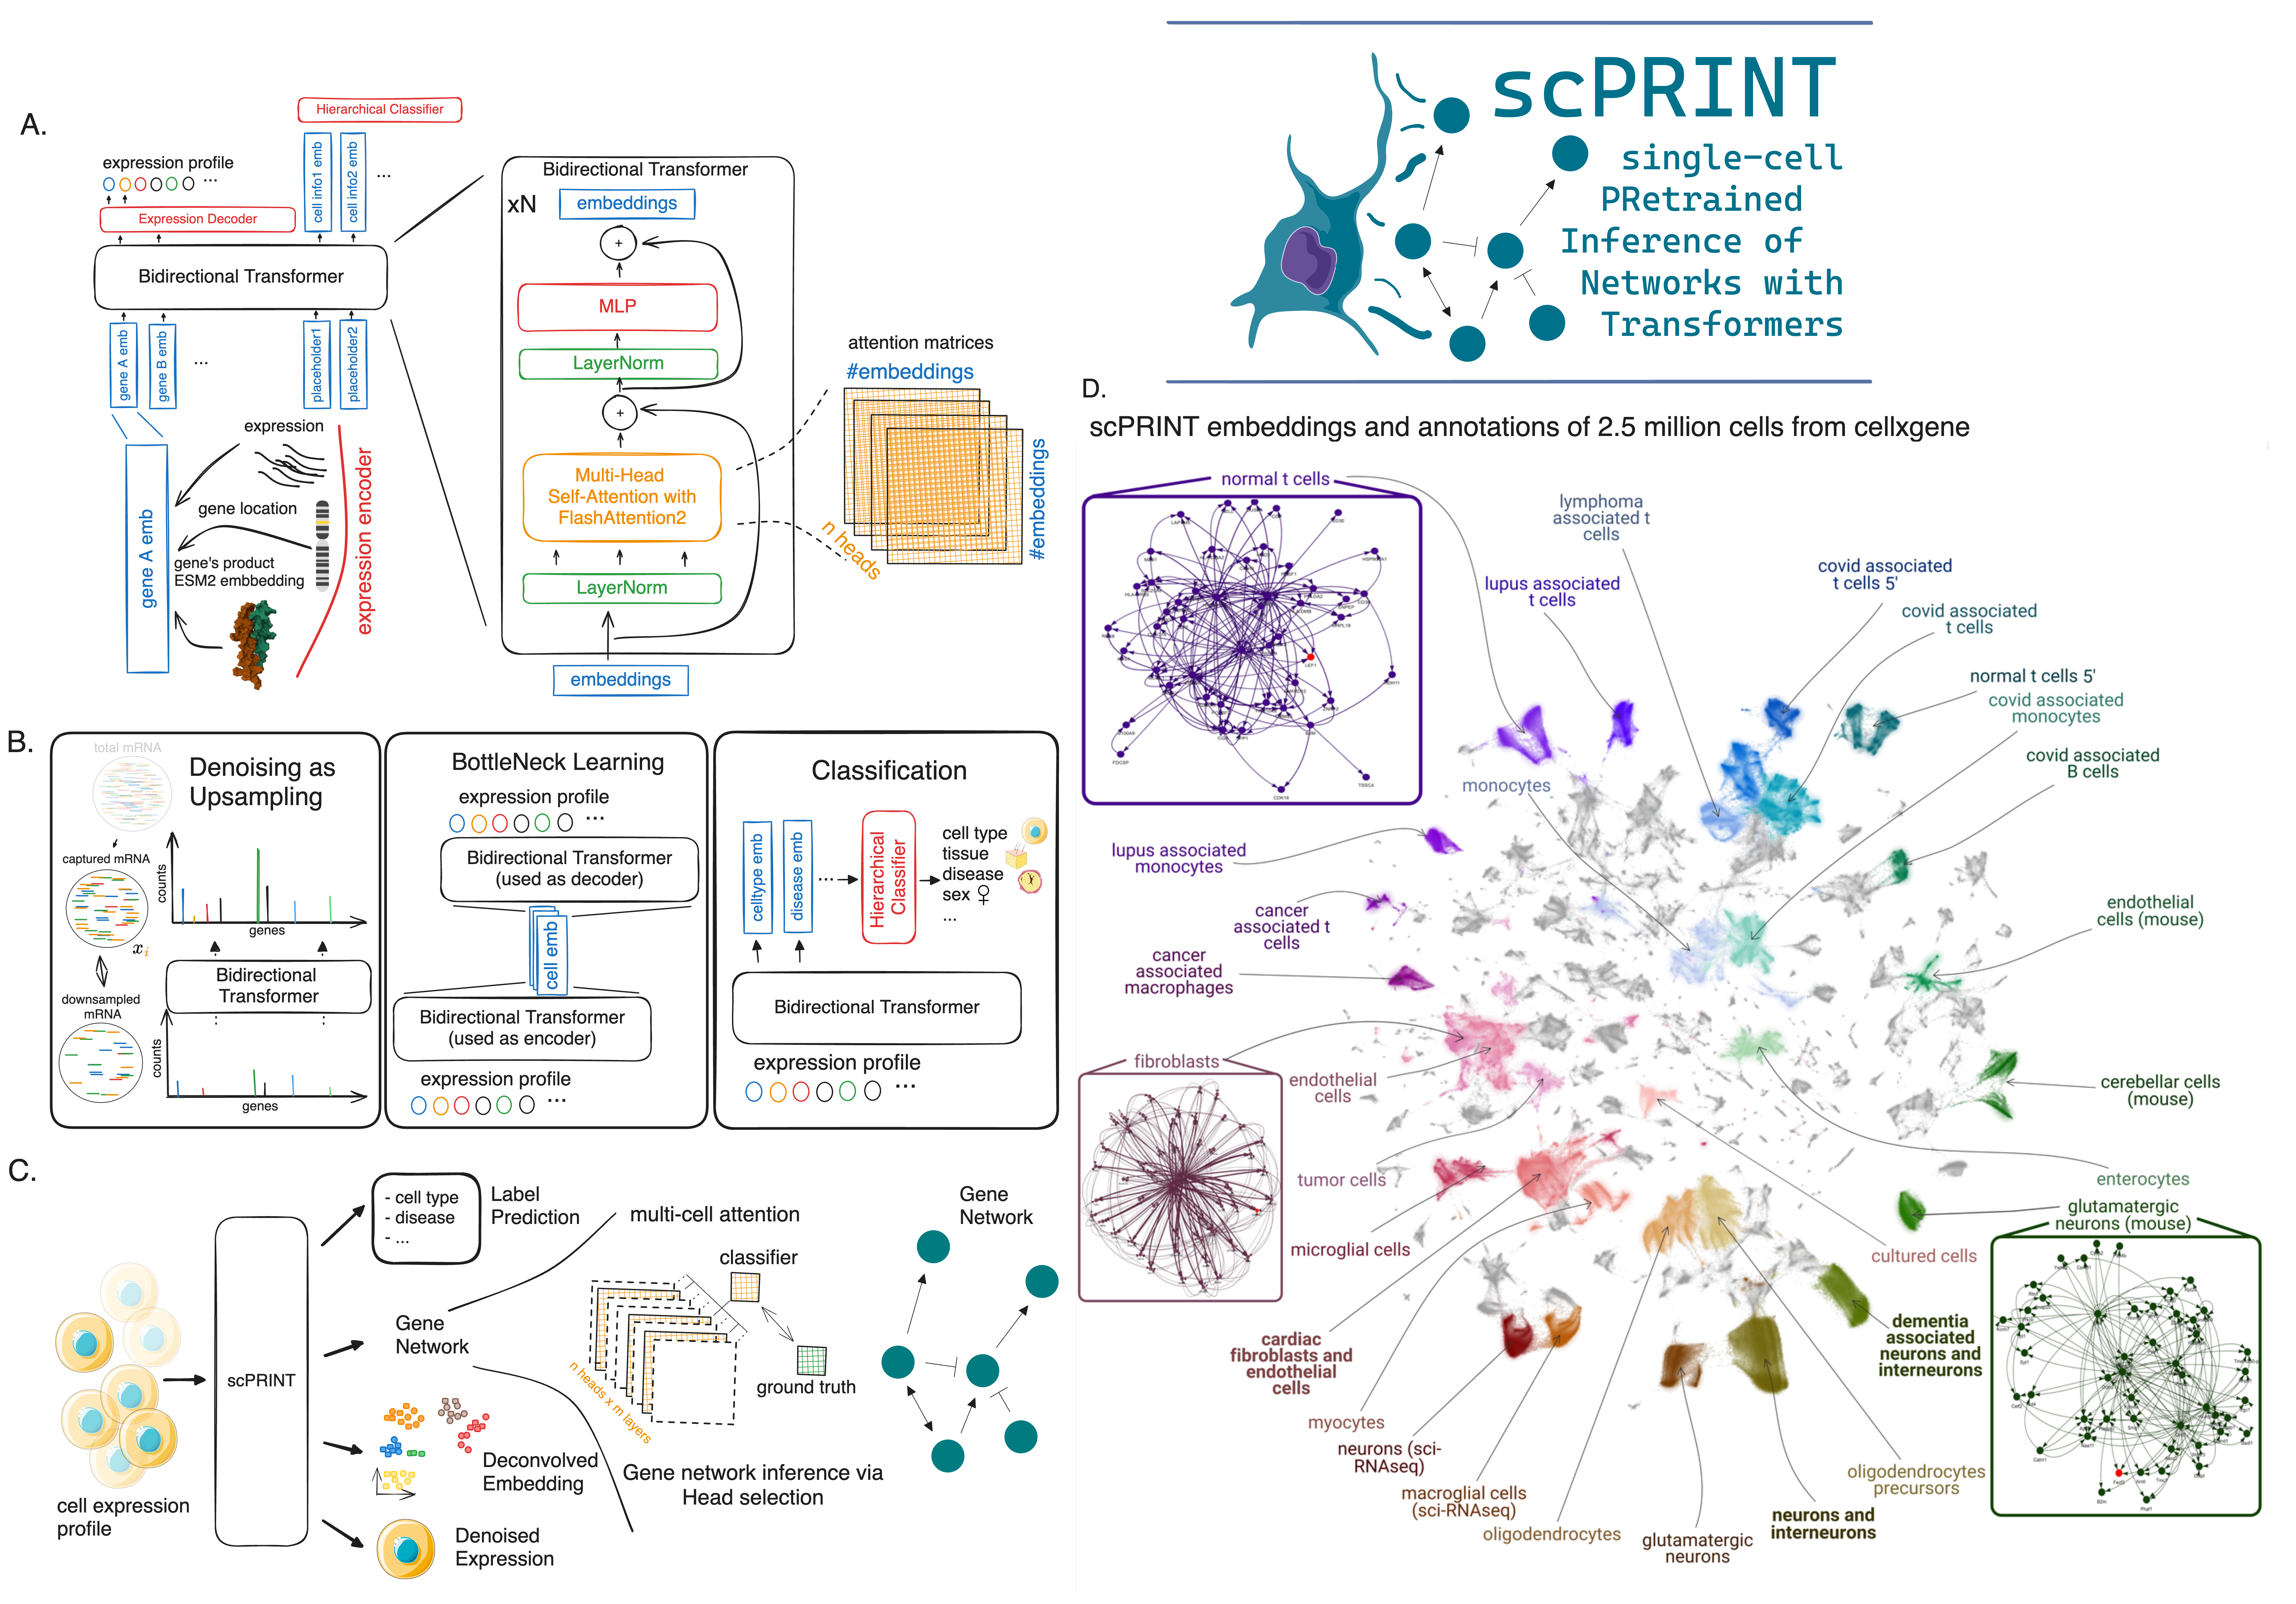
\includegraphics[width=0.9\textwidth]{figures/scprint/figure1}
    \caption[presentation of the scPRINT model and training]{(a) Schematic representation of \gls{scPRINT} with its bidirectional encoder, gene expression embedding encoding via gene location, matched protein \gls{ESM}2 embedding, and gene expression. (b) \gls{scPRINT} pre-training tasks: Denoising task whose goal is to recover the known transcriptomic profile from a purposefully downsampled expression profile. Bottleneck learning reconstructs the expression of requested genes using only their cell embedding. The same model is used for both The encoding and decoding steps. Hierarchical classification is achieved by applying a hierarchical classifier to each disentangled embedding. This pushes the first embedding to contain cell type info, the second embedding to contain disease info, and so on (see ~\ref{sec:methodsprint}. methods). (c) The different outputs in \gls{scPRINT}. \gls{scPRINT} generates label predictions of cell type, tissue, disease, sex, sequencer, ethnicity, and organism. \gls{scPRINT} generates multiple embeddings (which we call disentangled embedding), a general one, as well as a specific embedding for each class. \gls{scPRINT} also generates a reconstructed expression profile at any requested sequencing depth (i.e., total transcript count) (denoising). \gls{scPRINT} also generates a Gene Network by selecting and combining various attention heads into a gene x gene matrix. (d) Example of a \gls{scPRINT} output from a random subset of 2.5 million cells from the \gls{CxG} database. Embeddings and labels are generated by \gls{scPRINT}, together with the example cell type-specific gene networks. We show only subparts of the networks extracted from a central node, represented in red.}
    \label{fig:firstscprint}
\end{figure}

Thanks to the \gls{CxG} database requirement for complete annotations and our innovative hierarchical classifier, we have added label prediction as part of the pretraining of \gls{scPRINT}. While the assumption is that in other modalities, the scarcity and noisiness of such labels make it infeasible, we show that this approach is a net positive in our case (see ~\ref{sec:suppscprint}. Supplementary Table S3, ~\ref{sec:methodsprint}. Methods). Indeed, it helps us disentangle the various cell embeddings and performs zero-shot predictions on unseen datasets. These disentangled embeddings are opening a future possibility to perform counterfactual generation: mixing embeddings representing different facets of cell states, e.g., fibroblast + cancer + pancreas tissue + female, to generate novel unseen expression profiles.

\gls{scPRINT} converts the gene expression of a cell to an embedding by summing three representations or tokens: its id, expression, and genomic location (Figure ~\ref{fig:firstscprint}A, see ~\ref{sec:methodsprint}. Methods). \gls{scPRINT} encodes the gene IDs using protein embeddings. This gene representation is made using the \gls{ESM}2\citep{rivesBiologicalStructureFunction2021} amino-acid embedding of its most common protein product (see ~\ref{sec:suppscprint}. Supplementary Figure S1). First proposed in \gls{UCE}\citep{rosenUniversalCellEmbeddings2023}, the model learns to leverage representations that can potentially apply to unseen genes and species, using the structural and evolutionary conservation of the sequence encoded by \gls{ESM}2. While drastically reducing the number of weights used in the model compared to \gls{scGPT} and Geneformer (see ~\ref{sec:methodsprint}. Methods), this representation also contains some priors needed to infer protein-protein\citep{huImprovingProteinproteinInteraction2024} interactions (Figure ~\ref{fig:firstscprint}A). 

The gene's expression is tokenized via a \gls{MLP} using log-normalized counts. This \gls{MLP} lets the model learn a metric behind gene expression, whereas \gls{scGPT} and Geneformer apply a specific prior for the encoding of their gene expression (see ~\ref{sec:methodsprint}. Methods).

Finally, we help the model know that genes with similar locations tend to be regulated by identical \gls{DNA} regions, using the positional encoding of their location in the genome (see ~\ref{sec:methodsprint}. Methods).

These three embeddings are summed and then concatenated across all the genes expressed in a cell together with additional placeholder cell embeddings to form the transformer model's input.

\gls{scPRINT} is pretrained using 2,200 randomly selected expressed genes in a cell profile. If a cell doesn't have enough expressed genes, the list is padded with randomly selected unexpressed genes. A context of 2200 genes, while not genome-wide, captures all the expressed genes in more than 80\% of the cell profiles in the \gls{CxG} database. We also show that \gls{scPRINT} can make predictions on much larger sequences of genes at inference time without using attention approximation methods\citep{choromanskiRethinkingAttentionPerformers2022}.

Using unexpressed genes, combined with the denoising task, let \gls{scPRINT} discriminate the true zeros from dropouts in \gls{scRNA-seq}47. The expression decoder of \gls{scPRINT} further helps model this statistic of the data. It is a zero-inflated negative binomial graphical model inspired by previous literature in single-cell \gls{RNA-seq} modeling48. Here, the loss (also used for bottleneck learning) is thus the log-likelihood of the gene expression given the distribution parameters.

As shown in Figure ~\ref{fig:firstscprint}C, at inference time, \gls{scPRINT} can generate multiple outputs across any \gls{scRNA-seq}-like cellular profile of various mammalian species without fine-tuning. Figure ~\ref{fig:firstscprint}D shows \gls{scPRINT}'s prediction at the scale of an atlas of 2M randomly sampled cells from \gls{CxG}. From its pre-training, \gls{scPRINT} performs denoising, label prediction, and cell embedding without fine-tuning. However, a critical emergent output of \gls{scPRINT} is its cell-specific gene networks. Following a similar approach to \gls{ESM}2, we generate cell-level gene networks via the bidirectional transformer's input-wise weighted matrices, called attention matrices -or heads-. They represent general gene-gene connections and can be subsetted to \gls{TF}-gene connections (i.e., \gls{GRN}s). Remarkably, we made this approach scalable enough to compute attention heads-based gene networks for 1 to 10,000 cells, at the genome scale, with commodity hardware and in a few minutes. These networks both showcase the ability of \gls{scPRINT} to model cellular biology and help make it a more explainable tool for the community, showing the network assumptions made during inference. The attention heads are either all aggregated by averaging or can be selected to better reflect connections of interest (Figure ~\ref{fig:firstscprint}C). This is done using the average of the heads most correlated with literature or perturbation-based ground truth networks. Finally, while we do not assess \gls{scPRINT}'s ability to model inhibition due to the scarcity of such annotations, we leave open the possibility of using our head selection technique for such a task. 

Similarly to what has already been done in \gls{ESM}2 and the Large Language Model literature\citep{abnarQuantifyingAttentionFlow2020,clarkWhatDoesBERT2019a,bibalAttentionExplanationIntroduction2022}, we deeply investigate the meaning of attention matrices in the context of cellular biology, an aspect under-studied in the literature of foundation models applied to genomics. 

In the following sections, we benchmark \gls{scPRINT} on gene network inference against \gls{scGPT}, Deep\gls{SEM}\citep{shuModelingGeneRegulatory2021}, GENIE3\citep{huynh-thuInferringRegulatoryNetworks2010}, and Geneformer v2\citep{chenQuantizedMultitaskLearning2024}, the updated version of Geneformer. \gls{scGPT} and Geneformer v2 are highly cited and published transformer models for single-cell \gls{scRNA-seq}, mentioning the inference of gene interactions\citep{cuiScGPTBuildingFoundation2024}. Deep\gls{SEM} is an autoencoder model jointly learning its weights and a gene network matrix. GENIE3 generates networks via regression by finding the set of genes that best predict another gene's expression. It is one of the top-performing and most used methods for \gls{GRN} inference (see ~\ref{sec:methodsprint}. Methods). However, it suffers from very long run times and high memory requirements (see ~\ref{sec:suppscprint}. Supplementary Table S4).

\subsection{scPRINT recovers biological features in its gene networks}

We benchmark \gls{scPRINT} against the \gls{SOTA} based on whether their recovered networks contain meaningful biological knowledge. We consider two main benchmarking methodologies, one using a simulated expression profile from a well-established biological network. Because simulated data does represent real cell expression data (see ~\ref{sec:methodsprint}. Methods), our second and main approach focuses on biological features of a network inferred from real cell expression profiles. Indeed, we assume that a meaningful gene network should have some of its hub nodes being \gls{TF}s. \gls{TF}s should be more connected to their known target, on average. We should recover known gene-gene connections and expect enrichment of cell type-specific marker genes in the network.

We compare each gene network inference method's ability to recover a known network from 1000 simulated single-cell \gls{scRNA-seq} expression profiles generated by the Sergio \gls{ODE} model\citep{dibaeiniaSERGIOSingleCellExpression2020} from the ground truth network Regnetwork\citep{liuRegNetworkIntegratedDatabase2015} (see ~\ref{sec:methodsprint}. Methods). Only \gls{scPRINT} was able to recover meaningful connections (see ~\ref{sec:suppscprint}. Supplementary Table S5). One explanation is that through its training, \gls{scPRINT} has learned the common gene connections that also exist in the RegNetwork ground truth.

\begin{figure}[H]
    \begin{center}
        \includegraphics[width=0.8\linewidth] {figures/scprint/figure2}
    \end{center}
    \caption[Analysis of the gene networks generated by \gls{scPRINT}]{(a) We extract cell type-specific gene networks for each cell type in the dataset (n=26 cell types across 3 datasets). We perform Gene Set Enrichment Analysis (\gls{GSEA})\citep{subramanianGeneSetEnrichment2005a} on the network's nodes (n=4000 genes). We compute the ability of the edges to recover the Omnipath ground truth's connections. (b) Violin plot of the ten different \gls{AUPRC} and \gls{EPR} values obtained when comparing the inferred cell type-specific networks with the Omnipath network for \gls{scPRINT}: average of all attention heads, \gls{scPRINT} (genome): same \gls{scPRINT} version but computing a genome-wide gene network, \gls{scPRINT} (omnipath's heads): same \gls{scPRINT} version but with attention heads selected using a subset of omnipath, \gls{scGPT}, Deep\gls{SEM}, Geneformer v2, and GENIE3, when considering only \gls{TF}-gene connection or all gene-gene connections. (c) Violin plot of the average number of \gls{TF} with enrichment for their \gls{ENCODE} target in each cell-type-specific network. (d) Number of \gls{GN}s with a significant enrichment of \gls{TF}s and of their cell type's marker genes.}
    \label{fig:secondscprint}
\end{figure}

On gene network inference from real expression data, we noticed that depending on cell type and datasets, the different tools could vary greatly in the similarity of their \gls{GN}s to the Omnipath\citep{tureiOmniPathGuidelinesGateway2016} ground truth. Because of this, we focused our benchmark on three randomly selected test datasets of kidney, retina, and colon tissues comprising 26 cell types\citep{marshallHighresolutionSlideseqV2Spatial2022,wangSinglecellMultiomeHuman2022b,kongLandscapeImmuneDysregulation2023} (see ~\ref{sec:methodsprint}. Methods, per dataset results in \ref{sec:suppscprint}. Supplementary Figure S2). Of note is that we could not determine if these datasets were used during the training of \gls{scGPT} or Geneformer. 

We build one network per cell type, using the same 1024 cells and their 5000 most differentially expressed genes for all benchmarked methods. We evaluate the quality of the networks based on their overlap with Omnipath. We also compute the network enrichment for cell type markers, \gls{TF}s, and \gls{ENCODE} \gls{TF} targets using the prerank\citep{subramanianGeneSetEnrichment2005a} algorithm (Figure ~\ref{fig:secondscprint}A).

Although the \gls{scGPT} code mentions \gls{GRN} inference only using perturb-seq data, we reapply the same method without the perturbation-baseline comparison. This is to make it comparable with other benchmarked methods and because most of our datasets are not perturbation-based. Similar to what is presented in its paper, we use the mean of the attention matrices across cells and the four attention heads of the last layer of the human pre-trained model. We retain this method across our benchmarks for \gls{scGPT} (see ~\ref{sec:methodsprint}. Methods). We apply a similar strategy for Geneformer (see ~\ref{sec:methodsprint}. Methods).

For \gls{scPRINT}, we generate three network versions: one simply called \gls{scPRINT}, based on the average of all heads in the model. \gls{scPRINT} (omnipath's heads), based on the average of heads selected with our abovementioned head selection method inspired by \gls{ESM}2, and \gls{scPRINT} (genome), which is like the \gls{scPRINT} network but uses our method to generate genome-wide networks (see ~\ref{sec:methodsprint}. Methods) instead of using the 5000 most differentially expressed genes. Indeed, in transformer models, the choice of attention heads is important. Although transformers can learn the causal structure of their input, it has been shown that some attention heads, especially in larger networks, can become unused, containing predominantly random connections\citep{nichaniHowTransformersLearn2024}. Some work has been done at pruning these heads\citep{shimLayerwisePruningTransformer2021} or forcing a head selection mechanism during inference and training\citep{fedusSwitchTransformersScaling2022}. For \gls{scPRINT} (omnipath's heads), we select heads based on a linear classifier's prediction of the best set of heads to predict a subset of Omnipath (see ~\ref{sec:methodsprint}. Methods). Similarly to the \gls{scPRINT} network, these heads are then averaged to generate the \gls{scPRINT} (omnipath's heads) gene network. To perform this selection, we split the omnipath dataset into train/test and select heads, using 50\% of the ground truth and only the first cell type of each dataset. We then use the same combination of heads across all other cell types. This shows that our selection process builds consistent networks across cell types and parts of the ground truth. This innovative approach contrasts with previous ones like \gls{scGPT}'s and GENIE3 by using part of an available ground truth to select heads.

First, we look at how much information from Omnipath is contained in the inferred networks. Omnipath contains around 90,000 curated gene-gene connections, mainly from the literature. These connections are cell type agnostic, and most are \gls{TF} - gene. On this benchmark, we evaluate the networks based on \gls{AUPRC} and \gls{EPR}, two metrics often used in \gls{GRN} benchmarks\citep{pratapaBenchmarkingAlgorithmsGene2020} (see ~\ref{sec:methodsprint}. Methods), where we define our task as a binary classification of connections on all gene-gene pairs. Due to the row-wise normalization of networks generated by all methods, and because Omnipath has many sources with only a few targets (see ~\ref{sec:suppscprint}. Supplementary Figure ~\ref{fig:secondscprint}), we here use the transpose of our inferred networks when making comparisons with Omnipath (see ~\ref{sec:methodsprint}. Methods).
In Figure ~\ref{fig:secondscprint}B, we can see that \gls{scPRINT} (omnipath's heads) outperforms all methods on average across all cell types. While \gls{scPRINT} (omnipath's heads) uses some ground truth information to select its head, we see that \gls{scPRINT} still outperforms \gls{scGPT} and Geneformer v2 on the \gls{EPR} metric, showing that its top predicted edges more closely match the ground truth. 

\gls{AUPRC} results are very low overall because we do not expect most Omnipath connections to be present in the cell type's gene network, as many connections in Omnipath might only be true in some cellular contexts. Moreover, we do not expect most connections in our generated network to exist in Omnipath as it only contains a small fraction of all real gene-gene connections. Although overall \gls{AUPRC} values are small, we can see that both \gls{scGPT} and \gls{scPRINT} outperform the other methods in the number of connections recovered. Indeed, on average, \gls{scGPT} and \gls{scPRINT} respectively recover 42\% and 67\% more connections than GENIE3.

However, GENIE3 is often used by biasing the method to only predict \gls{TF}-gene connections (see ~\ref{sec:methodsprint}. Methods). This type of network, usually called a \gls{GRN}, is most often used, given the importance of \gls{TF}s in regulating gene expression. To compare the other methods to this \gls{GRN} version of GENIE3, we also use a \gls{GRN} version of their networks by subsetting them to \gls{TF}-gene connections only. In this context, all the methods significantly improve their predictions without altering their relative performances (Figure ~\ref{fig:secondscprint}B). This is unsurprising, considering that Omnipath is strongly biased towards \gls{TF}-gene interactions. 

Interestingly, we have seen that smaller \gls{scPRINT} models containing fewer heads perform better when taking the average of their heads. In contrast, head selection is often more advantageous in larger models with more heads (see ~\ref{sec:suppscprint}. Supplementary Table S6). As presented at the beginning of the results section, it might be that as models become larger and less regularized, some heads tend to become unused and contain mostly noise. As a consequence, a head selection is advantageous in larger models. 

We also expect biologically meaningful gene networks to have their central nodes enriched for \gls{TF}s. In addition, because these networks are cell type-specific, we expect their central nodes to be enriched for some marker genes of their associated cell types (see ~\ref{sec:methodsprint}. Methods). In this regard, both \gls{scGPT} and \gls{scPRINT} achieve very similar and strong network enrichment for \gls{TF}s compared to GENIE3, Deep\gls{SEM}, and Geneformer v2, whose networks are not enriched for \gls{TF}s (Figure ~\ref{fig:secondscprint}C).

Moreover, amongst the 178 cell types we have marker gene sets for in pangaloDB\citep{franzenPanglaoDBWebServer2019}, all methods find some enrichment, especially GENIE3 and \gls{scGPT} (see ~\ref{sec:methodsprint}. Methods). We notice that selecting heads based on Omnipath significantly improves \gls{scPRINT}'s network enrichment for cell-type markers. Of note, our goal is not to annotate cell types from the gene network but mainly to showcase the network's cell type specificity. 

Finally, we also examine how much the connections of each \gls{TF} are enriched for that \gls{TF}'s target. Here, \gls{scPRINT} overperforms all other methods (Figure ~\ref{fig:secondscprint}D). In the \gls{scPRINT} networks, 20\% of the Transcription Factors for which we have data on \gls{ENCODE} have connections significantly enriched for their \gls{ENCODE}-validated gene targets\citep{liberzonMolecularSignaturesDatabase2015}. Interestingly, only our large cell model achieved a great performance, and \gls{scGPT} did not display any enrichment across the 26 cell types assessed. While we acknowledge that \gls{ENCODE} is used in the Omnipath database, we cannot expect  Omnipath to represent the \gls{ENCODE} targets. Indeed, it combines and processes 57 additional data sources to build its consensus network.

\gls{scPRINT} (genome) has been added despite its performance not being comparable to other methods. Indeed, comparing its overlap with Omnipath is unfair as it includes many more genes and connections, many of which will have almost no data on this ground truth. While \gls{scPRINT} (genome) showcases our ability to generate genome-wide networks, it also shows strong performances in \gls{TF} enrichment and \gls{ENCODE} \gls{TF}-target enrichments. This highlights that even at such a large scale, networks generated by \gls{scPRINT} are enriched in biological knowledge gained solely from its pre-training tasks.

Overall, we have shown that \gls{scPRINT} generates, in one forward pass, cell type-specific gene networks that are biologically meaningful. We will now examine them using cell type-specific ground truths extracted from orthogonal experiments.

\subsection{scPRINT outperforms the state of the art on cell type-specific ground truths}

Although we have shown that our networks represent meaningful biology, the Omnipath ground truth is literature-based and not cell type-specific. Here, we use two different modalities, perturb-seq\citep{dixitPerturbseqDissectingMolecular2016}, and \gls{ChIP-seq}\citep{parkChIPSeqAdvantages2009}, as ground truths to compare predicted gene networks against.

In the MCalla et al.\citep{mccallaIdentifyingStrengthsWeaknesses2023} ground truth, \gls{ChIP-seq}uencing and perturb-seq are intersected to get at the small subset of possibly direct connections between \gls{TF}s and genes for both human and mouse embryonic stem cells (ESC) (Figure ~\ref{fig:third}A, see ~\ref{sec:methodsprint}. Methods). We have seen that these ground truth networks show a different pattern than literature-based networks (see ~\ref{sec:suppscprint}. Supplementary Figure S3). Some \gls{TF}s regulate only a few genes, whereas others are highly connected.

To generate our networks, we use as input one human and two mouse ESC \gls{scRNA-seq} datasets from MCalla et al. with the addition of another human dataset from Yan et al.\citep{yanSinglecellRNASeqProfiling2013} Networks are generated over the same 1024 cells, and the 5000 most variable genes for all methods. For \gls{scPRINT}, three networks have been generated: one averaging all the attention heads (\gls{scPRINT}), one averaging heads selected based on how well they predicted Omnipath ground truth data: \gls{scPRINT} (omnipath's heads), and one averaging heads selected from one of the MCalla ground truths: \gls{scPRINT} (Han et al.'s heads). For more details, see the results section 2: \gls{scPRINT} recovers biological features in its gene networks. Of note, due to the small amount of genes assessed in the ground truth, we do not add the genome-wide network version here. Moreover, only the \gls{TF} version of GENIE3 and the \gls{TF}-gene subsets of the other method's networks are used since the ground truth only contains \gls{TF}-gene connections.

Contrary to Omnipath, some elements in these biological networks are highly connected, whereas many others display no connections. This imbalance means that a method predicting only the highly connected \gls{TF}s will perform well on the MCalla et al. benchmark. As a consequence, we are not transposing the attention matrix as done in the previous section.

\begin{figure}[H]
    \centering
    \includegraphics[width=0.9\textwidth]{figures/scprint/figure3}
    \caption[scPRINT GN inference performance on cell-type specific ground truths]{(a) The ground truths are generated via orthogonal sequencing assays on the same cell type. \gls{ChIP-seq} and perturb-seq are intersected for the MCalla et al. dataset on human (hESCs) and mouse (mESCs) Embryonic Stem Cells, whereas perturb-seq on the K562 cell line is only used for the genome-wide perturb-seq ground truth. (b) Performance of \gls{scPRINT}, \gls{scPRINT} (omnipath's heads): same \gls{scPRINT} version but with attention heads selected using a subset of omnipath, \gls{scPRINT} (Han et al.'s heads): same \gls{scPRINT} version but with attention heads selected using a subset of the Han et al.'s ground truth dataset, compared to GENIE3, Deep\gls{SEM}, Geneformer v2, and \gls{scGPT} on the MCalla et al. ground truth using the \gls{AUPRC} and \gls{EPR} on two human and two mouse ESC datasets. (c) Same as (b) but on the genome-wide perturb-seq dataset with \gls{scPRINT} (Han et. al.'s heads) replaced with \gls{scPRINT} (gwps' heads): same \gls{scPRINT} version but with attention heads selected using a subset of the genome-wide perturb-seq ground truth. \gls{EPR} and \gls{AUPRC} are provided here in one barplot, left to right.}
    \label{fig:third}
\end{figure}

Based on both \gls{AUPRC} and \gls{EPR}, \gls{scPRINT} outperforms all other methods on this benchmark (Figure ~\ref{fig:third}B). This means, for example, that when training GENIE3 to only predict a gene's expression based on \gls{TF} expressions, it is not selecting the right \gls{TF}s amongst the set of a few dozen assessed in MCalla et al.

\gls{scGPT}, Geneformer v2—and, in a few cases, \gls{scPRINT}—can have values worse than random guessing. Thus, their predictions are often specific to some \gls{TF}s but not necessarily the right ones (Figure ~\ref{fig:third}B).

It also appeared that selecting heads based on Omnipath, although helping slightly in one instance, is not a net benefit for this dataset (see ~\ref{sec:suppscprint}. Supplementary Table S9). This makes sense since MCalla et al. itself does not overlap much with Omnipath (see ~\ref{sec:suppscprint}. Supplementary Table S7). However, selecting heads based on the ground truth itself, only using 50\% of the connections available, shows substantial improvement. These same heads also show reliable behavior when using them on the second dataset of the same species. 

This shows that \gls{scPRINT} can better decipher direct from indirect \gls{TF}-gene connections than \gls{scGPT}, Deep\gls{SEM}, Geneformer v2, and GENIE3, although more tests would likely be needed. 

However, the results also highlight that the high imbalance (i.e., \gls{TF}s being not connected or highly connected) combined with the dataset size (i.e., only a few dozen \gls{TF}s assessed) and the low number of cells make the results in MCalla et al. very variable. Some of this might be true biology or explained by \gls{ChIP-seq}, which can be very noisy depending on the quality of its antibodies\citep{kidderChIPSeqTechnicalConsiderations2011}.

To answer this issue, we selected another dataset: genome-wide perturb-seq (\gls{gwps})\citep{replogleMappingInformationrichGenotypephenotype2022}. Here, we measured the effect on transcription of knocking out all expressed genes in the K562 cell line. We transformed it into a network using a cutoff of 0.05 on the significance level of each gene's differential expression before and after the KO of each other gene. Although this does not tell us which connections are direct or indirect, we now have a much broader set of connections over thousands of genes and better statistics to assess our gene network inference methods.

GENIE3 performs best, directly followed by \gls{scPRINT}. Interestingly, Geneformer v2 shows poor performance (Figure ~\ref{fig:third}C). Perturbation experiments are known to correlate somewhat to expression correlation, and this might explain GENIE3's strong performance. However, when using our head selection mechanism, \gls{scPRINT} (gwps' heads) outperforms GENIE3. Again in this dataset, selecting heads based on Omnipath does not help; the small overlap between the \gls{gwps} network and the Omnipath ground truth network seems likely to be the culprit (see ~\ref{sec:suppscprint}. Supplementary Table S7). These overlaps show that the three ground truth networks are very different and that a different set of heads predicts each type of ground truth. We also assess the networks on the \gls{TF}-gene only subset of the \gls{gwps} ground truth. Here, we see a large drop in performances for most methods, except GENIE3 (see \ref{sec:suppscprint}. Supplementary Figure S4).

Finally, we have seen that on both MCalla and \gls{gwps}, \gls{scPRINT} also predicts networks that agree with the Omnipath ground truth and are again enriched for cell type markers and \gls{TF}s (see ~\ref{sec:suppscprint}. Supplementary Table S8, S9).

Since \gls{GN}s can be seen as approximations of a cell model, we expect that when a tool has good internal cell models, it should generate meaningful results on tasks such as denoising, cell type prediction, embedding and batch effect correction, perturbation prediction, trajectory inference, and more. We will now focus on three tasks orthogonal to \gls{GN} inference to compare the ability of \gls{scPRINT} to the \gls{SOTA}.

\subsection{scPRINT is competitive on tasks orthogonal to GN inference}
\label{scprintcompet}

\begin{figure}[H]
    \begin{center}
        \includegraphics[width=0.8\linewidth] {figures/scprint/figure4}
    \end{center}
    \caption[Benchmark of \gls{scPRINT} on orthogonal tasks to \gls{GN} inference]{(a) Performance for a denoising task compared to \gls{SOTA} methods MAGIC and knnsmooth2 on 3 datasets (ciliary body, colon, and retina tissues) from \gls{CxG}. Here, we generate a noisy profile by downsampling 70\% of the cell transcripts and computing the Spearman correlation increase of the correlation between the denoised and the true profile compared to the one between the noisy and the true profile. (b) Performance on cell-type label prediction compared to \gls{SOTA} methods as well as CellTypist. Showing accuracy, F1 and macro-F1 scores for the open-problems human pancreas dataset. (c) The performance of \gls{scPRINT} as well as \gls{scGPT} and Geneformer v2 on batch effect correction on the human pancreas and lung datasets from the openproblems challenge showing the scIB aggregated score. They are compared to \gls{SOTA} methods which results were extracted from the openproblems benchmark. Unintegrated means only PCA was applied. (d) The scIB avgBIO score on both datasets.}
    \label{fig:fourth}
\end{figure}

To test the quality of the cell model learned by \gls{scPRINT}, we now consider denoising, cell type prediction, and batch effect correction as a representative set of classic \gls{scRNA-seq} and cellular biology benchmarks.

Similarly to our pretraining task, we simulate lower transcript count profiles and then ask \gls{scPRINT} and two other \gls{SOTA} methods, MAGIC\citep{dijkRecoveringGeneInteractions2018} and KNNsmoothing2\citep{wagnerKnearestNeighborSmoothing2018}, to recreate the true expression profile. We use Spearman correlation to the original gene expression profile as our metric. In Figure ~\ref{fig:fourth}A, we show the increase in correlation after denoising the downsampled profile on 3 test set datasets, composed of ciliary body, colon, and retina tissues\citep{wangSinglecellMultiomeHuman2022b,vanzylCellAtlasHuman2022,burclaffProximaltoDistalSurveyHealthy2022}, randomly selected from \gls{CxG} (see ~\ref{sec:methodsprint}. Methods). 

ScPRINT is competitive with both \gls{SOTA} methods, while contrary to MAGIC and KNNSmoothing2, it operates independently over each cell in the test set (see ~\ref{sec:methodsprint}. Methods). We have also seen a 10\% variability in denoising ability across the different datasets used (see ~\ref{sec:suppscprint}. Supplementary Table S10). This was similar across all tools and possibly related to the number of genes expressed in each dataset.

However, these test cases mostly contain very similar cell states, whereas denoising is helpful in cases with rare cell types or transitory cell states that have low cell counts by default. We show that since \gls{scPRINT} does not aggregate profiles over neighboring cells, it outperforms MAGIC and KNNsmoothing2 in rare cell states subsets of the datasets (respectively: pericytes microfold cells of epithelium of small intestine and microglial cells) with around 10 to 200 cells (Figure ~\ref{fig:fourth}A, ~\ref{sec:suppscprint}. Supplementary Figure S5). Computing MAGIC and KNNsmoothing2 over only this rare cell population gives even lower performances for MAGIC and creates an error for KNNsmoothing2 (see ~\ref{sec:suppscprint}. Supplementary Table S10). These results suggest that a good cell model reliably using learned gene-gene interactions can help denoise an expression profile.

For cell type classification, we expect \gls{scPRINT} to be able to find sets of genes that can predict a cell type across multiple batches and under the high dropout rate of single-cell \gls{scRNA-seq}. To evaluate cell type classification, we use the multi-batch benchmark pancreas dataset of openproblems, its metrics, preprocessing, and hyperparameter choices (see ~\ref{sec:methodsprint}. Methods)\citep{lueckenBenchmarkingAtlaslevelData2022,OpenproblemsbioOpenproblemsv22024}.

\gls{scPRINT} is a zero-shot predictor of cell labels. Indeed, it does not need to train on the dataset itself to make its predictions, unlike other methods that often need to use more than 70\% of the test dataset for training. \gls{scPRINT} also makes predictions over more than 200 cell type labels, while other methods often only predict a few cell types. Conversely, the other classifier methods, like Logistic Regression or XGBoost, and previous foundation models are trained or fine-tuned on the test dataset, thus giving a strong advantage over \gls{scPRINT}. We, therefore, also compare \gls{scPRINT} to the marker-based classifier CellTypist\citep{condeCrosstissueImmuneCell2022} and its pancreas marker database (see ~\ref{sec:methodsprint}. Methods). A method that also does not use the labels of the test dataset.

\gls{scPRINT} reaches 62\% classification accuracy, largely outperforming CellTypist (Figure ~\ref{fig:fourth}B, ~\ref{sec:suppscprint}. Supplementary Figure S6). Interestingly, with the macro F1 score, which considers each cell type group equally regardless of its size, \gls{scPRINT} achieves similar results to the \gls{SOTA}\citep{OpenproblemsbioOpenproblemsv22024} methods: Logistic Regression and XGBoost. This is probably because \gls{scPRINT} is not influenced by the number of cells in each category.

In addition, we have noticed that \gls{scPRINT} is challenged by some specific pancreatic cell types in this dataset. Indeed, \gls{scPRINT} often switches the assignment of A, B, D, and E cells. Thus, when using the coarser “endocrine pancreatic cell” label to define these cell types, we see a big improvement in the accuracy and macro-F1 score of \gls{scPRINT}, even outperforming \gls{SOTA} methods.

Here, we have shown the accuracy of \gls{scPRINT} independently of cell neighborhood. However, like gene marker-based methods, \gls{scPRINT} can annotate cell types in novel datasets. In this context, its predictions could be smoothed and improved using majority voting over predefined cell clusters.

Finally, \gls{scPRINT} predictions are given as probability vector overall cell type labels. They can be used to display the top K labels and learn about the model's uncertainty.

Thanks to its disentangled embeddings, \gls{scPRINT} can generate cell representations that partially remove batch effects from cell profiles. On the human pancreas and lung datasets of open problems\citep{sikkemaIntegratedCellAtlas2023}, we see that, based on the \gls{scIB} metrics, \gls{scPRINT} shows convincing batch effects removal ability, while not on par with the \gls{SOTA} methods \gls{scGEN} and \gls{scVI} (Figure ~\ref{fig:fourth}C, ~\ref{sec:suppscprint}. Supplementary Figure S7). Concerning foundation models, \gls{scPRINT} and scFoundation show strong zero-shot performances compared to Geneformer v2 and \gls{scGPT}. Except for Geneformer v2, \gls{scGPT}, and scFoundation, we did not rerun previous algorithms for this benchmark and show their performances from the openproblems portal (open-problems-v2.3.6, march 2024). However, we also ran the Geneformer v2 and \gls{scGPT} foundation models on the openproblems benchmark and showed that without fine tuning on this specific dataset, they are not able to meaningfully correct for batch effect (see ~\ref{sec:methodsprint}. Methods).

Moreover, \gls{scPRINT} is one of the few methods that do not train on the test dataset and do not use already annotated batch labels. When only looking at methods that do not use batch labels as prior information, e.g., SAUCIE\citep{amodioExploringSinglecellData2019}, LIGER\citep{liuJointlyDefiningCell2020}, \gls{scPRINT} is the top performer. We have also noticed that the \gls{scPRINT} cell embeddings preserve biological information competitively to \gls{SOTA} methods (Figure ~\ref{fig:fourth}D, ~\ref{sec:suppscprint}. Supplementary Figure S8). This also exemplifies that a reliable cell model can perform well at disentangling the different facets of a cell expression profile and its underlying batch effect.

Overall, we have seen that \gls{scPRINT} can achieve zero-shot performances on par with many famous single-cell \gls{scRNA-seq} tools on multiple important tasks of single-cell biology, showing that our architecture and foundational pre-training tasks are a powerful new foundation for large cell models.

\subsection{scPRINT highlights the role of ion exchange and fibrosis in the ECM of Benign Prostatic Hyperplasia}

To showcase the ability of \gls{scPRINT}, we focus on premalignant neoplasms from an atlas of two studies of human prostate tissues\citep{josephSingleCellAnalysis2021}. The data contains both normals and pre-cancerous lesions, also called \gls{BPH}, across sequencers and age groups. Starting from post-alignment raw counts, \gls{scPRINT} generates a consistent and batch-corrected embedding of the datasets (Figure ~\ref{fig:fifth}A, ~\ref{sec:suppscprint}. Supplementary Figure S9). \gls{scPRINT} also annotates the cell type, sequencer, sex, ethnicity, and disease type of each cell with an accuracy of 0.71, 0.99, 0.99, 0.95, and 0.85, respectively.

\begin{figure}[H]
    \begin{center}
        \includegraphics[width=0.8\linewidth] {figures/scprint/figure5}
    \end{center}
    \caption[scPRINT-based bioinformatics analysis of early prostate cancer]{(a) Single-cell \gls{scRNA-seq} atlas of \gls{BPH} and normal prostate tissues of 83,000 cells given to \gls{scPRINT}. \gls{scPRINT} generates a set of embeddings and label predictions for each cell. To clean our predictions, we drop cell types with less than 400 cells and diseases with less than 1000 cells, replacing them with the “other” label (see ~\ref{sec:suppscprint}. Supplementary Figure S8). (b) Zooming in on one cluster, we see annotations of a switched memory B-cell cluster, some labeled "benign hyperplasia" and others "normal". Differential expression analysis on the two groups of B-cells showing enrichment of B-cell \& cancer markers when assessing its top 10 genes. We performed upsampling of the transcript count before performing a new differential expression analysis where we now see new genes amongst the top 10 differentially expressed ones some of them also associated with cancer and immune tissues.}
    \label{fig:fifth}
\end{figure}

We then focus on a switched memory B-cell cluster composed of a group of cells labeled as benign prostatic hyperplasia and another as normal (Figure ~\ref{fig:fifth}A). B-cells are known to be dominant in prostate cancer and are often switched memory B-cells\citep{saudiImmuneActivatedCellsAre2023}. First, we show that they differentially express many known B-cell markers (see ~\ref{sec:suppscprint}. Supplementary Figure S10). In addition, when comparing the \gls{BPH} to the normals B-cells, we recover that the top 10 \gls{BPH} B-cells differentially expressed genes contain many known cancer markers, B cell markers, and a specific B-cell associated prostate cancer markers: BAG5\citep{Bcl2AssociatedAthanogene} (highlighted in Figure ~\ref{fig:fifth}B, Table S11). Moreover, many other genes have evidence in other cancers, like CLIC4, known to be involved in the maintenance of the \gls{TME} in breast cancer\citep{HostCLIC4Expression}.

However, the number of healthy cells, especially normal memory B-cells, in this dataset is small: only 26. By performing denoising, we can recover genes that might have been missed during differential expression analysis of such a low cell count. Increasing the counts of all the genes by a factor of ten and re-doing differential expression analysis highlights some new genes whose differential expression scores are even higher than those previously cited. 

Interestingly, amongst them, TSEN54, EHMT2, and IL10RB are known to impact the function of B-cells in malignancies (see ~\ref{sec:suppscprint}. Supplementary Table S11). Other genes have evidence in immunity and cancer, like TAP1, which is known to be highly expressed in immune organs and is an immunomodulation gene known to play many roles in various cancers\citep{zhuTAP1PotentialImmunerelated2023}, while some genes have, of yet unknown significance, like LIP, whose paralog LIPA is a known cancer target\citep{TargetingLIPAIndependent} (Figure ~\ref{fig:fifth}B). 

This demonstrates how \gls{scPRINT} can embed, align, and annotate diverse datasets in a meaningful way so that one can then analyze specific and rare cell clusters to recover both known and new biology.

Finally, for the second part of the analysis, we move to another cell type of interest: fibroblasts. Fibroblasts are known to be involved in cancer\citep{CancerassociatedFibroblastsBasic}, also called cancer-associated fibroblasts (\gls{CAF}s), of which many subtypes exist, with different roles in tumor progression and invasion\citep{FibroblastHeterogeneityProstate}. In our dataset, we can see a large cluster of cells labeled as “fibroblast of connective tissue of glandular part of prostate”, of which 500 are coming from normal tissues, and 600 are coming from hyperplasia and are possible precursors of \gls{CAF}s (Figure ~\ref{fig:sixth}A). Interestingly, 40\% of the cells annotated as \gls{BPH}-associated fibroblasts are coming from healthy tissue, according to the authors of the dataset. However, it is known that more than 50\% of adult males over the age of 50 will have \gls{BPH}\citep{EpidemiologyClinicalBenign}. Thus, one possibility is that some of the fibroblasts of these healthy tissues already present patterns of gene activation similar to those of pre-cancerous ones. 

We generate a gene network of the \gls{BPH} and normal fibroblasts using the 4000 most variable genes and taking the average over all heads in the network (Figure ~\ref{fig:sixth}A). Looking at the top 15 hubs, using degree centrality, we can see S100A6 as the top element in normal fibroblasts. This gene is known to be a fibroblast and epithelial cell marker that regulates, among other things, cell cycle and differentiation\citep{kuznickiCalcyclinMarkerHuman1992,S100A6MolecularFunction}. We also see MIF, IGFBP7, and other genes involved in immune signaling and growth\citep{WikiPathways2024Next,ROLEBIOMARKERMACROPHAGE,IGFBP7PromotesEndothelial}.

\begin{figure}[H]
    \begin{center}
        \includegraphics[width=0.8\linewidth] {figures/scprint/figure6}
    \end{center}
    \caption[scPRINT-based bioinformatics analysis of early prostate cancer predicts disease cell-type specific gene networks]{Continuing on the single-cell \gls{scRNA-seq} atlas of \gls{BPH} and normal prostate tissues of 83,000 cells given to \gls{scPRINT} (a) Zooming in on another cluster from \gls{scPRINT}'s cell embeddings and annotations, we see a group labeled as "fibroblast of connective tissue of glandular part of prostate", some labeled as "benign prostatic hyperplasia", and others "normal". We generate gene networks from each and highlight a sub-network of the PAGE4 differential hub gene in \gls{BPH}, showing different connection strengths and patterns between normal and \gls{BPH}-associated fibroblasts. (b) Left to right: gene-set enrichment analysis, using Enrichr, of the gene community 4 found by the Louvain algorithm in the \gls{BPH}-associated fibroblast gene network, same but on the normal fibroblast gene network. It shows the top 10 most strongly enriched gene sets from GO\_MF\_2023 according to q-value (i.e. adjusted p-value).}
    \label{fig:sixth}
\end{figure}

However, some of these genes are not in common with the \gls{BPH} fibroblasts ones. Over the set of 2881 common nodes between the two networks, the genes HSPA1A, MT2A, SPOCK3, ATP6V0C, DEFA1, EIF4A1, and CD99 are considered differential hubs (i.e., more central) in the \gls{BPH} fibroblasts compared to normal ones (see Figure ~\ref{fig:sixth}A, Table S12). 

Another definition of centrality, eigenvector centrality, recovers 55\% of the genes already identified as hubs, plus some new ones. As an example, Prostate Associated Gene 4 (PAGE4), which is part of the GAGE family of genes, is expressed in a variety of tumors and reproductive tissues, especially \gls{BPH}, where it is related to oxidative stress response and fixation (i.e., anti-invasion)\citep{liProstateAssociatedGene42022,josephSingleCellAnalysis2021,lvPAGE4PromotesProstate2019}. Interestingly, although the networks share 75\% of their genes, they only share 50\% of their edges when considering the top 20 edges per gene. It shows that over the same set of genes, \gls{scPRINT} discovers distinct gene networks across biological contexts. Taking as an example the differential hub PAGE4 (Figure ~\ref{fig:sixth}A), we see that it is connected to many of the top 15 hub nodes in the \gls{BPH} network, such as MT2A, HSPA1A, SPOCK3, and CD99. This shows a master node sub-network linking metal and ion exchange, oxidative stress response, and inflammation\citep{diasDownregulationMetallothionein2A2022,luoMechanismPrognosticMarker2023,defreitasCirculating70KDa2022,CD99CrossroadsPhysiology}. Some genes are also part of the IL24 signaling inflammatory pathway (EIF4A1;COL6A2;HLA-C;HSPE1), and the secretory senescence phenotype (H2AZ1;UBE2S;UBE2C;IGFBP7)\citep{milacicReactomePathwayKnowledgebase2024}, hallmarks of fibrosis and malignancies\citep{mausIronAccumulationDrives2023,qianEstablishmentCancerassociatedFibroblastsrelated2023}. The PAGE4 network in normal fibroblasts, while having some elements in common, like metal transport, is much less connected (seen by the strength of the edges in Figure ~\ref{fig:sixth}A). It also contains a different set of genes, which are less related to senescence, inflammation, and ion exchange (see ~\ref{sec:suppscprint}. Supplementary Figure S11).

Furthermore, we can use these networks, defined over only a few cells, to perform community detection. Taking community 4, containing 92 genes and defined with the Louvain algorithm on the \gls{BPH}-associated fibroblasts \gls{GN}, we see two hub nodes: SPOCK3 and HERC3 (Figure ~\ref{fig:sixth}B). Interestingly, not much is known about those genes except that HERC3 has been linked to inflammation and the \gls{ECM} via metallopeptidase and the NCOA1 gene\citep{liAccumulationNCOA1Dependent2023}. SPOCK3, moreover, is known to be related to prostate malignancies and collagen in the \gls{ECM}\citep{luoMechanismPrognosticMarker2023}. Gene set enrichment tells us that the genes in this subnetwork are primarily related to calcium, sodium, iron, and metal transport, validating the evidence around HERC3 and SPOCK3 (Figure ~\ref{fig:sixth}B). In normal fibroblast, however, taking the community most associated with metal transport  (community 4, see details in ~\ref{sec:suppscprint}. Supplementary Figure S12 and Methods) shows RNASEK, SELENOM, and an unknown ubiquitin ligase, paralog of ITCH. While RNASEK is related to RNA degradation, its expression has been linked to a lower risk of prostate cancer\citep{kladi-skandaliExpressionalProfilingClinical2018}.  SELENOM is of unknown function, but some SEL proteins have been related to cell adhesion\citep{SelenoproteinDeficiencyAlters} . 

Through its networks, \gls{scPRINT} highlighted the role of ion exchange and fibrosis in the \gls{ECM} in \gls{BPH}. While some of the same genes would have been found from differential expression analysis, these results show us how gene networks can be used to describe the intersection of genes and their molecular functions. Putting genes into the context of their connections, one can validate known functions or relate them to new ones. From such contextualization, a picture starts to emerge, whereby through specific genes, glandular fibroblasts in senescence enter a wound-healing state. This fibrosis is caused by the export of more metal and ions to generate \gls{ECM} and change its acidity levels. This might cause a loss in tissue flexibility and potentially create oxidative stress\citep{EffectPHExtracellular}. In our networks, these pathways seem connected to inflammation. Chronic inflammation and wound healing states are hallmarks of \gls{BPH} and a predisposition to future malignancies\citep{colottaCancerrelatedInflammationSeventh2009,hanahanHallmarksCancerNext2011}.

\section{Discussion}

We can simplify the complex macromolecular interactions governing a cell through what is often referred to as a gene network. However, creating such a network in a meaningful way remains a challenging task.

We have created and benchmarked \gls{scPRINT}, a novel single-cell \gls{scRNA-seq} foundational model trained on more than 50 million single-cell profiles across tissues, diseases, and species contexts. \gls{scPRINT} uses three foundational pre-training tasks, as well as new encoding and decoding mechanisms specifically designed for gene expression data. Although it has not been directly trained for it, \gls{scPRINT} generates gene networks. These networks can be used to better understand the model predictions and help make more informed decisions about the significance and role of a potential target. Finally, we present a mechanism to best select heads containing the known biology of these networks. This approach also helps users fine-tune the type of network they are interested in. Given the discrepancy amongst ground truth networks, we advise users to consider using all-head averaging and to only revert to head selection when some high-confidence interactions are available. Indeed, general collections like Omnipath did not improve performance in most of our tests.

We show that we outperform other foundation models on most of our benchmarks while using a similar model size. We believe that our inductive biases and training procedures helped \gls{scPRINT} achieve such a performance. Moreover, while GENIE3 is still a competitive tool, we outperformed it on many of our benchmarks, showing that pushing training to millions of cells and large parameter sizes will be an essential direction for further work on gene network inference.

In addition, contrary to any other method assessed, our large cell model can also achieve zero-shot performances on par with many famous single-cell \gls{scRNA-seq} tools on multiple important cell biology tasks. While some specialized tools might be better suited to some use cases, \gls{scPRINT}'s versatility and speed make it a worthwhile alternative in many instances. Indeed, users can directly use \gls{scPRINT} in their bioinformatics workflows with commodity hardware (1 CPU, 1 \gls{GPU} with 10GB of memory and 16GB of memory).

Finally, we put \gls{scPRINT} to the test on a challenging atlas of normal and senescent prostate tissues showing \gls{BPH}. We identify rare cell populations with early markers of \gls{TME} in B-cells. In fibroblasts, we study gene networks and recover known hubs such as PAGE4, thereby linking the senescence of fibroblasts to changes in the \gls{ECM} and downstream inflammation. We find key interconnected pathways of the oxidative stress response and extracellular matrix building via metal and ion exchange in the gene network of \gls{BPH}-associated fibroblasts. We also show that healthy and disease-related cells exhibit different network patterns, demonstrating that \gls{scPRINT} can help identify novel pathways and targets while considering them in their specific cellular and molecular contexts.

An assumption in natural language processing is that fewer inductive biases make for better models. Our work shows that adding good inductive biases and rethinking architectures will likely be important directions for \gls{AI} models in biology. 

A challenging aspect of \gls{GN} inference is that no perfect ground truths exist, and many \gls{GN} methods are, unfortunately, benchmarked on \gls{ODE}-generated mock-up expression data. In contrast, \gls{ChIP-seq}, perturb-seq, and literature-based ground truths remain scarce and ambiguous. With BenGRN and GRnnData, our suite of tools for benchmarking Gene Networks inferred from single-cell \gls{scRNA-seq}, we present an extensive set of real-world ground truths representative of the diversity of networks we can assess. However, improvement in performance and benchmarking will need to come from innovative experimental approaches that can produce causal, genome-wide, and cell-type-specific networks containing the many different types of connections and regulations that exist, from \gls{PPI}, \gls{RNA}-\gls{DNA}, \gls{RNA}-protein, to inhibition, activation, cooperation, and more.

We acknowledge that work remains to be done, from the transformer's ability to generate graphs to their explainability and the breadth of tasks they can undertake. Questions still remain regarding the pre-training tasks and how to integrate additional data modalities into foundational models.

Transcription is much more complex than what gene networks currently represent. In the future, we expect such large cell models to work in tandem with new sequencing techniques measuring information such as time, space, protein amounts, \gls{DNA} configuration, and non-coding \gls{RNA} species to solve the gap in our understanding and our ability to model cell biology.

%\includepdf[pages=-]{chapters/scprint.pdf}
\section{Methods}
\label{sec:methodsprint}

we propose scPRINT, a foundation model designed for gene network inference. ScPRINT brings novel inductive biases and pretraining strategies better suited to GN inference while answering issues in current models. scPrint outputs cell type-specific genome-wide gene networks but also generates predictions on many related tasks, such as cell annotations, batch effect correction, and denoising, without fine-tuning.

\subsection{Architecture}\label{architecture}

The model architecture is composed of:

\begin{itemize}
\item
  An encoder that takes the raw data and embeds it in a high-dimensional
  space used by the transformer.
\item
  A bidirectional multi-head transformer
\item
  A decoder to transform the expression embeddings into expression
  values
\item
  A decoder that transforms the cell embeddings into cell-specific label
  prediction over a range of classes.
\end{itemize}

\subsubsection{Expression encoder}\label{expression-encoder}

In scPRINT, each gene in a cell is converted to an embedding: It
corresponds to the sum of 3 different elements:

1. An embedding representing the gene itself (see Supplementary Table \href{table-s1-list-of-novelties-in-scprint-and-comparison-to-scgpt-and-scfoundation} for model embedding size). ESM2 embedding of each gene's most common protein product was used to represent that gene. While imperfect in some ways, this inductive bias allows the model to learn representations that potentially apply to even unseen genes from unseen species or integrate specific genetic mutations into its representation. First implemented in UCE, this provides the model information related to the gene product's structure, ontology, and similarity to other genes. This also speeds up the training greatly, particularly for small models. We show that this is a great gene representation, but that model performance can be increased by refining gene embeddings further during training. However, we elect not to do so to maintain the model's versatility in working on unseen genes.

We encode the genes' embeddings using ESM2. The mapping process happens the following way:

\begin{itemize}
\item
  A gene name is mapped to its canonical protein name using Ensembl.
\item
  We recover the protein sequence of the protein using Ensembl
\item
  We use the protein sequence to generate an embedding using ESM2 by averaging all the amino-acid output embeddings, as done in the ESM2 paper.
\end{itemize}

With the embedding function provided in our code, one can easily do this with any species in Ensembl.

scPRINT can effectively be retrained with any set of gene embeddings, which can be frozen during training or used only for initialization (tried, for example, in our ablation studies, Table S3).

2. An embedding of the gene location in the genome. This has also been proposed in UCE and helps the model understand that genes with similar locations tend to be regulated by similar regulatory regions, a relationship well-known in cellular biology.

We encode the genes' locations using positional encoding. Every gene less than 10,000 bp from the next is said to be in the same location; otherwise, we increment location by 1. We do this for all genes in the Ensembl database per species.

We then embed these locations by applying the Positional Encoding (PE) algorithm of Vaswani et al. .

3. An embedding of the gene expression in the cell. For this, we embed
the gene's expression using an MLP. While GeneFormer devised a ranking
strategy based on a gene expression compared to a baseline expression,
scGPT instead used binning of log normalized counts. On our end, we
haven't found that this approach was the simplest, nor was it performing
better than only using the log-transformed counts. We thus directly take
the log-transformed counts

\begin{equation}
\mathbf{e}_{\mathbf{i,j}} = MLP(log_{2}(x_{i,j} + 1)),\ x_{i,j} \in \mathbb{R},\ \mathbf{e}_{\mathbf{i,j}} \in \mathbb{R}^{d}
\label{eq:expression_embedding}
\end{equation}

where \(\exp r_{i,j}\ \)is the embedding of the expression, \(x_{i,j}\)
is the expression value of the gene j in the cell i, and the MLP is a
two-layer neural network, where each layer is composed of

\begin{equation}
Dropout(ReLU(LayerNorm(Linear(\mathbf{e}_{\mathbf{i,j}}))))
\label{eq:mlp_layer}
\end{equation}

where the Dropout rate is fixed at 0.1, and the dimensions are specified
as 1 → \emph{d} for the first layer of the MLP and \emph{d → d} for the
second layer, with d representing the model dimension.

Of Note: Geneformer used positional encoding to encode gene expression,
a function often used to encode the position of words in a text.
Similarly to gene name token, scGPT learned an embedding for different
ranges of expression values, binning them to remove sampling noise.

Both approaches apply a specific prior for the metric that defines
expression. Geneformer defines expression amount as ranking based on how
each gene is expressed in the cell compared to its average across all
cells. Unregarding the batch effect issues, this is an assumption that
expression values are not meaningful and only the ranking of the
relative abundance is meaningful information. Meanwhile, scGPT has the
bias that an expression of 1, 2, or 3 are the same and that an
expression 1, and 5 are different by some amount learned by the model.

By using an MLP with two layers, we effectively let the model learn the
metric of transcription expression. Moreover, again, we decrease the
number of parameters used compared to scGPT while being able to make
predictions on count values unseen during training, such as those of
bulk or pseudo-bulk RNAseq.

Finally, when encoding a cell expression profile, only a subset of 2200
genes is used during pretraining. If less than 2200 genes are expressed,
we randomly choose 2200 expressed genes and pad them with randomly
sampled unexpressed genes (meaning with an expression value of 0). This
approach allows the model to see different patches of the same cell
profile during training. We chose 2200 genes as 2/3rds of the cells in
cellxgene had less than this number of genes expressed, striking a
balance between computation and gene usage.

We decided to add unexpressed genes because, combined with our denoising
methodology, this lets the model figure out that some genes are true 0s
during training. In contrast, others are only caused by dropout and a
function of the transcript counts. This causes scPRINT to model dropout
as a function of read depth (i.e., total transcript count).

Moreover, this completes the minibatch by token matrix without padding
and fully utilizes the GPU during the attention computation.

Of note, some models have been able to reach context lengths of 20,000
genes using the performer architecture. Performer is an often-cited
method and part of the literature on attention approximation. However,
most state-of-the-art transformer models do not use attention
approximation as they are known to lead to worse
performance.

Moreover, in cellxgene, more than 80\% of the cells have less than 2200
genes being measured. This means that most of the memory and compute
power is likely lost on tokens that are almost always zeros due to
dropout.

The full set of embeddings of cell i sent to the transformer is the
matrix \(X_{i}\) where

\begin{equation}
X_{i} = [\mathbf{g}_{\mathbf{0}} + \mathbf{e}_{\mathbf{i,0}} + \mathbf{l}_{\mathbf{0}}, \mathbf{g}_{\mathbf{1}} + \mathbf{e}_{\mathbf{i,1}} + \mathbf{l}_{\mathbf{1}}, ..., \mathbf{e}_{\mathbf{i,t}}, \mathbf{p}_{\mathbf{default}}, \mathbf{p}_{\mathbf{celltype}}, \mathbf{p}_{\mathbf{disease}}, ...]
\label{eq:cell_embeddings}
\end{equation}

where \(\mathbf{g}_{\mathbf{j}}\) is the gene j encoding,
\(\mathbf{e}_{\mathbf{i,j}}\) is the encoding of the expression of gene
j in cell i, \(\mathbf{l}_{\mathbf{j}}\) is the gene j location
encoding, and \(\mathbf{p}_{\mathbf{A}}\) is a learnt embedding for the
class A.

The total count information is stored separately and encoded similarly
to the expression,

\begin{equation}
\mathbf{e}_{\mathbf{t,i}} = MLP(log_{2}(1 + t_{i})), \text{ where } t_{i} = \sum_{j}x_{i,j}
\label{eq:total_count}
\end{equation}

with \(x_{i,j}\) the expression value of gene j in cell i, and the MLP
is a two-layer neural network similar to the previous one.

The full cell total count (\(t\)) lets scPRINT model its denoising based
on this required total count parameter.

The placeholder tokens (total count, default cell embedding, cell type,
disease, sex, ethnicity, assay, organism) are learned embeddings that
stay the same across all inputs. They only act as placeholders for the
model to fill in during the forward process. At the transformer's
output, they will have been modified to contain the embeddings
requested. At least two are used, one containing the default cell
embedding and another the profile's total depth. More tokens can be
used, one for each predicted cell label.

\subsubsection{Model}\label{model}

The model is a bidirectional autoencoder similar to
BERT with \emph{n} layers, \emph{h} attention heads,
and a dimension of \emph{d}. It uses the
flashattention2 methodology implemented in Triton to
compute its attention matrix. It uses the pre-normalization
technique, with a sped-up layer norm implemented in
Triton's tutorial. It uses a stochastic depth with
increasing dropout probability.

It has a 2-layer MLP with a 4x width increase in its hidden layer and a
GELU activation function.

\subsubsection{Expression decoder}\label{expression-decoder}

scPRINT uses a novel expression decoder for foundation models, which
outputs the parameters of a zero-inflated negative binomial
(\emph{ZiNB}) function for each gene \emph{i} in cell \emph{j}. The
\emph{ZiNB} distribution is defined as

\begin{equation}
X \sim ZiNB(\mu, \theta, \pi)
\label{eq:zinb_dist}
\end{equation}

where the parameters \(\mu,\ \theta,\ \pi\) are obtained from a
multi-layer perceptron (MLP) applied to the expression embeddings
outputted by the transformer model at its last layer (e), which are the:

\begin{equation}
\mu, \theta, \pi = MLP(\mathbf{e})
\label{eq:zinb_params}
\end{equation}

The MLP is a two-layer neural network with dimensions {[}\emph{d, d},
3{]}

Based on the work of Jiang et al., zero inflation is
the best distribution when considering a broad range of transcriptomic
measurements, where some have enough dropouts, and a zero inflation term
is needed to model it. In our case, and similarly to
scVI, we define our \emph{ZiNB} as

\begin{equation}
ZiNB(x | \mu, \theta, \pi) = \pi\delta_{0}(x) + (1 - \pi)NB(x | \mu, \theta)
\label{eq:zinb_def}
\end{equation}

where \(\delta_{0}(x)\) is a point mass at zero, and
\(NB(x\ |\ \mu,\theta)\) is the negative binomial distribution with mean
\(\mu\) and dispersion \(\theta\).

With these parameters, the negative binomial distribution is represented
in the following way

\begin{equation}
NB(x | \mu, \theta) = \frac{\Gamma(x + \theta)}{x!\Gamma(\theta)}\left(\frac{\mu}{\mu + \theta}\right)^{x}\left(\frac{\theta}{\mu + \theta}\right)^{\theta}
\label{eq:nb_dist}
\end{equation}

where \(\mu\) is the mean and \(\theta\) the overdispersion parameter,
representing the inverse of the dispersion. From Hibe et
al., we know that this is a parameter change from
the most used probability mass function (PMF) given by

\begin{equation}
P(X = x) = \binom{x + r - 1}{x}(1 - p)^{r}p^{x}
\label{eq:pmf}
\end{equation}

where r is the number of successes, \emph{p} is the probability of
success, and \emph{k} is the number of failures.

One can interpret such a negative binomial distribution as a Poisson
distribution with an additional overdispersion term that makes the
variance not tied to the mean. In scPRINT, we use the zero-inflated
Poisson for count downsampling as we can't easily infer the gene
overdispersion parameter from each cell profile. By removing this
zero-inflated Poisson from the gene expression profile, we keep the
potential overdispersion in the profile (see the
\hyperref[negative-binomial-to-poisson-relationship]{Negative Binomial
to Poisson relationship} section in Methods).

Compared to scVI, where the overdispersion parameter \(\theta\) is
learned for each gene, we make scPRINT output it together with
\(\mu,\ \pi\) (see Supplementary Figure \ref{fig-s13-graphical-model})

Effectively, the model learns that the dispersion might change depending
on the gene, the sequencer, the cell type, and the sequencing depth.

\subsubsection{Class decoder}\label{class-decoder}

scPRINT also outputs a variety of class embeddings, such as default cell
embedding, cell type embedding, disease embedding, etc., by filling the
different placeholder tokens given as input (see the
\hyperref[expression-encoder]{Expression encoder} section in the
Methods).

Effectively, for each class, we have the model learn to produce a new
disentangled embedding (e.g., cell type, disease, tissue, age). This
means the model uses an MLP to transform each token where A is a class.
For each, we jointly train a classifier:

\begin{equation}
\widehat{\mathbf{c}_{\mathbf{A}}} = \sigma(MLP_{A}(\widehat{\mathbf{e}_{A}}))
\label{eq:classifier}
\end{equation}

where:

\begin{itemize}
\item
  \(\widehat{\mathbf{c}_{A}}\ \)represents the logits for a class A of a
  dimension \(d_{A}\) whose size corresponds to the number of labels.
\item
  \(\sigma\) denotes the Sigmoid activation function.
\item
  \(MLP_{A}\) stands for the Multi-Layer Perceptron trained to predict
  the logits of the class \emph{A.}
\item
  \({\widehat{\mathbf{e}}}_{A}\) is the output embedding for the class A
  of dimension \emph{d}.
\end{itemize}

However, some classes, like cell type, have up to 800 labels.
Fortunately, cellxgene classes follow an ontology, a robust structure
that defines relationships among the labels. We reduce the size of the
output labels by training the model only on the leaf labels in the
ontology hierarchy (i.e., the most precise available). For cell types,
this represents around 400 different labels (see Supplementary Table \ref{table-s13-number-of-elements-predicted-per-class}).

Thus, when a label is not very specific for a cell type (e.g., neuron),
the model will predict the best leaf label (e.g., dopaminergic neuron).
This way, we can generate meaningful training signals from even very
coarse labels (see \hyperref[the-classification-task]{The classification
task} section in methods for more information and definition of the
loss). We only apply this hierarchical classifier to the cell type,
disease, and assay labels.

In the following section, we show how we train such classifiers. During
the classifiers' training, we sum up their loss without
applying any scaling between the different classes.

\subsection{Ablation study}\label{ablation-study}

We perform an ablation study of multiple of our additions in scPRINT for
its medium size version. Removing positional encoding, replacing
log-normalization with a total-normalization, replacing denoising with
masking, using the cell-gene product method of scGPT vs our own
encoder-decoder approach to learn a cell embedding, using 2 vs 4 heads
per attention blocks, not using weighted random sampling, not freezing
the gene ID embeddings, and using mean-squared-error instead of the ZINB
loss. For each, we re-train scPRINT entirely on the same dataset and
validate its test performance with our automated benchmark platform. We
provide the results in Table S3.

\subsection{Pretraining}\label{pretraining}

The three tasks of the multi-task pretraining are the denoising task,
the classification task, and the bottleneck learning task. While the
denoising loss enhances the model's ability to find
meaningful gene-gene connections, the other two try to make the model
and its underlying networks more robust and cell-type-specific. All
three losses are summed without rescaling.

\subsubsection{Optimization method}\label{optimization-method}

The optimization is done with fused ADAMW, with a weight decay of 0.01.
We noticed a total inability to learn when using base ADAM, which has a
similar weight decay. This can be explained by a known inequivalence
issue in ADAM.

We use the stochastic weight averaging method
during training with a learning rate of 0.03.

During pre-training, the hyperparameters are set to dropout of 0.1, a
learning rate (LR) of 1e-4, the precision is set to 16-mixed with
residuals in fp32. We clip gradients to 100 and train in many sub-epochs
of 7000 training batches and 2000 validation batches with a warmup
duration of 500 steps.

Across epochs, we use a linear LR decrease of 0.6 with a patience of 1
and stop training after three consecutive increases in validation loss
(patience: 3). In the final layer of the class decoders, we initialize
values to a normal distribution around 1 for weights, 0 for biases, and
-0.12 for biases.

Our batch size is 64, and we use a pre-norm strategy for the transformer
with a linearly increasing stochastic depth dropout rate of 0.02 per
layer. We use a noise parameter of 60\%. We split the cells in the
datasets into 98\% train and 2\% validation and reserve at minimum 2\%
of separated datasets for testing.

Finally, we use weighted random sampling on our training data based on
the different class values we have to predict. We use a factor of 50,
meaning the rarest elements will, on average, be sampled only 50 times
less than the most common ones. The sampling factor used for each group
is then \(\frac{50}{count + 50}\), instead of \(\frac{1}{count}\) where
count is the number of cells in each group.

\subsubsection{The classification task}\label{the-classification-task}

We perform label prediction during pretraining for different classes,
currently: cell type, disease, sequencer, ethnicity, sex, and organism.
Due to issues in the ontologies, we have omitted tissue type and age
classes.

Due to the hierarchical structure of the prediction, we also created a
hierarchical loss. Here, we compute the loss regularly when the label is
a leaf label. Otherwise, we replace all associated leaf labels to the
given label by the log-sum-exp, such that for a cell label, the loss is:

\begin{equation}
Loss_{classification} = CE(\sigma(\overline{\mathbf{c}},\mathbf{c}))
\label{eq:class_loss}
\end{equation}

with:

\begin{equation}
\overline{\mathbf{c}} = \left\{ \begin{array}{r}
\widehat{\mathbf{c}} \quad \text{if } \left\{ i | c_{i} = 1 \right\} \subseteq T \\
LSE\left( {\widehat{\mathbf{c}}}_{d} \right)||{\widehat{\mathbf{c}}}_{\sim d} \quad \text{else}
\end{array} \right.
\label{eq:c_bar}
\end{equation}

where:

\begin{itemize}
\item
  \(\widehat{\mathbf{c}}\) is the predicted vector with dimension equal
  to the number of leaf labels
\item
  \(\mathbf{T}\) being the set of label indices marking the labels that
  are leaf labels.
\item
  \({\widehat{\mathbf{c}}}_{d}\  = \ \{\widehat{c_{i}},\ \forall\ i\  \in \ T\}\)
  all the values in vector \(\widehat{\mathbf{c}}\) whose indices are in
  T. Same for \(\mathbf{c}\).
\item
  \({\widehat{\mathbf{c}}}_{\sim d}\  = \ \{\widehat{c_{i}},\ \forall\ i\  \notin \ T\}\)
  all the values in vector \(\widehat{\mathbf{c}}\) whose indices are
  not in T. Same for \(\mathbf{c}\).
\item
  LSE is the log-sum-exp operation
\end{itemize}

The CE (cross-entropy) is defined as:

\begin{equation}
CE(\mathbf{p},\mathbf{q}) = - \sum_{u}{q_{u}\log(p_{u})}
\label{eq:cross_entropy}
\end{equation}

And the LSE (log-sum-exp) is defined as

\begin{equation}
LSE(X) = \log\left(\sum_{p \in X}e^{p}\right)
\label{eq:lse}
\end{equation}

This loss allows the classifier to learn even in cases where the labels
can be of varying coarseness without the coarseness of some labels
impacting the ability of the model to predict the true fine-grained
labels (see Supplementary Figure \ref{fig-s14-hierarchical-classifier})

The loss is hierarchical for the classes: cell type, disease, sequencer,
ethnicity; the labels follow a hierarchy defined by (Cell Ontology,
MONDO, EFO, HANCESTRO), respectively.

We do not compute the loss for cells where a class has an unknown label.
We perform these classification tasks in one pass, using the embeddings
generated directly from the downsampled expression profile.

\subsubsection{The denoising task}\label{the-denoising-task}

Similarly to ADImpute, we expect a good gene network to help denoise an
expression profile by leveraging a sparse and reliable set of known
gene-gene interactions. In addition, we expect a good cell model to help
embed and reconstruct an expression profile by leveraging the
regularities of modules and communities within its network.

We view denoising similarly to upsampling, and inversely, we view adding
noise as downsampling a cell profile.

Noise is similar to downsampling because of the distribution we are
working with. Note that contrary to vision tasks (e.g. diffusion
models), where additive Gaussian noise is added, in the context of
expression data, where the distribution is often seen as a Poisson, NB,
or ZINB, the data is already noisy, and the more counts are sampled, the
less noise. No information is similar to not sampling data.

We downsample an expression profile using a zero-inflated Poisson model
of the data. With this formulation, on average, half of the counts to be
dropped are dropped by randomly removing a number of reads per gene,
given by sampling from a Poisson whose lambda parameter is proportional
to the number of counts in that gene. The remaining half of the counts
to be dropped are dropped by randomly setting some genes to 0, i.e. a
complete dropout of that gene. It is to be noted that with this
definition of downsampling, the exact average amount of counts dropped
for both parts depends slightly on the dropout \emph{r.} During our
pretraining, \emph{r} is set to 0.6, meaning, on average, 60\% of the
transcript counts are dropped per cell.

Let \(\mathbf{x}_{\mathbf{i}}\) be the gene expression vector of cell i
with dimensions \(n_{genes}\); we create a downsampled \emph{version} by
doing

\begin{equation}
{\widehat{\mathbf{x}}}_{\mathbf{i}} = \max((\mathbf{x}_{\mathbf{i}} - \mathbf{p}_{\mathbf{i}}) \cdot \mathbf{\pi}_{\mathbf{i}}, 0)
\label{eq:downsample}
\end{equation}

with:

\begin{itemize}
\item
  \(\mathbf{p}_{\mathbf{i}}\ \sim\ Poisson(\mathbf{x}_{\mathbf{i}}\  \times r \times 0.55)\)
  a vector of size \(n_{genes}\) where the poisson is samples for each
  element \(\mathbf{x}_{\mathbf{i}}\) of x
\item
  \(\mathbf{\pi}_{\mathbf{i}}\  = \ I(u \geq r \times 0.55)\) a vector
  of size \(n_{genes}\) , the binary mask vector indicating non-dropout
  genes.
\item
  \(\mathbf{u}_{\mathbf{i}}\ \sim\ Uniform(0,1)\), a vector of size
  \(n_{genes}\). of random values drawn from a uniform distribution.
\item
  \(\cdot\) denotes the element-wise multiplication.
\item
  \emph{r} being the dropout amount. We scale it by a tuning
  hyperparameter of 0.55 instead of 0.5 for numerical reasons.
\end{itemize}

The goal of the model is then using
\({\widehat{\mathbf{x}}}_{\mathbf{i}}\) as an input to output the
parameters
\(\mathbf{\mu}_{\mathbf{i}}\ ,\ \mathbf{\theta}_{\mathbf{i}}\ ,\ \mathbf{\pi}_{\mathbf{i}}\)
of a \emph{ZINB} distribution of the true profile
\(\mathbf{x}_{\mathbf{i}}\) \emph{,} all vectors of size \(n_{genes}\).
The contribution of cell i to the loss is then computed as the negative
log-likelihood of the count data given the distribution parameters being
generated by the model

\begin{equation}
Loss_{denoising} = Loss_{ZINB} = - \frac{1}{n_{gene}m}\sum_{i = 0,j = 0}^{n_{gene},m}{\log(L(x_{i,j}| \mu_{i,j}, \theta_{i,j}, \pi_{i,j}))}
\label{eq:denoising_loss}
\end{equation}

where \(n_{gene}\) is the size of the expression profile
\(\mathbf{x}_{\mathbf{i}}\) , m is the size of the minibatch and

\begin{equation}
L\left( x | \mu,\theta,\pi \right) = \left\{ \begin{array}{r}
\frac{\pi}{\pi - \theta \cdot (\log(\theta) - \log(\theta + \mu))} \quad \text{if } x = 0 \\
\frac{\left(\frac{\mu}{\theta + \mu}\right)^{x} \cdot \Gamma(x + \theta) \cdot \sigma(-\pi)}{\exp(\pi) \cdot \left( \frac{\mu}{\theta + \mu} \right)^{\theta} \cdot \Gamma(\theta) \cdot \Gamma(x + 1)} \quad \text{if } x > 0
\end{array} \right.
\label{eq:likelihood}
\end{equation}

with \(\sigma\) the sigmoid function.

We show that models trained with such a framework perform better than
regular MSE-trained models (see Supplementary Table \ref{table-s3-ablation-study-and-impact-on-performance-across-tasks}), for which one only outputs
one value instead of three, directly representing the
data's log-transformed count. In this case, the loss is
the mean squared error between the predicted and true count values.

scPRINT effectively lets the user choose between the three formulations:
\emph{ZINB} with a \emph{ZINB} loss, NB with an NB loss, and direct
log-transformed count reconstruction with an \emph{MSE} loss.

However, we have noted that the \emph{NB} and \emph{ZINB} loss still
have some notable issues. They can easily overflow, especially when
working with lower precision systems (like fp16, bf16, etc). These
losses are also proportional to the total expression count, meaning
cells with higher expression will have a higher loss on average. It also
appears that the log-likelihood cannot go below \textasciitilde1.1 loss
on average and plateaus quickly. This makes evaluation of the loss less
practical when comparing models. Finally, this minimal loss also depends
on the total number of zeros in the true expression dataset, as the
zero-inflation part of the loss converges smoothly to 0.

\subsubsection{The bottleneck learning
task}\label{the-bottleneck-learning-task}

Bottleneck learning is a method that drives the model to generate a cell
expression profile only from its embedding. Cell-embedding which can be
passed again to that same model without the gene expression information,
such that from the cell-embedding only, scPRINT can re-generate the
cell's expression profile. The model thus finds the best compression of
the cell's expression according to the information-theoretic theorem by
Tishbi et al. .

While many transformer models and Geneformer directly use the average of
gene embeddings to generate a cell embedding, this will likely squash
the expression information.\\
scGPT used another methodology (called MVC) to generate an embedding
vector such that

\begin{equation}
x_{i,j} = \mathbf{e}_{\mathbf{i}} \odot \mathbf{g}_{\mathbf{j}}
\label{eq:scgpt_mvc}
\end{equation}

where \(x_{i,j}\) is the expression of gene j in cell i, and \(\odot\)
is the dot product. For each gene embedding \(\mathbf{g}_{\mathbf{j}}\)
, the embedding only contains information about the gene name, not gene
expression. Regular MSE on each \(x_{i,j}\) is then used as the training
loss.

This pushes the cell embedding \(\mathbf{e}_{\mathbf{i}}\) to contain
all the expression information of the cell i.

This is less computationally intensive to train than our bottleneck
learning method. However, we have noticed poorer reconstruction through
this methodology than ours (see Supplementary Table \ref{table-s3-ablation-study-and-impact-on-performance-across-tasks}).

In our case, we consider that our model scPRINT can act as two parts of
an autoencoder. The encoding part is when we give scPRINT the expression
profile of a cell and retrieve a set of disentangled cell embeddings
(see the \hyperref[class-decoder]{Class decoder} section of the
methods). The decoder part is when we provide scPRINT only the gene
labels without their corresponding expression values and the
disentangled cell embedding in place of the empty placeholder embeddings
(see Supplementary Figure \ref{fig-s15-detailed-representation-of-the-bottleneck-learning-procedure}).

This means the encoder is considered as

\begin{equation}
\mathbf{e}_{\mathbf{A,i}} = scPRINT([\mathbf{g}_{\mathbf{O}} + \mathbf{e}_{\mathbf{0,i}} + \mathbf{l}_{\mathbf{0}}, \mathbf{g}_{\mathbf{1}} + \mathbf{e}_{\mathbf{1,i}} + \mathbf{l}_{\mathbf{1}}, ..., \mathbf{p}_{\mathbf{A}}])
\label{eq:encoder}
\end{equation}

where \(\mathbf{e}_{A,i}\) is the output embedding of the placeholder
embedding token A for the cell i (in our case, we use multiple (default,
totalcount, cell\_type, disease, sex, organism, ethnicity, sequencer).
Then the decoder is defined as

\begin{equation}
\mathbf{\mu}_{\mathbf{i}},\mathbf{\theta}_{\mathbf{i}},\mathbf{\pi}_{\mathbf{i}} = scPRINT([\mathbf{g}_{\mathbf{O}} + \mathbf{l}_{\mathbf{0}}, \mathbf{g}_{\mathbf{1}} + \mathbf{l}_{\mathbf{1}}, ...], \mathbf{e}_{\mathbf{0,i}}, \mathbf{e}_{\mathbf{1,i}}, ..., \mathbf{e}_{\mathbf{t,i}})
\label{eq:decoder}
\end{equation}

With
\(\mathbf{\mu}_{\mathbf{i}}\ ,\ \mathbf{\theta}_{\mathbf{i\ }},\ \mathbf{\pi}_{\mathbf{i}}\)
vectors of size \(n_{genes}\). Finally, the loss is given by the ZINB
loss:

\begin{equation}
Loss_{bottleneck} = \sum_{i = 0}^{m}{Loss_{ZINB}(\mathbf{x}_{\mathbf{i}} | \mathbf{\mu}_{\mathbf{i}}, \mathbf{\theta}_{\mathbf{i}}, \mathbf{\pi}_{\mathbf{i}})}
\label{eq:bottleneck_loss}
\end{equation}

where \(\mathbf{x}_{\mathbf{i}}\) is the cell i expression profile and
\emph{m} the minibatch size.

Implementing a set of disentangled embeddings is not straightforward. In
our case, we push the embeddings to be as different from one another as
possible with a contrastive loss defined as

\begin{equation}
Loss_{contrastive} = \frac{1}{m^{2}}\sum_{i = 1}^{m}{\sum_{i'}^{m}{1 - \cos(\mathbf{e}_{\mathbf{i}},\mathbf{e}_{\mathbf{i'}})}}
\label{eq:contrastive_loss}
\end{equation}

where \(\mathbf{e}_{\mathbf{i}}\) and \(\mathbf{e}_{\mathbf{i'}}\) are
the cell embeddings, \emph{m} is the minibatch size, and \emph{cos}
denotes the cosine similarity. This pushes each embedding to represent
the correct information using the classifiers. However, more is needed
to remove all the batch effects or entirely prevent information leakage
across embeddings.

Finally, we have also used the classifier output logits as cell
embeddings. This works particularly well for cell type, disease, or
sequencer classes containing many labels. It has been shown that
classifier logit outputs behave similarly to
embeddings and, in our case, offer an even better
removal of the batch effects (See Supplementary Figure \ref{fig-s7-full-scib-batch-correction-scores}).

For the bottleneck loss, we directly reconstruct expression using the
cell embeddings generated from the noisy, downsampled expression profile
of the denoising process, doing the entire process in one single pass.
We sum all the losses without scaling them:

\begin{equation}
Loss = Loss_{contrastive} + Loss_{bottleneck} + Loss_{denoising} + Loss_{class}
\label{eq:total_loss}
\end{equation}

\subsection{scDataloader}\label{scdataloader}

Parallel to this work, we worked with Lamin.ai to develop a dataloader
for large cell atlases, described and benchmarked in Rybakov et
al.. One key advantage of this dataloader is its
ability to perform weighted random sampling on hundreds of millions of
cells without being a bottleneck during pretraining.
scDataloader samples cells amongst the 800+
datasets of cellxgene's mid-2023 release, using the cell labels to
inform how rare the specific combination of labels is.

From this, the dataloader produces a cell sampling weight, rescaled with
a hyperparameter. The dataloader will sample, with replacement, more
consistently rare cell types than more common ones.

We have produced an additional wrapper package around the laminDB
``mapped-dataset'' called scDataloader. scDataloader works with lamin.ai
but can also interface with scVI and AnnData formats to enable
downloading, preprocessing, and QC of large single-cell databases and
datasets. It is very flexible and can represent expression data in the
formats used by scPRINT, scGPT, and Geneformer. It also implements a
lightning datamodule scheme and command line interfaces for quick setup
(see Supplementary Figure \ref{fig-s16-schematic-representation-of-our-dataloader}).

Overall, we preprocess each of the 1200 datasets in cellxgene by only
keeping primary cells from either humans or mice and dropping all the
spatial omics datasets. Spatial omics are not true single-cell assays,
and we decided for now not to include them. We also drop any cells with
less than 200 expressed genes. Finally, we drop any resulting dataset
smaller than 100 cells, with less than 10,000 genes, or from which more
than 95\% of the cells have been removed. This results in a new database
of 54,084,961 cells and 548 datasets.

We believe that the weighted random sampling strategy allowed our
pre-training to be much faster by creating more diverse minibatches.

\subsection{Extracting meta-cell gene networks from attention matrices
in
scPRINT}\label{extracting-meta-cell-gene-networks-from-attention-matrices-in-scprint}

Transformers compute multiple attention matrices per layer, called
attention heads. This is done by splitting the generated
\emph{\textbf{K}, \textbf{Q}}, and \emph{\textbf{V}} embedding into
\emph{m} sub-embeddings, thus defining \emph{m} attention heads. Each
attention head computes the attention matrix via the equation:

\begin{equation}
\text{softmax}\left(\frac{\mathbf{QK}^{T}}{\sqrt{d_{k}}}\right)
\label{eq:attention}
\end{equation}

However, we would want to aggregate those over multiple cells from a
similar cell state to increase the signal obtained from only one cell.
We are doing so by averaging the Keys and Queries embeddings over the
set of cells \(U\) passed to the model:

\begin{equation}
\text{softmax}\left(\frac{mean_{U}(\mathbf{Q}) \cdot mean_{U}(\mathbf{K})^{T}}{\sqrt{d_{k}}}\right)
\label{eq:meta_attention}
\end{equation}

By doing this, the attention matrix behaves as if each query vector for
cell i was ``looking'' across the key vectors of all the cells in U.

The resulting object is a row-wise normalized \emph{n*n} matrix, where
\emph{n} is the size of the input context (i.e. the number of genes
passed to the model). However, we also include the possibility to
generate large matrices and gene networks, referred to as genome-wide
gene networks. We take the average over different sets of expressed
genes for each cell in the set U. This allows us to compute a
genome-wide attention matrix while only doing forward passes on smaller
subsets of the genome per cell.

\subsection{Heads selection}\label{heads-selection}

With scPRINT, we present a method to select heads based on some
available ground truth data. This is inspired by the ESM2
paper and uses a somewhat similar method. Using all
the available attention matrices from all of the model's heads, we use a
linear classifier RidgeClassifier from scikit-learn
(with an L2 penalty set to 1, a positivity constraint on the
coefficients, and without an intercept) to classify the ground truth's
edges based on a combination of each head. The classifier converts the
target values into \{-1, 1\} equals to \{no connections, connections\}
and then treats the problem as a regression task with mean squared
error.

Instead of taking the classifier's output, we use the average of the
subset of heads associated with a non-zero coefficient in the
classifier, without weighting them. Thus, the classifier only serves as
a means to select the heads with relevant information in predicting a
ground truth of interest and decreases the possibility of overfitting
(see Figure 1C).

\subsection{\texorpdfstring{Normalization and network interpretation
}{Normalization and network interpretation }}\label{normalization-and-network-interpretation}

In scPRINT and scGPT, the attention matrix is normalized via the softmax
function over the query (i.e., row) dimensions. This means that all row
elements sum up to 1 or that the same mass flows from each network
component. This rescaling is essential as it corrects that some row
element scales can be much higher than others in the attention matrix.
Similarly, in regularized models like GENIE3, only a small set of genes
are connected for each gene in the matrix, meaning all genes have
directed edges toward a small subset of genes. Thus, our interpretation
is that the row elements are the targets in our network, each connected
to a small subset of genes. The column elements are thus the regulators
and can regulate many / most genes in the network.

For biological ground truths like MCalla et al. and gwps, which fit this
assumption of highly connected regulators and sparsely regulated
targets, we directly compare them to the inferred network. Tables S12
and S13 show that this performs better than taking the opposite view by
transposing the inferred networks.

This assumption is challenged for Omnipath, which has most of its
elements connected to a sparse set of other elements (see Supplementary Figure\ref{fig-s3-distribution-of-connection-amongst-the-three-ground-truths}). Due to the sparsity of connections for regulators (i.e., sources)
in the ground truth network and the large number of regulators (8000+),
the methods are challenged and perform much better when taking the
transpose of their network and matching the regulators to the sources
and sources to regulators.

\subsection{Simulated datasets, BoolODE and
Sergio}\label{simulated-datasets-boolode-and-sergio}

BoolODE is a method to generate count data via a stochastic differential
equation applied over a user-defined Boolean network. It was used and
developed as part of the BEELINE benchmark algorithm, which was created
as an improvement over the GeneNetWeaver algorithm. However, this model
is still very simple compared to cell biology. Due to its computational
complexity, it can only model up to a couple hundred gene relationships
over a few dozen genes.

Sergio, a slightly more recent ODE model marks an
improvement over BoolODE on the size of the networks it can simulate (up
to a thousand genes) and its similarity to scRNAseq data.

Indeed, Sergio's simulated data is not similar to real
expression data. This means that the biases that Transformer models
learn should not help them predict Sergio's data.
Correlation and regression-based methods do not have biases. They are
therefore expected and have traditionally shown better performance on
these benchmarks.

We generated the Sergio ground truth network and simulated single cell
expression by using the notebook:
\url{https://github.com/g-torr/SERGIO/blob/v2/minimal_example.ipynb}
from the repository: \url{https://github.com/g-torr/SERGIO} which
present some debugs and improvements to the initial repository:
\url{https://github.com/PayamDiba/SERGIO}. Indeed only this fork of the
initial Sergio repository led us to successfully generate a network.\\
\strut \\
We used RegNetwork as input and simulated 1000 cells
from its 3546 connections over 813 genes with default parameters from
the notebook.

\subsection{BenGRN and gene network
metrics}\label{bengrn-and-gene-network-metrics}

We use the packages benGRN and GRnnData released with this manuscript to
work With Gene networks and perform our benchmarks.

Our three main metrics are EPR, AUPRC, and enrichment. They all take
advantage of the fact that the predictions are generated as scores over
edges between nodes:

\begin{itemize}
\item
  We have computed the Early Precision Ratio (EPR) as the diagnostic
  odds ratio: (TP x TN) / (FP x FN) at the cutoff of the scores giving
  \emph{K} positive predictions, where \emph{K} is the number of
  positive elements in the ground truth.\\
  In this context, 1 is a random prediction, and inf is a perfect
  prediction; values below one mean that inverting the predictor would
  provide better results.
\item
  Area Under the Precision-Recall Curve (AUPRC) is the area (computed
  with the composite trapezoidal rule) under the curve defined by the
  precision (\emph{PR = TP / (TP + FP})) and recall (\emph{RE = TP / (TP
  + FN})) where \emph{TP} is the number of true positives, FP is the
  number of false positives, and \emph{FN} is the number of false
  negatives. This curve is obtained through a range of cutoffs going
  from 0 predicted positives to all predicted positives. Here, we
  compute a version of the AUPRC where the floor of the area is not
  given by the Precision=0 line but by the line of the prevalence of the
  positive class. Moreover, we do not interpolate the curve between the
  last recall value and the perfect recall: 1. We do this to properly
  compare AUPRC values across benchmarks and models. Random precision
  values are given in the supplementary data.
\item
  Enrichment is computed using the prerank
  methodology, where, given an ordered set of genes,
  it is computed by:

  \begin{itemize}
  \item
    1. Summing all scores of edges of the matrix row-wise. (Target -
    Hub) Or
  \item
    2. Summing all scores of edges of the matrix column-wise.
    (Regulators - Hub) Or
  \item
    3. Computing the eigenvector centrality of nodes in the
    graph using NetworkX's implementation.
    Prerank's background comprises all the genes in the set
    (centrality).
  \end{itemize}
\end{itemize}

Of note, we did not design an automated method for cell-type enrichment.
Instead, the assessment of whether or not a network is enriched for the
correct cell type is done manually, identifying cell type names in the
top 10 cell types listed in the enrichment results of the network.

\subsection{Other evaluation metrics}\label{other-evaluation-metrics}

All evaluation metrics from the section "%\href[scprintcompet]{
scPRINT is competitive on tasks orthogonal to
GN inference" of the results come from the openproblems benchmark and
are standards in the field.

scIB's batch correction score is an average of the avgBatch score and
the avgBio score, which are themselves averaged over many scores.
Details of each value are available in our package's notebooks.

\begin{itemize}
\item
  scIB avgBio is a combination of label-based and label-free metrics
  using for example: the Adjusted Rand Index (ARI)
  and the Normalized Mutual Information (NMI) on
  clusters computed from the K-Nearest Neighbor graph. Other scores are
  used, some using the conservation of trajectories and of the cell
  cycle variance, and some on the rare cell population conservation,
  overlap of highly variable genes (see scIB), and
  more.
\item
  scIB avgBatch is a similar combination of label-based and label-free
  metrics, using, for example, the average connectivity across clusters
  of different batches: ASW, the graph integration
  local inverse Simpson's Index: graph iLISI, the
  k-nearest-neighbor Batch Effect Test (kBET), and
  more.
\end{itemize}

Finally, we also use two metrics in our classification task:

\begin{itemize}
\item
  Macro-F1: also called macro-average, is the average of the F1 score
  across each class in a multi-class task. Where the F1 score is:
  \(2 \times \ \frac{PR*RE}{PR + RE}\).
\end{itemize}

\begin{itemize}
\item
  Accuracy: the accuracy is computed as
  \(\frac{TP\  + \ TN}{TP + TN\  + FN + FP}\)
\end{itemize}

\subsection{Denoising Benchmarks}\label{denoising-benchmarks}

To validate the denoising ability of scPRINT,
MAGIC, and
KNNsmoothing2, our test function, available in the
scPRINT package, uses a representative subset of 10,000 cells of each
dataset to generate the denoised expression over the 5000 most variable
genes in this dataset.

Before that, counts are removed from the dataset following the same
procedure as done for scPRINT's pretraining (see
\hyperref[the-denoising-task]{The denoising task} section of the
methods).

For each cell, we compare the denoised and un-denoised profiles to the
true profile (e.g. before denoising). We compute the Spearman's
correlation over the genes initially expressed in the cell, taking the
average across all cells. We do not use the unexpressed genes as we are
working with a dataset with high dropout and expect that a good denoiser
will set genes that are 0 in the profile with some value. We notice that
this improves the score of all denoising methods and makes more sense
given the data.

For the rare cell population test, we keep everything similar but
compute only the Spearman correlation over a rare cell population in the
dataset.

We run KNNsmoothing2 with default parameters and a K of 10. We run MAGIC
using the Scanpy implementation with default parameters and the
approximate solver for computational speed. When computing KNNsmoothing2
or MAGIC over a small set of cells we use a K of 5 for the nearest
neighbors.

\subsection{Fine-tuning}\label{fine-tuning}

Contrary to most other foundation models for scRNAseq, we do not
finetune scPRINT at any moment in our benchmark and all results are
provided for the pre-trained model only.

While we haven't assessed fine-tuning we believe this is an important
feature of foundation models and release various scPRINT models so that
they can be re-trained, fine-tuned, and modified by the community for
novel tasks or to improve its performance on the tasks we have
presented.

\subsection{State-of-the-art methods used in
benchmarking}\label{state-of-the-art-methods-used-in-benchmarking}

All methods presented here generate networks from their input data.
Given gene-level expression data, they will generate gene-networks.
Without additional information, no method can distinguish the type of
molecular interactions that underpin their predicted network edges.

\subsubsection{Gene network inference with an ensemble of trees
(GENIE3)}\label{gene-network-inference-with-an-ensemble-of-trees-genie3}

Developed originally for bulk transcriptional data, \emph{GENIE3}
computes the regulatory network for each gene independently. It uses a
random forest, a weak learner ensemble method, to predict the expression
profile of each target gene from profiles of all the other genes. The
weight of an interaction comes from the feature importance value of an
input gene in the predictor for a target gene's expression pattern.
Aggregating these weighted interactions over all the genes yields the
regulatory network. This method was the top performer in the DREAM4 in
silico network challenge (multifactorial subchallenge).

\emph{GENIE3} can be seen as a generalization of correlation-based
methods for inferring gene networks. Instead of looking at genes that
correlate most with another gene, GENIE3 finds how to combine a set of
correlated genes to get an even better correlation. We run GENIE3 on raw
counts as it is said from both the BEELINE benchmark and the R package
vignette that GENIE3 can be run on either log normalized or raw count
data and that while it will change the results, there are no preferred
methods. This is something we have also noted in our trials.\\
\strut \\
We use all default parameters and choose 100 trees for computational
feasibility reasons. We compute the networks on the same set of cells
and genes as the other methods.

We also use a TF-gene only version of the method where the regression is
performed only using the expressed transcription factors instead of all
expressed genes as input. This is the most used version of \emph{GENIE3}
and is much faster.

\subsubsection{DeepSEM}\label{deepsem}

DeepSEM is an autoencoder model made for gene network inference. It
learns to decompose a set of cells as a set of embedding and an
adjacency matrix (i.e., a gene network). The formula of the VAE then
becomes:
\(\mathbf{X} = f_{1}({(\mathbf{I} - \mathbf{W}^{\top})}^{- 1}\mathbf{Z})\),
for the decoder and
\(\mathbf{Z} = {(\mathbf{I} - \mathbf{W}^{\top})}^{- 1}f_{2}(\mathbf{X})\)
for the encoder, where \(\mathbf{X}\) is the expression data,
\(\mathbf{Z}\) is the embedding dimension, \(\mathbf{W}\) is the
adjacency matrix, \(\mathbf{I}\) the identity, and \(f_{1},f_{2}\) are
MLPs.

We preprocess the anndata by normalizing gene expression to 10,000
genes, applying a logp1 transformation, and then computing the z-score
per gene, as explained in the associated research paper.\\
We use DeepSEM with default parameters and on the same set of cells and
genes as the other methods. We use the DeepSEM-provided functions for
loading and parsing Anndatas.

\subsubsection{Single-cell generative pretraining transformer
(scGPT)}\label{single-cell-generative-pretraining-transformer-scgpt}

scGPT is a transformer-based model of roughly 100M parameters,
pre-trained with a generative process similar to Language models. scGPT
proposes to build similarity networks based on the output gene
embeddings of the model but also based on its attention matrices. It
computes networks as the difference between the rank-normalized version
of the average attention matrix in a baseline expression profile vs a
perturbed one in perturb-seq data. The attention matrix is the average
of attention matrices over the heads of the last layer and over the
cells given to the model.

We run scGPT following the examples given in their
``Tutorial\_Attention\_GRN.ipynb'' notebook.

We use the ``scGPT\_human/best\_model.pt'' from the list of available
models with default parameters. All runs are in our fork:
``https://github.com/jkobject/scGPT'' in the ``mytests/'' folder.
Similarly, we take the mean over cells and over the heads of the last
layer. We compute softmax similarly to the attention computation but
without applying the rescaling factor \(\sqrt{d_{k}}\) . We finally drop
the first element corresponding to the cell embedding token.

We extract cell embeddings from scGPT by directly using the cell
embedding token of the model without fine-tuning it on a batch
correction task. This is done in order to compare it to scPRINT which is
itself not fine-tuned. We compute the networks on the same set of cells
and genes as the other methods.

\subsubsection{Geneformer}\label{geneformer}

Geneformer is a BERT model. Gene expression data is transformed into a
sentence or genes ordered by their scaled expression. It is trained with
mask language modeling and contains somewhere around 80M parameters. We
use the new versions of 2024 Geneformer models
trained on 100M cells (2x more than scPRINT). We follow the
preprocessing and inference scripts used in the geneformer huggingface
repository and notebooks:
\url{https://huggingface.co/ctheodoris/Geneformer/tree/main}. Our
inference script updates to extract gene networks from Geneformer are
available in our scPRINT repository:
\url{https://github.com/cantinilab/scPRINT/tree/dev/tools}.

We extract gene networks from Geneformer using the mean of all attention
heads per cell. Since Geneformer only uses expressed genes in a cell, we
have to map the attention matrices back to the full network size before
computing its average over cells, taking into account the NaN values. We
compute the networks on the same set of cells and genes as the other
methods.

We extract a cell embedding from Geneformer using the cell embedding
from the ``gf-12L-95M-i4096\_MTLCellClassifier\_CELLxGENE\_240522''
model that has been fine-tuned on predicting the cell labels of
cellxgene datasets.

\subsubsection{scFoundation}\label{scfoundation}

scFoundation is a foundation model for single-cell RNAseq based on the
xtrimogene architecture. It was built by the Biomap
company. It is able to work on the full genome sequence of transcripts
for each cell by considering the high number of zeros and embedding them
separately. The tool is aimed at performing a range of tasks, such as
denoising, embedding, and predicting perturbation response. It has been
trained with a mixed masking and denoising pre-training. However, we
could not compare scFoundation to scPRINT and MAGIC on the denoising
benchmark, as scFoundation's denoising only happens at the level of the
cell embedding at inference time.

We could not validate scFoundation on our Gene network inference
benchmark as extracting a network from the attention matrices was much
more complex due to the xtrimogene architecture. scFoundation mentions
the generation of gene modules using clustering of its output gene
embeddings. It also mentions the interference of gene networks. However,
it is achieved using RcisTarget, a prior gene network
based on motif analysis. This approach is not comparable to the gene
networks generated by scPrint, Geneformer, and scGPT. Indeed, RcisTarget
could be applied to every model we have benchmarked and would prevent us
from doing an unbiased benchmark. Neither our approach nor Hao et al.'s
could extract gene networks directly from scFoundation. It is being left
to further investigations.

For batch effect correction, we use scFoundation with default parameters
and follow the steps for cell embedding in the ``model/README.md'' file
in their GitHub repository:
\href{https://github.com/biomap-research/scFoundation/}{https://github.com/biomap-research/scFoundation}.
However, we give scFoundation single cell profiles of the 5000 most
variable genes in each dataset. This is because we could not run
scFoundation on genome-wide expression profiles with our GPU. We then
apply a PCA to the output embedding to reduce the dimensionality from
3224 to 512. This is because the initial dimension was too high for scIB
to compute a score from on our machine (40CPU Intel Xeon, 32GB RAM +
64GB SWAP, GPU NVIDIA A4500 with 20GB of memory).

\subsubsection{Marker-based cell type prediction with CellTypist}\label{marker-based-cell-type-prediction-with-celltypist}

To showcase the novel ability of scPRINT to perform zero-shot prediction of cell type labels, we use the CellTypist method, which similarly performs de-novo prediction of cell type labels given its precomputed databases of cell type markers.

CellTypist works by mapping cell gene expression to genes known to be specifically expressed in combination in a cell type. Thus, it predicts cell type from these marker genes.

We use it with default parameters on the normalized and log-transformed counts over the full set of genes in the dataset. We use the `Adult\_Human\_PancreaticIslet' database, which contains markers for 14 cell types and overlaps with only four of the cell types in the dataset.

We decided to still use it as is to showcase the marker-based method's inability to recover the full set of cells and the tradeoff between the number of cell types and accuracy.

Fortunately, these four cell types (A, B, D, PP) represent 70\% of the dataset. With its current database, CellTypist can only reach a maximum accuracy of 70\%. Even when taking this into account, CellTypist only overperforms scPRINT on the accuracy metric and by roughly 9 points.

\subsubsection{Classification benchmark and associated
methods}\label{classification-benchmark-and-associated-methods}

Our classification benchmark is run using following the openproblems benchmark. It uses the same input, output data, and metric. It also similarly splits the train-test by batch and preprocesses the expression matrix to what is presented in the open problem benchmarks.

For this task, methods can access the full set of genes by default. scPRINT will use its random sampling of genes approach with a context of 4000 genes. Classifiers like logistic regression and xgboost were run according to the openproblem process, using the 25 principal components of the count normalized, logp1 transformed expression data. CellTypist was run on the normalized and logp1-transformed cell expression profile.

\subsection{Ground truth preparation}\label{ground-truth-preparation}

\subsubsection{McCalla et al.}\label{mccalla-et-al.}

For the MCalla et al. dataset, we downloaded the data from the supplementary datasets of \href{https://www.biorxiv.org/content/10.1101/2021.06.01.446671v2.supplementary-material?versioned=true}{their paper} . After undoing the logp1 transform, we re-generate the true count expression matrix from the normalized one by dividing the expression of each cell by the smallest value in its expression profile. This fully recovered the true counts, all values being integers. For the additional human dataset we used, we downloaded it from the \href{https://www.ebi.ac.uk/gxa/sc/experiments/E-GEOD-36552/downloads}{gene expression atlas database}.

We used the intersection (gold standard) ground truth dataset for both human and mouse, converting this list of sources to target genes into a directed binary network.

\subsubsection{Omnipath}\label{omnipath}

We generate the Omnipath network using all the interactions from the Omnipath Python package, excluding small molecules, lncRNAs, and any element without a unique HGNC symbol. We then transform it into a directed binary network of source to target. These interactions are extracted from the literature and represent mainly TF to gene connections as well as many protein-protein interaction connections and a small number of other connections known from the literature like RNA-RNA interactions, protein-RNA interactions, and more. All interactions are mapped back to their gene IDs, generating a gene-gene network encompassing the various interactions the genes and their molecular products can have.

\subsubsection{Gene networks from genome-wide perturb-seq}\label{gene-networks-from-genome-wide-perturb-seq}

We created a gene network from the genome-wide perturb-seq dataset using the supplementary matrix containing the results of differential expression in the dataset. This matrix represents the multiple hypothesis testing corrected p-values of a differential expression test of cells with KO of gene A compared to the baseline cell expression. This is available for all 8000+ expressed genes in the K562 cell line. We used a cutoff of 0.05 on these values to define the directed binary connection between genes.

This effectively gives a gene x gene-directed binary graph that tells if a statistically significant connection exists from the source \({gene}_{A}\) to the target \({gene}_{B}\) according to genome-wide perturb-seq.

For all ground truths, download, preprocessing, and extraction of the network and expression data are available in the BenGRN package.

\subsection{\texorpdfstring{Details on the Benign Prostatic Hyperplasia analysis}{Details on the Benign Prostatic Hyperplasia analysis }}\label{details-on-the-benign-prostatic-hyperplasia-analysis}

We download our dataset from cellxgene under the reference: \emph{574e9f9e-f8b4-41ef-bf19-89a9964fd9c7}.

We preprocess the dataset using scDataloader's preprocessing function. We generate embedding and classification using 3000 expressed genes in each cell. Similarly to pretraining, we take 3000 randomly expressed genes; if less than 3000 are expressed, we complete with randomly selected unexpressed genes. We display embeddings generated using the cell type classifier logits (see section \hyperref[the-classification-task]{The classification task} in methods)

We use the Scanpy toolkit to generate our Umap plots directly from the embeddings, as well as our differential expression results and our clusters. We define the clusters using the Louvain algorithm with 10 k-nearest-neighbors and a resolution of 1. We perform denoising on 5000 genes per cell selected similarly to the embedding and classification part. We use the 4000 most variable genes in each cell type to generate our gene networks in the BPH and normal fibroblasts.

On the gene networks, we perform gene set enrichment with the Enrichr method on the GO\_MF\_2023 gene sets. For community detection, we use the Louvain algorithm with parameter 1.5. We perform analysis only on the communities with between 200 and 20 genes. (4 and 5 in the BPH-associated fibroblasts, 3 and 4 in the normal fibroblasts)

All analysis and results are available in the \emph{cancer\_usecase\_1} and \emph{cancer\_usecase\_2} notebooks.

\subsection{Negative Binomial to Poisson
relationship}\label{negative-binomial-to-poisson-relationship}

As explained in \hyperref[the-denoising-task]{The denoising task} and \hyperref[expression-decoder]{Expression decoder} section of the methods, in our model, we have used the ZINB as our loss, an extension of the NB distribution to zero-inflated data. 

Moreover, we have also used the zero-inflated Poisson mechanism to downsample the cell expression profiles. These are consistent because we can view the Poisson distribution as a NB without overdispersion. The relationship between \emph{NB} and \emph{Poisson} is given by making the dispersion term go to 0 and the inverse dispersion term \(\theta \rightarrow \infty\). Doing so, the term \(\frac{\theta}{\theta + \mu}\) approaches 1. Thus, the PMF simplifies to:

\begin{equation}
P(X = x) \approx \frac{\Gamma(x + \theta)}{x!\Gamma(\theta)}1^{\theta}\left(\frac{\mu}{\theta + \mu}\right)^{x}
\label{eq:pmf_simplified}
\end{equation}

For large \(\theta\), we use Stirling's approximation of the Gamma function: \(\Gamma(\theta) \approx \sqrt{2\pi\theta}{(\frac{\theta}{e})}^{\theta}\)

we get:

\begin{equation}
\Gamma(x + \theta) \approx \sqrt{2\pi(x + \theta)}\left(\frac{x + \theta}{e}\right)^{x + \theta}
\label{eq:stirling1}
\end{equation}

\begin{equation}
\Gamma(\theta) \approx \sqrt{2\pi\theta}\left(\frac{\theta}{e}\right)^{\theta}
\label{eq:stirling2}
\end{equation}

Simplifying the ratio of the Gamma functions:

\begin{equation}
\frac{\sqrt{2\pi(x + \theta)}\left(\frac{x + \theta}{e}\right)^{x + \theta}}{\sqrt{2\pi\theta}\left(\frac{\theta}{e}\right)^{\theta}} = \sqrt{\frac{x + \theta}{\theta}}\left(\frac{x + \theta}{\theta}\right)^{\theta}\left(\frac{x + \theta}{e}\right)^{x}
\label{eq:gamma_ratio}
\end{equation}

For large \(\theta\), \(\frac{x\  + \ \theta}{\theta}\sim 1\), so: \(\sqrt{\frac{x\  + \ \theta}{\theta}} \approx 1\)

\[{(\frac{\ x\  + \ \theta}{\theta})}^{\theta} \approx \ 1\ \]

Thus, the expression simplifies to:

\begin{equation}
P(X = x) \approx \frac{1}{x!}\left(\frac{\mu}{\theta + \mu}\right)^{x}\left(\frac{\theta + x}{\theta}\right)^{x}
\label{eq:pmf_approx}
\end{equation}

Finally, \({(\frac{x\  + \ \theta}{\theta\  + \ \mu})}^{x} \approx \ 1\ \)for large \(\theta\), so:

\begin{equation}
\lim_{\theta \rightarrow \infty}P(X = x) = \frac{\mu^{x}}{x!}e^{-\mu}
\label{eq:poisson_limit}
\end{equation}

This is the PMF of the Poisson distribution with mean \(\mu\).

\subsection{Data availability}

The model weights are publicly available on \href{https://huggingface.co/jkobject}{Hugging Face}. Pre-training logs to assess the model’s training are available on \href{https://wandb.ai/ml4ig/scprint_scale/reports/scPRINT-trainings--Vmlldzo4ODIxMjgx?accessToken=80metwx7b08hhourotpskdyaxiflq700xzmzymr6scvkp69agybt79l341tv68hp}{Weights and Biases}. The full pre-training dataset is publicly available on CellxGene under its census data release version: LTS 2023-12-15, accessible at \url{https://cellxgene.cziscience.com/}. All other datasets used in this work can be downloaded through their respective public databases via the helper scripts on the scPRINT, BenGRN, GRnnData, and scDataLoader packages. Source data are provided to re-generate the figures. Code to generate the large UMAP of Figure 1 is available as a notebook on GitHub at \url{https://github.com/cantinilab/scPRINT/blob/1.6.4/figures/nice_umap.ipynb}. Code to re-generate the source data is available as notebooks on our \href{https://github.com/cantinilab/scPRINT/tree/1.6.4/}{Github}.

\subsection{Code availability}

The code and notebooks used to develop the model, perform the analyses, and generate results in this study are publicly available and have been deposited in cantinilab/scPRINT at \url{https://github.com/cantinilab/scPRINT} under MIT license. The specific version of the code associated with this publication is archived in the same repository under the tag 1.6.4 and is accessible via \url{https://github.com/cantinilab/scPRINT/tree/1.6.4/} and DOI:\href{https://doi.org/10.5281/zenodo.14749466}{10.5281/zenodo.14749466}.

Additional developed packages for this analysis are defined in the pyproject file and project submodules. They are available on GitHub:

\begin{itemize}
    \item \textbf{GrnnData}: \url{https://github.com/cantinilab/GRnnData}, DOI:\href{https://doi.org/10.5281/zenodo.10573141}{10.5281/zenodo.10573141}
    \item \textbf{BenGRN}: \url{https://github.com/jkobject/benGRN}, DOI:\href{https://doi.org/10.5281/zenodo.10573209}{10.5281/zenodo.10573209}
    \item \textbf{scDataLoader}: \url{https://github.com/jkobject/scDataLoader}, DOI:\href{https://doi.org/10.5281/zenodo.10573143}{10.5281/zenodo.10573143}
    \item \textbf{scGPT and notebooks to reproduce the results}: \url{https://github.com/jkobject/scGPT/tree/main/mytests}
\end{itemize}


\subsection{Simulated datasets, BoolODE and
Sergio}\label{simulated-datasets-boolode-and-sergio}

BoolODE is a method to generate count data via a stochastic differential
equation applied over a user-defined Boolean network. It was used and
developed as part of the BEELINE benchmark algorithm, which was created
as an improvement over the GeneNetWeaver algorithm. However, this model
is still very simple compared to cell biology. Due to its computational
complexity, it can only model up to a couple hundred gene relationships
over a few dozen genes.

Sergio, a slightly more recent ODE model marks an
improvement over BoolODE on the size of the networks it can simulate (up
to a thousand genes) and its similarity to scRNAseq data.

Indeed, Sergio's simulated data is not similar to real
expression data. This means that the biases that Transformer models
learn should not help them predict Sergio's data.
Correlation and regression-based methods do not have biases. They are
therefore expected and have traditionally shown better performance on
these benchmarks.

We generated the Sergio ground truth network and simulated single cell
expression by using the notebook:
\url{https://github.com/g-torr/SERGIO/blob/v2/minimal_example.ipynb}
from the repository: \url{https://github.com/g-torr/SERGIO} which
present some debugs and improvements to the initial repository:
\url{https://github.com/PayamDiba/SERGIO}. Indeed only this fork of the
initial Sergio repository led us to successfully generate a network.\\
\strut \\
We used RegNetwork as input and simulated 1000 cells
from its 3546 connections over 813 genes with default parameters from
the notebook.

\subsection{BenGRN and gene network
metrics}\label{bengrn-and-gene-network-metrics}

We use the packages benGRN and GRnnData released with this manuscript to
work With Gene networks and perform our benchmarks.

Our three main metrics are EPR, AUPRC, and enrichment. They all take
advantage of the fact that the predictions are generated as scores over
edges between nodes:

\begin{itemize}
\item
  We have computed the Early Precision Ratio (EPR) as the diagnostic
  odds ratio: (TP x TN) / (FP x FN) at the cutoff of the scores giving
  \emph{K} positive predictions, where \emph{K} is the number of
  positive elements in the ground truth.\\
  In this context, 1 is a random prediction, and inf is a perfect
  prediction; values below one mean that inverting the predictor would
  provide better results.
\item
  Area Under the Precision-Recall Curve (AUPRC) is the area (computed
  with the composite trapezoidal rule) under the curve defined by the
  precision (\emph{PR = TP / (TP + FP})) and recall (\emph{RE = TP / (TP
  + FN})) where \emph{TP} is the number of true positives, FP is the
  number of false positives, and \emph{FN} is the number of false
  negatives. This curve is obtained through a range of cutoffs going
  from 0 predicted positives to all predicted positives. Here, we
  compute a version of the AUPRC where the floor of the area is not
  given by the Precision=0 line but by the line of the prevalence of the
  positive class. Moreover, we do not interpolate the curve between the
  last recall value and the perfect recall: 1. We do this to properly
  compare AUPRC values across benchmarks and models. Random precision
  values are given in the supplementary data.
\item
  Enrichment is computed using the prerank
  methodology, where, given an ordered set of genes,
  it is computed by:

  \begin{itemize}
  \item
    1. Summing all scores of edges of the matrix row-wise. (Target -
    Hub) Or
  \item
    2. Summing all scores of edges of the matrix column-wise.
    (Regulators - Hub) Or
  \item
    3. Computing the eigenvector centrality of nodes in the
    graph using NetworkX's implementation.
    Prerank's background comprises all the genes in the set
    (centrality).
  \end{itemize}
\end{itemize}

Of note, we did not design an automated method for cell-type enrichment.
Instead, the assessment of whether or not a network is enriched for the
correct cell type is done manually, identifying cell type names in the
top 10 cell types listed in the enrichment results of the network.

\subsection{Other evaluation metrics}\label{other-evaluation-metrics}

All evaluation metrics from the section "%\href[scprintcompet]{
scPRINT is competitive on tasks orthogonal to
GN inference" of the results come from the openproblems benchmark and
are standards in the field.

scIB's batch correction score is an average of the avgBatch score and
the avgBio score, which are themselves averaged over many scores.
Details of each value are available in our package's notebooks.

\begin{itemize}
\item
  scIB avgBio is a combination of label-based and label-free metrics
  using for example: the Adjusted Rand Index (ARI)
  and the Normalized Mutual Information (NMI) on
  clusters computed from the K-Nearest Neighbor graph. Other scores are
  used, some using the conservation of trajectories and of the cell
  cycle variance, and some on the rare cell population conservation,
  overlap of highly variable genes (see scIB), and
  more.
\item
  scIB avgBatch is a similar combination of label-based and label-free
  metrics, using, for example, the average connectivity across clusters
  of different batches: ASW, the graph integration
  local inverse Simpson's Index: graph iLISI, the
  k-nearest-neighbor Batch Effect Test (kBET), and
  more.
\end{itemize}

Finally, we also use two metrics in our classification task:

\begin{itemize}
\item
  Macro-F1: also called macro-average, is the average of the F1 score
  across each class in a multi-class task. Where the F1 score is:
  \(2 \times \ \frac{PR*RE}{PR + RE}\).
\end{itemize}

\begin{itemize}
\item
  Accuracy: the accuracy is computed as
  \(\frac{TP\  + \ TN}{TP + TN\  + FN + FP}\)
\end{itemize}

\subsection{Denoising Benchmarks}\label{denoising-benchmarks}

To validate the denoising ability of scPRINT,
MAGIC, and
KNNsmoothing2, our test function, available in the
scPRINT package, uses a representative subset of 10,000 cells of each
dataset to generate the denoised expression over the 5000 most variable
genes in this dataset.

Before that, counts are removed from the dataset following the same
procedure as done for scPRINT's pretraining (see
\hyperref[the-denoising-task]{The denoising task} section of the
methods).

For each cell, we compare the denoised and un-denoised profiles to the
true profile (e.g. before denoising). We compute the Spearman's
correlation over the genes initially expressed in the cell, taking the
average across all cells. We do not use the unexpressed genes as we are
working with a dataset with high dropout and expect that a good denoiser
will set genes that are 0 in the profile with some value. We notice that
this improves the score of all denoising methods and makes more sense
given the data.

For the rare cell population test, we keep everything similar but
compute only the Spearman correlation over a rare cell population in the
dataset.

We run KNNsmoothing2 with default parameters and a K of 10. We run MAGIC
using the Scanpy implementation with default parameters and the
approximate solver for computational speed. When computing KNNsmoothing2
or MAGIC over a small set of cells we use a K of 5 for the nearest
neighbors.

\subsection{Fine-tuning}\label{fine-tuning}

Contrary to most other foundation models for scRNAseq, we do not
finetune scPRINT at any moment in our benchmark and all results are
provided for the pre-trained model only.

While we haven't assessed fine-tuning we believe this is an important
feature of foundation models and release various scPRINT models so that
they can be re-trained, fine-tuned, and modified by the community for
novel tasks or to improve its performance on the tasks we have
presented.

\subsection{State-of-the-art methods used in
benchmarking}\label{state-of-the-art-methods-used-in-benchmarking}

All methods presented here generate networks from their input data.
Given gene-level expression data, they will generate gene-networks.
Without additional information, no method can distinguish the type of
molecular interactions that underpin their predicted network edges.

\subsubsection{Gene network inference with an ensemble of trees
(GENIE3)}\label{gene-network-inference-with-an-ensemble-of-trees-genie3}

Developed originally for bulk transcriptional data, \emph{GENIE3}
computes the regulatory network for each gene independently. It uses a
random forest, a weak learner ensemble method, to predict the expression
profile of each target gene from profiles of all the other genes. The
weight of an interaction comes from the feature importance value of an
input gene in the predictor for a target gene's expression pattern.
Aggregating these weighted interactions over all the genes yields the
regulatory network. This method was the top performer in the DREAM4 in
silico network challenge (multifactorial subchallenge).

\emph{GENIE3} can be seen as a generalization of correlation-based
methods for inferring gene networks. Instead of looking at genes that
correlate most with another gene, GENIE3 finds how to combine a set of
correlated genes to get an even better correlation. We run GENIE3 on raw
counts as it is said from both the BEELINE benchmark and the R package
vignette that GENIE3 can be run on either log normalized or raw count
data and that while it will change the results, there are no preferred
methods. This is something we have also noted in our trials.\\
\strut \\
We use all default parameters and choose 100 trees for computational
feasibility reasons. We compute the networks on the same set of cells
and genes as the other methods.

We also use a TF-gene only version of the method where the regression is
performed only using the expressed transcription factors instead of all
expressed genes as input. This is the most used version of \emph{GENIE3}
and is much faster.

\subsubsection{DeepSEM}\label{deepsem}

DeepSEM is an autoencoder model made for gene network inference. It
learns to decompose a set of cells as a set of embedding and an
adjacency matrix (i.e., a gene network). The formula of the VAE then
becomes:
\(\mathbf{X} = f_{1}({(\mathbf{I} - \mathbf{W}^{\top})}^{- 1}\mathbf{Z})\),
for the decoder and
\(\mathbf{Z} = {(\mathbf{I} - \mathbf{W}^{\top})}^{- 1}f_{2}(\mathbf{X})\)
for the encoder, where \(\mathbf{X}\) is the expression data,
\(\mathbf{Z}\) is the embedding dimension, \(\mathbf{W}\) is the
adjacency matrix, \(\mathbf{I}\) the identity, and \(f_{1},f_{2}\) are
MLPs.

We preprocess the anndata by normalizing gene expression to 10,000
genes, applying a logp1 transformation, and then computing the z-score
per gene, as explained in the associated research paper.\\
We use DeepSEM with default parameters and on the same set of cells and
genes as the other methods. We use the DeepSEM-provided functions for
loading and parsing Anndatas.

\subsubsection{Single-cell generative pretraining transformer
(scGPT)}\label{single-cell-generative-pretraining-transformer-scgpt}

scGPT is a transformer-based model of roughly 100M parameters,
pre-trained with a generative process similar to Language models. scGPT
proposes to build similarity networks based on the output gene
embeddings of the model but also based on its attention matrices. It
computes networks as the difference between the rank-normalized version
of the average attention matrix in a baseline expression profile vs a
perturbed one in perturb-seq data. The attention matrix is the average
of attention matrices over the heads of the last layer and over the
cells given to the model.

We run scGPT following the examples given in their
``Tutorial\_Attention\_GRN.ipynb'' notebook.

We use the ``scGPT\_human/best\_model.pt'' from the list of available
models with default parameters. All runs are in our fork:
``https://github.com/jkobject/scGPT'' in the ``mytests/'' folder.
Similarly, we take the mean over cells and over the heads of the last
layer. We compute softmax similarly to the attention computation but
without applying the rescaling factor \(\sqrt{d_{k}}\) . We finally drop
the first element corresponding to the cell embedding token.

We extract cell embeddings from scGPT by directly using the cell
embedding token of the model without fine-tuning it on a batch
correction task. This is done in order to compare it to scPRINT which is
itself not fine-tuned. We compute the networks on the same set of cells
and genes as the other methods.

\subsubsection{Geneformer}\label{geneformer}

Geneformer is a BERT model. Gene expression data is transformed into a
sentence or genes ordered by their scaled expression. It is trained with
mask language modeling and contains somewhere around 80M parameters. We
use the new versions of 2024 Geneformer models
trained on 100M cells (2x more than scPRINT). We follow the
preprocessing and inference scripts used in the geneformer huggingface
repository and notebooks:
\url{https://huggingface.co/ctheodoris/Geneformer/tree/main}. Our
inference script updates to extract gene networks from Geneformer are
available in our scPRINT repository:
\url{https://github.com/cantinilab/scPRINT/tree/dev/tools}.

We extract gene networks from Geneformer using the mean of all attention
heads per cell. Since Geneformer only uses expressed genes in a cell, we
have to map the attention matrices back to the full network size before
computing its average over cells, taking into account the NaN values. We
compute the networks on the same set of cells and genes as the other
methods.

We extract a cell embedding from Geneformer using the cell embedding
from the ``gf-12L-95M-i4096\_MTLCellClassifier\_CELLxGENE\_240522''
model that has been fine-tuned on predicting the cell labels of
cellxgene datasets.

\subsubsection{scFoundation}\label{scfoundation}

scFoundation is a foundation model for single-cell RNAseq based on the
xtrimogene architecture. It was built by the Biomap
company. It is able to work on the full genome sequence of transcripts
for each cell by considering the high number of zeros and embedding them
separately. The tool is aimed at performing a range of tasks, such as
denoising, embedding, and predicting perturbation response. It has been
trained with a mixed masking and denoising pre-training. However, we
could not compare scFoundation to scPRINT and MAGIC on the denoising
benchmark, as scFoundation's denoising only happens at the level of the
cell embedding at inference time.

We could not validate scFoundation on our Gene network inference
benchmark as extracting a network from the attention matrices was much
more complex due to the xtrimogene architecture. scFoundation mentions
the generation of gene modules using clustering of its output gene
embeddings. It also mentions the interference of gene networks. However,
it is achieved using RcisTarget, a prior gene network
based on motif analysis. This approach is not comparable to the gene
networks generated by scPrint, Geneformer, and scGPT. Indeed, RcisTarget
could be applied to every model we have benchmarked and would prevent us
from doing an unbiased benchmark. Neither our approach nor Hao et al.'s
could extract gene networks directly from scFoundation. It is being left
to further investigations.

For batch effect correction, we use scFoundation with default parameters
and follow the steps for cell embedding in the ``model/README.md'' file
in their GitHub repository:
\href{https://github.com/biomap-research/scFoundation/}{https://github.com/biomap-research/scFoundation}.
However, we give scFoundation single cell profiles of the 5000 most
variable genes in each dataset. This is because we could not run
scFoundation on genome-wide expression profiles with our GPU. We then
apply a PCA to the output embedding to reduce the dimensionality from
3224 to 512. This is because the initial dimension was too high for scIB
to compute a score from on our machine (40CPU Intel Xeon, 32GB RAM +
64GB SWAP, GPU NVIDIA A4500 with 20GB of memory).

\subsubsection{Marker-based cell type prediction with CellTypist}\label{marker-based-cell-type-prediction-with-celltypist}

To showcase the novel ability of scPRINT to perform zero-shot prediction of cell type labels, we use the CellTypist method, which similarly performs de-novo prediction of cell type labels given its precomputed databases of cell type markers.

CellTypist works by mapping cell gene expression to genes known to be specifically expressed in combination in a cell type. Thus, it predicts cell type from these marker genes.

We use it with default parameters on the normalized and log-transformed counts over the full set of genes in the dataset. We use the `Adult\_Human\_PancreaticIslet' database, which contains markers for 14 cell types and overlaps with only four of the cell types in the dataset.

We decided to still use it as is to showcase the marker-based method's inability to recover the full set of cells and the tradeoff between the number of cell types and accuracy.

Fortunately, these four cell types (A, B, D, PP) represent 70\% of the dataset. With its current database, CellTypist can only reach a maximum accuracy of 70\%. Even when taking this into account, CellTypist only overperforms scPRINT on the accuracy metric and by roughly 9 points.

\subsubsection{Classification benchmark and associated
methods}\label{classification-benchmark-and-associated-methods}

Our classification benchmark is run using following the openproblems benchmark. It uses the same input, output data, and metric. It also similarly splits the train-test by batch and preprocesses the expression matrix to what is presented in the open problem benchmarks.

For this task, methods can access the full set of genes by default. scPRINT will use its random sampling of genes approach with a context of 4000 genes. Classifiers like logistic regression and xgboost were run according to the openproblem process, using the 25 principal components of the count normalized, logp1 transformed expression data. CellTypist was run on the normalized and logp1-transformed cell expression profile.

\subsection{Ground truth preparation}\label{ground-truth-preparation}

\subsubsection{McCalla et al.}\label{mccalla-et-al.}

For the MCalla et al. dataset, we downloaded the data from the supplementary datasets of \href{https://www.biorxiv.org/content/10.1101/2021.06.01.446671v2.supplementary-material?versioned=true}{their paper} . After undoing the logp1 transform, we re-generate the true count expression matrix from the normalized one by dividing the expression of each cell by the smallest value in its expression profile. This fully recovered the true counts, all values being integers. For the additional human dataset we used, we downloaded it from the \href{https://www.ebi.ac.uk/gxa/sc/experiments/E-GEOD-36552/downloads}{gene expression atlas database}.

We used the intersection (gold standard) ground truth dataset for both human and mouse, converting this list of sources to target genes into a directed binary network.

\subsubsection{Omnipath}\label{omnipath}

We generate the Omnipath network using all the interactions from the Omnipath Python package, excluding small molecules, lncRNAs, and any element without a unique HGNC symbol. We then transform it into a directed binary network of source to target. These interactions are extracted from the literature and represent mainly TF to gene connections as well as many protein-protein interaction connections and a small number of other connections known from the literature like RNA-RNA interactions, protein-RNA interactions, and more. All interactions are mapped back to their gene IDs, generating a gene-gene network encompassing the various interactions the genes and their molecular products can have.

\subsubsection{Gene networks from genome-wide perturb-seq}\label{gene-networks-from-genome-wide-perturb-seq}

We created a gene network from the genome-wide perturb-seq dataset using the supplementary matrix containing the results of differential expression in the dataset. This matrix represents the multiple hypothesis testing corrected p-values of a differential expression test of cells with KO of gene A compared to the baseline cell expression. This is available for all 8000+ expressed genes in the K562 cell line. We used a cutoff of 0.05 on these values to define the directed binary connection between genes.

This effectively gives a gene x gene-directed binary graph that tells if a statistically significant connection exists from the source \({gene}_{A}\) to the target \({gene}_{B}\) according to genome-wide perturb-seq.

For all ground truths, download, preprocessing, and extraction of the network and expression data are available in the BenGRN package.

\subsection{\texorpdfstring{Details on the Benign Prostatic Hyperplasia analysis}{Details on the Benign Prostatic Hyperplasia analysis }}\label{details-on-the-benign-prostatic-hyperplasia-analysis}

We download our dataset from cellxgene under the reference: \emph{574e9f9e-f8b4-41ef-bf19-89a9964fd9c7}.

We preprocess the dataset using scDataloader's preprocessing function. We generate embedding and classification using 3000 expressed genes in each cell. Similarly to pretraining, we take 3000 randomly expressed genes; if less than 3000 are expressed, we complete with randomly selected unexpressed genes. We display embeddings generated using the cell type classifier logits (see section \hyperref[the-classification-task]{The classification task} in methods)

We use the Scanpy toolkit to generate our Umap plots directly from the embeddings, as well as our differential expression results and our clusters. We define the clusters using the Louvain algorithm with 10 k-nearest-neighbors and a resolution of 1. We perform denoising on 5000 genes per cell selected similarly to the embedding and classification part. We use the 4000 most variable genes in each cell type to generate our gene networks in the BPH and normal fibroblasts.

On the gene networks, we perform gene set enrichment with the Enrichr method on the GO\_MF\_2023 gene sets. For community detection, we use the Louvain algorithm with parameter 1.5. We perform analysis only on the communities with between 200 and 20 genes. (4 and 5 in the BPH-associated fibroblasts, 3 and 4 in the normal fibroblasts)

All analysis and results are available in the \emph{cancer\_usecase\_1} and \emph{cancer\_usecase\_2} notebooks.

\subsection{Negative Binomial to Poisson
relationship}\label{negative-binomial-to-poisson-relationship}

As explained in \hyperref[the-denoising-task]{The denoising task} and \hyperref[expression-decoder]{Expression decoder} section of the methods, in our model, we have used the ZINB as our loss, an extension of the NB distribution to zero-inflated data. 

Moreover, we have also used the zero-inflated Poisson mechanism to downsample the cell expression profiles. These are consistent because we can view the Poisson distribution as a NB without overdispersion. The relationship between \emph{NB} and \emph{Poisson} is given by making the dispersion term go to 0 and the inverse dispersion term \(\theta \rightarrow \infty\). Doing so, the term \(\frac{\theta}{\theta + \mu}\) approaches 1. Thus, the PMF simplifies to:

\begin{equation}
P(X = x) \approx \frac{\Gamma(x + \theta)}{x!\Gamma(\theta)}1^{\theta}\left(\frac{\mu}{\theta + \mu}\right)^{x}
\label{eq:pmf_simplified}
\end{equation}

For large \(\theta\), we use Stirling's approximation of the Gamma function: \(\Gamma(\theta) \approx \sqrt{2\pi\theta}{(\frac{\theta}{e})}^{\theta}\)

we get:

\begin{equation}
\Gamma(x + \theta) \approx \sqrt{2\pi(x + \theta)}\left(\frac{x + \theta}{e}\right)^{x + \theta}
\label{eq:stirling1}
\end{equation}

\begin{equation}
\Gamma(\theta) \approx \sqrt{2\pi\theta}\left(\frac{\theta}{e}\right)^{\theta}
\label{eq:stirling2}
\end{equation}

Simplifying the ratio of the Gamma functions:

\begin{equation}
\frac{\sqrt{2\pi(x + \theta)}\left(\frac{x + \theta}{e}\right)^{x + \theta}}{\sqrt{2\pi\theta}\left(\frac{\theta}{e}\right)^{\theta}} = \sqrt{\frac{x + \theta}{\theta}}\left(\frac{x + \theta}{\theta}\right)^{\theta}\left(\frac{x + \theta}{e}\right)^{x}
\label{eq:gamma_ratio}
\end{equation}

For large \(\theta\), \(\frac{x\  + \ \theta}{\theta}\sim 1\), so: \(\sqrt{\frac{x\  + \ \theta}{\theta}} \approx 1\)

\[{(\frac{\ x\  + \ \theta}{\theta})}^{\theta} \approx \ 1\ \]

Thus, the expression simplifies to:

\begin{equation}
P(X = x) \approx \frac{1}{x!}\left(\frac{\mu}{\theta + \mu}\right)^{x}\left(\frac{\theta + x}{\theta}\right)^{x}
\label{eq:pmf_approx}
\end{equation}

Finally, \({(\frac{x\  + \ \theta}{\theta\  + \ \mu})}^{x} \approx \ 1\ \)for large \(\theta\), so:

\begin{equation}
\lim_{\theta \rightarrow \infty}P(X = x) = \frac{\mu^{x}}{x!}e^{-\mu}
\label{eq:poisson_limit}
\end{equation}

This is the PMF of the Poisson distribution with mean \(\mu\).

\subsection{Data availability}

The model weights are publicly available on 
\href{https://huggingface.co/jkobject}{Hugging Face}. Pre-training 
logs to assess the model’s training are available on 
\href{https://wandb.ai/ml4ig/scprint_scale/reports/scPRINT-trainings--Vmlldzo4ODIxMjgx?accessToken=80metwx7b08hhourotpskdyaxiflq700xzmzymr6scvkp69agybt79l341tv68hp}{Weights and Biases}. The full pre-training dataset is publicly available on CellxGene under its census data release version: LTS 2023-12-15, accessible at \url{https://cellxgene.cziscience.com/}. All other datasets used in this work can be downloaded through their respective public databases via the helper scripts on the scPRINT, BenGRN, GRnnData, and scDataLoader packages. Source data are provided to re-generate the figures. Code to generate the large UMAP of Figure 1 is available as a notebook on GitHub at \url{https://github.com/cantinilab/scPRINT/blob/1.6.4/figures/nice_umap.ipynb}. Code to re-generate the source data is available as notebooks on our \href{https://github.com/cantinilab/scPRINT/tree/1.6.4/}{Github}.

\subsection{Code availability}

The code and notebooks used to develop the model, perform the 
analyses, and generate results in this study are publicly available 
and have been deposited in cantinilab/scPRINT at \url{https://github.com/cantinilab/scPRINT} under MIT license. The specific version of the code associated with this publication is archived in the same repository under the tag 1.6.4 and is accessible via \url{https://github.com/cantinilab/scPRINT/tree/1.6.4/} and DOI:\href{https://doi.org/10.5281/zenodo.14749466}{10.5281/zenodo.14749466}.

Additional developed packages for this analysis are defined in the 
pyproject file and project submodules. They are available on GitHub:

\begin{itemize}
    \item \textbf{GrnnData}: \url{https://github.com/cantinilab/GRnnData}, DOI:\href{https://doi.org/10.5281/zenodo.10573141}{10.5281/zenodo.10573141}
    \item \textbf{BenGRN}: \url{https://github.com/jkobject/benGRN}, DOI:\href{https://doi.org/10.5281/zenodo.10573209}{10.5281/zenodo.10573209}
    \item \textbf{scDataLoader}: \url{https://github.com/jkobject/scDataLoader}, DOI:\href{https://doi.org/10.5281/zenodo.10573143}{10.5281/zenodo.10573143}
    \item \textbf{scGPT and notebooks to reproduce the results}: \url{https://github.com/jkobject/scGPT/tree/main/mytests}
\end{itemize}


\titleformat
{\chapter} % command
[display] % shape
{\bfseries\Huge} % format
{ } % label
{2ex} % sep
{
    %\vspace{1ex}
} % before-code
[ \vspace{0ex}
] % after-code

\raggedbottom % Allow flexible page heights to reduce underfull vbox warnings

\chapter[Xpressor: Towards foundation models that learn across biological scales]{Xpressor: Towards foundation models that learn across biological scales}
\label{article2}

\section{Summary}
Biological foundation models now exist across four scales: molecules, sequences, cells, and tissues; yet, they operate in isolation. We present a general approach, called Xpressor, for multi-scale learning via (1) compression, using a cross-attention mechanism, and (2) fine-tuning of the compression model. Applied to a cell foundation model, our gene-to-cell compression approach improves cell-type prediction (+28\%) and embedding quality (+8\%). Our amino-acid-to-gene fine-tuning approach also yields improvements across all metrics. The Xpressor represents a first step towards models that bridge biological scales.

\section{Introduction}

While it could be said of most domains, biology is a great example of a system that processes information across scales, from molecules to tissues. Foundation models now excel at specific scales: e.g., protein structures \citep{esm2}, cell states \citep{scprint, cuiScGPTBuildingFoundation2024}, but operate in isolation, unable to leverage cross-scale connections.

Our premise is that lower-scale information (e.g., molecular) can improve higher-scale representations (e.g., cellular), and vice versa \citep{bunneHowBuildVirtual2024, songAIDrivenDigitalOrganism2024}. While learning across all scales simultaneously is infeasible, we propose to compose pre-trained ``uniscale'' models through architectural updates and fine-tuning (see Figure~\ref{fig:scales}).

\subsection{Bio-foundation models across scales}
\label{sec:foundation_models}
Bio-foundation models exist at four biological scales (see Supplementary Material~\ref{sec:foundation_models_detail} for an extended review):

\textbf{Molecular FMs (\glspl{mFM})} encode molecules via \gls{SMILES} or 3D coordinates to predict binding, solubility, and dynamics \citep{abramsonAccurateStructurePrediction2024, mendez-lucioMolEFoundationModel2024}.

\textbf{Nucleotide FMs (\glspl{nFM})} use transformer-based language models on \gls{DNA}, \gls{RNA}, and protein sequences \citep{esm2, dalla-torreNucleotideTransformerBuilding2024}. We include protein language models in this category, as their distinctions are blurring \citep{brixiGenomeModelingDesign2025}.

\textbf{Cell FMs (\glspl{cFM})} are trained on single-cell \gls{RNA-seq} abundance matrices using encoder transformers \citep{scprint, cuiScGPTBuildingFoundation2024, theodorisTransferLearningEnables2023}. Challenges remain around data noise and coverage \citep{bendidiBenchmarkingTranscriptomicsFoundation2024}.

\textbf{Tissue FMs (\glspl{tFM})} learn spatial cell relationships from microscopy using vision transformers \citep{oquabDINOv2LearningRobust2024, chief}. Their tokens could leverage cell representations from \gls{cFM}s.

\begin{figure}[h]
\begin{center}
\includegraphics[width=0.5\linewidth] {figures/xpressor/scales}
\end{center}
\caption{Biological scales and how foundation model representations at each scale can inform adjacent scales. In red, we apply our proposed Xpressor approach.}
\label{fig:scales}
\end{figure}

\subsection{Existing approaches}
\paragraph{Architectural modifications: compressed representations}
Prior work on biological representations includes \gls{VAE}s \citep{scvi, scarches} and quantized embeddings \citep{cheap, mentzerFiniteScalarQuantization2023}. Simple pooling of transformer outputs performs poorly \citep{leeNVEmbedImprovedTechniques2025, ilseAttentionbasedDeepMultiple2018}; state-of-the-art methods instead use cross-attention mechanisms. We adopt a similar approach to compress foundation model outputs into lower-dimensional vectors.

\paragraph{Training modifications: fine-tuning}
Fine-tuning approaches range from full model updates to parameter-efficient methods like \gls{LoRA} \citep{lora, qlora} and adapter layers \citep{efficientft}, small \gls{MLP}s in-between model layers or outputs, each offering a lightweight and parameter-efficient approach. We will use adapter layers as a simpler proxy to Xpressor for fine-tuning lower-scale models.

\subsection{Contributions}
Following up on these recent advances, we propose:

\begin{itemize}
   \item A cross-attention "compressor" block whose goal is to compress a foundation model's output embeddings into a small set of low-dimensional vectors, called the \emph{Xpressor} (Cross-Attention Compressor transformer). This is learnt using an auto-encoding approach with a reconstruction loss. The Xpressor is modality-agnostic and can be used by \gls{mFM}s, \gls{nFM}s, \gls{cFM}s, \gls{tFM}s, or any other transformer-based foundation model, unregarding of the  pre-training tasks (see Figure~\ref{fig:first}A).
   \item A multi-scale fine-tuning approach using Xpressor. This allows the fine-tuning of models from one level using the upper-scale model's task (see Figure~\ref{fig:first}B).
\end{itemize}

\section{Xpressor}

\subsection{Background}
We use \gls{scPRINT} \citep{scprint} as our \gls{cFM} and \gls{ESM}2 \citep{esm2} as our \gls{nFM}. Below, we detail \gls{scPRINT}'s architecture and training, which inform our design choices.

\begin{figure}[H]
\begin{center}
\includegraphics[width=0.9\linewidth]{figures/xpressor/scprint}
\end{center}
\caption{Overview of \gls{scPRINT}'s architecture: gene embeddings are formed by summing gene ID, expression, and positional embeddings. The transformer processes these along with cell and label tokens. The decoder outputs parameters of a zero-inflated negative binomial distribution for each gene. Inspired by the original Figure 1.A in \citet{scprint}.}
\label{fig:scprint}
\end{figure}

\textbf{Architecture.} \gls{scPRINT} is a bidirectional transformer trained on 50M+ cells from CellxGene \citep{programCZCELLxGENEDiscover2023}. Each gene in a cell is encoded as the sum of three embeddings: (1) a \emph{gene ID embedding} from \gls{ESM}2's mean-pooled amino acid embeddings of the gene's protein product, providing evolutionary and structural priors; (2) an \emph{expression embedding} from an \gls{MLP} applied to log-normalized counts $\mathbf{e}_{i,j} = \text{MLP}(\log_2(x_{i,j} + 1))$; and (3) a \emph{positional embedding} encoding genomic location, since co-located genes share regulatory regions. Additionally, learned placeholder tokens for cell embeddings and labels (cell type, disease, sex, etc.) are concatenated to form the input (see Figure~\ref{fig:scprint}).

The model processes 2,200 genes per cell during training (covering 80\% of cells in CellxGene), padding with unexpressed genes when needed. This lets the model distinguish true zeros from dropouts. The expression decoder outputs parameters of a zero-inflated negative binomial (\gls{ZINB}) distribution $(\mu, \theta, \pi)$ for each gene, modeling both the mean expression and overdispersion.

\textbf{Pretraining.} \gls{scPRINT} uses three jointly optimized tasks: (1) \emph{denoising}, reconstructing expression from downsampled profiles (60\% dropout), which encourages learning gene-gene interactions \citep{leoteRegulatoryNetworkbasedImputation2022}; (2) \emph{bottleneck learning}, compressing and reconstructing profiles through cell embeddings (see Figure~\ref{fig:scprint_1} in Supplementary Material~\ref{sec:scprint_detail}); and (3) \emph{label prediction}, classifying cell type, disease, and other annotations using a hierarchical classifier that handles ontology-structured labels of varying granularity.

\textbf{Gene networks.} \gls{scPRINT} extracts cell-specific gene networks from its attention matrices, similar to \gls{ESM}2's contact prediction. These networks can be subsetted to transcription factor-gene connections and benchmarked against ground-truth networks.

For protein representations, \gls{ESM}2 \citep{esm2} learns evolutionary constraints from amino acid sequences and enables structure prediction via ESMfold \citep{esmfold}.

\subsection{Approach}
Our first contribution is the compression of output embeddings of foundation models using a transformer block and a bottleneck-learning method (whose basic theory is presented in Supplementary Material~\ref{sec:tishbi}): we call it the Xpressor (see Figure~\ref{fig:first}A). Compression / decompression is the key mechanism for transferring representations across scales (see Supplementary Material~\ref{sec:foundation_models}). To do so, we introduce an additional set of transformer blocks called "Xpressor blocks". In the context of \gls{scPRINT}, these blocks represent cell features.

\begin{figure}[H]
\begin{center}
\includegraphics[width=0.9\linewidth] {figures/xpressor/first}
\end{center}
\caption{Overview of the Xpressor architecture and multi-scale fine-tuning approach applied to a cell foundation model. A. The Xpressor architecture, composed of M layers, shows how gene-level representations are compressed into cell-state vectors through cross-attention over the output embeddings of a transformer, composed of N layers. These compressed representations are then decompressed back using the same initial transformer model with cross-attention, given the initial gene-level tokens. B. Example of the multi-scale fine-tuning setup illustrating how the adapter layer enables joint training of gene-level representations that are then used by a \gls{cFM}. C. Detailed structure of the transformer and Xpressor blocks showing the cross-attention and self-attention sub-blocks. Blue blocks are our contributions. Shaded blocks indicate inputs and outputs.}
\label{fig:first}
\end{figure}

%% input
We keep scPRINT's input the same: we use a set of summed up gene expression and gene ID tokens. The first ones are generated using an \gls{MLP} for each gene expression value in cell $j$, and the others are generated from \gls{ESM}2's output embeddings for each gene, aggregated with mean-pooling. The newly proposed Xpressor block uses as input a set of learned latent tokens $\mT$. It then performs cross-attention between the last layer of the gene embeddings and the latent tokens (see Figure~\ref{fig:first}A). The goal is for the Xpressor blocks to be of smaller dimensions and context size than the main blocks, such that we end up with $\mC_j$, a set of $n$ tokens of dimension $d_t$ generated from the encoded gene expression and ID matrices $\mE_j$ and $\mG$. Where $\mG$ and $\mE_j$ are sets of $m$ tokens of size $d_c$ representing the IDs of the genes and their corresponding expression in cell $j$, respectively, where $d_c < d_t$ and $n << m$. In this context, for a cell $j$, \gls{scPRINT} does:

\begin{equation}
\mO_j=\mathrm{scPRINT}(\mE_j + \mG)
\label{eq:compression1}
\end{equation}

Where scPRINT implies N layers of transformer blocks performing self-attention (see figure~\ref{fig:scprint} for the transformer architecture). Xpressor is then applied on its output:

\begin{equation}
\mC_j = \mathrm{Xpressor}(\mO_j, \mT)
\label{eq:compression2}
\end{equation}

Where Xpressor implies M layers of transformer blocks performing cross-attention on the output embeddings $\mO_j$ and self attention on $\mT$, with $\mT$, the learned set of input cell tokens, and $\mC_j$ being the cell tokens associated with the input expression $\mE_j$.

Both scPRINT's and Xpressor's transformer blocks possess a cross-attention architecture (see Figure~\ref{fig:first}C) such that we can finally do:

\begin{equation}
\hat{\mE}_j = \mathrm{scPRINT}(\mC_j, \mG)
\label{eq:decompression}
\end{equation}

Where scPRINT this time performs cross-attention on the cell tokens $\mC_j$ and self-attention on the gene ID tokens $\mG$ to reconstruct the expression values $\hat{\mE}_j$.

textcolor{red}{In this example, the decompression is done with gene ID tokens as input only ($\mG$) (see Figure~\ref{fig:first}A). These tokens are expression independent} and thus do not depend on $j$. In the context of protein language models, for example, this would be replaced by positional tokens.

As shown in Figure~\ref{fig:first}A, the \emph{Transformer} blocks are applied twice: first as an encoder (self-attention only), then as a decoder alongside the \emph{Xpressor}. Unlike the original transformer \citep{vaswaniAttentionAllYou2023}, cross-attention is performed first. Related ideas appear in \citet{leeNVEmbedImprovedTechniques2025}, where a single cross-attention layer, together with prompting and fine-tuning, is used to compress the context of a large language model.

%% training
In the cell foundation model context, the goal of the \emph{Xpressor} is to perform compression of the gene id \& expression tokens into a set of cell tokens similar to the classical information bottleneck from \citet{tishbyInformationBottleneckMethoda} (see Supplementary Material~\ref{sec:tishbi}). And vice-versa, to decompress the cell tokens back into an expression profile. This, together with the scPRINT's denoising and classification tasks, compose our pre-training objective (see Supplementary Material~\ref{sec:pretraining}).

In our case, each embedding corresponds to a different cell component. At training time, we present multiple losses to both regularize it and ensure differences across them, similar to what can be done in \gls{VAE}s (see Supplementary Material~\ref{sec:otherlosses}).

\subsection{Results}
We show that such an instantiation of the transformer leads to better performance over the gymnasium of tasks available in the \gls{scPRINT} \gls{cFM}.

\begin{table}[t]
\caption{Comparison of cell embedding approaches}
\label{table1}
\begin{center}
\begin{tabular}{@{}l@{\hspace{4pt}}c@{\hspace{4pt}}c@{\hspace{4pt}}c@{}}
\toprule
\textbf{Model} & \begin{tabular}[c]{@{}c@{}}Cell Label\\Pred.\end{tabular} & \begin{tabular}[c]{@{}c@{}}Embed.\\Quality\end{tabular} & \begin{tabular}[c]{@{}c@{}}Gene-Net\\Infer.\end{tabular} \\
\midrule
Class-pooling & 0.56 & 0.49 & 3.8,1.5 \\
\textbf{Xpressor} & \textbf{0.72} & \textbf{0.53} & \textbf{4.1,1.7} \\
negative ctrl. & 0.00 & 0.37 & 1.0,1.0 \\
default methods & 0.5 & 0.44 & 3.5,2.2 \\
\bottomrule
\end{tabular}
\end{center}
\end{table}

Indeed, we now look at three specific tasks: cell-type prediction, embedding quality, and gene-network inference. The tasks are the same as presented in \citet{scprint}.

"Embedding quality" refers to the average \gls{scIB} \citep{lueckenBenchmarkingAtlaslevelData2022} score for batch correction and biological consistency of cell embeddings. In this context, \gls{scIB} assesses the quality of embeddings using measures of similarity, nearest neighbors, and clustering.

Cell-label predictions are generated using a classifier on top of the cell embeddings generated by each model. We follow the approach of \citet{scprint} here, which was recently presented with a different mechanism in \citet{wangHierarchicalInterpretationOutofDistribution2024}. This classification task allows us to see how one can steer the model's embeddings to represent meaningful biological features.

Finally, we display two different metrics for gene-network inference. The gene network inference benchmark aims to estimate the quality of the self-attention matrices by comparing them to a gene-gene ground-truth matrix. Here we use \gls{EPR}, an odds-ratio measure in which, e.g., a value of N means that the predictions are N times as likely to be correct as a random guess. One is the \gls{EPR} score on the genome-wide perturb-seq gene network from BenGRN \citep{scprint}, while the second is the average \gls{EPR} of multiple predicted gene networks across various cell types compared to BenGRN's omnipath ground-truth gene network \citep{tureiOmniPathGuidelinesGateway2016}.

In our comparison, the class-pooling  approach is used, similarly to other cell foundation models, like scPRINT \& scGPT \citep{cuiScGPTBuildingFoundation2024,scprint}, where a class token is added to the model's input and an additional loss is placed on it: $argmin_{C_j}(||E_j - \mC_j \mG_j^T||_2)$. Both models use the same latent dimensions, architectures, training paradigm, and number of input tokens for both genes and cells.

We see that the Xpressor outperforms the simpler class-pooling approach on embedding quality and cell-label prediction, while gene-network inference results remain roughly the same.

We have also added two baselines: a negative control using an untrained model, and a default method where, for each task, common unsupervised single-cell methods are used: \gls{PCA} for embedding quality, CellTypist \citep{dominguezcondeCrosstissueImmuneCell2022} for cell-label prediction, and GENIE3 \citep{genie3} for gene-network inference.

We will now see how we can further train -or fine-tune- these representations using information from the upper scale. While Xpressor layers with their small set of low-dimensional tokens are best suited for this task, we will focus on a commonly available foundation model without modifying its architecture.

\section{Multi-scale Fine-tuning}

\subsection{Background}
To merge foundation models, we need a way to connect the lower-scale models to the upper one. It had been proposed in \citet{rosenUniversalCellEmbeddings2023, scprint} to use protein language model-based representations, like those of \gls{ESM}2, as input tokens for the models. This decreases the number of parameters the model has to learn; it allows the model to work on genes unseen at training time; moreover, it lets the model use information it would not have gained otherwise, such as protein structure, homology, and mutations.

\subsection{Approach}
We propose going beyond simply reusing lower-scale models' representations and fine-tuning them during the pre-training of the upper-scale model. We would use a foundation model pretrained with Xpressor blocks and updating only the Xpressor blocks during fine-tuning to achieve high parameter efficiency.

However, this exercise would require us to pre-train and assess a second foundation model. We opt instead for a proxy to Xpressor: using an adapter layer (see Figure~\ref{fig:first}B) on top of a mean-pooling of \gls{ESM}2's output embeddings. This approach is strictly less expressive than Xpressor and serves as a lower bound on the performance gains from multi-scale fine-tuning. With the adapter layer, each output embedding matrices $\mS_k$ of a genetic sequence $k$ of length $N$ from \gls{ESM}2 is mapped to a point in space $\vi$ using a smooth \& trainable function $MLP()$, a 2-layer neural-network:

\begin{equation}
\vi_{k} = MLP(\frac{1}{N}\sum_{i=0}^{N}\vs_{k,i})
\label{eq:adapter}
\end{equation}

By using a neural-network, we allow for an interpolation of the initial lower-scale representation towards a representation containing features learned from the upper-scale data \citep{constantinescuApproximationInterpolationDeep2024}.
In our case, we use \gls{ESM}2 as the lower-scale model and scPRINT as the upper-scale model. The initial \gls{ESM}2 embedding is known to capture the protein's sequence, evolutionary similarity, and constraints.

Indeed, this is what allows this representation to replace the multiple sequence alignment (\gls{MSA}) step in ESMfold \citep{esmfold}. We posit that this initial embedding already contains the information necessary to understand some rules governing gene interactions (homology and similar evolutionary constraints). However, representations from \gls{ESM}2 differ significantly from those of single-cell foundation models. Our goal is to enrich these representations with knowledge gained from co-expression information across millions of cells.

\subsection{Results}
We show that a \gls{cFM} trained on the pooled embeddings of a pretrained \gls{nFM} performs better on most tasks from the \citet{scprint} gymnasium benchmark than one trained on learned representations (see Table~\ref{table2}). This is possible because we allow the model to start from a very rich representation instead of a random set of vectors, while still giving it the flexibility to incorporate additional knowledge. Each foundation model tested uses the same latent dimensions, architectures, training, and number of input tokens. We report performance at the last epoch; training is stopped after 20 epochs.

\begin{table}[t]
\caption{Comparison of input-gene embedding approaches}
\label{table2}
\begin{center}
\begin{tabular}{@{}l@{\hspace{4pt}}c@{\hspace{4pt}}c@{\hspace{4pt}}c@{}}
\toprule
\textbf{Model} & \begin{tabular}[c]{@{}c@{}}Cell Label\\Pred.\end{tabular} & \begin{tabular}[c]{@{}c@{}}Embed.\\Quality\end{tabular} & \begin{tabular}[c]{@{}c@{}}Gene-Net\\Infer.\end{tabular} \\
\midrule
Random init. & 0.62 & 0.48 & 4.5,1.0 \\
ESM2 frozen & 0.56 & 0.49 & 3.8,1.5 \\
\textbf{ESM2 fine-tuned} & \textbf{0.70} & \textbf{0.49} & \textbf{4.5,2.4} \\
\bottomrule
\end{tabular}
\end{center}
\end{table}

We also show the difference in cell embeddings obtained between the regular transformer and the Xpressor (see Figure~\ref{fig:second}). The dataset is a challenging mix of modalities with varying batch effects and levels of noise. Cell types are also quite similar, making the task more difficult. We can see that the Xpressor embeddings exhibit more structure and better resolve different cell types than a transformer with class-pooling.

\begin{figure}[H]
\begin{center}
\includegraphics[width=0.9\linewidth] {figures/xpressor/second}
\end{center}
\caption{Comparison of cell embeddings between the regular transformer with class-pooling (left), \gls{scIB}: 0.43, and the Xpressor (right), \gls{scIB}: 0.48. The Xpressor embeddings exhibit greater structure and better resolve different cell types.}
\label{fig:second}
\end{figure}

Using \gls{ESM}2's embeddings enables scPRINT to work on genes and sequences unseen at training time, learn from an unlimited number of species, and integrate DNA, RNA, and protein-level information, such as mutations and structural variants.

Finally, unlike other methods, this version does not require updating the original model and can be added to the new model. Moreover, with this approach, scPRINT still maintains the ability to work on genes and sequences unseen during training.

\subsection{Applications}
This multi-scale fine-tuning approach has applications in any context where one wants to compress a foundation model's representation. We have discussed examples in improving foundation model's biological representation of cells and proteins. We have shown how this can be used to create multi-scale model compositions.

In the context of cell foundation models, we included the Xpressor into a larger methodological development: scPRINT-2 \citep{kalfonScPRINT2NextgenerationCell2025}. In this same work, we investigate the biological relevance, applicability, and generalization abilities of scPRINT-2.

But this approach can also be used in other contexts. For example, one could use it in language models to compress context windows or in vision transformers to compress image patches of large images for use in other tasks.

\section*{Scope and Limitations}

While our framework applies in principle to all biological scales (\gls{mFM} $\rightarrow$ \gls{nFM} $\rightarrow$ \gls{cFM} $\rightarrow$ \gls{tFM}), we focused our empirical validation on the nFM-to-cFM connection (ESM2 to \gls{scPRINT}). Extending this work to other scale transitions would require substantial effort across multiple dimensions:

\textbf{Implementation and expertise.} Each modality uses distinct architectures, data formats, and training paradigms. Molecular foundation models employ equivariant networks with 3D coordinate inputs; tissue models use vision transformers on multi-channel images. Reimplementing, updating, and retraining these models requires deep domain expertise in each field.

\textbf{Benchmarking infrastructure.} Comprehensive evaluation requires modality-specific benchmarks that capture biologically meaningful tasks. While scPRINT provides a gymnasium of tasks for cFMs, equivalent benchmarks for cross-scale learning at other transitions (e.g., \gls{mFM}-to-\gls{nFM} or \gls{cFM}-to-\gls{tFM}) do not yet exist and would need to be developed.

\textbf{Computational resources.} Training foundation models at scale demands significant compute. Full retraining of models like \gls{ESM}2 or tissue foundation models to incorporate cross-scale objectives would multiply this cost.

Importantly, our approach offers two paths forward for other modalities:

\begin{enumerate}
   \item \textbf{Full retraining with multi-scale objectives}: Models like \gls{ESM}2 could be retrained from scratch, adding Xpressor blocks which will then be fine-tuned during the training of upper-scale models (e.g., cell FMs), enabling end-to-end cross-scale learning.
   \item \textbf{Post-hoc Xpressor addition}: Xpressor blocks can be added on top of \emph{pretrained} foundation models and trained for reconstruction without ever modifying the base model weights. This lightweight approach preserves the original model's capabilities while enabling compression and cross-scale transfer, and requires only a fraction of the original training compute.
\end{enumerate}

The second approach is particularly promising for rapid adoption, as it allows practitioners to leverage existing pretrained models (ESM2, Nucleotide Transformer, DINO-based tissue models) without fully retraining them, adding only the Xpressor compression layer and fine-tuning on cross-scale objectives.

\section*{Conclusion}

We proposed a framework for compositional hierarchical foundation models across biological scales. Rather than training end-to-end, we compose models that distill key information for adjacent scales, enabling a shared vocabulary for biological entities across molecules, cells, and tissues.

We have presented one small piece in this approach, in which a cell foundation model (scPRINT) leverages and fine-tunes a protein sequence foundation model (\gls{ESM}2). We have also shown how Xpressor can compress the output representations of transformers into a small set of lower-dimensional vectors, bridging proteins to cells. Such an approach could be used to bridge molecules to proteins and cells to tissues by using compressed representations that are then fine-tuned. This is a promising backbone architecture for a general model going from atoms to tissues.

Future work should focus on using Xpressor's representations to power upper-scale models or the ability to learn a Xpressor on top of a pre-trained foundation model. The Xpressor approach could also be extended to decoder-based language models. Finally, fine-tuning using an adapter layer suffers from a major drawback: the non-additivity of \gls{MLP}s, and therefore the limited use of such fine-tuned models in other contexts beyond their compressed representations. Implementing intelligent \gls{GPU} scheduling and using \gls{LoRA}-like methods to fine-tune only Xpressor blocks will allow for more complex fine-tuning in \gls{GPU}-rich settings. We will need to show that this approach can be applied to other scales of biological representation and to generate benchmarks that better capture the diversity of real-world biological tasks across these scales.

\section*{Supplementary}

\subsection{Extended review of foundation models across scales}
\label{sec:foundation_models_detail}
\textbf{Molecular foundation models (mFM)} model molecules with atomistic precision using \gls{SMILES} notation or 3D coordinates \citep{abramsonAccurateStructurePrediction2024, mendez-lucioMolEFoundationModel2024, rossLargescaleChemicalLanguage2022}. They incorporate symmetry invariances \citep{batznerE3equivariantGraphNeural2022} and can predict binding affinities, solubility, and dynamics, though matching precise molecular dynamics methods remains challenging \citep{benali2025pushingaccuracylimitfoundation, rhodes2025orbv3atomisticsimulationscale}.

\textbf{Nucleotide foundation models (nFM)} analyze \gls{DNA}, \gls{RNA}, and protein sequences using transformer architectures \citep{vaswaniAttentionAllYou2023, nguyen2023hyenadnalongrangegenomicsequence}. Protein language models like \gls{ESM}2 \citep{esm2} enable structure prediction, while \gls{DNA}/\gls{RNA} models focus on regulatory mechanisms \citep{dalla-torreNucleotideTransformerBuilding2024, wangMultipurposeRNALanguage2024, brixiGenomeModelingDesign2025}. These representations encode evolutionary constraints and can inform protein-protein interactions \citep{cornmanOMGDatasetOpen2024a}. Future \gls{nFM}s could use compressed \gls{mFM} representations as tokens, enabling unified modeling of nucleotides and their modifications \citep{xiaNatureLMDecipheringLanguage2025}.

\textbf{Cell foundation models (cFM)} are trained on single-cell RNA-seq abundance matrices \citep{bunneHowBuildVirtual2024, scprint, theodorisTransferLearningEnables2023, cuiScGPTBuildingFoundation2024, haoLargescaleFoundationModel2024, rosenUniversalCellEmbeddings2023}. Despite promising benchmarks, experimental validations remain challenging due to data noise, limited coverage, and species bias \citep{bendidiBenchmarkingTranscriptomicsFoundation2024, boiarskyDeepDiveSingleCell2023, programCZCELLxGENEDiscover2023}. Distilling sequence-level knowledge onto cFMs could improve learning of regulatory mechanisms.

\textbf{Tissue foundation models (tFM)} learn spatial cell relationships from microscopy using vision transformers \citep{oquabDINOv2LearningRobust2024, chief, brayCellPaintingHighcontent2016, wencksternAIpoweredVirtualTissues2025}. Spatial transcriptomics modalities provide rich channel information but at limited resolution \citep{alonExpansionSequencingSpatially2021}. Challenges include data accessibility, 2D limitations, and measuring cell communication \citep{hertleHorizontalGenomeTransfer2021}. tFMs could use \gls{cFM} cell representations as tokens to predict cell presence in spatial context.

\subsection{Detailed scPRINT architecture and training}
\label{sec:scprint_detail}

We provide here additional details on scPRINT's architecture and training procedure, which serve as the foundation for our Xpressor contributions.

\subsubsection{Expression encoder}
Each gene $j$ in cell $i$ is represented as the sum of three embeddings:
\begin{equation}
\mathbf{x}_{i,j} = \mathbf{g}_j + \mathbf{e}_{i,j} + \mathbf{l}_j
\end{equation}
where $\mathbf{g}_j \in \mathbb{R}^d$ is the gene identity embedding, $\mathbf{e}_{i,j} \in \mathbb{R}^d$ is the expression embedding, and $\mathbf{l}_j \in \mathbb{R}^d$ is the genomic location embedding.

\textbf{Gene identity embedding.} The gene embedding $\mathbf{g}_j$ is derived from \gls{ESM}2 by mean-pooling over all amino acid embeddings of the gene's canonical protein product. This provides evolutionary and structural priors while enabling generalization to unseen genes.

\textbf{Expression embedding.} The expression value is encoded via a two-layer \gls{MLP}:
\begin{equation}
\mathbf{e}_{i,j} = \text{MLP}(\log_2(x_{i,j} + 1)), \quad x_{i,j} \in \mathbb{R}_{\geq 0}
\end{equation}
where each \gls{MLP} layer applies: $\text{Dropout}(\text{ReLU}(\text{LayerNorm}(\text{Linear}(\cdot))))$ with dropout rate 0.1. This lets the model learn an appropriate metric for expression values, unlike binning (\gls{scGPT}) or ranking (Geneformer) approaches that impose specific priors.

\textbf{Genomic location embedding.} Genes within 10kb are assigned the same location index, then encoded using sinusoidal positional encoding \citep{vaswaniAttentionAllYou2023}. This captures the fact that co-located genes often share regulatory regions.

The full input to the transformer for cell $i$ is:
\begin{equation}
X_i = [\mathbf{x}_{i,1}, \ldots, \mathbf{x}_{i,m}, \mathbf{e}_{t,i}, \mathbf{p}_{\text{cell}}, \mathbf{p}_{\text{type}}, \mathbf{p}_{\text{disease}}, \ldots]
\end{equation}
where $\mathbf{e}_{t,i} = \text{MLP}(\log_2(1 + t_i))$ encodes the total count $t_i = \sum_j x_{i,j}$, and $\mathbf{p}_{\cdot}$ are learned placeholder tokens for cell embeddings and label predictions.

\subsubsection{Transformer architecture}
\gls{scPRINT} uses a bidirectional transformer with $n$ layers, $h$ attention heads, and dimension $d$. Key implementation choices include:
\begin{itemize}
   \item FlashAttention2 for efficient attention computation
   \item Pre-normalization with fused LayerNorm
   \item Stochastic depth with linearly increasing dropout (0.02 per layer)
   \item 2-layer MLP with 4$\times$ hidden dimension and GELU activation
\end{itemize}

During training, 2,200 genes are sampled per cell (covering $>$80\% of CellxGene cells). When fewer genes are expressed, the input is padded with randomly sampled unexpressed genes, allowing the model to distinguish true zeros from dropouts.

\subsubsection{Expression decoder}
The decoder outputs parameters of a zero-inflated negative binomial (\gls{ZINB}) distribution for each gene:
\begin{equation}
\mu_j, \theta_j, \pi_j = \text{MLP}(\mathbf{o}_j)
\end{equation}
where $\mathbf{o}_j$ is the transformer output for gene $j$. The ZINB distribution is defined as:
\begin{equation}
\text{ZINB}(x \mid \mu, \theta, \pi) = \pi \cdot \delta_0(x) + (1 - \pi) \cdot \text{NB}(x \mid \mu, \theta)
\end{equation}
where $\delta_0(x)$ is a point mass at zero, and the negative binomial is:
\begin{equation}
\text{NB}(x \mid \mu, \theta) = \frac{\Gamma(x + \theta)}{x! \, \Gamma(\theta)} \left(\frac{\mu}{\mu + \theta}\right)^x \left(\frac{\theta}{\mu + \theta}\right)^\theta
\end{equation}
Here $\mu$ is the mean and $\theta$ is the inverse dispersion. Unlike \gls{scVI}, which learns a fixed $\theta$ per gene, \gls{scPRINT} predicts it dynamically, allowing the model to capture context-dependent overdispersion.

\subsubsection{Pretraining objectives}
\label{sec:pretraining}
\begin{figure}[H]
\begin{center}
\includegraphics[width=0.8\linewidth]{figures/xpressor/scprint_1}
\end{center}
\caption{Overview of scPRINT's pretraining tasks. Three pretraining objectives are jointly optimized: denoising (reconstructing from downsampled profiles), bottleneck learning (compression through cell embeddings), and label prediction (hierarchical classification of cell annotations). Inspired by the original Figure 1.B in \citet{scprint}.}
\label{fig:scprint_1}
\end{figure}

The total loss is: $\mathcal{L} = \mathcal{L}_{\text{denoise}} + \mathcal{L}_{\text{bottleneck}} + \mathcal{L}_{\text{classify}}$

\textbf{Denoising loss.} Expression profiles are downsampled using a zero-inflated Poisson model with dropout rate $r = 0.6$:
\begin{equation}
\tilde{x}_{i,j} \sim \text{ZiPoisson}(x_{i,j}, r)
\end{equation}
The model reconstructs the original counts, with loss given by the negative log-likelihood under the \gls{ZINB} decoder (see Figure~\ref{fig:scprint_1}).

\textbf{Bottleneck loss.} The model must reconstruct expression from cell embeddings alone (without gene expression inputs), encouraging compression of cellular state into the placeholder tokens (see Figure~\ref{fig:scprint_1}).

\textbf{Classification loss.} For hierarchical labels (cell type, disease, assay), we use a modified cross-entropy that handles ontology structure. For non-leaf labels, we apply log-sum-exp over descendant leaf labels:
\begin{equation}
\mathcal{L}_{\text{cls}} = \text{CE}(\bar{\mathbf{c}}, \mathbf{c}), \quad \bar{c}_k = \begin{cases} \hat{c}_k & \text{if } k \in \mathcal{T} \\ \text{LSE}(\{\hat{c}_l : l \in \text{desc}(k)\}) & \text{otherwise} \end{cases}
\end{equation}
where $\mathcal{T}$ is the set of leaf labels and $\text{desc}(k)$ are descendants of label $k$ (see Figure~\ref{fig:scprint_1}).

\subsubsection{Optimization}
Training uses fused AdamW with weight decay 0.01, learning rate $10^{-4}$, and stochastic weight averaging (SWA) with LR 0.03. Sub-epochs consist of 7,000 training and 2,000 validation batches with a 500-step warmup. Learning rate decays by 0.6$\times$ with patience 1, and training stops after 3 consecutive validation loss increases. Weighted random sampling with factor 50 balances rare cell types: sampling weight $\propto \frac{50}{\text{count} + 50}$.

\subsubsection{Gene network extraction}
Cell-specific gene networks are extracted from attention matrices, following \gls{ESM}2's approach for contact prediction. For a cell $i$, the gene-gene attention matrix $A_i \in \mathbb{R}^{m \times m}$ captures learned interactions. These can be thresholded to obtain sparse networks or subset to transcription factor-gene edges for gene regulatory network (\gls{GRN}) inference. Attention heads can be selected based on correlation with ground-truth networks to focus on biologically meaningful interactions.

More details on \gls{scPRINT}'s pre-training and architecture, datasets preprocessing, and gene network extraction are available in \citet{scprint}.

\subsection{argument about the Tishby et al. bottleneck learning approach}
\label{sec:tishbi}
We present the Information Bottleneck (\gls{IB}) method, a technique that defines compression as a learning approach. Using the information theory framework, it seeks a stochastic mapping \( p(t|x) \) that compresses the input variable \( X \) into a representation \( T \), while preserving as much information as possible about the relevant variable \( Y \). The trade-off is controlled by the Lagrange multiplier \( \beta \geq 0 \). The \gls{IB} objective is to minimize the following Lagrangian:
\begin{equation}
\mathcal{L}_{\text{IB}}[p(t|x)] = I(X;T) - \beta\, I(T;Y),
\end{equation}
where \( I(\cdot;\cdot) \) denotes mutual information.

Under the Markov constraint
\(\mathbf{Y} \leftrightarrow \mathbf{X} \leftrightarrow \mathbf{T}\),
The optimization leads to the following self-consistent equations:
\begin{align}
p(t|x) &= \frac{p(t)}{Z(x,\beta)} \exp\left(-\beta\, D_{\mathrm{KL}}\bigl(p(y|x) \,\|\, p(y|t)\bigr)\right), \label{eq:ib_ptx} \\
p(t) &= \sum_{x} p(x)\, p(t|x), \label{eq:ib_pt} \\
p(y|t) &= \frac{1}{p(t)} \sum_{x} p(y|x)\, p(x)\, p(t|x), \label{eq:ib_pyt}
\end{align}
where:
\begin{itemize}
   \item \( D_{\mathrm{KL}}\bigl(p(y|x) \,\|\, p(y|t)\bigr) \) is the Kullback-Leibler divergence between the conditional distributions \( p(y|x) \) and \( p(y|t) \),
   \item \( Z(x,\beta) \) is the normalization factor ensuring that \( \sum_t p(t|x) = 1 \).
\end{itemize}

\subsection{FSQ and other contrastive losses on the cell embeddings}
\label{sec:otherlosses}
While \(D_{\mathrm{KL}}\) over a non-informative Gaussian prior is a common formulation for regularizing the embedding space in \gls{VAE}s, other formulations have been used, such as with the \gls{VQ-VAE} and \gls{FSQ-VAE}. In these contexts, the \(D_{\mathrm{KL}}\) is replaced with a discretization objective tailored to the respective quantization schemes.

\paragraph{VQ-VAE.}
Value Quantized (VQ)-VAE employs a \emph{codebook} of size \(C\), where each codebook entry is a \(d\)-dimensional vector. The encoder produces a continuous latent vector, which is then mapped to its nearest codebook entry (a hard quantization). A commitment loss term encourages the encoder's outputs to stay close to the chosen codebook vector, making the entire latent representation discrete at the vector level.

\paragraph{FSQ-VAE.}
By contrast, Finite Scalar Quantization (FSQ)-VAE discretizes each latent dimension \emph{independently}. Specifically, the encoder outputs \(d\) values, each constrained to lie within a bounded range (e.g., \([-1, 1]\)). Each dimension is then quantized into one of \(M\) discrete levels within that range. This dimension-wise quantization can be implemented as either a hard nearest-bin assignment or a differentiable approximation thereof. Because \gls{FSQ} enforces scalar-level discretization, it provides a simpler and more fine-grained alternative to VQ's vector-level codebook approach, while still offering strong regularization of the latent space.

\paragraph{Contrastive regularization across embedding dimensions.}
We further encourage each of the \(d\) embedding dimensions to encode distinct information by adding a contrastive loss between them. Specifically, we compute pairwise similarities among embedding elements and penalize redundancy, thus pushing each dimension to capture complementary features. A general contrastive loss for this purpose can be written as
\begin{equation}
\mathcal{L}_{\text{contrastive}} = \sum_{i=1}^{d} \sum_{j \neq i} \ell\bigl(\mathbf{e}_i, \mathbf{e}_j\bigr),
\label{eq:contrastive}
\end{equation}
where \(\mathbf{e}_i\) denotes the \(i\)-th embedding dimension and \(\ell\) is a contrastive loss function (e.g., InfoNCE \citep{oordRepresentationLearningContrastive2019}) that encourages \emph{dissimilarity} among different embedding components.

\paragraph{Dimension-specific classifiers.}
To further steer each dimension's content, one can add a separate classifier on top of each dimension to learn about different classes. The classifier for dimension \(i\) is trained via a cross-entropy loss
\begin{equation}
\mathcal{L}_{\text{cls}}^{(i)} = - \sum_{c} y_{c} \log p\bigl(c \mid \mathbf{e}_i\bigr),
\label{eq:cls_loss_i}
\end{equation}
where \(y_c\) is the ground-truth label and \(p\bigl(c \mid \mathbf{e}_i\bigr)\) is the predicted probability for class \(c\). Summing these per-dimension losses yields an overall classification objective
\begin{equation}
\mathcal{L}_{\text{cls}} = \sum_{i=1}^{d} \mathcal{L}_{\text{cls}}^{(i)}.
\label{eq:cls_loss_total}
\end{equation}
Together, the contrastive and classification losses ensure each embedding dimension captures unique, discriminative information, resulting in more expressive representations.


\section*{Software and Data}

The software and data for training scPRINT, as well as gymnasium tasks and code to reproduce the results of the manuscript, are available at \url{https://github.com/cantinilab/Xpressor}.

WandB logs are available in the following link:
\url{https://api.wandb.ai/links/ml4ig/h370j6io}

Model checkpoints are available at the following link:
\url{https://huggingface.co/jkobject/scPRINT/tree/main}



\section*{Acknowledgments}

The project leading to this manuscript has received funding from the Inception program (Investissement d'Avenir grant ANR-16-CONV-0005) L.C. and the European Union (ERC StG, MULTIview-CELL, 101115618) L.C. We acknowledge the help of the HPC Core Facility of the Institut Pasteur and Déborah Philipps for the administrative support. L.C.

The work of G. Peyré was supported by the French government under management of Agence Nationale de la Recherche as part of the 'Investissements d'avenir' program, reference ANR19-P3IA-0001 (PRAIRIE 3IA Institute). G.P.

\section*{Impact Statement}

This paper presents work aimed at advancing the fields of computational biology and machine learning. No ethical issues are raised by the work other than what is typically noted in computational biology and foundation model papers. It might have an impact on building better models for drug discovery, target discovery, and improving our understanding of biological systems.

% Fix for URLs and long text going outside page margins
\sloppy % Allow more flexible line breaking
\emergencystretch=1em % Extra stretch for line breaking

\titleformat
{\chapter} % command
[display] % shape
{\bfseries\Huge} % format
{ } % label
{2ex} % sep
{
    %\vspace{1ex}
} % before-code
[ \vspace{0ex}
] % after-code

\raggedbottom % Allow flexible page heights to reduce underfull vbox warnings

\chapter[scPRINT-2: Towards the next-generation of cell foundation models and benchmarks]{\gls{scPRINT}-2: Towards the next-generation of cell foundation models and benchmarks}
\label{article3}

\section{Summary}

Cell biology has been booming with foundation models trained on large
single-cell \gls{RNA-seq} databases, but benchmarks and capabilities remain
unclear. We propose an additive benchmark across a gymnasium of tasks to
discover which features improve performance. From these findings, we
present \gls{scPRINT}-2, a single-cell Foundation Model pre-trained across 350
million cells and 16 organisms. Our contributions in pre-training tasks,
tokenization, and losses made \gls{scPRINT}-2 state-of-the-art in expression
denoising, cell embedding, and cell type prediction. Furthermore, with
our cell-level architecture, \gls{scPRINT}-2 becomes generative, as
demonstrated by our expression imputation and counterfactual reasoning
results. Finally, thanks to our pre-training database, we uncover
generalization to unseen modalities and organisms. These studies,
together with improved abilities in gene embeddings and gene network
inference, place \gls{scPRINT}-2 as a next-generation cell foundation model.

\section{Introduction}\label{introduction}

For the last few years, Single-Cell Foundation Models (\gls{scFM}s), also
known as Virtual Cell models, have provided early approaches to modeling
the cell using single-cell RNA-seq data as their primary
modality\supercite{cuiScGPTBuildingFoundation2024,theodorisTransferLearningEnables2023,yangScBERTLargescalePretrained2022a,rosenUniversalCellEmbeddings2023}. The field has been booming with these
transformer-based machine learning models trained on large databases of
tens of millions of cells. The models themselves contain tens to
hundreds of millions of parameters and are trained on unsupervised (or
semi-supervised) tasks such as predicting masked gene expression or
denoising expression. They can then be used as is to examine their
learned representations or fine-tuned to transfer their knowledge across
a range of everyday tasks in that modality. Many examples have now been
proposed, such as predicting single-cell perturbation responses, patient
drug responses, and disease states; annotating cells; correcting for
batch effects; improving noise levels; imputing unseen gene expression
or modality; generating gene networks; identifying cell niches; and
more\textsuperscript{5,6,6--15}.

While many AI Virtual Cell models and \gls{scFM}s exist, little has been done
regarding their comparison\textsuperscript{16--20}. A crucial question
remains: how to validate the impact of the different proposed methods,
regardless of implementation, datasets, or model size. Indeed,
reproducing results has been challenging for many, and the literature
has yielded discordant conclusions about the performance and
capabilities of these models. Showing they often underperform simpler
approaches on classification, batch correction, and perturbation
prediction\textsuperscript{16,17,21--23}. Much work remains to get to
feature-rich, easy-to-use \gls{scFM}s. Models that allow inference in minutes,
along with well-crafted reproducible benchmarks that demonstrate how
\gls{scFM}s uniquely solve essential problems in single-cell biology.
Open-sourcing not just model weights but their pre-training tasks and
datasets.\textbf{\hfill\break
}

On this front, scPRINT was released as part of a second batch of scFM,
presenting contributions in terms of usability and reproducibility while
also showcasing pre-training strategies, data encoding, and
decoding\supercite{scprint}. scPRINT was trained on 50 million cells
using a multitask pre-training strategy that included expression
denoising, autoencoding, and cell-label prediction. It also presented an
in-depth benchmark that examined the foundation model's zero-shot
performance on these tasks, as well as its internal gene network
representation and fidelity compared to multiple ground truths.

Building on these strengths and moving towards the next generation of
\gls{scFM}s, we here use scPRINT (which will be referred to as scPRINT-1) as
the reference to showcase an extensive additive benchmark of scFM
attributes. We address several key questions about the importance of
diverse architectures, datasets, and training modalities. This additive
benchmark aims to understand the relative importance of these different
features in our task gymnasium, examining the choice of model
architecture and pre-training tasks across 42 different scenarios. In
these scenarios, we propose a breadth of novel components for \gls{scFM}s. In
addition to those 12 distinct contributions, we also examine various
pre-training datasets, compiling a 350-million-cell database---the
largest to date---with over 16 organisms.

As a result of the benchmark, we derive a next-generation scFM,
	extbf{\gls{scPRINT}-2}. \gls{scPRINT}-2 improves upon the previous generation of
models by leveraging our database, the \gls{scPRINT}-2 corpus, and multiple
data augmentation approaches. It uses a set of updated pre-training
tasks and losses, improving its accuracy in challenging and unseen
contexts. Finally, it is equipped with graph-based encoders and the
XPressor architecture, enabling unprecedented expression imputation,
high-quality zero-shot embeddings, and counterfactual reasoning. We dive
into these specific contributions by examining multiple use cases,
highlighting behaviors that are often overlooked or under-assessed in
classical benchmarks.

\gls{scPRINT}-2, its dataloader, pre-training datasets, preprocessing, task
functions, pre-trained weights, as well as the additive benchmark
training traces and all 42 models'{} weights are fully
open-sourced and available under the GPL-v3 License.

\section{\texorpdfstring{\textbf{Results}}{Results}}\label{results}

\subsection{Decoding the impact of a foundation model's architecture
through an additive
benchmark}\label{decoding-the-impact-of-a-foundation-models-architecture-through-an-additive-benchmark}

Many \gls{scFM}s have been developed in single-cell genomics. They have mostly
been studied in isolation, using their own benchmarks. While most of
them maintained relatively similar architectures, the impact of each
design's decisions was never thoroughly assessed. For example, scPRINT-1
uses a denoising reconstruction task similar to scFoundation. Still,
scFoundation uses the mean-squared-error (\textbf{MSE}) for the
reconstruction loss, whereas scPRINT-1 uses the zero-inflated
negative-binomial loss (\textbf{\gls{ZINB}}) (see
\hyperref[zinbmse-loss]{Methods}). scGPT and Geneformer utilize
masking, but scGPT bins expression counts (\textbf{binning}), while
scPRINT-1 does denoising and employs a continuous embedding with a log
transform and a pseudocount of 1 (\textbf{logp1})\supercite{cuiScGPTBuildingFoundation2024,theodorisTransferLearningEnables2023}.
Other models, like cellPLM, instead use a contrastive learning approach,
which encourages embeddings of perturbed and unperturbed cell profiles
to be more similar to each other than those of different cell
profiles. This method is also known as InfoNCE or
Contrastive Cell Embedding (\textbf{CCE}) (see
\hyperref[embedding-contrastive-loss]{Methods})\supercite{oordRepresentationLearningContrastive2019}.

\subsubsection{Additive benchmark}\label{additive-benchmark}

To address the lack of a consistent assessment of these models, we have
designed a benchmark to comprehensively evaluate the various components
of \gls{scFM}s, including pre-training databases, architectures, and training
tasks. This benchmark is based on a gymnasium of tasks similar to those
presented in Kalfon et al.\supercite{scprint} (see Figure \ref{fig:scprint2_overview}; see Table
\ref{tab:additive_benchmark}). The \gls{scFM} gymnasium assesses each model's ability to predict labels,
remove batch effects, denoise, and impute gene expression, as well as
discover known gene-gene relationships at different stages of training.
For embeddings and cell type classification, we use the \gls{scIB} and
accuracy scores over the same ground-truth test datasets as in Kalfon et
al. (see \hyperref[additive-benchmarks-datasets]{Methods}). For
denoising, we evaluate the model's ability to recover the noised
expression profile of cells from a test dataset, as measured by the
improvement in correlation with the ground-truth profile after
denoising. For gene-network inference, we examine the Odds Ratio (OR)
and \gls{AUPRC} scores of the model's ability to recover a ground-truth gene
network from expression data alone (see
\hyperref[gene-network-metrics]{Methods}).

\begin{figure}[H]
    \centering
    \includegraphics[width=0.9\textwidth]{figures/scprint2/image4.png}
    \caption[Presentation of the \gls{scPRINT}-2 model, pre-training dataset, and additive benchmark]{(a) The additive benchmark example table with its gymnasium scores across the \gls{scFM}'s features. (b) Our \gls{scPRINT}-2 corpus pre-training dataset, with 16 organisms across 300+ tissues. \gls{UMAP} of 15 million cells from the corpus integrated using \gls{scPRINT}-2. Colors represent species. (c) The \gls{scPRINT}-2 model, its input data, and its different outputs. Source data are provided as a Source Data file.}
    \label{fig:scprint2_overview}
\end{figure}

The base model, on which the additive benchmark is performed (see Figure
\ref{fig:scprint2_overview}, Table \ref{tab:additive_benchmark}, and \hyperref[base-model-and-training]{Methods}), is
trained on the CxG database, comprising 500 carefully annotated human
and mouse datasets. Its training lasts for a maximum of 20 epochs, each
of 20,000 steps, with a minibatch size of 64. We encode the gene
expression using the scPRINT-1 approach and decode it with the MSE
method. The base model's pre-training task uses a 30\% gene expression
mask. We pre-train the models 6 times across multiple seeds to generate
error bounds. Using Flash-Attention-3, the 20M parameters model trains
on 1 H100 \gls{GPU} for 2 days.

While we will not delve into the details of each feature assessed (see
\hyperref[additive-benchmark-1]{Methods}), our benchmark broadly
highlights several key points.

Regarding the tasks, we have confirmed what Kalfon et al. and De Waele
et al. previously showed: that denoising is superior to masking as a
pre-training task for single-cell data in classification and embedding
tasks\supercite{scprint,deWaeleSystematicAssessment2025}. Similarly, un-normalized expression is
better than normalizing it at the input. Classification also serves as a
good supplement to the pre-training task, as without it, we observe a
slight decrease in performance (see Table 1).

We also present, as part of our study, the \textbf{\gls{scPRINT}-2 corpus},
which comprises more than 350 million single cells (see Figure \ref{fig:scprint2_overview}). This
is the largest dataset ever assembled, consisting of data from the Chan
Zuckerberg Institute's Cellxgene (\textbf{CxG}), the \textbf{Tahoe}-100M
dataset, and the scBasecount database, which contains 20,000 reprocessed
datasets from the Gene Expression Omnibus\supercite{programCZCELLxGENEDiscover2023,youngblutScBaseCount2025,zhangTahoe100M2025}. The
cells themselves are derived from 16 different eukaryotic organisms,
spanning more than 1 billion years of evolution. The dataset comprises
approximately 400,000 distinct genes, 4,764 different labels, and around
140,000 cell groups, totaling 25 TB of unique data\supercite{jeremiekalfonTrainingFoundationModels}.
Our database contains nine main classes: \emph{cell type, disease, age,
tissue of origin, assay, ethnicity, sex, cell culture,} and
\emph{organism}.

Thanks to this database, we demonstrated the growing importance of data
selection in pre-training \gls{scFM}s. Indeed, when using the Tahoe-100M
database solely for pre-training, the model's overall performance
plummets, as the sequencing depth and diversity are low despite the
large number of cells.

However, including this lower-diversity dataset with the high-diversity
CxG database and carefully considering the cell-state imbalances results
in only a noticeable decrease in denoising performance. Interestingly,
using all available datasets did not change performance across our
benchmarks. Reducing the training database to a random subset of only
\textbf{200 human datasets only,} led to a minimal decrease in denoising
and cell type prediction. This shows again that the benchmark fails to
highlight abilities on more diverse cell types and
organisms\textsuperscript{30,31}. But it also indicates diminishing
returns in adding more datasets---diversity in cell states and organisms
being much more important than cell count.

We thus preprocessed each dataset by removing all duplicates, filtering
for low-quality cells, aligning metadata to the CxG ontologies, and
computing cell-cell similarity profiles and clusters. It allowed us to
introduce multiple data augmentation techniques, such as varying the
input context length (\textbf{var. context}) during training and
randomly creating \textbf{meta-cells}, which are averages of similar
cell expression profiles across K-nearest neighbors (K-NN) (see
\hyperref[a-multi-cell-denoising-auto-encoder-task-unlocks-new-modalities-and-performances]{Results
section 3}). Interestingly, we observe that both methods tend to
improve the model's performance in most metrics, even though these
models do not examine more cells overall. This highlights the importance
of effective data augmentation techniques for scFM
pre-training\textsuperscript{32}.

\begin{figure}[H]
    \centering
    \includegraphics[width=0.9\textwidth]{figures/scprint2/image6.png}
    \caption[Full results of the additive benchmark]{Table representing the results of the additive benchmark on 42 models, over multiple metrics: batch correction and cell embedding quality, denoising quality, cell type prediction, and gene network inference. Additional information on the different components is available in the methods section. Bold elements are the features that are part of the \gls{scPRINT}-2 foundation model.}
    \label{tab:additive_benchmark}
\end{figure}

Regarding architecture, we recomputed results from the XPressor
manuscript\textsuperscript{33}, which showed that this architecture
improves the embedding quality of \gls{scFM}s (see
\hyperref[an-efficient-hierarchical-attention-architecture-makes-scprint-2-generative]{Results
section 4}; see the full table in Supplementary Table~\ref{table-s1-detailed-version-of-the-additive-benchmark}). We also demonstrate
that using ESM-based gene ID tokens leads to much better performance
than learning gene tokens from scratch\textsuperscript{34}. Providing
each gene's genomic location as additional input information
significantly improves model convergence. However, we also noticed that
when they do converge, models without gene location information can
perform well. We have noticed that model size correlates with higher
scores, at least for gene network inference and cell-type prediction.
Using a Graph Neural Network (\textbf{GNN}) encoder shows significant
improvements, with only a slight decrease in the cell-type prediction
task (see Results Section 3; see \hyperref[methods]{Methods}).
Additionally, our sub-quadratic attention mechanism, Criss-cross
attention, also shows substantial benefits with no reduction in
performance (see Results section 4; see \hyperref[methods]{Methods}).

Moreover, \gls{MSE}, on average, outperforms \gls{ZINB} as a loss function while
decreasing the model's expressivity (see
\hyperref[base-model-and-training]{Methods}). A good proposed
middle ground is the \gls{ZINB}+MSE loss (see
\hyperref[a-multi-cell-denoising-auto-encoder-task-unlocks-new-modalities-and-performances]{Results
Section 3}; see \hyperref[zinbmse-loss]{Methods}).

Some unexpected results showed that omitting the decoder part of
scPRINT-1 led to stronger performance; however, this comes at the cost
of generative abilities and decreased cell-embedding fidelity. Indeed,
despite its importance for understanding \gls{scFM}s' behavior and feature
importance, we have noted that our benchmark does not yet capture the
full breadth of abilities that \gls{scFM}s do or should have. For example,
both \gls{scIB} and classification scores are very dependent on the
dataset' s quality and its labels. Scores presented here
show only a facet of the model's ability. We might be interested in the
model's performance up-to-convergence instead of stopping them at 20
epochs or looking at unseen species, or assays at training. This is a
first attempt to benchmark \gls{scFM}s, but more extensive efforts will be
needed.

\subsubsection{\gls{scPRINT}-2}\label{scprint-2}

Overall, we have examined the performance improvements driven by our 12
distinct contributions across 42 training runs. Based on these results
and our own considerations, we have elected a set of features to create
\gls{scPRINT}-2, a next-generation cell foundation model (see Supplementary Figure~\ref{fig-s1-illustration-of-the-full-scprint-2s-architecture-input-and-output};
see \hyperref[scprint-2-1]{Methods}). We highlight its architecture
in Figure \ref{fig:scprint2_overview}; \gls{scPRINT}-2 is currently available in a small version with
only 20M active parameters. Its encoder-compressor-decoder architecture
produces cell- and gene-level outputs at multiple levels, working on one
or more cells at a time.

Furthermore, to aid in the exploration of this largest-ever
cross-organism single-cell dataset, we release all of the 350 million
cells in the \gls{scPRINT}-2 corpus, aligned into an atlas by \gls{scPRINT}-2, of
which 1\% are directly accessible through an interactive visualization
(see Figure \ref{fig:scprint2_overview}, see \hyperref[data-availability]{Data
availability}) along with \gls{scPRINT}-2 cell label predictions for all
classes. This should enable never-before analysis and exploration of
single-cell RNA-seq data.

But the additive benchmark leaves some questions unanswered about the
effect of combining these features up-to-convergence and the models'
abilities on unseen modalities, tasks, and species. In the following
sections, we will focus on 1. looking at more diverse and truthful
datasets in size, quality, and source domains; 2. using more scores and
ground truth validations; 3. defining tasks that better reflect the
possibilities and real-life use of these models.

\subsection{A diverse dataset of 350 million cells pushes generalization
to unseen
organisms}\label{a-diverse-dataset-of-350-million-cells-pushes-generalization-to-unseen-organisms}

One of the most critical features of foundation models (FMs) is the
breadth of their training dataset. From vision to language, AI
advancement has been driven by training models on ever-larger
datasets\textsuperscript{35--39}. Nowadays, most \gls{scFM}s are trained on 20
to 50 million cells, except the recently released Geneformer-v2 and
STATE-SE models, which have been trained on roughly 300 million
cells\textsuperscript{40,41}.

\subsubsection{scPRINT-2 pre-training
corpus}\label{scprint-2-pre-training-corpus}

In conjunction with our model's architecture, the \gls{scPRINT}-2 corpus and
its 16 organisms enable generalization to organisms unseen during
training. This broader cell type diversity, however, comes with
additional challenges: annotation quality has decreased due to missing
annotations in scBasecount. Additionally, the skew toward low sequencing
depth and highly similar cells has increased with the inclusion of
spatial transcriptomics datasets and less curated databases such as
Tahoe-100M and Arc's scBasecount (see
\hyperref[depth-weighted-sampling]{Methods}).

Fortunately, a key feature of our dataloader,
scDataLoader\textsuperscript{3}, is its ability to perform weighted
random sampling, thereby mitigating the heavy dataset imbalances that
currently exist across diverse cell types, sequencing methodologies, and
different organisms assessed. We thus present methods to successfully
train \gls{scPRINT}-2 on this large dataset. The first, called
cluster-weighted sampling, allows datasets with unclear annotations to
benefit from weighted random sampling by defining clusters of high
expression similarity (see
\hyperref[cluster-weighted-sampling]{Methods}). This lets us define
cell states without requiring any label information and perform sampling
that is aware of the different cell states, regardless of the size of
each cluster. We address the second issue of uneven cell quality by also
skewing sampling toward cells with more non-zero genes (nnz). Both
methods were enabled on such a vast database thanks to essential updates
to scDataLoader. This re-weighting is performed jointly with weights on
cell type, disease, organism, and sequencer labels, thereby addressing
the size/diversity issues that plague these larger cell
databases\textsuperscript{42}.

Interestingly, the number of training steps required to achieve
convergence increased only 2-fold, indicating that, as in scPRINT-1, the
model did not sample as many cells as actually exist in the pre-training
dataset before reaching convergence. However, with data augmentation and
nearest-neighbor sampling, the model still encountered roughly 2 billion
distinct input cell profiles during pre-training, corresponding to 2000
cell profiles per step.

After implementing this feature and training \gls{scPRINT}-2, its cell-type
classification performance on the validation dataset was 76\%. For its
other predicted labels, its performance was 59\% (disease), 96\%
(ethnicity), 96\% (assay), 94\% (age), 100\% (cell culture), 100\%
(organism), 93\% (sex), and 70\% (tissue of origin).

\begin{figure}[H]
    \centering
    \includegraphics[width=0.9\textwidth]{figures/scprint2/image2.png}
    \caption[Presentation of the updated classifier and results on classification tasks]{(a) Open Problems benchmark results and comparison of scPRINT-1 and zero-shot and fine-tuned \gls{scPRINT}-2. (b) Illustration of our updated hierarchical classifier loss. (c) Unseen organisms cell type classification for cat and tiger datasets, across two experts and \gls{scPRINT}-2 zero-shot, after label smoothing, after cluster aggregation, and after fine-tuning. (d) Change in classification accuracy as the number of genes in context increases for high-quality single-cell datasets. The star represents the model's score when label smoothing is used.}
    \label{fig:scprint2_classifier}
\end{figure}

On the live benchmark Open Problem from November 2025, it achieved an
average zero-shot performance of 75\%, putting it above scPRINT-1 (47\%)
and other zero-shot FMs (40-60\%), even above Liger, a supervised
technique\textsuperscript{43} (see Figure \ref{fig:scprint2_classifier}; see
\hyperref[open-problem-benchmarks]{Methods}). But \gls{scPRINT}-2 was the
only \gls{scFM} with UCE that could run on all datasets\textsuperscript{44}.
Against the two human datasets on which Scimilarity-KNN could be run, it
performed slightly better than \gls{scPRINT}-2. This is most likely due to the
smaller capacity of \gls{scPRINT}-2 (20M parameters) compared to scimilarity
(100M parameters), as we also observed in our additive benchmark (see
Table \ref{tab:additive_benchmark}). Another likely reason is that the model likely saw those
datasets more often during pre-training, since it is trained only on
CxG's human datasets.

We then performed fine-tuning using our XPressor-based
Parameter-Efficient Fine-tuning (XPEFT), in which we fine-tune only the
XPressor layers of \gls{scPRINT}-2 (see
\hyperref[fine-tuning-task]{Methods}). In this context, we show
that \gls{scPRINT}-2 fine-tuned outperforms every existing supervised and
unsupervised method on the Open-problem (see Part 4; see
\hyperref[xpressor-model]{Methods})\textsuperscript{45}. We
observed similar trends in the macro-F1 scores (see Supplementary Figure~\ref{fig-s2-barplot-of-the-f1-macro-scores-on-the-label-projection-task-of-the-open-problem-benchmark}). Of
note, neither scGPT nor Geneformer are currently tested in their
fine-tuned version on the platform.

These performances are enabled in part by our update to scPRINT-1's
hierarchical classification loss (see Figure \ref{fig:scprint2_classifier}). The scPRINT-1
classifier generates predictions for all possible labels in a
hierarchical ontology, while producing logits only for the leaf labels.
To predict the other labels, it only has to aggregate their leaf logits.
In \gls{scPRINT}-2, we improve on this loss by using the entire ontological
graph, meaning that, e.g., given a ground truth of \emph{olfactory
neuron,} we will penalize a prediction of \emph{inhibitory neuron} less
overall than a non-neuron label, like \emph{fibroblast}. In conjunction
with our weighted sampler, this allows the model to learn rich gradients
from a low volume of data.

\subsubsection{\gls{scPRINT}-2 generalizes to unseen classification
tasks}\label{scprint-2-generalizes-to-unseen-classification-tasks}

We have, however, noticed that classification performance does not
generalize sufficiently to correctly recover the exact phylogenetic
relationships within organisms or, similarly, within ethnicities (see
Supplementary Figures~\ref{fig-s3-heatmap-of-ethnicity-prediction-relationship-across-samples}, \ref{fig-s4-heatmap-of-organism-prediction-relationship-across-samples}, \ref{fig-s5-heatmap-of-organism-prediction-relationship-using-organism-embedding-similarity-across-samples}). This could be biased heavily by tissue
representation in rare ethnicities and organisms. However, some
relationships were found, such as \emph{Singaporean Indian/Singaporean
Chinese, Korean/Japanese/Chinese, American/Latin American,} or
\emph{Macaque/Marmoset/Chimpanzee, Drosophila/C. elegans, Human/Mouse,
Pig/Cow}, suggesting that with greater diversity and representation,
\gls{scFM}s might learn this relationship classification of gene expression on
their own.

We show that this does not prevent \gls{scPRINT}-2 from generalizing to unseen
organisms. Using a randomly selected tomato plant dataset and its
corresponding ESM3 gene embeddings, unseen at training time, \gls{scPRINT}-2
generates an organism label prediction for the two plant organisms it
knows about 67\% of the time. This is despite the very low prevalence of
these organisms in the pre-training dataset (see Figure \ref{fig:scprint2_overview}). For a horse
dataset, \gls{scPRINT}-2 predicted mammalian organisms 72\% of the time.

Unfortunately, these datasets lacked cell-type annotations. Using
well-annotated datasets from Zhong et al.\textsuperscript{46} of cat and
tiger lung tissues, organisms not seen at training time, we generate
cell type predictions using \gls{scPRINT}-2 and achieved a prediction accuracy
of 42.2\% across the 500 potential cell type leaf labels \gls{scPRINT}-2 knows
about. While this score may seem low compared to supervised approaches,
it is worth noting that labels from a secondary source were available in
the datasets. Comparing them to the initial ground truth, we found only
a 55.3\% agreement between the two. Furthermore, we noticed that for
some cells, annotations were quite different, such as: \emph{fibroblast}
being labelled as \emph{ciliated cell}, \emph{macrophage} as
\emph{neuroendocrine cell, and} \emph{ionocyte} as \emph{secretory
cell}.

Given the low correspondence between the two expert annotations, we
wanted to determine which was correct between \gls{scPRINT}-2 zero-shot or the
expert ground-truth labels. We conducted a differential expression
analysis between cells labeled as \emph{type 2 pneumocyte} by \gls{scPRINT}-2
(zero-shot) but as \emph{macrophage} by the ground truth (see Supplementary
Figure~\ref{fig-s6-differential-expression-plots-of-the-disagreeing-cells-between-scprint-2-and-ground-truth}). We saw that the most highly differentially expressed genes
were \emph{MAGI1}, \emph{NPNT}, \emph{TEAD1}, and \emph{LMO7}, which are
involved in cell-cell junctions, epithelial cells, alveolar cells, and
lung tissues. Moreover, the first differentially expressed gene was
\emph{SFTPC}, a known ``type 2 pneumocyte'' marker. This means that,
even in this challenging unseen-organism dataset, \gls{scPRINT}-2 seems to
legitimately correct expert annotations. This showcases strong
generalization to unseen organisms.

To further improve \gls{scPRINT}-2's accuracy, we use a method first presented
in Hu et al. to aggregate predictions based on \textbf{nearest neighbor
smoothing} of the model's class logits (see
\hyperref[logits-refinement-laplacian-smoothing]{Methods})\textsuperscript{47,48}.
This approach increased accuracy in most of our use cases but yielded a
small 1.3\% improvement here. We also provide tools to perform
\textbf{top-K predictions} and \textbf{confidence-based selection}. This
means that \gls{scPRINT}-2 can list multiple putative labels for each cell.
When multiple labels have high logits, it can output their shared
parental label for that cell instead. When labels disagree, or the
logits are low, \gls{scPRINT}-2 can output an ``unknown'' label instead. Using
both approaches together, we get an additional 3\% improvement in
accuracy, with 10\% of the cells now listed as ``unknown''.

Additionally, the low accuracy is also related to \gls{scPRINT}-2 predictions
being cell-specific, whereas most ground truth labels are
cluster-specific. We propose a \textbf{cluster-based logits averaging,}
which can be viewed as an extreme case of smoothing (see
\hyperref[cluster-aggregation]{Methods}). With this tool, \gls{scPRINT}-2
performance increased by 12\% (see Figure \ref{fig:scprint2_classifier}). Beyond improved accuracy,
these inference-time contributions significantly enhance the usefulness
of scFM-based cell annotation for biologists.

Finally, we also demonstrate that with our XPEFT method (presented
further in
\hyperref[an-efficient-hierarchical-attention-architecture-makes-scprint-2-generative]{Results
section 4}), \gls{scPRINT}-2 can improve its predictions to 95\% accuracy in
the test subset, while preserving some fine-grained cell-type
distinctions not present in the training data (see Figure \ref{fig:scprint2_classifier}).

We then assessed \gls{scPRINT}-2' s performance as we increased
the number of genes in context. We used a Smart-seq-v4 dataset from
Jorstad et al., averaging around 6000 nnz genes per cell (see Supplementary
Figure~\ref{fig-s7-umap-of-the-smart-seq-dataset-used-in-the-varying-context-classification-task})\textsuperscript{49}. As shown in Figure \ref{fig:scprint2_classifier}, we observed an
overall increase in prediction accuracy across all labels as we
increased the context from 200 to 8000 genes, even though \gls{scPRINT}-2 was
pre-trained on only 3200 genes, demonstrating generalization to larger
input contexts. Interestingly, classes such as sex and ethnicity reached
much better predictive accuracy as we increased the number of genes.
When using only the most expressed genes in context, we observed that
cell types, which are often defined by highly expressed canonical genes,
remained relatively high, even with only 200 genes in context (see Supplementary
Figure~\ref{fig-s8-line-plot-of-the-classification-across-varying-context-length-using-the-most-expressed-genes}).

Training \gls{scFM}s on large dataset sizes does not necessarily improve the
model's performance. It is the breadth of cell types, conditions,
organisms, and cell quality that produces real generalization abilities.
We showcased it here, with scPRINT2 able to label unseen organisms,
improving its predictions across various context lengths and rare
modalities. We also showed \gls{scPRINT}-2 reaching state-of-the-art
classification accuracy with our fine-tuning.

We will now see how some of our contributions in training loss and data
augmentation can similarly improve performance in denoising and
imputation in unseen modalities.

\subsection{A multi-cell denoising auto-encoder task unlocks new
modalities and
performances}\label{a-multi-cell-denoising-auto-encoder-task-unlocks-new-modalities-and-performances}

Not all single-cell datasets are at the sequencing depth and quality of
Smart-seq-v4. On average, single-cell data has very low depth,
preventing \gls{scFM}s from learning features that may only be seen in
higher-quality cellular profiles.

\subsubsection{Meta-cells and graph neural network
encoder}\label{meta-cells-and-graph-neural-network-encoder}

In addition to biasing sampling toward cells with more non-zero genes
(nnz), \gls{scPRINT}-2's dataloader now uses neighborhood information, whether
defined in expression space or via spatial transcriptomics (see Figure
\ref{fig:scprint2_denoising}; see \hyperref[multi-cell-sampling]{Methods}). This allows users
to create models that take into account nearest neighbor cells during
pre-training. This can be done, for example, by creating
\textbf{meta-cells}. Meta-cells average the expression over the cell and
its neighbors to artificially create a higher-depth cell with less
dropout. We demonstrate that this approach achieves improved results
across multiple model metrics, but not in denoising (see Table 1). While
17\% of cells in the dataset have more than 2600 non-zero values, 11\%
had at least 3200. With nnz-weighted sampling, we reach 33\%. By adding
metacells, half of our input expression profiles now have more than 3200
nnz elements---allowing us to extend \gls{scPRINT}-2's context to 3200 genes.

However, one can go beyond meta-cells and, instead of averaging, use a
graph neural network (\textbf{GNN}) (see Figure \ref{fig:scprint2_denoising}; see
\hyperref[gnn-expression-encoder]{Methods})\textsuperscript{50,51}.
In this case, the set of neighbors' expressions is encoded in the input
token of the transformer. We show that this improves the model's
denoising ability. However, we also noticed a decrease in cell embedding
and classification (see Table 1). Further experiments showed that this
was mitigated with longer training time. As in the variable context
case, we variably select 0 to 6 neighbors per minibatch, so the model
learns to use a variable number of cell neighbors (see Supplementary Figure~\ref{fig-s9-illustration-of-the-multiple-perturbations-applied-to-expression-data-in-scprint-2},
see \hyperref[multi-cell-sampling]{Methods} for details on the
choice of neighbors).

\begin{figure}[H]
    \centering
    \includegraphics[width=0.9\textwidth]{figures/scprint2/image5.png}
    \caption[Presentation of the expression encoder and decoders and performance on denoising and imputation tasks]{(a) Overview of \gls{scPRINT}-2's multi-cell expression encoder and (b) \gls{scPRINT}-2's expression decoder loss. Circles represent scalar values, orange blocks represent vectors. (c) Benchmark of \gls{scPRINT}-2 on expression denoising over nine datasets of varying quality, compared to MAGIC and scPRINT-1. (d) \gls{UMAP} of the Xenium's patches of cells' expression pre/post denoising with \gls{scPRINT}-2. (e) Expression denoising of IRF8 with \gls{scPRINT}-2 over a sub-patch of the Xenium melanoma dataset with cell contour overlaid. (f) Overview of the patch selection in the Xenium dataset, and of the mapping and pseudo-imputation with Tangram using a matched melanoma 10x v3 \gls{scRNA-seq} dataset. (g) Correlation-based denoising \& imputation scores of \gls{scPRINT}-2 and denoising of MAGIC on the matched dataset. (h) \gls{scPRINT}-2 cell type prediction over the Xenium melanoma patch. (i) Expression-based clusters and \gls{scPRINT}-2 disease prediction of cells from the Xenium melanoma patch analyzed. Source data are provided as a Source Data file.}
    \label{fig:scprint2_denoising}
\end{figure}

Pushing our analysis further, we realized that a mix of both scores,
which we call \textbf{\gls{ZINB}+MSE} (see Figure 3B; see
\hyperref[zinbmse-loss]{Methods}), yields a better denoising score
while retaining the ability to model zero inflation and uncertainty (see
Table \ref{tab:additive_benchmark}). Together, these updates have already made \gls{scPRINT}-2 better
than scPRINT-1 and even better than MAGIC on our denoising benchmarks
(see Table \ref{tab:additive_benchmark}, see Figure \ref{fig:scprint2_denoising})\textsuperscript{52}. While these results
are already state-of-the-art, we wanted to explore the effects of
denoising and how to assess our model in unseen contexts.

Looking at denoising scores across technologies, we notice that
scPRINT-1 tends to perform much better on datasets with higher nnz
genes, i.e., higher-quality datasets (see Figure \ref{fig:scprint2_denoising}, see
\hyperref[denoising-task]{Methods}). However, within each dataset,
scPRINT-1 struggles more with low-depth cells than MAGIC \& \gls{scPRINT}-2,
which is more consistent overall. We explain this paradox by the fact
that, beyond nnz genes, the high-quality dataset often exhibits lower
biases in the distribution of nnz genes per cell (see Supplementary Figure~\ref{fig-s10-distplot-of-the-non-zero-count-distribution-across-cells-from-the-three-dataset-qualities-used}).
This also explains why MAGIC and \gls{scPRINT}-2 perform better than scPRINT-1
in these biased datasets. Indeed, they can look at the neighbor's
expression and model the expression biases this way. This usage explains
the significant improvements in the low- and mid-quality datasets,
making \gls{scPRINT}-2 state-of-the-art across all tested contexts and
modalities using its estimate of zero-inflation.

\subsubsection{\gls{scPRINT}-2 generalizes to unseen denoising
tasks}\label{scprint-2-generalizes-to-unseen-denoising-tasks}

Additionally, we decided to look at performance on a Xenium dataset, a
modality completely absent from \gls{scPRINT}-2's training (see
\hyperref[xenium-analysis]{Methods})\textsuperscript{53}. We
elected to use a large, recent skin melanoma dataset with a 5000-gene
panel, reaching the upper limit of what is doable with current
technology.

A first proof of \gls{scPRINT}-2's denoising is the \gls{scIB} biological
truthfulness of the Xenium dataset, which improves over the raw
expression embedding when using its embeddings (see Figure \ref{fig:scprint2_denoising}; see
Supplementary Figure~\ref{fig-s11-umap-over-scprint-2-and-pca-embeddings-of-the-xenium-dataset}; see Supplementary Table~\ref{table-s3-detailed-scib-biological-conservation-scores-on-the-xenium-dataset}). To further assess how well
\gls{scPRINT}-2 can denoise this unseen data modality, we leverage the optimal
transport-based method Tangram\supercite{biancalaniDeepLearningAlignment2021}. We used Tangram to
map each Xenium cell to another cell in a non-spatial 10X v3 dataset of
similar skin melanoma\supercite{zhangSinglecellAnalysisReveals2022} (see Figure 3F). Here, the
mapping quality is low due to many differences between the two
technologies, e.g., number of cells, number of genes per cell, or biases
in cell and gene types (see Supplementary Figure~\ref{fig-s12-tangram-mapping-quality-plots}). Still, using the 10X v3
dataset as ground truth, we can see that MAGIC and \gls{scPRINT}-2 recreate an
expression profile that correlates more than 30\% better with the 10X
dataset than does Xenium (see Figure \ref{fig:scprint2_denoising}). There, MAGIC creates
expression profiles closer to the 10X ones, while \gls{scPRINT}-2 remains
closer to the initial Xenium profiles, and both \gls{scPRINT}-2 and MAGIC tend
to agree more with each other than with anything else (see Figure \ref{fig:scprint2_denoising}).

Overall, this suggests that using a tool like \gls{scPRINT}-2 might be a
better alternative for denoising and imputing expression from Xenium
than using a secondary non-spatial 10X dataset and aligning it with
Tangram.

At the same time, MAGIC can only perform denoising and cannot impute
expression for unseen genes. We thus use \gls{scPRINT}-2 to impute a random
subset of 5000 genes present only in the 10X v3 dataset. Interestingly,
we noticed that feeding all 5000 (expressed in Xenium) + 5000
(unexpressed in Xenium) genes in context did not lead to good
imputation. However, using \gls{scPRINT}-2's generative architecture, we
directly decoded the 5000 10X-only genes from the \gls{scPRINT}-2's cell
tokens generated on the 5000 Xenium genes (see Supplementary Figure~\ref{fig-s13-illustration-of-scprint-2s-generative-imputation-mechanism}). We
show that this imputation scores as high as the denoised Xenium genes
(see Figure \ref{fig:scprint2_denoising}).

Finally, we also wanted to examine \gls{scPRINT}-2's cell-label predictions on
this unseen modality. While we did not have access to ground-truth
labels in this dataset, we could already spot-check the validity of the
predictions. Indeed, many cell types were labeled as \emph{basal} or
\emph{epidermis}, with numerous immune cell labels in the cancer-induced
lesion in the tissue (see Figure \ref{fig:scprint2_denoising}). It likely reflects the biases of the pre-training dataset,
where disease labels are often applied at the dataset level rather than
the cell level, making \gls{scPRINT}-2's disease predictions sometimes
imprecise. Thankfully, many cells had the cell-type label
`\emph{malignant cell}'. These cells were distributed throughout the
tissue and showed a strong signal for the five key literature melanoma
genes (\emph{BCL2, IGF1, EGFR, FGFR2, SOX10}) (see Supplementary Figures~\ref{fig-s15-violin-plot-comparison-of-the-genes-expression-between-predicted-malignant-vs-the-rest} and~\ref{fig-s16-differential-expression-plot-of-cancer-disease-labelled-vs-rest-in-the-xenium-dataset}).

Overall, we have seen how \gls{scPRINT}-2 can be used on challenging
modalities to augment a given dataset with cell label predictions,
expression denoising, and gene imputation. Showing yet again another
axis of generalization. We will now focus on how some of our contributions in training loss and data
augmentation can similarly improve performance in denoising and
imputation in unseen modalities.

\subsection{An efficient, hierarchical attention architecture makes
scPRINT-2
generative}\label{an-efficient-hierarchical-attention-architecture-makes-scprint-2-generative}

\subsubsection{Efficient attention architectures and compression
methods}\label{efficient-attention-architectures-and-compression-methods}

Implementing transformer models on new modalities is a potent way to
rethink some of their mechanisms. A common issue with transformer models
is their memory and compute requirements, which grow quadratically with
their context length (e.g., the number of genes in their input). This is
even more pronounced in bidirectional transformers like most \gls{scFM}s. With
the introduction of scPRINT-1, we presented a model that could train in
3 days on a regular A40 \gls{GPU} and on 50M cells, an order of magnitude
faster than most similar \gls{scFM}s. A first contribution to the \gls{scPRINT}-2
architecture is the addition of state-of-the-art approaches to reduce
the memory footprint and increase training speed. We modified the
attention mechanism in multiple ways, using grouped-query attention
(GQA) to reduce memory usage. We benchmarked additional attention
mechanisms alongside Flash-Attention-3 to assess their performance and
their speed.

\begin{figure}[H]
    \centering
    \includegraphics[width=0.9\textwidth]{figures/scprint2/image1.png}
    \caption[Presentation of the XPressor architecture and performance on cell embedding tasks]{(a) Presentation of the XPressor with \gls{VAE}-based compression. (b) Schematic representation of going from expression to classification with \gls{scPRINT}-2, XPressor, and \gls{VAE}-based compression. (c) Open-Problem scores for \gls{scPRINT}-2 across all methods. (d) \gls{UMAP}s of, respectively, \gls{PCA} embeddings, \gls{scPRINT}-2 zero-shot cell-type embeddings, and \gls{scPRINT}-2 fine-tuned cell-type embedding colors by known cell types and batches, with \gls{scIB} total scores. (e) Schematic representation of the counterfactual generation using \gls{scPRINT}-2's embedding and replacing them for the organism class from mouse to human. (f) Illustration of the decrease in distance between initially unrelated datasets from applying this counterfactual approach. (g) Differentially expressed genes post vs pre mouse ``humanization'' with \gls{scPRINT}-2. (h) Over-representation plot of the top positively differentially expressed genes in both human-like mouse and real human vs. mouse; the red line indicates random chance. Source data are provided as a Source Data file.}
    \label{fig:scprint2_xpressor}
\end{figure}

A first one is flash-\textbf{hyper attention}, which computes specific
attention only on sets of keys and queries known to be similar via
locality-sensitive hashing and clustering\textsuperscript{56}. A second
one is flash-\textbf{softpick} \textbf{attention}, a rectified softmax
that decreases hyperactivation of specific tokens, often called
attention sinks\textsuperscript{57}. We also present our own
sub-quadratic attention mechanism: \textbf{criss-cross attention} (see \hyperref[methods]{Methods}),
inspired by advanced concepts such as the Recurrent Interface Network
(RIN) and the Induced Set Attention Block (ISAB)\textsuperscript{58,59}.
It compresses attention by sketching it in context, using a doubly
cross-attention mechanism with a set of latent tokens that get updated
across layers (see Supplementary Figure~\ref{fig-s17-illustration-of-criss-cross-attention}). We show that only criss-cross
attention dramatically improved the model' s speed while
retaining all its abilities (see Table 1). However, it is not yet
compatible to retrieve gene networks from; for this reason, our
\gls{scPRINT}-2 architecture, for now, uses flash-attention-3 and XPressor.

On another direction, while single-cell analysis has leveraged \gls{VAE}s for
years to generate meaningful compressed representations of cells,
transformers inherently lack this ability\textsuperscript{60--62}. We
use the \textbf{XPressor} architecture presented in Kalfon et
al.\textsuperscript{33}, which compresses output gene embeddings into a
set of cell embeddings and decompresses them back into their original
gene embeddings (see Figure \ref{fig:scprint2_overview}, Figure \ref{fig:scprint2_xpressor}, and
\hyperref[xpressor-model]{Methods}). This innovative architecture
draws on ideas that have existed in the transformer literature for
several years\textsuperscript{59,63--66}. We show in our ablation study
that using XPressor results in a slightly better cell representation
overall, but does not meet the statistical threshold. This difference
might be explained by the limit in the number of epochs and the model's
smaller size compared to Kalfon et al. (see Table \ref{tab:additive_benchmark}, see Supplementary Table~\ref{table-s1-detailed-version-of-the-additive-benchmark}). We include an extension to this approach, in which one appends \gls{VAE}s
to each output embedding of XPressor to regularise the different cell
embeddings generated by the model (see Figure \ref{fig:scprint2_xpressor}). This addition allows
us to choose a specific dimension for each cell embedding that is lower
than that of XPressor. A second constraint is defined by applying the
Kullback-Leibler divergence (KL) loss (see Figure \ref{fig:scprint2_overview}, see
\hyperref[vae-based-compressor-model]{Methods}). This creates an
information bottleneck for the different cell embeddings, pushing the
model to select only the minimum amount of relevant information to
represent the label. While our ablation study does not show improvement
in cell embeddings with this approach, this is likely because each
method was trained for only 20 epochs. Indeed, the VAE-infused model is
taking longer to learn to classify cells. However, the batch correction
score improved significantly, indicating that the different cell tokens
mainly contained information about the class they encoded (see Supplementary
Materials). Now that we have highly compressed cell-level embeddings
(i.e., tokens), we can apply a \textbf{dissimilarity loss} between each
for a given cell. This actively pushes them to be as different as
possible (see Supplementary Figure~\ref{fig-s18-illustration-of-the-similarity-and-dissimilarity-based-contrastive-losses-used-in-scprint-2}; see
\hyperref[embedding-independence-loss]{Methods}). We demonstrate
that this tends to slightly improve the model' s output
embedding in our ablation study (see Table 1).

These architectural changes make scPRINT-2 much more efficient at
compression and zero-shot batch-correction. Indeed, on the open
problem's benchmark, we observe an overall improvement over scPRINT-1,
again becoming the state-of-the-art zero-shot method on the platform
(see Figure \ref{fig:scprint2_xpressor}). This zero-shot performance increase is solely due to
the improvement in the batch-correction score from using our \gls{VAE} method
(see Supplementary Figure~\ref{fig-s19-whisker-plot-of-open-problems-batch-integration-with-batch-correction-only-scores}). We then fine-tune the XPressor architecture alone
-- our XPEFT approach -- to further learn to remove batch effects and
predict expert-annotated cell-type labels. We add a Maximum Mean
Discrepancy (MMD) loss (see \hyperref[fine-tuning-task]{Methods})
that penalizes the distance between batch
elements\textsuperscript{67,68}. Doing so, we observe a jump in scIB
scores, especially in biological truthfulness, as measured by the scIB
metrics (see Figure 4C; Supplementary Figure~\ref{fig-s20-whisker-plot-open-problems-batch-integration-with-bio-conservation-only-scores}), making \gls{scPRINT}-2 the
best-performing method in the benchmark.

\subsubsection{scPRINT-2 generalizes to unseen cell embedding
tasks}\label{scprint-2-generalizes-to-unseen-cell-embedding-tasks}

We then wanted to push our analysis further and test the zero-shot
organism-level integration of \gls{scPRINT}-2 on organisms unseen during
training. Again, using our cat and tiger dataset presented in the
\hyperref[a-diverse-dataset-of-350-million-cells-pushes-generalization-to-unseen-organisms]{second
result section}\textbf{,} we saw that already, \gls{scPRINT}-2's general cell
embedding performs better than doing no correction and keeps lot of
biological truthfulness, as shown by the \gls{scIB} score of 0.44 vs 0.37 for
PCA (see Figure \ref{fig:scprint2_xpressor}, see Supplementary Figures~\ref{fig-s21-umap-of-scprint-2s-zero-shot-multi-species-expression-embedding-using-the-full-cell-embedding}, \ref{fig-s22-barplot-of-scib-score-on-scprint-2s-multi-species-integration}, see Supplementary Table~\ref{table-s4-detailed-scib-scores-on-the-unseen-species-integration-task}).
Then, as often, taking the cell-type-specific embedding further
increases the biological truthfulness to 0.49, mainly by generating a
more faithful biological representation, as reflected in the \gls{scIB} scores
(see Figure \ref{fig:scprint2_xpressor}, Supplementary Figures~\ref{fig-s22-barplot-of-scib-score-on-scprint-2s-multi-species-integration}, \ref{fig-s23-umap-of-scprint-2s-zero-shot-multi-species-expression-embedding-using-the-cell-type-cell-embedding}, Supplementary Table~\ref{table-s4-detailed-scib-scores-on-the-unseen-species-integration-task}). Again, using
XPEFT, we achieve a tremendous 0.60 \gls{scIB} score, placing us among the top
3 best-performing models in this category, behind SATURN and scGEN (see
Figure \ref{fig:scprint2_denoising}, Supplementary Figures~\ref{fig-s22-barplot-of-scib-score-on-scprint-2s-multi-species-integration}, \ref{fig-s24-umap-of-scprint-2s-multi-species-expression-embedding-post-finetuning-using-the-full-cell-embedding}, Supplementary Table~\ref{table-s3-detailed-scib-biological-conservation-scores-on-the-xenium-dataset}). We note that even in
this domain, many cell types didn't overlap across organisms. It is a
common behavior in this benchmark, and similar cell types now almost
overlap in the \gls{UMAP}, hinting at shared neighbors (see Figure \ref{fig:scprint2_denoising}, see
\hyperref[embedding-task]{Methods})\textsuperscript{69}.

Finally, we wanted to examine the model's ability not only to integrate
cellular profiles but also to generate entirely new ones at inference
time in a zero-shot manner by combining cell tokens (see Figure \ref{fig:scprint2_xpressor}). We
first approach it using a matched mouse-human multi-organ atlas from
Zhong et al.\textsuperscript{46}. We then generated cell embeddings for
all cells and computed an average ``human''-ness cell embedding using
the \emph{organism} embeddings of all human cells. We regenerate an
expression profile using 1. the human gene embedding and 2. the mouse
cell embeddings, replacing the organism cell embedding with the human
one (see Figure \ref{fig:scprint2_xpressor} and \hyperref[generative-task]{Methods}). We
thus generate a set of human-like cell expression profiles from mouse
expression profiles. Using the 5000 most variable orthologous genes, we
indeed observed a decrease in the Wasserstein-2 (W2) distance on this
counterfactual conversion to human (see Figure \ref{fig:scprint2_xpressor}, see
\hyperref[scrna-seq-datasets-distances]{Methods})\textsuperscript{70,71}.
Applying a similar approach, but this time to generate females from
males in the human dataset, we also notice a similar reduction in
expression W2-distance from 1076 to 938.

Looking at how cell expression patterns change after this transition, we
found that most of the top differentially expressed genes are the same
as those identified in the differential expression analysis of the real
human dataset (see Figure \ref{fig:scprint2_xpressor}, see Supplementary Figure~\ref{fig-s25-differential-expression-plot-of-the-human-vs-mouse-dataset-from-section-4}). Computing an
over-representation test, we observe a robust 58\% enrichment compared
to random, with more than half of the top differentially expressed genes
correctly predicted by \gls{scPRINT}-2 in both over- and under-expressed genes
(see Figure \ref{fig:scprint2_xpressor}, see Supplementary Figures~\ref{fig-s26-over-representation-plot-of-humanized-mouse-data-vs-real-mouse-data-compared-to-human}, \ref{fig-s27-over-representation-plot-of-female-like-male-data-vs-real-female-data-compared-to-male}). Looking at
\emph{Reactome\_2022} pathway enrichments, we see multiple pathways
related to immune system function, membrane-ECM (Extra-Cellular Matrix)
interactions, and tissue elasticity, as well as many other
molecular-level pathways (see Supplementary Figure~\ref{fig-s28-dot-plot-of-gene-set-enrichment-analysis-over-the-differential-expression-analysis-of-section-4}). These align with
previous analyses highlighting ECM and immune function differences
between human and mouse tissues\textsuperscript{72,73}.

Overall, we have shown that an entirely novel architecture and a set of
learning constraints enable \gls{scPRINT}-2 to generate high-quality
embeddings in a zero-shot manner. Thanks to its multi-organism training,
this can be extended to unseen species, while achieving even stronger
results with fine-tuning. We have also demonstrated how one can use the
\gls{scPRINT}-2's cell embeddings to generate counterfactual cellular
profiles. This makes it a strong contender for performing atlas-scale
analysis across tissues, diseases, and organisms, by learning to
disentangle each cell component. We will now focus on how other parts of the
models can be used to extract additional information.

\subsection{High-quality contextual gene representations from
scPRINT-2}\label{high-quality-contextual-gene-representations-from-scprint-2}

\subsubsection{scPRINT-2 has rich gene
embeddings}\label{scprint-2-has-rich-gene-embeddings}

\gls{scFM}s don't just provide cell-level embedding, they have also been used
to generate contextual gene-level embeddings given a cell's expression
profile or to predict gene-gene connections. The model' s
gene embeddings can be used for fine-tuning, such as to predict ATAC-seq
activities or gene essentiality\textsuperscript{1,2}. We investigate the
gene embeddings produced by \gls{scPRINT}-2 and then delve into how its gene
networks can be better extracted and assessed.

A good output gene embedding is also defined by the quality of its
input. With \gls{scPRINT}-2, we introduced a fine-tuning adapter layer on top
of ESM3's protein embeddings, jointly trained with the model (see \hyperref[methods]{Methods}).
This approach is one of the few that improve gene network inference
without decreasing any other metrics in our additive benchmark (see
Table \ref{tab:additive_benchmark}). It allows us to update gene representations during
pre-training while maintaining the ability to work with unseen
representations, e.g., from unseen species (see Figure \ref{fig:scprint2_genenetwork}).

It remains unclear, however, what the right approach is for selecting
output gene embeddings, with some heuristics proposing using the last or
second-to-last layer. Using our regular transformer model trained with
masking, we demonstrate that its output gene embeddings contain only
their own expression values (see Figure \ref{fig:scprint2_genenetwork}). However, when trained with
the Xpressor architecture, clusters of genes appear (see Figure \ref{fig:scprint2_genenetwork}).
This is sensible because Xpressor forces gene embeddings to be rich in
meaning, as the compression block must query them. We have, however,
noticed that for regular models that are not fully trained (only up to
20 epochs), the output gene embedding still contains some input ESM3
features (see Supplementary Figure~\ref{fig-s29-output-gene-embedding-for-a-non-fully-trained-model-without-xpressor-architecture}). The number of enriched pathways in its
output gene embedding cluster is still significantly less than for
\gls{scPRINT}-2's XPressor architecture (see Figure \ref{fig:scprint2_genenetwork}; see
\hyperref[assessment-of-gene-output-embeddings]{Methods})

\begin{figure}[H]
    \centering
    \includegraphics[width=0.9\textwidth]{figures/scprint2/image3.png}
    \caption[Presentation of the ESM3 fine-tuning and gene network study]{(a) Illustration of fine-tuning of ESM3 while training \gls{scPRINT}-2 using an adaptor layer. (b) Comparison of gene output-embeddings for a random cell in a model with the XPressor architecture and a model trained without. (c) On the side, the average number of pathways shown to be enriched in the gene output embedding clustering of each method using three main pathway databases. The number below is on the non-fully trained regular transformer; otherwise, no pathways are enriched (see Methods). (d) Comparison of ground truth networks' overlap between cellmap, the human interactome, and genome-wide perturb-seq. (e) Benchmark over six ground truth gene networks of scPRINT-1's gene networks with its extraction method and \gls{scPRINT}-2's gene networks with its extraction method, over nine different human cell types from the same dataset. (f) Comparison of the top-30 hub nodes on both gene networks. Arrows link similar genes, and colors represent similar gene groups. (g) Subset of a gene network generated by \gls{scPRINT}-2 seeded at FTL1, on human macrophage cells, and on mouse macrophage cells, edge color represents the RoseTTAFold2-PPI scores for these connections, grey means no score was computed. The AlphaFold-Multimer structure and amino-acid distance map are provided for the star-marked connections. Source data are provided as a Source Data file.}
    \label{fig:scprint2_genenetwork}
\end{figure}

\subsubsection{extracting gene networks from
\gls{scPRINT}-2}\label{extracting-gene-networks-from-scprint-2}

Thanks to the transformer architecture, one can go beyond gene output
embeddings to examine gene-gene interactions via the model's attention
layers. Following the tests reported in Kalfon et al., we observed, on
average, no dramatic performance gains across the methods we tested (see
Table \ref{tab:additive_benchmark}). An issue we noticed is that the problem is not well-defined.
Indeed, the ground truths widely disagreed with one another (see Figure
\ref{fig:scprint2_genenetwork}; see Methods).
Between the genome-wide perturb-seq (gwps) ground truth and omnipath,
only 800 gene-gene connections were in common over the hundreds of
thousands that each contained. This suggests that diversity of ground
truth will be key to showcasing the breadth of potential gene-gene
connections in the cell.

We thus gathered a new set of ground truth gene networks (GN)s from
recent works. Our first approach was to use protein-binding datafrom
AP-MS experiments within the O2US cell line, called the
\emph{cellmap}\textsuperscript{74} (see
\hyperref[gene-network-task]{Methods}). Additionally, thanks to
protein structure models, we are now able to compute putative
interactions across millions of protein pairs; a first version of this
analysis has been defined in the human \emph{interactome} (see
\hyperref[gene-network-task]{Methods}). But here again, the
disagreement was significant, with only \textasciitilde1-4\% of the
connections in each ground truth being found in another, and no
connections were reliably found across all five ground truths (see Supplementary
Figure~\ref{fig-s30-venn-diagram-of-the-different-ground-truth-gene-networks}).

Acknowledging these disagreements, we benchmarked them against nine
human cell types from the same dataset using scPRINT-1 and \gls{scPRINT}-2. We
use a gene network extraction method that is more computationally
demanding but biases the network towards co-expressed genes (see
\hyperref[extracting-meta-cell-gene-networks-from-attention-matrices]{Methods}).
We see that \gls{scPRINT}-2's performance was often greater or similar across
all benchmark networks, as indicated by the odds-ratio measures (see
Figure \ref{fig:scprint2_genenetwork}; see Methods).
We did not see a similar trend, however, on \gls{AUPRC} (see Supplementary Figure~\ref{fig-s31-whisker-plot-of-auprc-ratio-scores-for-scprint-1-and-scprint-2}). This suggests that our method is more accurate for its top-K
connections. Indeed, the strongest human interactome connections were
overrepresented in \gls{scPRINT}-2, more so than in scPRINT-1.

\subsubsection{cross-organism gene network
analysis}\label{cross-organism-gene-network-analysis}

To continue on our cross-organism analysis, we also aimed to further
characterize some of the genes observed in our previous human/mouse
datasets by interrogating the cell-specific GN identified by scPRINT-2
in \emph{Macrophage} cells from both mammals. Looking at their hub
nodes, we see that many are common and represent key conserved cell
immune pathways, such as \emph{feroptosis}, \emph{vitamin B12}, and
\emph{Pathogen Phagocytosis Pathways} (\emph{WikiPathway\_2023\_Human}),
with genes like \emph{C1Qs, RPs, ALB, and APOE}\textsuperscript{75,76}.
These mainly relate to the macrophage' s internal
machinery, which is designed to eat and destroy pathogens. Other genes
were clear markers of macrophages (\emph{CD74;LYZ) and/or immune cells
(HLA-DRA, B2M) or their pathways, such as interferons alpha/gamma and
MHC Class II (MSigDB\_Hallmark\_202076--78)}. Interestingly, these
networks share only 30\% similarity when considering the top 20
connections for each gene. But what seemed like differences in
connections and top 50 hub genes tended to disappear after thorough
analysis, such as with the Ribosomal proteins, which are related in the
kinds of pathways they are part of, or in their relationships in the
PPI\_Hub\_Proteins database\textsuperscript{77} (see Figure \ref{fig:scprint2_genenetwork}).

We then extracted a subset of the macrophage networks, seeded at the
\emph{FTH1} gene, for both organisms, focusing on the top 15 connected
nodes and their top 60 edges (see Figure \ref{fig:scprint2_genenetwork}; see
\hyperref[plotting-gene-sub-networks]{Methods}). We observed a set
of hub genes in both subnetworks, with some genes being shared between
human and mouse. Interestingly, these hub genes had more interactions in
the human interactome ground truth than non-hub genes. We also noticed
that the ``hub-ness'' of the subnetworks can be very variable and seems
to depend on the ``seed'' gene (see Supplementary Figure~\ref{fig-s32-additional-scprint-2-generated-gene-network-computed-from-cdc45}).

By overlaying the human interactome ground-truth values on our
subnetworks, we found that only a small subset of connections was marked
as valid (i.e., score above 0.6) in the ground truth (see Figure \ref{fig:scprint2_genenetwork}). In
the mouse \emph{Macrophage} subnetwork, almost no connections were
recovered, but this may be explained by the fact that the ground truth
is the ``human'' interactome, computed using human proteins rather than
mouse proteins. We thus wondered whether we could use scPRINT-2 to
cross-validate the interactions present in this ground truth. Indeed, we
know that the human interactome values are not directly computed from
AlphaFold-multimer's interaction probability (ipTM); they come from a
simpler model called ``RoseTTAFold2-PPI''. Testing a couple of
connections predicted to be low ipTM by RoseTTAFold2-PPI but found by
scPRINT-2, we readily identified two: HLA-DRA/CD74 and B2M/B2M, which,
when passed to AlphaFold-Multimer, indeed formed an interaction with an
ipTM of more than 0.6. This showcases the potential of scPRINT-2 in this
domain and future directions for GN inference.

We have seen here how scPRINT-2's output gene embeddings and attention
matrices can be used to extract meaningful biological insights and drive
hypothesis generation in a cell-to-cell, state-specific manner. These
outputs can also be used for fine-tuning purposes and in explainable
AI-driven analysis. We also pushed our GN analysis further, defining
additional benchmarks and a more powerful GN extraction mechanism. We
demonstrated cross-species analysis and presented the tantalizing
possibility of merging foundation models at different scales, including
ESM3 fine-tuning, AlphaFold Multimer, RoseTTAFold2-PPI, and scPRINT-2.
While these are just examples, they demonstrate what aggregating
multiple bodies of evidence across scales can achieve for genetic
interaction predictions. A first step towards using \gls{scFM}s, protein
Language Models, and structural models in coordination, to shed light on
the cellular machinery.

\section{Discussion}\label{discussion}

In this work, we present a gymnasium of tasks to benchmark \gls{scFM}s in
multiple contexts. Together with an efficient and reproducible pipeline,
we test the benefits of 42 different parts of \gls{scFM}s structures,
encoding, and training. In this additive benchmark, 12 of these are our
own contributions to \gls{scFM}s, including GNN-based expression encoding,
cross-foundation model fine-tuning, sub-quadratic attention mechanisms,
and rich losses. This massive benchmark is the first of its kind for
\gls{scFM}s and assesses four different tasks. It allowed us to identify
bottlenecks and limitations, issues that we solved in subsequent
analysis. Indeed, future benchmarks will benefit from using more diverse
datasets, tasks, and ground truths.

We have also presented the largest pre-training database to date,
encompassing more organisms, conditions, and data modalities. We have
seen that, while more work is needed to obtain higher-quality,
well-annotated datasets, our dataloader and preprocessing pipeline have
made the most of this vast database.

Using the best feature combinations from our additive benchmarking, we
build and train a next-generation cell Foundation Model, scPRINT-2. We
demonstrate that, although currently 5 times smaller, scPRINT-2
outperforms scPRINT-1 across all benchmarks tested. On denoising,
scPRINT-2 becomes state-of-the-art, and with our fine-tuning approach,
it also outperforms every other method on the batch-correction and
classification tasks of the open-problem benchmarks.

We then challenge scPRINT-2 on tasks of high relevance for cellular
biology, highlighting some pitfalls in current benchmarks. We show that
scPRINT-2 acquires generalizable abilities across unseen modalities and
organisms, while remaining consistent in its predictions. We demonstrate
it across many tasks, including cross-organism integration, unseen gene
imputation, and counterfactual reasoning.

Finally, we present tools for easily extracting labels, cell-specific
gene embeddings, imputing gene expression, performing gene network
inference, and working with organisms unseen during pre-training. We
believe our results demonstrate many domains where \gls{scFM}s might
confidently replace approaches that rely on heuristics, atlases, and a
variety of tools and packages. However, much work remains.

Current ground-truth cell annotations are cluster-based and obfuscate
the complexity of cellular states by inherent clustering biases. Batch
correction metrics are similarly biased, and top scores can be easily
gamed; gene network ground-truths are not cell type specific and likely
filled with false negatives. Data diversity and quality are the
principal pre-training bottlenecks, and efforts will be needed to
improve foundation models. Many other key modalities, such as measuring
time and perturbation effects, remain scarce. They will become
increasingly helpful for enriching the future comprehensive benchmarks
of next-generation cell foundation models.

Our analysis and contributions highlight powerful features of \gls{scFM}s and
provide guidance for designing benchmarks that better highlight their
strengths and weaknesses. scPRINT-2 presents a direction for future
improvements, with more specialized architectures and using a
combination of biological FMs working jointly across modalities and
scales. This next-generation \gls{scFM} is a step forward in the design of AI
for cell biology.

\section{Methods}\label{methods}

We present an additive benchmark with over a dozen contributions to the
pre-training tasks, losses, and architecture of single-cell foundation
models. Along with it, \textbf{scPRINT-2} (pronounced ``sprint''), a
next-generation model trained on the best-performing contributions. We
analyze its out-of-distribution generalization and present methods for
querying and fine-tuning it to solve various tasks. We will go through
the specific techniques that made it possible.

\subsection{Additive benchmark}\label{additive-benchmark-1}

We now describe in matched order with respect to Table 1, the methods
behind the multiple contributions tested in our additive benchmark (see
\hyperref[decoding-the-impact-of-a-foundation-models-architecture-through-an-additive-benchmark]{Results
section 1}). We bolded the ones that are further defined in the
methods. In this benchmark, we are using and testing the:

\begin{enumerate}
\def\labelenumi{\arabic{enumi}.}
\item
  \textbf{``base model'',} every subsequent element is applied to the
  base model
\item
  ``medium model'', larger base model, see the
  \hyperref[base-model-and-training]{\underline{base model section}}
\item
  ``negative control'', untrained base model
\end{enumerate}

Architecture

\begin{enumerate}
\def\labelenumi{\arabic{enumi}.}
\setcounter{enumi}{3}
\item
  ``no dropout'', where we remove the dropout initially applied in the
  base model
\item
  ``large classifier'', where the classifier sizes are increased from
  {[}input - output{]} in the base model to {[} input - 256 - output{]}
\item
  ``MVC'', where we replace the base model's decoder with the cell
  embedding's MVC approach of scGPT\textsuperscript{1}
\item
  ``no decoders/generation'', where we removed the base model's decoder,
  getting a masking+classification only pre-training
\end{enumerate}

Data

\begin{enumerate}
\def\labelenumi{\arabic{enumi}.}
\setcounter{enumi}{7}
\item
  replacing our pre-training dataset with ``Tahoe''\,'s 100M dataset
\item
  Chan Zuckerberg Institute (``CZI'')'s cellxgene database (version
  2024)
\item
  replacing our pretraining dataset with ``CZI + Tahoe'' with Tahoe's
  100M database
\item
  replacing our pretraining dataset with ``all databases'', both CZI,
  Tahor, and Arc's scBasecount\textsuperscript{26,27}
\item
  replacing our pretraining dataset with ``only 200 random'' human
  datasets
\item
  replacing our sampling with a ``sampling without replacement''
\item
  \textbf{replacing our sampling with ``cluster-based sampling only''}
\item
  \textbf{adding ``meta-cell'' during pre-training}
\end{enumerate}

Attention

\begin{enumerate}
\def\labelenumi{\arabic{enumi}.}
\setcounter{enumi}{15}
\item
  replacing FA3 with ``softpick'' attention, using the approach of Zuhri
  et al.\textsuperscript{57}
\item
  replacing FA3 with ``hyper''-attention, using the approach of Han et
  al.\textsuperscript{56}
\item
  replacing self-attention with \textbf{``criss-cross'' attention
  layers}
\item
  \textbf{adding ``XPressor'' layers}
\end{enumerate}

Losses

\begin{enumerate}
\def\labelenumi{\arabic{enumi}.}
\setcounter{enumi}{19}
\item
  \textbf{adding ``contrastive learning''}
\item
  \textbf{adding ``elastic cell similarity''}
\item
  \textbf{``no embedding independence loss'', removing the embedding
  independence loss}
\item
  replacing the \gls{ZINB} loss with Mean Squared Error (``MSE'')-loss
\item
  \textbf{replacing the \gls{ZINB} loss with ``ZINB+MSE'' loss}
\item
  \textbf{adding a ``VAE compressor'' loss to the Base model}
\end{enumerate}

\textbf{\hfill\break
}Tasks

\begin{enumerate}
\def\labelenumi{\arabic{enumi}.}
\setcounter{enumi}{25}
\item
  \textbf{adding ``variable context length'' and a larger context}
\item
  \textbf{replacing masking with a Transcription Factor ``(TF)-masking''
  task}
\item
  replacing masking with ``denoising'', using the approach in scPRINT,
  with a random level of denoising (see below)
\item
  ``no classification'', removing the classification pre-training task
\item
  \textbf{adding an ``adversarial classifier''}
\end{enumerate}

Input

\begin{enumerate}
\def\labelenumi{\arabic{enumi}.}
\setcounter{enumi}{30}
\item
  replacing log1p normalization with ``sum normalization'' where each
  expression profile is normalized to sum to 10,000
\item
  ``no random level of denoising'' where we remove the random level of
  denoising, see the
  \hyperref[denoising-pre-training-task]{\underline{denoising section}}
\item
  \textbf{where we replace the expression encoder with a Graph Neural
  Network (``GNN'') encoder}
\item
  where we replace the continuous expression encoder with a ``binning''
  version, following the approach of scGPT\textsuperscript{1}
\item
  where we are ``using only expressed genes'', as in scGPT and
  geneformer
\item
  ``without using gene location'', removing the gene location
  information in the input tokens.
\item
  ``learn gene embedding'' where we replace the ESM3 gene embedding with
  learnt embeddings, as in scGPT and Geneformer.
\item
  \textbf{replacing the ESM3 gene encoder with a ``fine-tuned ESM3''
  gene encoder}
\end{enumerate}

The full training traces of the entire additive benchmark are available
on weights and biases:

\noindent\url{https://wandb.ai/ml4ig/scprint_ablation/reports/scPRINT-2-additive-benchmark--VmlldzoxNTIyOTYwNA}

\subsubsection{Base model and training}\label{base-model-and-training}

The additive benchmark is performed on a small model with 18.2M
parameters, an embedding dimension of 256, and 8 layers and 4 heads. The
model trains for 20 epochs of 20,000 batches of 64 cells per batch.
Validation is performed on 10,000 minibatches. We otherwise use the same
optimizer and hyperparameters as for scPRINT-2 (see
\textbf{pre-training} in \hyperref[pre-training]{Methods})

Gene expression is encoded using ESM3 embedding, with gene location and
MLP-based expression encoding added, as described by Kalfon et al. The
output is decoded using an \gls{MLP} that takes the output embeddings and
depth information, then outputs a scalar expression value.

The base model is trained on CZI's cellxgene census dataset, version
2024 (compared to 2022 in Kalfon et al.). The pre-training task uses a
30\% gene expression mask with an \gls{MSE} loss (as is common for BERT-like
encoder transformers)\textsuperscript{1,2,7}. The Base model also uses a
multi-cell-token generative loss as described in Kalfon et
al.\textsuperscript{3}. It also performs matched multi-class
hierarchical classification, as defined below (see \textbf{Hierarchical
classifier} in the
\hyperref[hierarchical-classifier-loss]{Methods}\textbf{).}
Finally, it also uses a dissimilarity loss between each of our cell
embeddings for a given cell (see
\hyperref[embedding-independence-loss]{\underline{embedding independence in
Methods}}).

Each of these decisions is assessed within our additive study.

We pre-train the base model 6 times across multiple seeds to generate
error bounds. We train using Flash-Attention-3 on 1 H100 GPU, each
training of 20 epochs taking roughly 2 days. Some runs were done on
A100s and V100s; we thus had to rescale the time duration for some of
these runs.

Some additive study runs use denoising as a training strategy or larger
context lengths when it seemed likely that this would best highlight the
abilities and shortcomings of the benchmarked element.

The \textbf{medium model} size uses an embedding dimension of 512, with
16 layers and 8 heads.

The \textbf{negative control} is a model that was not trained at all.

\subsubsection{Weighted sampling}\label{weighted-sampling}

The goal of weighted random sampling is to de-bias regular random
sampling of cells in contexts where many cells have similar profiles and
expression patterns, while others are rare cell types.

We use weighted random sampling on our training data based on all the
different class values we have to predict. We use a factor of \(S_{1}\),
meaning the rarest elements will, on average, be sampled only \(S_{1}\)
times less than the most common ones. The sampling factor used for each
group is then\(\frac{S_{1}}{c + S_{1}}\) , instead of \(\frac{1}{c}\),
where \(c\) is the number of cells in each group.

\subsubsection{Cluster-weighted
sampling}\label{cluster-weighted-sampling}

The goal of cluster-weighted sampling is to improve weighted sampling in
the condition where cell-type annotations are poor or non-existent.

For cluster-weighted sampling, we simply use the labels obtained by
applying Leiden clustering to the K-NN graph of cells for each dataset
during preprocessing. We used a resolution of 1 and 15 neighbors. We
merge clusters if their centroid correlation exceeds a threshold (here
94\%). This cluster label is then treated similarly to other labels,
such as \emph{cell\_type}, \emph{sequencer}, etc.

In this context, within datasets that lack information about tissue of
origin or sequencer, or that belong to the same categories, cells from
cluster 1 will be sampled with equal weight from those datasets. The
sampling is not dataset-specific. This decision arises because most
datasets contain some information about their tissue of origin or
disease, and cluster sizes of data from the same tissue/disease often
represent similar cells.

This can be applied to any dataset for training models.

\subsubsection{Depth-weighted sampling}\label{depth-weighted-sampling}

The goal of depth-weighted sampling is to sample cells with higher
quality, in terms of the number of genes expressed, more often.

For depth-weighted sampling, we scale each cell' s
sampling probability by its non-zero (nnz) gene count. Similarly, we
scale this value, but this time we apply a sigmoid function beforehand
to reduce the impact of extreme values.

Algorithm: scale\_nnz (1)

Input:

- midpoint: 2000

- steepness: 0.003

- scale: 1000

Output: unormalized sampling probabilities

\# Apply sigmoid transformation

sigmoid\_values = 1 / (1 + np.exp(-steepness * (nnz - midpoint)))

\# Then scale to {[}1, scale{]} range

return 1 + ((scale - 1) * sigmoid\_values)

The values shown for Input were the ones we used across our research and
were selected manually.

This can be applied to any single-cell dataset for training models.

\subsubsection{Multi-cell sampling}\label{multi-cell-sampling}

For all our datasets, our preprocessing pipeline computes a K-NN graph
from the \gls{PCA} of the scaled, log-transformed expression data. For each
sampled cell, scDataloader also retrieves its k-NN cell ID and loads
them, along with their distance information. Here, we set K to 6 and the
PCA components to 200.

We set the number of \gls{PCA} components to 200 to retain as much information
as possible, while accounting for rare cells whose expression might have
only a small impact on the first \gls{PCA} components.

We set K to 6 to balance the computational resources required to sample
6 times more cells per minibatch with the need for enough neighboring
cells. Indeed, these computational resources are more prevalent for
smaller models that perform fast iterations across many cells than for
larger models. 6 neighbors per sampled cell was our limit for a small
foundation model like scPRINT-2. We also note that there is likely a
rapid diminishing returns beyond 6 to 15 cells for most datasets as we
start sampling more often cells that are less similar to the center one.

During scPRINT-2 training, we select 0 to 6 neighbors per minibatch, so
the model learns to use a variable number of cell neighbors.

\subsubsection{GNN Expression encoder}\label{gnn-expression-encoder}

The goal of the \gls{GNN} expression encoder is to increase the information
the foundation model can obtain from 1 cell to a set of neighboring
cells, thereby dramatically reducing input noise.

The \gls{GNN} takes multiple expression values as input, optionally along with
corresponding cell-cell distances, and returns a vector encoding this
information. Both continuous and \gls{GNN} encodings can be configured to
receive either logp1-transformed expression data, sum-normalized
expression, or both. The \gls{GNN} follows the DeepSet\textsuperscript{78}
implementation:

\begin{equation}
E_{j} = \text{DeepSet}(x_{ij}, n_{ij}, d) = \phi_{1}(\phi_{2}(x_{ij})||\phi_{3}(n_{ij},d_{ij}))
\end{equation}

Where:

\begin{itemize}
\item
  \(x_{j}\) is the center cell's expression for the gene \(j\)
\item
  \(n_{ij} \in \Re^{k}\) is the K nearest neighbor cell's expression for
  gene j and cell i
\item
  \(d_{ij} \in \Re^{k}\) is the distance of each neighboring cell to the
  center one
\item
  \(\phi_{i}\) are MLPs.
\item
  \(||\) is the concat operation
\end{itemize}

We selected K to be a random number between 0 and 6 during training and
6 at inference.

\subsubsection{ESM3 fine-tuning
gene-encoder}\label{esm3-fine-tuning-gene-encoder}

The goal of ESM3 fine-tuning is to get the best of both worlds between
learning token features from the data and using learnt protein
representations from a pLM as a prior.

We encode/tokenize gene IDs using ESM3\textsuperscript{79}. The mapping
process happens in the following way:

\begin{itemize}
\item
  A gene name is mapped to its canonical protein name using Ensembl114.
\item
  We recover the protein sequence of the protein using Ensembl
\item
  We use the protein sequence to generate an embedding using ESM3 by
  averaging all its amino-acid output embeddings.
\end{itemize}

For the fine-tuning part, we reuse the fine-tuning approaches presented
in Kalfon et al., which place an additional adapter layer after
mean-pooling and before feeding the protein representation to the model.
Interestingly, using gene expression as a further signal to the adaptor
layer often led to training instability.

\subsubsection{Biased attention}\label{biased-attention}

The goal of biased attention is to orient our attention matrix towards
genetic interaction priors to improve learning and the model's
biological fidelity.

We leveraged the Rcistarget computation and ranking of the human genome
for 10kb down- and upstream of each target gene\textsuperscript{80},
available at the Aerts Lab cistarget databases\footnote{\url{https://resources.aertslab.org/cistarget/databases/homo_sapiens/hg38/refseq_r80/mc_v10_clust/gene_based/hg38_10kbp_up_10kbp_down_full_tx_v10_clust.genes_vs_motifs.rankings.feather}}.
Using this information, we generate a weight matrix \(M\) that links
each motif-defined TF to its target genes.

Given this matrix, we bias the attention matrix for all heads and layers
using the attn\_mask parameter of the
torch.nn.functional.scaled\_dot\_product\_attention function.

It appears in the attention computation like so:
$\text{softmax}\left(\frac{QK^{\top}}{\sqrt{d}} + M\right)V$ where $M$ is the
attn\_mask matrix and is real-valued.

\subsubsection{Criss-Cross attention}\label{criss-cross-attention}

The goal of criss-cross attention is to create an efficient attention
mechanism by learning, in context, a factorisation of each attention
matrix.

In criss-cross attention, we replace the self-attention mechanism with a
double cross attention between the \(N\) input elements and \(M\) latent
tokens (see Supplementary Figure~\ref{fig-s18-illustration-of-the-similarity-and-dissimilarity-based-contrastive-losses-used-in-scprint-2}). This is thus replacing a \(N^{2}\)
computation with a \(2NM\) one, hence going below the quadratic
bottleneck of attention. This bears resemblance to the ISAB
architecture, XPressor, and
perceiverIO\textsuperscript{58,63--65,81,82}. M, in our case, is set to
10: our 9 predicted classes plus an additional token.

Effectively, the \(M\) latent tokens are learnt at the first layer of
the models. At the same time, they could also be generated from a
sketching or principal components analysis (PCA) of the input tokens.
They also get updated during the attention computation, so that at the
second layer.

We replace the traditional attention computation
$X_{l + 1} = \text{Attention}(X_{l},X_{l},X_{l}) + X_{l}$, where Attention
takes as input the Query, Key, Value elements, with:
\begin{equation}
\text{Attention}(X_{1},X_{2},X_{3}) = \text{softmax}\left(\frac{QK^{\top}}{\sqrt{d}}\right)V
\end{equation}

With

\begin{itemize}
\item
  \(Q = X_{1}W_{Q},\ K = X_{2}W_{K},\ V = X_{3}W_{V}\)
\end{itemize}

\begin{itemize}
\item
  \(W_{Q},\ W_{K},W_{V}\  \in \ \Re^{dxd},\ X_{} \in \ \Re^{Nxd}\)
\end{itemize}

In self-attention \(X_{1} = X_{2} = X_{3}\)

In Criss-Cross attention, the algorithm becomes:

\(V_{l + 1} = Att(V_{l},X_{l},\ X_{l}) + V_{l}\) (3)

for the latent update and

\(X_{l + 1} = Att(X_{l},\ V_{l},\ V_{l}) + X_{l}\) (4)

for the main update

with \(X_{l} \in \Re^{Nxd}\) the main embeddings and
\(V_{l} \in \Re^{Mxe}\)the latent embeddings

\subsubsection{XPressor model}\label{xpressor-model}

The goal of the XPressor architecture, as presented in Kalfon et al., is
to replace and generalize the class-pooling of other transformer models
and the bottleneck learning of scPRINT. This makes the model more
powerful at encoding cell-level features while also separating
cell-level tokens from gene-level tokens. Finally, it enables a new mode
of Parameter-Efficient Fine-Tuning. This bears similarities to the ideas
presented in criss-cross attention above.

The \textbf{Xpressor} block uses as input a set of learned latent tokens
\(T\). It then performs cross-attention between the last layer of the
gene embeddings and the latent tokens. The goal is for the
\textbf{Xpressor} layers to be of smaller dimensions and context size
than the main transformer layers, such that we end up with \(C_{j}\) a
set of \(n\) tokens of dimension \(d_{t}\) generated from the encoded
gene expression and ID matrices \(E_{j}\) , and \(G\). Where \(G\ \)and
\(E_{j}\ \)are sets of \(m\) tokens of size \(d_{c}\) representing the
IDs of the genes and their corresponding expression in cell \$j\$,
respectively, where \(d_{c} < d_{t}\) and \(n < < \ m\):

\(O_{j} = Transformer(E_{j},\ G)\) (5)

\(C_{j} = Xpressor(O_{j},T)\) (6)

For a cell \(j\), with the \textbf{Xpressor} being initialized with a
learned set of input cell tokens, and \(C_{j}\) being the cell tokens
associated with the input \(E_{j}\).

The \textbf{Transformer} and \textbf{Xpressor} are both transformers
with \(l_{1}\) and \(l_{2}\) layers, respectively. Indeed, we have
designed both layers to contain a cross-attention architecture (see
Figure 4A, Supplementary Figure~\ref{fig-s1-illustration-of-the-full-scprint-2s-architecture-input-and-output}) such that we can also do:

\(O_{j} = Transformer(C_{j},G)\), (7)

With \(O_{j}\) the output of the \textbf{Transformer} when using the
\textbf{Xpressor} representation as input.

We add an optional \gls{MLP} after cross-attention to transform the embeddings
before the self-attention round. In our example, the decompression is
performed using gene ID tokens as input only. These tokens remain the
same for all cells of a given organism and thus do not depend on \(j\).
In the context of protein language models, for example, this would be
replaced by positional tokens.

As shown in Supplementary Figure~\ref{fig-s1-illustration-of-the-full-scprint-2s-architecture-input-and-output}, the \textbf{Transformer} blocks are
applied twice. The first application serves as an ``encoder'', using
only self-attention, while the \textbf{Xpressor} and the second
application of the \textbf{Transformer} blocks act as ``decoders''. We
follow these definitions from the original "Attention is All You Need"
paper\textsuperscript{83}. It should be noted that, in our case,
cross-attention is performed before self-attention.

Related ideas have also been explored in the NVEmbed paper, where the
authors propose a cross-attention-based method to update tokens using
"latent" tokens and some additional prompting
tricks\textsuperscript{66}.

XPressor can be applied during pre-training or fine-tuning to replace
mean-max-class pooling in Foundation models.

\subsubsection{VAE-based compressor
model}\label{vae-based-compressor-model}

The goal of the VAE-based compressor is to reduce information sharing
between output embeddings by penalizing the amount of information each
embedding stores (see Figure \ref{fig:scprint2_xpressor}, Supplementary Figure~\ref{fig-s1-illustration-of-the-full-scprint-2s-architecture-input-and-output})\textsuperscript{84}.

Each VAE-based compressor is explicitly applied to a cell embedding,
compressing it into a relevant latent dimension. It has a 2-layer MLP
encoder and a 2-layer \gls{MLP} decoder. In cases where only a small set of
possible elements exists, such as in sex embeddings or cell culture, one
can use the Finite Scalar Quantization (FSQ)-VAE\textsuperscript{85}.

FSQ-VAE discretizes each latent dimension \textbf{independently}.
Specifically, the encoder outputs \(d\) values, each constrained to lie
within a bounded range (e.g., {[}-1, 1{]}). Each dimension is then
quantized into one of \(M\) discrete levels within that range (in our
case 2). This dimension-wise quantization can be implemented as either a
hard nearest-bin assignment or a differentiable approximation thereof.
Because FSQ enforces scalar-level discretization, it provides a simpler
and more fine-grained alternative to VQ' s vector-level
codebook approach, while still offering strong regularization of the
latent space.

In our case, all \gls{VAE}s with fewer than 8 latent dimensions used the
FSQ-VAE approach.

It can be applied on top of any output embedding at pre-training or
fine-tuning.

\subsubsection{\gls{ZINB}+MSE loss}\label{zinbmse-loss}

The goal of the ZINB+MSE loss is to make the model' s
expression-level prediction as precise as possible (thanks to the MSE)
while preserving the \gls{ZINB}' s expressivity and uncertainty
estimation.

scPRINT-2 uses a novel expression decoder for foundation models that
outputs the parameters of a zero-inflated negative binomial (\gls{ZINB})
distribution for each gene \emph{i} in cell \emph{j}. The \emph{\gls{ZINB}}
distribution is defined as

\begin{equation}
X\sim \gls{ZINB}(\mu,\ \theta,\ \pi)
\end{equation}

Where the parameters \(\mu,\ \theta,\ \pi\) are obtained from a
multi-layer perceptron (MLP) applied to the expression embeddings
outputted by the transformer model at its last layer (e), which are the:

\begin{equation}
\mu,\ \theta,\ \pi\  = \ MLP(e\ ||\ d)
\end{equation}

The \gls{MLP} is a two-layer neural network with dimensions {[}\emph{d+1, d},
3{]}, where \textbar\textbar{} denotes the concatenation operation.

Compared to scVI, where the overdispersion parameter \(\theta\) is
learned for each gene, we make scPRINT-2 output it together with
\(\mu,\ \pi\) (see Supplementary Figure~\ref{fig-s13-illustration-of-scprint-2s-generative-imputation-mechanism})

Effectively, the model learns that dispersion may vary across genes,
sequencers, cell types, and sequencing depths.

In addition, the loss adds an \gls{MSE} term computed from the \(\mu\) and
\(\theta\) output of the MLP, comparing for a gene \(i\),
\(e_{i}\  = \ \mu_{i} \times (1 - \sigma(\pi_{i}))\) to the
logp1-transform of the expression using mean-squared-error.

Where \(e_{i}\) is the predicted expression of gene \(i\) and \(\sigma\)
is the sigmoid
function:\begin{equation}
L_{MSE} = \frac{1}{n} \sum_{i = 1}^{n}(e_{i} - \log_2(x_{i} + 1))^{2}
\end{equation}

The zinb+mse loss is the addition of both losses with a scale parameter,
here:

\begin{equation}
L_{ZINB + MSE} = L_{ZINB} + 0.{5 \times L}_{MSE}
\end{equation}

This loss comes as a replacement for the classical \gls{MSE} or \gls{ZINB} in
\gls{scRNA-seq} models.

\subsubsection{\texorpdfstring{Embedding contrastive loss
}{Embedding contrastive loss }}\label{embedding-contrastive-loss}

The goal of this contrastive loss is to remove some batch effect by
pushing cell embeddings obtained from the expression profile after
different perturbations to be more similar to each other than they are
from cell embeddings of other cell profiles, using the
InfoNCE\textsuperscript{88} loss:

Algorithm: L\_contrastive (2)

Input:

- x: embeddings of cells post perturbation A {[}batch\_size ×
feature\_dim{]}

- y: embeddings of the same cells post perturbation B {[}batch\_size ×
feature\_dim{]}

- temperature: scaling parameter τ = 0.3

Output: contrastive loss value

1. // Compute similarity matrix

S ← cosine\_similarity\_matrix(x, y) / τ

Where S{[}i,j{]} = (x{[}i{]} · y{[}j{]}) /
(\textbar\textbar x{[}i{]}\textbar\textbar{}
\textbar\textbar y{[}j{]}\textbar\textbar{} τ)

2. // Create positive pair labels

labels ← {[}0, 1, 2, ..., batch\_size-1{]}

3. // Compute cross-entropy loss

loss ← cross\_entropy(S, labels)

Which expands to:

loss ← -Σᵢ log(exp(S{[}i,i{]}) / Σⱼ exp(S{[}i,j{]}))

Return loss

This loss can be added to any \gls{scFM}s at pre-training or fine-tuning (see
Supplementary Figure~\ref{fig-s18-illustration-of-the-similarity-and-dissimilarity-based-contrastive-losses-used-in-scprint-2}).

\subsubsection{Elastic cell similarity
loss}\label{elastic-cell-similarity-loss}

The goal of this loss is to reduce batch effects by pushing cells that
are similar to become more similar and cells that are dissimilar to
become more dissimilar\textsuperscript{1}.

We implement the \textbf{cell similarity loss} of scGPT, where, given
cell embeddings $e \in \mathbb{R}^{m \times d}$, where $m$ is the number of cells
and $d$ is the embedding dimension:
\begin{equation}
L_{similarity} = \frac{1}{m(m - 1)}\sum_{i \neq j} 1 - (\max(0, \hat{e}_i^\top \hat{e}_j) - \tau)^2
\end{equation}
Where:

$\hat{e}_i = e_{i}/\|e_{i}\|_2$ is the L2-normalized embedding of the cell
$i$

\(\tau\) is the similarity threshold (default 0.3)

\(m(m - 1)\) is the number of off-diagonal pairs,

This loss can be added to any \gls{scFM}s.

\subsubsection{Embedding independence
loss}\label{embedding-independence-loss}

The goal of the embedding independence loss is to push the different
class-level embeddings of a cell to encode distinct information by
making them orthogonal (see Supplementary Figure~\ref{fig-s18-illustration-of-the-similarity-and-dissimilarity-based-contrastive-losses-used-in-scprint-2}).

Implementing a set of disentangled embeddings is not straightforward. In
our case, we push the embeddings to be as different from one another as
possible, with an \textbf{independence loss} defined as

\begin{equation}
L_{independence} = \frac{1}{m^{2}}\sum_{i = 1}^{m}\sum_{i'}^{m}1 - \cos(e_{i},e_{i'})
\end{equation}

where \(e_{i}\) and \(e_{i'}\) are the cell embeddings, \emph{m} is the
minibatch size, and \emph{cos} denotes the cosine similarity. This
pushes each embedding to represent different information from the
others.

This loss can be added to any \gls{scFM}s at pre-training or fine-tuning.

\subsubsection{Hierarchical classifier
loss}\label{hierarchical-classifier-loss}

The goal of the hierarchical classifier is to enable efficient label
predictions for a set of related labels defined by a known graph.

The scPRINT-1 classifier generates predictions for all possible labels
in a hierarchical ontology, while producing logits only for the most
fine-grained elements. To predict the other elements, it only has to
aggregate their children' s logits. We improve this loss
in scPRINT-2 by using the entire ontological graph: e.g., if a cell is
an \emph{olfactory neuron}, then it is also a neuron. If the classifier
predicts \emph{glutaminergic neuron}, it is wrong at this level but
correct for \emph{neuron}, meaning we penalize it less overall than a
non-neuron label, like \emph{fibroblast}. In conjunction
with our weighted sampler, this allows the model to learn rich gradients
from a low volume of data. We also implement two
additional classes for predictions in our hierarchical classifier
compared to scPRINT-1: age and tissue of origin.

During pre-training, we perform label prediction for different classes,
e.g., cell type, disease, assay, age, tissue, ethnicity, sex, and
organism. We created a specific relabeling of the age label that could
be very fine-grained, e.g., 2 weeks, 3 weeks, 35 years old, 36 years
old, into biologically relevant groups such as \emph{embryo,}
\emph{fetal}, \emph{6-month-old}, \emph{1-year-old}, \emph{adolescent},
young adult, and so on. We mapped both human and mouse data this way to
a common age profile. These were the only two species with such labels
available. The labels follow a hierarchy defined by ontologies: the Cell
Ontology for cell type, MONDO for disease, EFO for assay, HANCESTRO for
ethnicity, HSAPDV for age, UBERON for tissue, NCBITaxon for organism,
and EFO for sex\textsuperscript{89--92}. We do not compute the loss for
cells with the unknown label.

The algorithm thus becomes:

Algorithm: L\_class (Hierarchical Classification Loss) (3)

Input:

- pred: predicted logits {[}batch\_size × n\_leaf\_labels{]}

- cl: ground truth labels {[}batch\_size{]}

- labels\_hierarchy: binary matrix {[}n\_parent\_labels ×
n\_leaf\_labels{]}

Output: hierarchical binary cross-entropy loss

1. Initialize target matrix newcl ← zeros{[}batch\_size ×
n\_leaf\_labels{]}

2. Initialize weight matrix weight ← ones{[}batch\_size ×
n\_leaf\_labels{]}

3. // Handle leaf labels (known exact labels)

For each valid leaf label cl{[}i{]} where cl{[}i{]} ∈ {[}0,
n\_leaf\_labels):

newcl{[}i, cl{[}i{]}{]} ← 1

4. // Handle unknown labels

For each unknown label cl{[}i{]} where cl{[}i{]} = -1:

weight{[}i, :{]} ← 0

5. // Handle parent labels (partial knowledge)

If any cl{[}i{]} ≥ n\_leaf\_labels:

parent\_idx ← cl{[}i{]} - n\_leaf\_labels

// Zero out weights for unknown leaf children

weight{[}i, children\_of\_parent{[}parent\_idx{]}{]} ← 0

// Set targets for all possible children to 1

newcl{[}i, children\_of\_parent{[}parent\_idx{]}{]} ← 1

// Compute parent-level predictions and targets

For each parent p:

// Aggregate leaf predictions using logsumexp

addpred{[}p{]} ← logsumexp(pred{[}:, children\_of\_parent{[}p{]}{]})

// Set parent target based on leaf targets

addnewcl{[}p{]} ← max(newcl{[}:, children\_of\_parent{[}p{]}{]})

// Weight inversely proportional to the number of children

addweight{[}p{]} ← addnewcl{[}p{]} /
√\textbar children\_of\_parent{[}p{]}\textbar{}

// Concatenate parent predictions/targets with leaf ones

pred ← concat(pred, addpred)

newcl ← concat(newcl, addnewcl)

weight ← concat(weight, addweight)

6. Return binary\_cross\_entropy\_with\_logits(pred, newcl, weight)

The hierarchical loss is available as a standalone function on GitHub
Gist\footnote{\url{https://gist.github.com/jkobject/5b36bc4807edb440b86644952a49781e}}.

This loss replaces a classical pytorch classifier loss, such as
binary\_cross\_entropy\_with\_logits.

\subsubsection{Variable context length}\label{variable-context-length}

The goal of the variable context length method is to decrease the
model's bias toward a specific number of elements in context.

Indeed, we noticed that at inference time, the model's performance could
be lower in variable-context situations (e.g., on gene-panel datasets or
when using only expressed genes). We thus introduced a
\textbf{variable-context} training scheme in which the model's context
sometimes drops by a random amount (see Table \ref{tab:additive_benchmark}; see \hyperref[methods]{Methods}).
This makes the model less biased toward a specific input context during
inference and decreases training time (see Supplementary Materials). Again, here
we see strong consistent improvement in the model's performance across
our additive benchmark.

This can be applied to any transformer models where the number of
elements in context can be chosen arbitrarily.

\subsubsection{Adversarial classifier
loss}\label{adversarial-classifier-loss}

The goal of the Adversarial classifier is to remove batch
effect\textsuperscript{93,94}.

The adversarial classifier is applied only to the \emph{cell\_type} cell
embedding and is tasked to classify the organism of origin for each
cell. It uses the same \gls{MLP} as regular classifiers (2 layers, 256 as
inner dimension). We use the reverse\_gradient operation on top of a
simple softmax-based binary cross-entropy classifier loss as follows:

Algorithm: L\_adv (adversarial classifier) (4)

Input:

- e: input cell embedding tensor {[}batch\_size × feature\_dim{]}

- c: input ground truth label {[}batch\_size{]}

Output: cross-entropy loss

// reverse the gradient for adversarial behavior

e = grad\_reverse(e)

// compute logits from the embedding using an MLP

logits = MLP(e)

Return cross\_entropy(logits, c)

with

Algorithm: grad\_reverse (5)

Input:

- e: input tensor {[}batch\_size × feature\_dim{]}

- λ: scaling factor for gradient reversal = 1

Output: tensor with reversed gradients

If forward Pass:

1. Return e unchanged (identity function)

If backward Pass:

1. Reverse and scale the incoming gradients

e.grad\_input ← -λ × e.grad\_output

2. Return reversed gradients

Return grad\_input, None // None for λ parameter

We use it to predict both organisms and sequencers. Sequencers are
mapped to a set of coarser labels, as we cannot use the hierarchical
classifier in an adversarial context. Indeed, as it is sigmoid-based, it
could easily set all label logits to -inf.

This loss can be added during pre-training or finetuning of a foundation
model, provided batch labels are available.

\subsection{Additive Benchmark's
datasets}\label{additive-benchmarks-datasets}

The gene network analysis is performed on a test kidney single-cell
dataset, using 1000 cells from the same cell type, and is compared with
the omnipath ground truth (also known as the omnipath benchmark) across
all cell types. It is also performed for 1000 K562 cells, comparing it
to a network assembled from all genes ``i'' whose expression changes
significantly when gene ``j'' is perturbed, using a genome-wide
perturb-seq dataset called GWPS benchmark\textsuperscript{95}.

Knowing that perturb-seq still often implies cell-type- and
patient-specific off-target effects and cannot detect many direct
effects\textsuperscript{96--99}.

The cell type prediction uses accuracy, and batch correction uses scIB
v2, as in Kalfon et al.\textsuperscript{3}. Both the lung and pancreas
datasets have also been used in Kalfon et al. They are test datasets,
removed from the pre-training corpus, and both come from the initial
scIB paper\textsuperscript{100}.

\subsection{\gls{scPRINT}-2}\label{scprint-2-1}

The model architecture is composed of:

\begin{itemize}
\item
  An \textbf{encoder/tokenizer} that takes multiple inputs, such as raw
  expression data, gene names, and gene locations, and embeds them in a
  high-dimensional space used by the transformer.
\item
  A \textbf{trunk} with a bidirectional multi-head transformer, an
  XPressor bidirectional multi-head transformer, and a set of \gls{VAE}s
  applied to each XPressor output embeddings.
\item
  A \textbf{class decoder} that transforms the output cell embeddings of
  the XPressor into cell-specific label prediction logits over a range
  of classes.
\item
  An \textbf{expression decoder} to transform the output embeddings into
  expression values
\end{itemize}

Of the above-cited additive benchmark elements, \gls{scPRINT}-2 contains:
\textbf{XPressor, all databases, denoising}, \textbf{cluster-based
sampling,} \textbf{elastic cell similarity, ZINB+MSE,} \textbf{VAE
compressor, variable context with larger context, TF masking, GNN
expression encoder, and fine-tuned ESM3} (See Supplementary Figures~\ref{fig-s1-illustration-of-the-full-scprint-2s-architecture-input-and-output}, \ref{fig-s9-illustration-of-the-multiple-perturbations-applied-to-expression-data-in-scprint-2}, \ref{fig-s17-illustration-of-criss-cross-attention},
\ref{fig-s18-illustration-of-the-similarity-and-dissimilarity-based-contrastive-losses-used-in-scprint-2})

We now go into some more details about the model:

\subsubsection{Encoder / Tokenizer}\label{encoder-tokenizer}

In \gls{scPRINT}-2, each gene in a cell is converted to an embedding: It
corresponds to the sum of 3 different elements:

1. An embedding representing the gene itself using ESM3 with a
fine-tuning adaptor layer (see
\hyperref[esm3-fine-tuning-gene-encoder]{Methods})

2. An embedding of the gene location in the genome. This helps the model
understand that genes with similar locations tend to be regulated by
similar regulatory regions\textsuperscript{101}, a relationship
well-known in cellular biology.

We encode the genes' locations using positional encoding. Every gene
within 10,000 bp of the next is considered to be in the same location;
otherwise, we increment the location by 1. We do this for all genes in
the Ensembl database per organism.

3. An embedding of the gene expression in the cell and its neighbor
using our \textbf{GNN} (see
\hyperref[gnn-expression-encoder]{Methods})

Finally, during pre-training, a subset of 3200 genes is used to encode a
cell expression profile. If fewer than 3200 genes are expressed in both
the cell and its neighbors, we pad them with randomly sampled
unexpressed genes (meaning with an expression value of 0). This approach
allows the model to see different patches of the same cell profile
during training.

The full set of embeddings of cell i sent to the transformer is the
matrix \(X_{i}\) where

\begin{equation}
X_{i} = [g_{0} + e_{i,0} + l_{0}, g_{1} + e_{i,1} + l_{1}, \ldots]
\end{equation}

Where \(g_{j}\) is the gene j encoding, \(e_{i,j}\) is the encoding of
the expression of gene j in cell i, \(l_{j}\) is the gene j location
encoding.

Additionally, the Xpressor layers will receive a set of learnt prototype
tokens representing the different class-level cell embeddings.

\subsubsection{Trunk}\label{trunk}

The model ``trunk'' is a bidirectional encoder similar to
BERT\textsuperscript{102} with \emph{n} layers, \emph{h} attention
heads, and a dimension of \emph{d}. It uses the
flashattention2\textsuperscript{103} methodology implemented in Triton
to compute its attention matrix. It uses the pre-normalization
technique\textsuperscript{104}, with a sped-up layer norm implemented in
Triton's tutorial\textsuperscript{105}. It uses stochastic depth with
increasing dropout probability\textsuperscript{106} (see
\hyperref[base-model-and-training]{\underline{Base for details about small and
medium-sized models}}).

It has a 2-layer \gls{MLP} with a 4x width increase in its hidden layer and a
GELU activation function.

Each Layer or block is composed, in order, of a layer-norm,
self-attention, layer-norm, MLP, and layer-norm, cross-attention,
layer-norm, MLP, which are only used during the decoding step. It has an
additional m Xpressor blocks/layers applied to its 10 latent cell
tokens.

The output cell embeddings of the Xpressor layers are then compressed
with \gls{VAE}s with respective latent for the {[}cell\_type, tissue, age,
sex, disease, sequencer, ethnicity, organism, cell culture,
additional{]} classes of: 64, 32, 8, 2, 16, 8, 8, 8, 2, None (no VAE)

\subsubsection{Class Decoders}\label{class-decoders}

The class decoders are MLPs applied to compressed representations of
their respective \gls{VAE}s, with a shape of
\(\lbrack\mu_{c},\ 256,\ n_{c}\rbrack\) with \(n_{c}\) the number of
labels in the class c and \(\mu_{c}\) the dimension of this class for
the VAE.

\subsubsection{Expression Decoder}\label{expression-decoder-2}

We had noticed that scPRINT-1 initially produced embeddings that could
be biased by the cell-depth token. We thus push \gls{scPRINT}-2 to be
depth-invariant by introducing the sequencing depth information only in
the Expression Decoder, ensuring that the output gene-cell tokens
contain little absolute sequencing depth information (see Figure \ref{fig:scprint2_denoising}, see
Supplementary Figure~\ref{fig-s1-illustration-of-the-full-scprint-2s-architecture-input-and-output}). This debiases cell embedding to depth data and also
improves denoising (see Table 1).

The expression decoder thus gets applied to the output gene embeddings
and also receives the log2p1-transformed sequencing depth (also called
total cell expression count) \(c\) andis of the form:

\begin{equation}
\mu,\ \theta,\ \pi\  = \ MLP(e\ ||\ c)
\end{equation}

The \gls{MLP} is a two-layer neural network with dimensions {[}\emph{d+1, d},
3{]}, where \textbar\textbar{} denotes the concatenation operation.

The parameters \(\mu, \theta, \pi\) are the parameters of the \gls{ZINB} and
are used in the ZINB+MSE loss.

\subsection{Pre-training}\label{pre-training}

The three main tasks in the multi-task pre-training of \gls{scPRINT}-2 are
denoising, classification, and bottleneck learning. While the denoising
loss enhances the model' s ability to find meaningful
gene-gene connections, the other two try to make the model and its cell
embedding representation more robust and cell-type-specific. The tasks
are presented below.

\subsubsection{Optimization method}\label{optimization-method-2}

Optimization is performed with fused ADAMW and a weight decay of 0.01.
We observed a complete inability to learn when using the base ADAM
algorithm, which has a similar weight decay schedule. This can be
explained by a known inequivalence issue in ADAM\textsuperscript{107}.

We do not use the stochastic weight averaging\textsuperscript{108}
method during training.

During pre-training, the hyperparameters are set to a dropout of 0.1, a
learning rate (LR) of 1e-4, and the precision is set to 16-mixed with
residuals in fp32. We clip gradients to 10 and train over many
sub-epochs of 20,000 training and 20,000 validation batches, with a
warmup of 2,000 steps. Across epochs, we use a linear LR decrease of 0.6
with a patience of 2, and we stop training after 4 consecutive increases
in validation loss. We initialize weights to a normal distribution
around 1, biases to 0, and biases for the final layer of the Classifiers
to -0.12.

Our batch size is 128, and we use a pre-norm strategy for the
transformer with a linearly increasing stochastic depth dropout rate of
0.02 per layer. We use a noise parameter of 70\%. We split the cells in
the datasets into 98\% for training and 2\% for validation, and reserve
at least 2\% of the split datasets for testing. Our reconstruction loss
is \gls{ZINB}+MSE (see the \hyperref[zinbmse-loss]{\underline{ZINB+MSE section in
Methods}}).

While many pre-training variants can be selected from contrastive
learning, classification, adversarial classification, compression (with
XPressor and VAE), masking, biased masking, and imputation, the choice
may depend on specific biological assumptions.

\gls{scPRINT}-2 is trained with denoising an input cell profile, given its
nearest neighbor's expression.

Given the same information, it also performs label prediction during
pre-training for: cell type, disease, sequencer, age, tissue, ethnicity,
sex, cell culture, and organism. The classification task is performed
jointly with the denoising task, meaning that labels are predicted from
corrupted expression data and from nearest-neighbor expression
information. The hierarchical classifier is applied to the
\gls{VAE}s'{} latent embeddings.

During decoding, it regenerates the expression profile for all input
genes, including those dropped during variable context selection. This
effectively does gene imputation.

The decoder receives only the gene location and ESM3 embedding and
performs cross-attention on cell embeddings. The cell embeddings are the
output of the \gls{VAE}s and Xpressor layers, so the input is:

\begin{equation}
X_{i} = [g_{0} + l_{0}, g_{1} + l_{1}, \ldots]
\end{equation}

And cell-embeddings are:

\begin{equation}
C_{i} = [c_{i0}, c_{i1}, \ldots] = \bigcup_{j}\text{VAE}_{j}(u_{ij}), \quad u_{ij} \in U_{j}
\end{equation}

\section{Methods}\label{methods}

We present an additive benchmark with over a dozen contributions to the
pre-training tasks, losses, and architecture of single-cell foundation
models. Along with it, \textbf{scPRINT-2} (pronounced ``sprint''), a
next-generation model trained on the best-performing contributions. We
analyze its out-of-distribution generalization and present methods for
querying and fine-tuning it to solve various tasks. We will go through
the specific techniques that made it possible.

\subsection{Additive benchmark}\label{additive-benchmark-1}

We now describe in matched order with respect to Table 1, the methods
behind the multiple contributions tested in our additive benchmark (see
\hyperref[decoding-the-impact-of-a-foundation-models-architecture-through-an-additive-benchmark]{Results
section 1}). We bolded the ones that are further defined in the
methods. In this benchmark, we are using and testing the:

\begin{enumerate}
\def\labelenumi{\arabic{enumi}.}
\item
  \textbf{``base model'',} every subsequent element is applied to the
  base model
\item
  ``medium model'', larger base model, see the
  \hyperref[base-model-and-training]{\underline{base model section}}
\item
  ``negative control'', untrained base model
\end{enumerate}

Architecture

\begin{enumerate}
\def\labelenumi{\arabic{enumi}.}
\setcounter{enumi}{3}
\item
  ``no dropout'', where we remove the dropout initially applied in the
  base model
\item
  ``large classifier'', where the classifier sizes are increased from
  {[}input - output{]} in the base model to {[} input - 256 - output{]}
\item
  ``MVC'', where we replace the base model's decoder with the cell
  embedding's MVC approach of scGPT\citep{cuiScGPTBuildingFoundation2024}
\item
  ``no decoders/generation'', where we removed the base model's decoder,
  getting a masking+classification only pre-training
\end{enumerate}

Data

\begin{enumerate}
\def\labelenumi{\arabic{enumi}.}
\setcounter{enumi}{7}
\item
  replacing our pre-training dataset with ``Tahoe''\,'s 100M dataset
\item
  Chan Zuckerberg Institute (``CZI'')'s cellxgene database (version
  2024)
\item
  replacing our pretraining dataset with ``CZI + Tahoe'' with Tahoe's
  100M database
\item
  replacing our pretraining dataset with ``all databases'', both CZI,
  Tahor, and Arc's scBasecount\citep{zhangTahoe100M2025,youngblutScBaseCount2025}
\item
  replacing our pretraining dataset with ``only 200 random'' human
  datasets
\item
  replacing our sampling with a ``sampling without replacement''
\item
  \textbf{replacing our sampling with ``cluster-based sampling only''}
\item
  \textbf{adding ``meta-cell'' during pre-training}
\end{enumerate}

Attention

\begin{enumerate}
\def\labelenumi{\arabic{enumi}.}
\setcounter{enumi}{15}
\item
  replacing FA3 with ``softpick'' attention, using the approach of Zuhri
  et al.\citep{zuhriSoftpickNoAttention2025}
\item
  replacing FA3 with ``hyper''-attention, using the approach of Han et
  al.\citep{hanHyperAttentionLongcontextAttention2023}
\item
  replacing self-attention with \textbf{``criss-cross'' attention
  layers}
\item
  \textbf{adding ``XPressor'' layers}
\end{enumerate}

Losses

\begin{enumerate}
\def\labelenumi{\arabic{enumi}.}
\setcounter{enumi}{19}
\item
  \textbf{adding ``contrastive learning''}
\item
  \textbf{adding ``elastic cell similarity''}
\item
  \textbf{``no embedding independence loss'', removing the embedding
  independence loss}
\item
  replacing the \gls{ZINB} loss with Mean Squared Error (``MSE'')-loss
\item
  \textbf{replacing the \gls{ZINB} loss with ``ZINB+MSE'' loss}
\item
  \textbf{adding a ``VAE compressor'' loss to the Base model}
\end{enumerate}

\textbf{\hfill\break
}Tasks

\begin{enumerate}
\def\labelenumi{\arabic{enumi}.}
\setcounter{enumi}{25}
\item
  \textbf{adding ``variable context length'' and a larger context}
\item
  \textbf{replacing masking with a Transcription Factor ``(TF)-masking''
  task}
\item
  replacing masking with ``denoising'', using the approach in scPRINT,
  with a random level of denoising (see below)
\item
  ``no classification'', removing the classification pre-training task
\item
  \textbf{adding an ``adversarial classifier''}
\end{enumerate}

Input

\begin{enumerate}
\def\labelenumi{\arabic{enumi}.}
\setcounter{enumi}{30}
\item
  replacing log1p normalization with ``sum normalization'' where each
  expression profile is normalized to sum to 10,000
\item
  ``no random level of denoising'' where we remove the random level of
  denoising, see the
  \hyperref[denoising-pre-training-task]{\underline{denoising section}}
\item
  \textbf{where we replace the expression encoder with a Graph Neural
  Network (``GNN'') encoder}
\item
  where we replace the continuous expression encoder with a ``binning''
  version, following the approach of scGPT\citep{cuiScGPTBuildingFoundation2024}
\item
  where we are ``using only expressed genes'', as in scGPT and
  geneformer
\item
  ``without using gene location'', removing the gene location
  information in the input tokens.
\item
  ``learn gene embedding'' where we replace the ESM3 gene embedding with
  learnt embeddings, as in scGPT and Geneformer.
\item
  \textbf{replacing the ESM3 gene encoder with a ``fine-tuned ESM3''
  gene encoder}
\end{enumerate}

The full training traces of the entire additive benchmark are available
on weights and biases:

\noindent\url{https://wandb.ai/ml4ig/scprint_ablation/reports/scPRINT-2-additive-benchmark--VmlldzoxNTIyOTYwNA}

\subsubsection{Base model and training}\label{base-model-and-training}

The additive benchmark is performed on a small model with 18.2M
parameters, an embedding dimension of 256, and 8 layers and 4 heads. The
model trains for 20 epochs of 20,000 batches of 64 cells per batch.
Validation is performed on 10,000 minibatches. We otherwise use the same
optimizer and hyperparameters as for scPRINT-2 (see
\textbf{pre-training} in \hyperref[pre-training]{Methods})

Gene expression is encoded using ESM3 embedding, with gene location and
MLP-based expression encoding added, as described by Kalfon et al. The
output is decoded using an \gls{MLP} that takes the output embeddings and
depth information, then outputs a scalar expression value.

The base model is trained on CZI's cellxgene census dataset, version
2024 (compared to 2022 in Kalfon et al.). The pre-training task uses a
30\% gene expression mask with an \gls{MSE} loss (as is common for BERT-like
encoder transformers)\citep{cuiScGPTBuildingFoundation2024,rosenUniversalCellEmbeddings2023,theodorisTransferLearningEnables2023}. The Base model also uses a
multi-cell-token generative loss as described in Kalfon et
al.\citep{kalfonCantinilabScPRINT2025}. It also performs matched multi-class
hierarchical classification, as defined below (see \textbf{Hierarchical
classifier} in the
\hyperref[hierarchical-classifier-loss]{Methods}\textbf{).}
Finally, it also uses a dissimilarity loss between each of our cell
embeddings for a given cell (see
\hyperref[embedding-independence-loss]{\underline{embedding independence in
Methods}}).

Each of these decisions is assessed within our additive study.

We pre-train the base model 6 times across multiple seeds to generate
error bounds. We train using Flash-Attention-3 on 1 H100 GPU, each
training of 20 epochs taking roughly 2 days. Some runs were done on
A100s and V100s; we thus had to rescale the time duration for some of
these runs.

Some additive study runs use denoising as a training strategy or larger
context lengths when it seemed likely that this would best highlight the
abilities and shortcomings of the benchmarked element.

The \textbf{medium model} size uses an embedding dimension of 512, with
16 layers and 8 heads.

The \textbf{negative control} is a model that was not trained at all.

\subsubsection{Weighted sampling}\label{weighted-sampling}

The goal of weighted random sampling is to de-bias regular random
sampling of cells in contexts where many cells have similar profiles and
expression patterns, while others are rare cell types.

We use weighted random sampling on our training data based on all the
different class values we have to predict. We use a factor of \(S_{1}\),
meaning the rarest elements will, on average, be sampled only \(S_{1}\)
times less than the most common ones. The sampling factor used for each
group is then\(\frac{S_{1}}{c + S_{1}}\) , instead of \(\frac{1}{c}\),
where \(c\) is the number of cells in each group.

\subsubsection{Cluster-weighted
sampling}\label{cluster-weighted-sampling}

The goal of cluster-weighted sampling is to improve weighted sampling in
the condition where cell-type annotations are poor or non-existent.

For cluster-weighted sampling, we simply use the labels obtained by
applying Leiden clustering to the K-NN graph of cells for each dataset
during preprocessing. We used a resolution of 1 and 15 neighbors. We
merge clusters if their centroid correlation exceeds a threshold (here
94\%). This cluster label is then treated similarly to other labels,
such as \emph{cell\_type}, \emph{sequencer}, etc.

In this context, within datasets that lack information about tissue of
origin or sequencer, or that belong to the same categories, cells from
cluster 1 will be sampled with equal weight from those datasets. The
sampling is not dataset-specific. This decision arises because most
datasets contain some information about their tissue of origin or
disease, and cluster sizes of data from the same tissue/disease often
represent similar cells.

This can be applied to any dataset for training models.

\subsubsection{Depth-weighted sampling}\label{depth-weighted-sampling}

The goal of depth-weighted sampling is to sample cells with higher
quality, in terms of the number of genes expressed, more often.

For depth-weighted sampling, we scale each cell' s
sampling probability by its non-zero (\gls{NNZ}) gene count. Similarly, we
scale this value, but this time we apply a sigmoid function beforehand
to reduce the impact of extreme values.

\begin{algorithm}
\caption{Depth-weighted sampling using sigmoid scaling}
\label{alg:depth-weighted-sampling}
\begin{algorithmic}
\Require $\text{nnz}$: number of non-zero genes per cell
\Require $\text{midpoint} = 2000$: sigmoid midpoint
\Require $\text{steepness} = 0.003$: sigmoid steepness parameter
\Require $\text{scale} = 1000$: scaling factor
\Ensure sampling probability for each cell

\State \Comment{Apply sigmoid transformation centered at midpoint}
\State $\text{sigmoid\_values} \gets \frac{1}{1 + \exp(-\text{steepness} \times (\text{nnz} - \text{midpoint}))}$

\State \Comment{Scale sigmoid output to range [1, scale]}
\State $\text{probability} \gets 1 + (\text{scale} - 1) \times \text{sigmoid\_values}$

\State \Return $\text{probability}$
\end{algorithmic}
\end{algorithm}

The values shown for Input were the ones we used across our research and
were selected manually.

This can be applied to any single-cell dataset for training models.

\subsubsection{Multi-cell sampling}\label{multi-cell-sampling}

For all our datasets, our preprocessing pipeline computes a K-NN graph
from the \gls{PCA} of the scaled, log-transformed expression data. For each
sampled cell, scDataloader also retrieves its k-NN cell ID and loads
them, along with their distance information. Here, we set K to 6 and the
PCA components to 200.

We set the number of \gls{PCA} components to 200 to retain as much information
as possible, while accounting for rare cells whose expression might have
only a small impact on the first \gls{PCA} components.

We set K to 6 to balance the computational resources required to sample
6 times more cells per minibatch with the need for enough neighboring
cells. Indeed, these computational resources are more prevalent for
smaller models that perform fast iterations across many cells than for
larger models. 6 neighbors per sampled cell was our limit for a small
foundation model like scPRINT-2. We also note that there is likely a
rapid diminishing returns beyond 6 to 15 cells for most datasets as we
start sampling more often cells that are less similar to the center one.

During scPRINT-2 training, we select 0 to 6 neighbors per minibatch, so
the model learns to use a variable number of cell neighbors.

\subsubsection{GNN Expression encoder}\label{gnn-expression-encoder}

The goal of the \gls{GNN} expression encoder is to increase the information
the foundation model can obtain from 1 cell to a set of neighboring
cells, thereby dramatically reducing input noise.

The \gls{GNN} takes multiple expression values as input, optionally along with
corresponding cell-cell distances, and returns a vector encoding this
information. Both continuous and \gls{GNN} encodings can be configured to
receive either logp1-transformed expression data, sum-normalized
expression, or both. The \gls{GNN} follows the DeepSet\citep{zaheerDeepSets2018}
implementation:

\begin{equation}
E_{j} = \text{DeepSet}(x_{ij}, n_{ij}, d) = \phi_{1}(\phi_{2}(x_{ij})||\phi_{3}(n_{ij},d_{ij}))
\end{equation}

Where:

\begin{itemize}
\item
  \(x_{j}\) is the center cell's expression for the gene \(j\)
\item
  \(n_{ij} \in \Re^{k}\) is the K nearest neighbor cell's expression for
  gene j and cell i
\item
  \(d_{ij} \in \Re^{k}\) is the distance of each neighboring cell to the
  center one
\item
  \(\phi_{i}\) are MLPs.
\item
  \(||\) is the concat operation
\end{itemize}

We selected K to be a random number between 0 and 6 during training and
6 at inference.

\subsubsection{ESM3 fine-tuning
gene-encoder}\label{esm3-fine-tuning-gene-encoder}

The goal of ESM3 fine-tuning is to get the best of both worlds between
learning token features from the data and using learnt protein
representations from a pLM as a prior.

We encode/tokenize gene IDs using ESM3\citep{hayesSimulating500Million2025}. The mapping
process happens in the following way:

\begin{itemize}
\item
  A gene name is mapped to its canonical protein name using Ensembl114.
\item
  We recover the protein sequence of the protein using Ensembl
\item
  We use the protein sequence to generate an embedding using ESM3 by
  averaging all its amino-acid output embeddings.
\end{itemize}

For the fine-tuning part, we reuse the fine-tuning approaches presented
in Kalfon et al., which place an additional adapter layer after
mean-pooling and before feeding the protein representation to the model.
Interestingly, using gene expression as a further signal to the adaptor
layer often led to training instability.

\subsubsection{Biased attention}\label{biased-attention}

The goal of biased attention is to orient our attention matrix towards
genetic interaction priors to improve learning and the model's
biological fidelity.

We leveraged the Rcistarget computation and ranking of the human genome
for 10kb down- and upstream of each target gene\citep{aibarSCENICSinglecellRegulatory2017},
available at the Aerts Lab cistarget databases\footnote{\url{https://resources.aertslab.org/cistarget/databases/homo_sapiens/hg38/refseq_r80/mc_v10_clust/gene_based/hg38_10kbp_up_10kbp_down_full_tx_v10_clust.genes_vs_motifs.rankings.feather}}.
Using this information, we generate a weight matrix \(M\) that links
each motif-defined TF to its target genes.

Given this matrix, we bias the attention matrix for all heads and layers
using the attn\_mask parameter of the
torch.nn.functional.scaled\_dot\_product\_attention function.

It appears in the attention computation like so:
$\text{softmax}\left(\frac{QK^{\top}}{\sqrt{d}} + M\right)V$ where $M$ is the
attn\_mask matrix and is real-valued.

\subsubsection{Criss-Cross attention}\label{criss-cross-attention}

The goal of criss-cross attention is to create an efficient attention
mechanism by learning, in context, a factorisation of each attention
matrix.

In criss-cross attention, we replace the self-attention mechanism with a
double cross attention between the \(N\) input elements and \(M\) latent
tokens (see Supplementary Figure~\ref{fig-s18-illustration-of-the-similarity-and-dissimilarity-based-contrastive-losses-used-in-scprint-2}). This is thus replacing a \(N^{2}\)
computation with a \(2NM\) one, hence going below the quadratic
bottleneck of attention. This bears resemblance to the ISAB
architecture, XPressor, and
perceiverIO\citep{leeSetTransformerFramework2019,kalfonTowardsFoundationModels2025,jaeglePerceiverGeneralPerception2021,jaeglePerceiverIOGeneral2022,carreiraHiPHierarchicalPerceiver2022,leeNVEmbedImprovedTechniques2025}. M, in our case, is set to
10: our 9 predicted classes plus an additional token.

Effectively, the \(M\) latent tokens are learnt at the first layer of
the models. At the same time, they could also be generated from a
sketching or principal components analysis (PCA) of the input tokens.
They also get updated during the attention computation, so that at the
second layer.

We replace the traditional attention computation
$X_{l + 1} = \text{Attention}(X_{l},X_{l},X_{l}) + X_{l}$, where Attention
takes as input the Query, Key, Value elements, with:
\begin{equation}
\text{Attention}(X_{1},X_{2},X_{3}) = \text{softmax}\left(\frac{QK^{\top}}{\sqrt{d}}\right)V
\end{equation}

With

\begin{itemize}
\item
  \(Q = X_{1}W_{Q},K = X_{2}W_{K},V = X_{3}W_{V}\)
\end{itemize}

\begin{itemize}
\item
  \(W_{Q},W_{K},W_{V} \in \Re^{dxd},X_{} \in \Re^{Nxd}\)
\end{itemize}

In self-attention \(X_{1} = X_{2} = X_{3}\)

In Criss-Cross attention, the algorithm becomes:
\begin{equation}
V_{l + 1} = Att(V_{l},X_{l},X_{l}) + V_{l}
\end{equation}
for the latent update and
\begin{equation}
X_{l + 1} = Att(X_{l},V_{l},V_{l}) + X_{l}
\end{equation}
for the main update

with \(X_{l} \in \Re^{Nxd}\) the main embeddings and
\(V_{l} \in \Re^{Mxe}\)the latent embeddings

\subsubsection{XPressor model}\label{xpressor-model}

The goal of the XPressor architecture, as presented in Kalfon et al., is
to replace and generalize the class-pooling of other transformer models
and the bottleneck learning of scPRINT. This makes the model more
powerful at encoding cell-level features while also separating
cell-level tokens from gene-level tokens. Finally, it enables a new mode
of Parameter-Efficient Fine-Tuning. This bears similarities to the ideas
presented in criss-cross attention above.

The \textbf{Xpressor} block uses as input a set of learned latent tokens
\(T\). It then performs cross-attention between the last layer of the
gene embeddings and the latent tokens. The goal is for the
\textbf{Xpressor} layers to be of smaller dimensions and context size
than the main transformer layers, such that we end up with \(C_{j}\) a
set of \(n\) tokens of dimension \(d_{t}\) generated from the encoded
gene expression and ID matrices \(E_{j}\) , and \(G\). Where \(G\)and
\(E_{j}\)are sets of \(m\) tokens of size \(d_{c}\) representing the
IDs of the genes and their corresponding expression in cell \$j\$,
respectively, where \(d_{c} < d_{t}\) and \(n << m\):


\begin{equation}
O_{j} = Transformer(E_{j}, G)
\end{equation}
\begin{equation}
C_{j} = Xpressor(O_{j},T)
\end{equation}
For a cell \(j\), with the \textbf{Xpressor} being initialized with a
learned set of input cell tokens, and \(C_{j}\) being the cell tokens
associated with the input \(E_{j}\).

The \textbf{Transformer} and \textbf{Xpressor} are both transformers
with \(l_{1}\) and \(l_{2}\) layers, respectively. Indeed, we have
designed both layers to contain a cross-attention architecture (see
Figure 4A, Supplementary Figure~\ref{fig-s1-illustration-of-the-full-scprint-2s-architecture-input-and-output}) such that we can also do:

\begin{equation}
O_{j} = Transformer(C_{j},G)
\end{equation}


With \(O_{j}\) the output of the \textbf{Transformer} when using the
\textbf{Xpressor} representation as input.

We add an optional \gls{MLP} after cross-attention to transform the embeddings
before the self-attention round. In our example, the decompression is
performed using gene ID tokens as input only. These tokens remain the
same for all cells of a given organism and thus do not depend on \(j\).
In the context of protein language models, for example, this would be
replaced by positional tokens.

As shown in Supplementary Figure~\ref{fig-s1-illustration-of-the-full-scprint-2s-architecture-input-and-output}, the \textbf{Transformer} blocks are
applied twice. The first application serves as an ``encoder'', using
only self-attention, while the \textbf{Xpressor} and the second
application of the \textbf{Transformer} blocks act as ``decoders''. We
follow these definitions from the original "Attention is All You Need"
paper\citep{vaswaniAttentionAllYou2023}. It should be noted that, in our case,
cross-attention is performed before self-attention.

Related ideas have also been explored in the NVEmbed paper, where the
authors propose a cross-attention-based method to update tokens using
"latent" tokens and some additional prompting
tricks\citep{leeNVEmbedImprovedTechniques2025}.

XPressor can be applied during pre-training or fine-tuning to replace
mean-max-class pooling in Foundation models.

\subsubsection{VAE-based compressor
model}\label{vae-based-compressor-model}

The goal of the VAE-based compressor is to reduce information sharing
between output embeddings by penalizing the amount of information each
embedding stores (see Figure \ref{fig:scprint2_xpressor}, Supplementary Figure~\ref{fig-s1-illustration-of-the-full-scprint-2s-architecture-input-and-output})\citep{kingmaAutoEncodingVariationalBayes2013}.

Each VAE-based compressor is explicitly applied to a cell embedding,
compressing it into a relevant latent dimension. It has a 2-layer MLP
encoder and a 2-layer \gls{MLP} decoder. In cases where only a small set of
possible elements exists, such as in sex embeddings or cell culture, one
can use the Finite Scalar Quantization (FSQ)-VAE\citep{mentzerFiniteScalarQuantization2023}.

FSQ-VAE discretizes each latent dimension \textbf{independently}.
Specifically, the encoder outputs \(d\) values, each constrained to lie
within a bounded range (e.g., {[}-1, 1{]}). Each dimension is then
quantized into one of \(M\) discrete levels within that range (in our
case 2). This dimension-wise quantization can be implemented as either a
hard nearest-bin assignment or a differentiable approximation thereof.
Because FSQ enforces scalar-level discretization, it provides a simpler
and more fine-grained alternative to VQ' s vector-level
codebook approach, while still offering strong regularization of the
latent space.

In our case, all \gls{VAE}s with fewer than 8 latent dimensions used the
FSQ-VAE approach.

It can be applied on top of any output embedding at pre-training or
fine-tuning.

\subsubsection{\gls{ZINB}+MSE loss}\label{zinbmse-loss}

The goal of the ZINB+MSE loss is to make the model' s
expression-level prediction as precise as possible (thanks to the MSE)
while preserving the \gls{ZINB}' s expressivity and uncertainty
estimation.

scPRINT-2 uses a novel expression decoder for foundation models that
outputs the parameters of a zero-inflated negative binomial (\gls{ZINB})
distribution for each gene \emph{i} in cell \emph{j}. The \emph{\gls{ZINB}}
distribution is defined as

\begin{equation}
X\sim \gls{ZINB}(\mu,\theta,\pi)
\end{equation}

Where the parameters \(\mu,\theta,\pi\) are obtained from a
multi-layer perceptron (MLP) applied to the expression embeddings
outputted by the transformer model at its last layer (e), which are the:

\begin{equation}
\mu,\theta,\pi = MLP(e||d)
\end{equation}

The \gls{MLP} is a two-layer neural network with dimensions {[}\emph{d+1, d},
3{]}, where \textbar\textbar{} denotes the concatenation operation.

Based on the work of Jiang et al.\citep{jiangStatisticsBiologyZeroinflation2022}, zero inflation is
the best distribution for a broad range of transcriptomic measurements,
as some measurements exhibit sufficiently high dropout rates and require
a zero-inflation term to model them. In our case, and similarly to
scVI\citep{lopezDeepGenerativeModeling2018}, we define our \emph{\gls{ZINB}} as

\begin{equation}
ZINB(x|\mu,\theta,\pi) = \pi\delta_{0}(x) + (1 - \pi)NB(x |\mu,\theta)
\end{equation}

Where \(\delta_{0}(x)\) is a point mass at zero, and
\(NB(x|\mu,\theta)\) is the negative binomial distribution with mean
\(\mu\) and dispersion \(\theta\).

Compared to scVI, where the overdispersion parameter \(\theta\) is
learned for each gene, we make scPRINT-2 output it together with
\(\mu,\pi\) (see Supplementary Figure~\ref{fig-s13-illustration-of-scprint-2s-generative-imputation-mechanism})

Effectively, the model learns that dispersion may vary across genes,
sequencers, cell types, and sequencing depths.

In addition, the loss adds an \gls{MSE} term computed from the \(\mu\) and
\(\theta\) output of the MLP, comparing for a gene \(i\),

\begin{equation}
e_{i} = \mu_{i} \times (1 - \sigma(\pi_{i})) 
\end{equation}
to the
logp1-transform of the expression using mean-squared-error.

Where \(e_{i}\) is the predicted expression of gene \(i\) and \(\sigma\)
is the sigmoid
function:
\begin{equation}
L_{MSE} = \frac{1}{n} \sum_{i = 1}^{n}(e_{i} - \log_2(x_{i} + 1))^{2}
\end{equation}

The zinb+mse loss is the addition of both losses with a scale parameter,
here:

\begin{equation}
L_{ZINB + MSE} = L_{ZINB} + 0.{5 \times L}_{MSE}
\end{equation}

This loss comes as a replacement for the classical \gls{MSE} or \gls{ZINB} in
\gls{scRNA-seq} models.

\subsubsection{\texorpdfstring{Embedding contrastive loss
}{Embedding contrastive loss }}\label{embedding-contrastive-loss}

The goal of this contrastive loss is to remove some batch effect by
pushing cell embeddings obtained from the expression profile after
different perturbations to be more similar to each other than they are
from cell embeddings of other cell profiles, using the
InfoNCE\citep{oordRepresentationLearningContrastive2019} loss:

\begin{algorithm}
\caption{Contrastive Loss (InfoNCE)}
\label{alg:contrastive-loss}
\begin{algorithmic}
\Require $x$: embeddings of cells post perturbation A $[\text{batch\_size} \times \text{feature\_dim}]$
\Require $y$: embeddings of same cells post perturbation B $[\text{batch\_size} \times \text{feature\_dim}]$
\Require $\tau$: temperature scaling parameter = 0.3
\Ensure contrastive loss value

\State \Comment{Compute cosine similarity matrix}
\State $S \gets \text{cosine\_similarity}(x, y) / \tau$
\State \Comment{Where $S[i,j] = \frac{x[i] \cdot y[j]}{\|x[i]\| \|y[j]\| \tau}$}

\State \Comment{Create positive pair labels}
\State $\text{labels} \gets [0, 1, 2, \ldots, \text{batch\_size}-1]$

\State \Comment{Compute cross-entropy loss}
\State $\text{loss} \gets \text{cross\_entropy}(S, \text{labels})$

\State \Comment{Which expands to:}
\State $\text{loss} \gets -\sum_{i} \log\left(\frac{\exp(S[i,i])}{\sum_{j} \exp(S[i,j])}\right)$

\State \Return $\text{loss}$
\end{algorithmic}
\end{algorithm}

This loss can be added to any \gls{scFM}s at pre-training or fine-tuning (see
Supplementary Figure~\ref{fig-s18-illustration-of-the-similarity-and-dissimilarity-based-contrastive-losses-used-in-scprint-2}).

\subsubsection{Elastic cell similarity
loss}\label{elastic-cell-similarity-loss}

The goal of this loss is to reduce batch effects by pushing cells that
are similar to become more similar and cells that are dissimilar to
become more dissimilar\citep{cuiScGPTBuildingFoundation2024}.

We implement the \textbf{cell similarity loss} of scGPT, where, given
cell embeddings $e \in \mathbb{R}^{m \times d}$, where $m$ is the number of cells
and $d$ is the embedding dimension:
\begin{equation}
L_{similarity} = \frac{1}{m(m - 1)}\sum_{i \neq j} 1 - (\max(0, \hat{e}_i^\top \hat{e}_j) - \tau)^2
\end{equation}
Where:

$\hat{e}_i = e_{i}/\|e_{i}\|_2$ is the L2-normalized embedding of the cell $i$

$\tau$ is the similarity threshold (default 0.3)

$m(m - 1)$ is the number of off-diagonal pairs

This loss can be added to any \gls{scFM}s.

\subsubsection{Embedding independence
loss}\label{embedding-independence-loss}

The goal of the embedding independence loss is to push the different
class-level embeddings of a cell to encode distinct information by
making them orthogonal (see Supplementary Figure~\ref{fig-s18-illustration-of-the-similarity-and-dissimilarity-based-contrastive-losses-used-in-scprint-2}).

Implementing a set of disentangled embeddings is not straightforward. In
our case, we push the embeddings to be as different from one another as
possible, with an \textbf{independence loss} defined as

\begin{equation}
L_{independence} = \frac{1}{m^{2}}\sum_{i = 1}^{m}\sum_{i'}^{m}1 - cos(e_{i},e_{i'})
\end{equation}

where \(e_{i}\) and \(e_{i'}\) are the cell embeddings, \emph{m} is the
minibatch size, and \emph{cos} denotes the cosine similarity. This
pushes each embedding to represent different information from the
others.

This loss can be added to any \gls{scFM}s at pre-training or fine-tuning.

\subsubsection{Hierarchical classifier
loss}\label{hierarchical-classifier-loss}

The goal of the hierarchical classifier is to enable efficient label
predictions for a set of related labels defined by a known graph.

The scPRINT-1 classifier generates predictions for all possible labels
in a hierarchical ontology, while producing logits only for the most
fine-grained elements. To predict the other elements, it only has to
aggregate their children' s logits. We improve this loss
in scPRINT-2 by using the entire ontological graph: e.g., if a cell is
an \emph{olfactory neuron}, then it is also a neuron. If the classifier
predicts \emph{glutaminergic neuron}, it is wrong at this level but
correct for \emph{neuron}, meaning we penalize it less overall than a
non-neuron label, like \emph{fibroblast} (see Figure \ref{fig:scprint2_classifier}).

In conjunction with our weighted sampler, this allows the model to learn
rich gradients from a low volume of data. We also implement two
additional classes for predictions in our hierarchical classifier
compared to scPRINT-1: age and tissue of origin.

During pre-training, we perform label prediction for different classes,
e.g., cell type, disease, assay, age, tissue, ethnicity, sex, and
organism. We created a specific relabeling of the age label that could
be very fine-grained, e.g., 2 weeks, 3 weeks, 35 years old, 36 years
old, into biologically relevant groups such as \emph{embryo,}
\emph{fetal}, \emph{6-month-old}, \emph{1-year-old}, \emph{adolescent},
young adult, and so on. We mapped both human and mouse data this way to
a common age profile. These were the only two species with such labels
available. The labels follow a hierarchy defined by ontologies: the Cell
Ontology for cell type, MONDO for disease, EFO for assay, HANCESTRO for
ethnicity, HSAPDV for age, UBERON for tissue, NCBITaxon for organism,
and EFO for sex\citep{diehlCellOntology20162016,vasilevskyMondoUnifyingDiseases2022,maloneModelingSampleVariables2010}. We do not compute the loss for
cells with the unknown label.

The algorithm thus becomes:

\begin{algorithm}
\caption{Hierarchical Classification Loss}
\label{alg:hierarchical-classification-loss}
\begin{algorithmic}
\Require $\text{pred}$: predicted logits $[\text{batch\_size} \times \text{n\_leaf\_labels}]$
\Require $\text{cl}$: ground truth labels $[\text{batch\_size}]$
\Require $\text{labels\_hierarchy}$: binary matrix $[\text{n\_parent\_labels} \times \text{n\_leaf\_labels}]$
\Ensure hierarchical binary cross-entropy loss

\State $\text{newcl} \gets \text{zeros}[\text{batch\_size} \times \text{n\_leaf\_labels}]$ \Comment{Initialize target matrix}
\State $\text{weight} \gets \text{ones}[\text{batch\_size} \times \text{n\_leaf\_labels}]$ \Comment{Initialize weight matrix}

\For{each sample $i$ where $\text{cl}[i] \in [0, \text{n\_leaf\_labels})$}
  \State $\text{newcl}[i, \text{cl}[i]] \gets 1$ \Comment{Handle leaf labels}
\EndFor

\For{each sample $i$ where $\text{cl}[i] = -1$}
  \State $\text{weight}[i, :] \gets 0$ \Comment{Handle unknown labels}
\EndFor

\For{each sample $i$ where $\text{cl}[i] \geq \text{n\_leaf\_labels}$}
  \State $\text{parent\_idx} \gets \text{cl}[i] - \text{n\_leaf\_labels}$
  \State $\text{children} \gets \text{children\_of\_parent}[\text{parent\_idx}]$
  \State $\text{weight}[i, \text{children}] \gets 0$ \Comment{Zero out weights for unknown children}
  \State $\text{newcl}[i, \text{children}] \gets 1$ \Comment{Set targets for all children}
\EndFor

\For{each parent $p$}
  \State $\text{addpred}[p] \gets \text{logsumexp}(\text{pred}[:, \text{children\_of\_parent}[p]])$
  \State $\text{addnewcl}[p] \gets \max(\text{newcl}[:, \text{children\_of\_parent}[p]])$
  \State $\text{addweight}[p] \gets \frac{\text{addnewcl}[p]}{\sqrt{|\text{children\_of\_parent}[p]|}}$
\EndFor

\State $\text{pred} \gets \text{concat}(\text{pred}, \text{addpred})$
\State $\text{newcl} \gets \text{concat}(\text{newcl}, \text{addnewcl})$
\State $\text{weight} \gets \text{concat}(\text{weight}, \text{addweight})$

\State \Return $\text{binary\_cross\_entropy\_with\_logits}(\text{pred}, \text{newcl}, \text{weight})$
\end{algorithmic}
\end{algorithm}

The hierarchical loss is available as a standalone function on GitHub
Gist\footnote{\url{https://gist.github.com/jkobject/5b36bc4807edb440b86644952a49781e}}.

This loss replaces a classical pytorch classifier loss, such as
binary\_cross\_entropy\_with\_logits.

\subsubsection{Variable context length}\label{variable-context-length}

The goal of the variable context length method is to decrease the
model's bias toward a specific number of elements in context.

Indeed, we noticed that at inference time, the model's performance could
be lower in variable-context situations (e.g., on gene-panel datasets or
when using only expressed genes). We thus introduced a
\textbf{variable-context} training scheme in which the model's context
sometimes drops by a random amount (see Table \ref{tab:additive_benchmark}; see \hyperref[methods]{Methods}).
This makes the model less biased toward a specific input context during
inference and decreases training time (see Supplementary Materials). Again, here
we see strong consistent improvement in the model's performance across
our additive benchmark.

This can be applied to any transformer models where the number of
elements in context can be chosen arbitrarily.

\subsubsection{Adversarial classifier
loss}\label{adversarial-classifier-loss}

The goal of the Adversarial classifier is to remove batch
effect\citep{lotfollahiScGenPredictsSinglecell2019}.

The adversarial classifier is applied only to the \emph{cell\_type} cell
embedding and is tasked to classify the organism of origin for each
cell. It uses the same \gls{MLP} as regular classifiers (2 layers, 256 as
inner dimension). We use the reverse\_gradient operation on top of a
simple softmax-based binary cross-entropy classifier loss as follows:

\begin{algorithm}
\caption{Adversarial Classifier Loss}
\label{alg:adversarial-classifier}
\begin{algorithmic}
\Require $e$: input cell embedding tensor $[\text{batch\_size} \times \text{feature\_dim}]$
\Require $c$: input ground truth label $[\text{batch\_size}]$
\Ensure cross-entropy loss
\State $e \gets \text{grad\_reverse}(e)$ \Comment{reverse gradient for adversarial behavior}
\State $\text{logits} \gets \text{MLP}(e)$ \Comment{compute logits from embedding}
\State \Return $\text{cross\_entropy}(\text{logits}, c)$
\end{algorithmic}
\end{algorithm}

\begin{algorithm}
\caption{Gradient Reversal}
\label{alg:gradient-reversal}
\begin{algorithmic}
\Require $e$: input tensor $[\text{batch\_size} \times \text{feature\_dim}]$
\Require $\lambda$: scaling factor for gradient reversal $= 1$
\Ensure tensor with reversed gradients
\If{\text{forward pass}}
  \State \Return $e$ (identity function)
\EndIf
\If{\text{backward pass}}
  \State $e.\text{grad\_input} \gets -\lambda \times e.\text{grad\_output}$
  \State \Return reversed gradients
\EndIf
\State \Return $\text{grad\_input}$, \texttt{None}
\end{algorithmic}
\end{algorithm}

We use it to predict both organisms and sequencers. Sequencers are
mapped to a set of coarser labels, as we cannot use the hierarchical
classifier in an adversarial context. Indeed, as it is sigmoid-based, it
could easily set all label logits to -inf.

This loss can be added during pre-training or finetuning of a foundation
model, provided batch labels are available.

\subsubsection{TF-masking task}\label{tf-masking-task}

The goal of the Transcription Factor (TF) masking task is to push the
model to pay more attention to \gls{TF}s than to other genes.

For the Transcription Factor masking task, we reuse the classic 30\%
masking task used in the base model (see
\hyperref[base-model-and-training]{\underline{Base Model}}). We then list the
ENSEMBL IDs of all 13,000 \gls{TF}s across our 16 organisms and sample our
mask, giving increased weight to the \gls{TF}s. Here, the weight is set up to
be 10 for \gls{TF}s and 1 for the rest.

The tool can be applied to any other set of genes as a replacement for
classical masking in \gls{scFM}s.
\subsection{Additive Benchmark's
datasets}\label{additive-benchmarks-datasets}

The gene network analysis is performed on a test kidney single-cell
dataset, using 1000 cells from the same cell type, and is compared with
the omnipath ground truth (also known as the omnipath benchmark) across
all cell types. It is also performed for 1000 K562 cells, comparing it
to a network assembled from all genes ``i'' whose expression changes
significantly when gene ``j'' is perturbed, using a genome-wide
perturb-seq dataset called GWPS benchmark\citep{replogleMappingInformationrichGenotypephenotype2022}.

Knowing that perturb-seq still often implies cell-type- and
patient-specific off-target effects and cannot detect many direct
effects\citep{dalinAbstract2710Associations2022,haradaRapidkineticsDegronBenchmarking2023,haradaLeukemiaCoreTranscriptional2023,misekGermlineVariationContributes2024}.

The cell type prediction uses accuracy, and batch correction uses scIB
v2, as in Kalfon et al.\citep{scprint}. Both the lung and pancreas
datasets have also been used in Kalfon et al. They are test datasets,
removed from the pre-training corpus, and both come from the initial
scIB paper\citep{lueckenBenchmarkingAtlaslevelData2022}.

\subsection{scPRINT-2}\label{scprint-2-1}

The model architecture is composed of:

\begin{itemize}
\item
  An \textbf{encoder/tokenizer} that takes multiple inputs, such as raw
  expression data, gene names, and gene locations, and embeds them in a
  high-dimensional space used by the transformer.
\item
  A \textbf{trunk} with a bidirectional multi-head transformer, an
  XPressor bidirectional multi-head transformer, and a set of \gls{VAE}s
  applied to each XPressor output embeddings.
\item
  A \textbf{class decoder} that transforms the output cell embeddings of
  the XPressor into cell-specific label prediction logits over a range
  of classes.
\item
  An \textbf{expression decoder} to transform the output embeddings into
  expression values
\end{itemize}

Of the above-cited additive benchmark elements, \gls{scPRINT}-2 contains:
\textbf{XPressor, all databases, denoising}, \textbf{cluster-based
sampling,} \textbf{elastic cell similarity, ZINB+MSE,} \textbf{VAE
compressor, variable context with larger context, TF masking, GNN
expression encoder, and fine-tuned ESM3} (See Supplementary Figures~\ref{fig-s1-illustration-of-the-full-scprint-2s-architecture-input-and-output}, \ref{fig-s9-illustration-of-the-multiple-perturbations-applied-to-expression-data-in-scprint-2}, \ref{fig-s17-illustration-of-criss-cross-attention},
\ref{fig-s18-illustration-of-the-similarity-and-dissimilarity-based-contrastive-losses-used-in-scprint-2})

We now go into some more details about the model:

\subsubsection{Encoder / Tokenizer}\label{encoder-tokenizer}

In \gls{scPRINT}-2, each gene in a cell is converted to an embedding: It
corresponds to the sum of 3 different elements:
\begin{enumerate}
\item An embedding representing the gene itself using ESM3 with a fine-tuning adaptor layer (see \hyperref[esm3-fine-tuning-gene-encoder]{Methods})
\item An embedding of the gene location in the genome. This helps the model understand that genes with similar locations tend to be regulated by similar regulatory regions\citep{aguetGeneticEffectsGene2017}, a relationship well-known in cellular biology.
\end{enumerate}

We encode the genes' locations using positional encoding. Every gene
within 10,000 bp of the next is considered to be in the same location;
otherwise, we increment the location by 1. We do this for all genes in
the Ensembl database per organism.

We then embed these locations using the Positional Encoding (PE)
algorithm of Vaswani et al. \citep{vaswaniAttentionAllYou2023}. We notice that adding
this embedding was important to prevent divergence during training.

3. An embedding of the gene expression in the cell and its neighbor
using our \textbf{GNN} (see
\hyperref[gnn-expression-encoder]{Methods})

Finally, during pre-training, a subset of 3200 genes is used to encode a
cell expression profile. If fewer than 3200 genes are expressed in both
the cell and its neighbors, we pad them with randomly sampled
unexpressed genes (meaning with an expression value of 0). This approach
allows the model to see different patches of the same cell profile
during training.

The full set of embeddings of cell i sent to the transformer is the
matrix \(X_{i}\) where:

\begin{equation}
X_{i} = \lbrack g_{0} + e_{i,0} + l_{0}, g_{1} + e_{i,1} + l_{1}, ... \rbrack
\end{equation}

Where \(g_{j}\) is the gene j encoding, \(e_{i,j}\) is the encoding of
the expression of gene j in cell i, \(l_{j}\) is the gene j location
encoding.

Additionally, the Xpressor layers will receive a set of learnt prototype
tokens representing the different class-level cell embeddings.

\subsubsection{Trunk}\label{trunk}

The model ``trunk'' is a bidirectional encoder similar to
BERT\citep{devlinBERTPretrainingDeep2019} with \emph{n} layers, \emph{h} attention
heads, and a dimension of \emph{d}. It uses the
flashattention2\citep{daoFlashAttention2FasterAttention2023} methodology implemented in Triton
to compute its attention matrix. It uses the pre-normalization
technique\citep{nguyenTransformersTearsImproving2019}, with a sped-up layer norm implemented in
Triton's tutorial\citep{tilletTritonIntermediateLanguage2019}. It uses stochastic depth with
increasing dropout probability\citep{PapersCodeDeep} (see
\hyperref[base-model-and-training]{\underline{Base for details about small and
medium-sized models}}).

It has a 2-layer \gls{MLP} with a 4x width increase in its hidden layer and a
GELU activation function.

Each Layer or block is composed, in order, of a layer-norm,
self-attention, layer-norm, MLP, and layer-norm, cross-attention,
layer-norm, MLP, which are only used during the decoding step. It has an
additional m Xpressor blocks/layers applied to its 10 latent cell
tokens.

The output cell embeddings of the Xpressor layers are then compressed
with \gls{VAE}s with respective latent for the {[}cell\_type, tissue, age,
sex, disease, sequencer, ethnicity, organism, cell culture,
additional{]} classes of: 64, 32, 8, 2, 16, 8, 8, 8, 2, None (no VAE)

\subsubsection{Class Decoders}\label{class-decoders}

The class decoders are MLPs applied to compressed representations of
their respective \gls{VAE}s, with a shape of
\(\lbrack\mu_{c},256,n_{c}\rbrack\) with \(n_{c}\) the number of
labels in the class c and \(\mu_{c}\) the dimension of this class for
the VAE.

\subsubsection{Expression Decoder}\label{expression-decoder-2}

We had noticed that scPRINT-1 initially produced embeddings that could
be biased by the cell-depth token. We thus push \gls{scPRINT}-2 to be
depth-invariant by introducing the sequencing depth information only in
the Expression Decoder, ensuring that the output gene-cell tokens
contain little absolute sequencing depth information (see Figure \ref{fig:scprint2_denoising}, see
Supplementary Figure~\ref{fig-s1-illustration-of-the-full-scprint-2s-architecture-input-and-output}). This debiases cell embedding to depth data and also
improves denoising (see Table \ref{tab:additive_benchmark}).

The expression decoder thus gets applied to the output gene embeddings
and also receives the log2p1-transformed sequencing depth (also called
total cell expression count) \(c\) and is of the form:

\begin{equation}
\mu, \theta, \pi = MLP(e \|\| c)
\end{equation}

The \gls{MLP} is a two-layer neural network with dimensions {[}\emph{d+1, d},
3{]}, where \textbar\textbar{} denotes the concatenation operation.

The parameters \(\mu, \theta, \pi\) are the parameters of the \gls{ZINB} and
are used in the ZINB+MSE loss.

\subsection{Pre-training}\label{pre-training}

The three main tasks in the multi-task pre-training of \gls{scPRINT}-2 are
denoising, classification, and bottleneck learning. While the denoising
loss enhances the model' s ability to find meaningful
gene-gene connections, the other two try to make the model and its cell
embedding representation more robust and cell-type-specific. The tasks
are presented below.

\subsubsection{Optimization method}\label{optimization-method-2}

Optimization is performed with fused ADAMW and a weight decay of 0.01.
We observed a complete inability to learn when using the base ADAM
algorithm, which has a similar weight decay schedule. This can be
explained by a known inequivalence issue in ADAM\citep{loshchilovDecoupledWeightDecay2019}.

We do not use the stochastic weight averaging\citep{athiwaratkunThereAreMany2019}
method during training.

During pre-training, the hyperparameters are set to a dropout of 0.1, a
learning rate (\gls{LR}) of 1e-4, and the precision is set to 16-mixed with
residuals in fp32. We clip gradients to 10 and train over many
sub-epochs of 20,000 training and 20,000 validation batches, with a
warmup of 2,000 steps. Across epochs, we use a linear \gls{LR} decrease of 0.6
with a patience of 2, and we stop training after 4 consecutive increases
in validation loss. We initialize weights to a normal distribution
around 1, biases to 0, and biases for the final layer of the Classifiers
to -0.12.

Our batch size is 128, and we use a pre-norm strategy for the
transformer with a linearly increasing stochastic depth dropout rate of
0.02 per layer. We use a noise parameter of 70\%. We split the cells in
the datasets into 98\% for training and 2\% for validation, and reserve
at least 2\% of the split datasets for testing. Our reconstruction loss
is \gls{ZINB}+\gls{MSE} (see the \hyperref[zinbmse-loss]{\underline{ZINB+MSE section in
Methods}}).

While many pre-training variants can be selected from contrastive
learning, classification, adversarial classification, compression (with
XPressor and \gls{VAE}), masking, biased masking, and imputation, the choice
may depend on specific biological assumptions.

\gls{scPRINT}-2 is trained with denoising an input cell profile, given its
nearest neighbor's expression.

Given the same information, it also performs label prediction during
pre-training for: cell type, disease, sequencer, age, tissue, ethnicity,
sex, cell culture, and organism. The classification task is performed
jointly with the denoising task, meaning that labels are predicted from
corrupted expression data and from nearest-neighbor expression
information. The hierarchical classifier is applied to the
\gls{VAE}s' latent embeddings.

During decoding, it regenerates the expression profile for all input
genes, including those dropped during variable context selection. This
effectively does gene imputation.

The decoder receives only the gene location and ESM3 embedding and
performs cross-attention on cell embeddings. The cell embeddings are the
output of the \gls{VAE}s and Xpressor layers, so the input is:

\begin{equation}
X_{i} = \lbrack g_{0} + l_{0}, g_{1} + l_{1}, ... \rbrack
\end{equation}

And cell-embeddings are:
\begin{equation}
C_{i} = \lbrack c_{i0}, c_{i1}, ...\rbrack = \cup_{j}^{}VAE_{j}(u_{ij})u_{ij} \in U_{j}
\end{equation}

With \(U_{j}\) the matrix output of Xpressor.

Finally, Embedding independence and Elastic Cell similarity losses are
applied to the cell embeddings \(C_{i}\) for all cells \(i\) in the
minibatch.

\subsubsection{Database and sampling}\label{database-and-sampling}

The \gls{scPRINT}-2 pre-training corpus is composed of all listed databases
with weighted random sampling over all predicted labels, together with
cluster-weighted sampling to compensate for missing cell-type labels in
the Arc's scBasecount database.

Practically, during training, we apply a curriculum learning strategy
whereby the \(S_{1}\) factor slowly increases from 1 to 1000, letting
the model initially learn across the diversity of cells and slowly
retrieve the true cell state and modality distribution. We also apply
depth-weighted cell sampling to each cell group (see the
\hyperref[cluster-weighted-sampling]{\underline{cluster-weighted sampling
section in Methods}}).

\subsubsection{Denoising pre-training
task}\label{denoising-pre-training-task}

We downsample an expression profile using a zero-inflated Poisson model
of the data, following the approach in Kalfon et al. With this
formulation, on average, half of the counts to be dropped are removed by
randomly selecting some reads per gene, sampled from a Poisson
distribution with a lambda parameter proportional to the
gene' s count. The remaining half of the counts to be
dropped are dropped by randomly setting some genes to 0, i.e., complete
dropout of those genes. It is to be noted that, with this definition of
downsampling, the exact average number of counts dropped in both parts
depends slightly on the dropout \(r\)\emph{rate.} During our
pre-training, \(r\) is set to 0.7, meaning, on average, 35\% of the
transcript counts are dropped per cell.

Let \(x_{i}\) be the gene expression vector of cell i with dimensions
\(n_{genes}\); we create a downsampled \emph{version} by doing:

\begin{equation}
{\widehat{x}}_{i} = max((x_{i} - p_{i}) \cdot \pi_{i},0)
\end{equation}

with:

\begin{itemize}
\item
  \(m \sim Uniform(0,r)\) the noise level
\item
  \(p_{i} \sim Poisson(x_{i} \times r \times 0.55)\) a vector of
  size \(n_{genes}\) where the Poisson is sampled for each element
  \(x_{i}\) of x
\item
  \(\pi_{i} = I(u \geq r \times 0.55)\) a vector of size
  \(n_{genes}\) , the binary mask vector indicating non-dropout genes.
\item
  \(u_{i}\sim Uniform(0,1)\), a vector of size \(n_{genes}\), of
  random values drawn from a uniform distribution.
\item
  \(\cdot\) denotes the element-wise multiplication.
\item
  \emph{r} being the dropout amount. We scale it by a tuning
  hyperparameter of 0.55 instead of 0.5 for numerical reasons.
\end{itemize}

We uniformly sample a value between 0 and 0.8 for our \(r\), per GPU,
during training of \gls{scPRINT}-2 and other additive models based on
denoising, except if noted otherwise.

For the \gls{GNN}-encoder, we add a second ``denoising'' step in which we set
the noise to 1 and set all expressions to 0 for the center cell. This
required the model to predict its expression from the expressions of its
neighbors in expression space on the same dataset.

\subsubsection{Bottleneck learning pre-training
task}\label{bottleneck-learning-pre-training-task}

During training, we predict gene expression at both the decoder output
and the \gls{scPRINT}-2→Expressor→\gls{scPRINT}-2 pipeline outputs, following the
XPressor approach in Kalfon et al.

During training, 20\% of the time, \gls{scPRINT}-2 drops between 0 and 2800
genes from its input context per GPU. This pushes the model to learn
across a variety of context lengths, it also makes the contrastive loss
more robust. Finally, at the output of the decoding step in the
bottleneck learning part, the model always predicts across the full 3200
genes, effectively performing imputation during pre-training.

When cross-GPU training is performed, cell-embedding-level losses are
computed across all GPUs.

\subsubsection{Classification pre-training
task}\label{classification-pre-training-task}

The Classification task follows the new hierarchical classifier
presented in Methods and adds two novel classes: patient age and tissue
of origin.

\subsubsection{Loss aggregation}\label{loss-aggregation}

The losses are aggregated as follows:

\begin{equation}
L = L_{ZINB + MSE} + L_{class} + {0.2L}_{similarity} + 0.3L_{independance} + 0.2L_{contrastive} + 0.001L_{KL}
\end{equation}

The \(L_{ZINB + MSE}\) is effectively added 4 times, for the
reconstruction post perturbations with denoise of 0.8, 1.0, TF-masking,
and post bottleneck learning.

\subsection{Fine-tuning Task}\label{fine-tuning-task}

Our fine-tuning (see
\hyperref[a-diverse-dataset-of-350-million-cells-pushes-generalization-to-unseen-organisms]{Results
section 2}
\hyperref[an-efficient-hierarchical-attention-architecture-makes-scprint-2-generative]{\underline{and
4}}) reuses the classification, bottleneck learning, and \gls{VAE} (KL) loss
of our pre-training for 4 epochs with a learning rate of 0.0001. For
batch correction and organism integration, we add the \gls{MMD} loss between
samples from batches 1 and 2 within each
minibatch\citep{ouyangMaximumMeanDiscrepancy2022,zhangSingleCellDataAnalysis2019}. At the same time, an effective MMD
loss requires minibatches that are large enough to include a good mix of
both label types and cannot accommodate many labels.

With the \gls{MMD} loss defined as:

\begin{equation}
\operatorname{MMD}^2(X, Y)
=
\frac{1}{m^2}
\sum_{i=1}^{m}
\sum_{i'=1}^{m}
k\!\left(x_i, x_{i'}\right)
+
\frac{1}{n^2}
\sum_{j=1}^{n}
\sum_{j'=1}^{n}
k\!\left(y_j, y_{j'}\right)
-
\frac{2}{mn}
\sum_{i=1}^{m}
\sum_{j=1}^{n}
k\!\left(x_i, y_j\right)
\end{equation}

For a finite set of elements from distribution source X and Y, where we
use the energy distance kernel:

\begin{itemize}
\item
  \(k(x,y) = - |x - y|\)
\end{itemize}

When more than 2 domains exist, we compute \gls{MMD} between each domain and
the remaining domains.

All analyses are defined in the notebook:
notebooks/scPRINT-2-repro-notebooks/fine\_tuning\_cross\_species\_emb\_mmd.ipynb

\subsection{Classification task}\label{classification-task}

For our classifications tasks (see
\hyperref[a-diverse-dataset-of-350-million-cells-pushes-generalization-to-unseen-organisms]{Results
section 2}), we use the F1-accuracy as our primary metric. When
computing it across hierarchical classes, we consider parental
relationships to ensure that even if a more precise cell type is
predicted than the ground truth, it remains valid. For example, given a
ground truth label of \emph{neuron,} a predicted label of
\emph{excitatory neuron} will be considered correct.

If ``unknowns'' exist in the ground truth or the prediction, they are
discarded from the metric.

The cross-organism generalization classification dataset was extracted
from the supplementary datasets of the paper titled ``Benchmarking
cross-organism single-cell RNA-seq data integration methods: towards a
cell type tree of life''\citep{zhongBenchmarkingCrossspeciesSinglecell2025} available at Figshare\footnote{\url{https://figshare.com/s/6187811b6c3fae02a4d3?file=50608386}}.

The context-increase classification analysis was performed on the
``human multiple cortical areas''\citep{jorstadTranscriptomicCytoarchitectureReveals2023} Smart-seq v4
dataset available at cellxgene\footnote{\url{https://datasets.cellxgene.cziscience.com/a1d40c84-c81c-406f-bef4-e25edeb651e5.h5ad}}.
For each \gls{NNZ} gene level, we used only cells with at least that many
genes expressed. We did not apply the same logic to the second version
and used a smaller dataset, so the impact of zero-expressed genes in
context could be more clearly seen.

All analyses are defined in the notebooks:
\begin{itemize}
\item notebooks/scPRINT-2-repro-notebooks/cross\_species\_embedding.ipynb
\item notebooks/scPRINT-2-repro-notebooks/smart\_seq\_class.ipynb
\item notebooks/scPRINT-2-repro-notebooks/unknown\_species\_classification.ipynb
\item notebooks/scPRINT-2-repro-notebooks/large\_dataset\_anallysis.ipynb
\item figures/nice\_umap.py
\item notebooks/scPRINT-2-repro-notebooks/batch\_corr\_op ft.ipynb
\item notebooks/scPRINT-2-repro-notebooks/batch\_corr\_op v1.ipynb
\item notebooks/scPRINT-2-repro-notebooks/batch\_corr\_op.ipynb
\item notebooks/scPRINT-2-repro-notebooks/plot.ipynb
\end{itemize}

\subsubsection{Logits refinement (Laplacian
smoothing)}\label{logits-refinement-laplacian-smoothing}

We apply logits smoothing at inference by computing the k-nearest
neighbors of each cell and their distances, listed in the squared sparse
matrix D, and solving for:

\begin{equation}
\tilde{P} = \argmin_{P} \|P - P_0\|_F^2 + \lambda \text{Tr}(P^T LP)
\end{equation}

Where $P_0$ are the initial logits,
L is the graph Laplacian, and λ controls the strength of regularization
where $P_0$ are the initial logits, $L$ is the graph Laplacian, 
and $\lambda$ controls the strength of regularization with default 
value $\lambda = 0.1$. In our case, we set $K = 6$ and 
$L = D + D^T - C$, where $C$ is the diagonal degree matrix of $D + D^T$.

The solution has a closed form:

\begin{equation}
\tilde{P} = (I + \lambda L)^{-1} P_0
\end{equation}

\subsubsection{Cluster-aggregation}\label{cluster-aggregation}

We compute the per-cluster logits aggregation by first clustering the
test dataset and then taking the maximum logits across all cells in each
cluster as the label for that cluster. Solving for:


\begin{equation}
p_c = \arg\max_i \left( \max_j (l_{i,j}) \right)
\end{equation}

where $l_{i,j} \in L_c$ are the logits for class $j$ across all cells $i$ in cluster $c$, and $p_c$ is the prediction for cluster $c$.
cluster \(C\).

and \(p_{c}\) the prediction for cluster \(C\).

\subsection{Denoising task}\label{denoising-task}

The denoising benchmark (see
\hyperref[a-multi-cell-denoising-auto-encoder-task-unlocks-new-modalities-and-performances]{Results
section 3}) was performed on eight datasets of varying quality,
assessed by the number of non-zero genes (\gls{NNZ}), sequencing depth, and
the distribution of gene counts.

We compute denoising as the dataset-wise percentage improvement in
correlation over the 5000 most variable genes, considering only genes
that are non-zero in the ground-truth.

Here is the dataset list (all cellxgene datasets available at \url{https://datasets.cellxgene.cziscience.com/}):
\begin{itemize}
\item retina: \texttt{53bd4177-79c6-40c8-b84d-ff300dcf1b5b.h5ad}
\item kidney: \texttt{01bc7039-961f-4c24-b407-d535a2a7ba2c.h5ad}
\item pancreas: \url{https://figshare.com/ndownloader/files/24539828}
\item intestine: \texttt{d9a99b4a-3755-47c4-8eb5-09821ffbde17.h5ad}
\item glio\_smart\_highdepth: \texttt{6ec440b4-542a-4022-ac01-56f812e25593.h5ad}
\item lung\_smart: \texttt{6ebba0e0-a159-406f-8095-451115673a2c.h5ad}
\end{itemize}

human from scbasecount ID: SRX24486462 and SRX22526970

All analyses are defined in the notebook:

notebooks/scPRINT-2-repro-notebooks/denoising\_V2.ipynb

\subsection{Xenium analysis}\label{xenium-analysis}

We apply the Xenium analysis on the FFPE Human Skin Primary Dermal
Melanoma with 5K Human Pan Tissue and Pathways Panel found on the 10X
genomics platform under:

\href{https://www.10xgenomics.com/datasets/xenium-prime-ffpe-human-skin}{\underline{https://www.10xgenomics.com/datasets/xenium-prime-ffpe-human-skin}}

Information on the dataset and its preprocessing can be found on the
same webpage.

We extract a dense patch that covers 30\% of the cells in the dataset,
on which we perform all our analyses (see
\hyperref[a-multi-cell-denoising-auto-encoder-task-unlocks-new-modalities-and-performances]{Results
section 3}).

All analyses are defined in the notebooks:

notebooks/scPRINT-2-repro-notebooks/xenium\_analysis.ipynb

\subsection{Embedding task}\label{embedding-task}

We perform the organism-level integration task on the same two datasets
listed above from the ``Benchmarking cross-organism single-cell RNA-seq
data integration methods: towards a cell type tree of life'' paper,
using the \gls{scIB} metrics and the same ground truth labels (see
\hyperref[an-efficient-hierarchical-attention-architecture-makes-scprint-2-generative]{Results
section 4}).

All analyses are defined in the notebooks:
\begin{itemize}
\item notebooks/scPRINT-2-repro-notebooks/cross\_species\_embedding.ipynb
\item notebooks/scPRINT-2-repro-notebooks/generative\_modelling.ipynb
\item notebooks/scPRINT-2-repro-notebooks/batch\_corr\_op ft.ipynb
\item notebooks/scPRINT-2-repro-notebooks/batch\_corr\_op v1.ipynb
\item notebooks/scPRINT-2-repro-notebooks/batch\_corr\_op.ipynb
\item notebooks/scPRINT-2-repro-notebooks/plot.ipynb
\end{itemize}
\subsection{Generative task}\label{generative-task}

We perform the generative tasks on two human/mouse datasets extracted
from the supplementary datasets of the paper titled ``Benchmarking
cross-organism single-cell RNA-seq data integration methods: towards a
cell type tree of life'' (see
\hyperref[an-efficient-hierarchical-attention-architecture-makes-scprint-2-generative]{Results
section 4}).

We generate cell-embeddings for all mouse cells, giving us a matrix
\(M\) of size \(\lbrack 10,n_{cell},d_{emb}\rbrack\). We then
retrieve an average human organism embedding by using 2000 randomly
selected human cells and averaging their organism cell-embedding,
resulting in a vector v of size \(\lbrack d_{emb}\rbrack\). We then
regenerate an expression profile using the mouse cell-embeddings and the
human average organism embedding by replacing it in the matrix like so:
\(M\lbrack:,i,:\rbrack = v\) .

We then apply the decoder part of scPRINT, which performs
cross-attention over the matrix M and takes the human gene embeddings as
input tokens.

All analyses are defined in the notebook:

\subsubsection{\gls{scRNA-seq} datasets
distances}\label{scrna-seq-datasets-distances}

To compute our distance metric across two \gls{scRNA-seq} datasets, we first
identify the 5000 most variable genes that are also orthologous between
the datasets. We use human and mouse data because orthology was readily
accessible and well-defined.

We then compute the W2-distance directly on the raw mouse counts, the
humanized counts predicted by scPRINT-2, and the human counts. We do not
expect a zero or near-zero W2 distance between the humanized mouse data
and the human data, as the number of cells, the types of cell, and their
composition differ between the two datasets. We perform a similar
analysis of the male-to-female conversion.

\subsubsection{Over-representation
measure}\label{over-representation-measure}

For the overrepresentation analysis and plot, we work on the ordered
differential expression gene lists for both human-to-mouse and
humanized-mouse-to-mouse, and similarly for male-to-female conversion.
We compare the overlap in genes between the two lists at all possible
cutoff values from 1 to 5000 to obtain our curve and, therefore, define
scores.

\subsection{Assessment of gene output
embeddings}\label{assessment-of-gene-output-embeddings}

We assess scPRINT-2's gene output embeddings by computing output gene
embedding oe a random \emph{vascular lymphangioblast} cell from the
glioblastoma Smart-seq-v2 dataset using its 5000 most expressed genes in
that cell type. We then cluster it using the Leiden algorithm and, for
each clustered group of genes, compute the number of pathways enriched
using the "KEGG\_2021\_Human", "GO\_Molecular\_Function\_2025",
"WikiPathways\_2024\_Human", and "GO\_Cellular\_Component\_2025" gene
set databases. Doing this for both XPressor and non-XPressor
architectures, we then compute a t-test between the two sets of numbers.

All analyses are defined in the notebooks:

notebooks/scPRINT-2-repro-notebooks/output\_embeddings.ipynb

\subsection{\texorpdfstring{Extracting meta-cell gene networks from
attention matrices
}{Extracting meta-cell gene networks from attention matrices }}\label{extracting-meta-cell-gene-networks-from-attention-matrices}

\subsubsection{in scPRINT}\label{in-scprint}

Transformers compute multiple attention matrices per layer, called
attention heads. This is done by splitting the generated \emph{K, Q},
and \emph{V} embedding into \emph{m} sub-embeddings, thus defining
\emph{m} attention heads. Each attention head computes the attention
matrix via the equation:
\begin{equation}
\text{softmax}\left(\frac{QK^{T}}{\sqrt{d}}\right)
\end{equation}

However, we want to aggregate those across multiple cells with similar
cell states to increase the signal from a single cell. We are doing so
by averaging the Keys and Queries embeddings over the set of cells $U$
passed to the model:
\begin{equation}
\text{softmax}\left(\frac{\text{mean}_{U}(Q) \cdot \text{mean}_{U}(K)^{T}}{\sqrt{d}}\right)
\end{equation}

By doing this, the attention matrix behaves as if each query vector for
cell i were ``looking'' across the key vectors of all the cells in U.
The resulting object is a row-wise normalized \emph{n*n} matrix, where
\emph{n} is the size of the input context (i.e., the number of genes
passed to the model).

\subsubsection{in scPRINT-2}\label{in-scprint-2}

In scPRINT-2, we found, after in-depth review, that while the solution
from equation (25) allows for faster computation of much larger gene
networks from attention matrices, it also decreases accuracy. We thus
instead directly took:
\begin{equation}
\text{mean}_{U}\left(\text{softmax}\left(\frac{QK^{T}}{\sqrt{d}}\right)\right)
\end{equation}

However, to prevent adding QK from genes that are not expressed in the
given cell, we generate Qs and Ks from forward passes using only the
expressed genes in each cell (see ``using only expressed genes'' in
\hyperref[additive-benchmark-1]{\underline{additive benchmark}}). This has the
benefit of biasing the gene network towards genes that are co-expressed
in the set of cells we are computing it on.

This means that for a list of n genes, each cell will have a subset of m
Qs,Ks. We thus take the average of the set, computing the mean per gene
by counting how many times each gene was expressed across the set of
cells.

\subsubsection{plotting gene
sub-networks}\label{plotting-gene-sub-networks}

To plot a subset of our gene networks, we choose a seed gene and get all
its top-K connected nodes. We then overlay the top-N edges in this
sub-network, ordered by connection strength. Here K=15 and N=50

\subsection{Gene network task}\label{gene-network-task}

We generated gene networks from notebooks:
\href{https://figshare.com/s/6187811b6c3fae02a4d3?file=50608386}{\underline{https://figshare.com/s/618...}}

We used a matched cross-tissue human and mouse dataset from Zhong et
al.\citep{zhongBenchmarkingCrossspeciesSinglecell2025}

We computed the network across all 10 cell types that were common to
both human and mouse in the dataset, using the 4000 most variable genes
within each cell type, with a maximum of 1024 cells (see
\hyperref[high-quality-contextual-gene-representations-from-scprint-2]{Results
section 5}).

All analyses are defined in the notebooks:
\begin{itemize}
\item
  notebooks/scPRINT-2-repro-notebooks/gene\_networks.ipynb
\item
  notebooks/scPRINT-2-repro-notebooks/gene\_networks\_var\_2.ipynb
\end{itemize}

\subsubsection{The Cellmap Ground truth}\label{the-cellmap-ground-truth}

We used the Cellmap dataset available at \href{https://ndexbio.org}{\underline{https://ndexbio.org}} under uuid
f693137a-d2d7-11ef-8e41-005056ae3c32.

It has a total of 36842 connections across 7543 genes, mainly computed
from protein-binding data of AP-MS experiments in the O2US cell
line\citep{schafferMultimodalCellMaps2025}.

\subsubsection{The Collectri and Omnipath Ground
truth}\label{the-collectri-and-omnipath-ground-truth}

We used the Collectri ground truth from the Decoupler:
\href{https://github.com/scverse/decoupler}{\underline{https://github.com/scverse/decoupler}}
package and the Omnipath ground truth from the Omnipath
package\citep{muller-dottExpandingCoverageRegulons2023,tureiOmniPathGuidelinesGateway2016}:
\href{https://github.com/saezlab/omnipath}{\underline{https://github.com/saezlab/omnipath}},
both accessible with given versions within the BenGRN package:
\href{https://github.com/jkobject/benGRN}{\underline{https://github.com/jkobject/benGRN}}.

\subsubsection{The human interactome Ground
truth}\label{the-human-interactome-ground-truth}

We use the RF2-PPI predicted network available at
\href{https://conglab.swmed.edu/humanPPI/}{\underline{https://conglab.swmed.edu/humanPPI/}}. We set a cutoff of 0.4 for the
benchmark and 0.7 for the high-quality (hq)
network\citep{zhangComputingHumanInteractome2024}.

\subsection{Gene network metrics}\label{gene-network-metrics}

We use the packages benGRN and GRnnData released with this manuscript to
work With Gene networks and perform our benchmarks (see
\hyperref[high-quality-contextual-gene-representations-from-scprint-2]{Results
section 5}).

Our two main metrics are OR and AUPRC. They all take advantage of the
fact that the predictions are generated as scores over edges between
nodes:

\begin{itemize}
\item
  We have computed the diagnostic odds ratio (OR) as (TP x TN) / (FP x
  FN) at the cutoff score that yields \emph{K} positive predictions,
  where \emph{K} is the number of positive elements in the ground
  truth.\\
  In this context, 1 represents a random prediction, and inf represents
  a perfect prediction; values below one indicate that inverting the
  predictor would yield better results.
\item
  Area Under the Precision-Recall Curve (AUPRC) is the area (computed
  with the composite trapezoidal rule) under the curve defined by the
  precision (\emph{PR = TP / (TP + FP})) and recall (\emph{RE = TP / (TP
  + FN})), where \emph{TP} is the number of true positives. FP is the
  number of false positives. \emph{FN} is the number of false negatives.
  This curve is obtained by varying the cutoff from 0 predicted
  positives to all predicted positives. Here, we compute a version of
  the \gls{AUPRC} where the floor of the area is not given by the Precision=0
  line but by the prevalence line of the positive class. Moreover, we do
  not interpolate the curve between the last recall value and the
  perfect recall: 1. We do this to properly compare \gls{AUPRC} values across
  benchmarks and models. Random precision values are given in the
  supplementary data.
\end{itemize}

\subsection{Open Problem benchmarks}\label{open-problem-benchmarks}

We ran all the open-problem benchmark datasets for \gls{scPRINT}-2 and
scPRINT-1 on a local machine, following the instructions at
\href{https://openproblems.bio/documentation}{\underline{https://openproblems.bio/documentation}}. We used the same datasets and
labels available at: \underline{s3://openproblems-data/resources/} (see
\hyperref[a-diverse-dataset-of-350-million-cells-pushes-generalization-to-unseen-organisms]{Results
sections 2}
\hyperref[an-efficient-hierarchical-attention-architecture-makes-scprint-2-generative]{\underline{and
4}}). We used the non-transformed count matrices as input. We used the
same metrics for classification, the same \gls{scIB} package version, and the
same train-test splits as in the latest run of Open Problems. All other
scores displayed are directly copied from that latest run.

On Open-problems, scIB's batch correction score is equal to (avgBatch +
1.5*avgBio)/2.5, which are themselves averages over many scores. Details
of each value are available in our package's
notebooks\citep{lueckenBenchmarkingAtlaslevelData2022}.

\begin{itemize}
\item
  \gls{scIB} avgBio is a combination of label-based and label-free metrics,
  using, for example, the Adjusted Rand Index (ARI)\citep{hubertComparingPartitions1985}
  and the Normalized Mutual Information (NMI)\citep{pedregosaScikitlearnMachineLearning2011} on
  clusters computed from the K-Nearest Neighbor graph. Other scores are
  used, some based on the conservation of trajectories and cell-cycle
  variance, others on the conservation of rare-cell populations, the
  overlap of highly variable genes (see scIB\citep{lueckenBenchmarkingAtlaslevelData2022}), and
  more.
\item
  \gls{scIB} avgBatch is a similar combination of label-based and label-free
  metrics, using, for example, the average connectivity across clusters
  of different batches: ASW\citep{buttnerTestMetricAssessing2019}, the graph integration
  local inverse Simpson's Index: graph iLISI\citep{korsunskyFastSensitiveAccurate2019}, the
  k-nearest-neighbor Batch Effect Test (kBET)\citep{buttnerTestMetricAssessing2019}, and
  more.
\end{itemize}

Finally, we also use two metrics in our classification task:

\begin{itemize}
\item
  Macro-F1: also called macro-average, is the average of the F1 score
  across each class in a multi-class task, where the F1 score is:
  \(2 \times \frac{PR*RE}{PR + RE}\).
\end{itemize}

\begin{itemize}
\item
  Accuracy: is computed as \(\frac{TP + TN}{TP + TN + FN + FP}\)
\end{itemize}

We did not run on two datasets of Open Problems: immune\_cell\_atlas \&
tabula\_sapiens, as their sizes were too large for us to run scib on any
of our available machines.

Moreover, while we believe it is the same for other foundation models
assessed in this benchmark, most of these datasets are part of the
pre-training corpus of scPRINT. Therefore, the ``zero-shot'' performance
claims, especially classification, should be viewed in this context.

Finally, Open Problem is a living benchmark. Methods, Results, datasets,
and metrics will likely change as the scores are continuously updated.
We hereby present our results as they were in the 12th of November 2025.

\section{Data availability}\label{data-availability}

The model weights are publicly available on HuggingFace under:
\url{https://huggingface.co/jkobject}.
Pre-training logs to assess the model's training are publicly available
in weights and biases\footnote{\url{https://wandb.ai/ml4ig/scprint_ablation/reports/scPRINT-2-additive-benchmark--VmlldzoxNTIyOTYwNA}}.\\
The embeddings and classification results over the 350 million cells are
available under the public google bucket:
\href{https://console.cloud.google.com/storage/browser/scprint2}{\underline{gs://scprint2/}}.
The interactive viewer for a subset of these cells is available at
\href{https://cantinilab.github.io/scPRINT-2/}{\underline{https://cantinilab.github.io/scPRINT-2/}}.\\
The pre-training dataset is publicly available on CellxGene:
\href{https://cellxgene.cziscience.com/}{\underline{https://cellxgene.cziscience.com/}},
under its census data release version: LTS 2024-07-01, Tahoe and ARC's
scBasecount are available on
\href{https://github.com/ArcInstitute/arc-virtual-cell-atlas}{\underline{https://github.com/ArcInstitute/arc-virtual-cell-atlas}},
commit version \hspace{0pt}\hspace{0pt}68da110. All other datasets used
in this work can be downloaded from their respective public databases
using the helper scripts in the scPRINT, BenGRN, GRnnData, and
scDataLoader packages. Source data is provided with this paper to
re-generate the figures. Code to download the input dataset, generate
the source data, and the figures are available as a notebook in
https://github.com/cantinilab/scPRINT-2. Source data are provided with
this paper.

\section{Code availability}\label{code-availability}

The code and notebooks used to develop the model, perform the analyses,
and generate results in this study are publicly available and have been
deposited in cantinilab/scPRINT-2 at
\href{https://github.com/cantinilab/scPRINT-2}{\underline{https://github.com/cantinilab/scPRINT-2}}
under GPLv3 license. The specific version of the code associated with
this publication is archived in the same repository under the tag 1.0.0
and is accessible via
https://github.com/cantinilab/scPRINT-2/tree/1.0.0/ and
DOI:10.5281/zenodo.

Additional packages for this analysis are defined in the pyproject file
and project submodules. Together with packages developed by us:

\begin{itemize}
\item
  GrnnData:
  \href{https://github.com/cantinilab/GRnnData}{\underline{https://github.com/cantinilab/GRnnData}}\\
  DOI:10.5281/zenodo.10573141
\item
  BenGRN:
  \href{https://github.com/jkobject/benGRN}{\underline{https://github.com/jkobject/benGRN}}\\
  DOI:10.5281/zenodo.10573209
\item
  scDataLoader:
  \href{https://github.com/jkobject/scDataLoader}{\underline{https://github.com/jkobject/scDataLoader}}
  DOI:10.5281/zenodo.10573143
\end{itemize}

% References are managed globally by biblatex in main.tex; manual list removed.

\section{Acknowledgment}\label{acknowledgment}

The project leading to this manuscript has received funding from the
Inception program (Investissement d'Avenir grant ANR-16-CONV-0005) L.C.,
and the European Union (ERC StG, MULTIview-CELL, 101115618) L.C.. We
acknowledge the help of the HPC Core Facility of the Institut Pasteur
and Déborah Philipps for the administrative support. L.C..

The work of G. Peyré was supported by the French government under the
management of Agence Nationale de la Recherche as part of the
`Investissements d'avenir' program, reference ANR19-P3IA-0001 (PRAIRIE
3IA Institute) G.P..\\
Figure 1B, 1C, 3A, 4D, 4E, 4F, 5G and supplementary Figure S9, S13 used
icons by Servier https://smart.servier.com/ is licensed under CC-BY 3.0
Unported
\href{https://creativecommons.org/licenses/by/3.0/}{\underline{https://creativecommons.org/licenses/by/3.0/}}
NIAID Visual \& Medical Arts. RNA. NIAID BIOART Source.
\href{http://bioart.niaid.nih.gov/bioart/452}{\underline{bioart.niaid.nih.gov/bioart/452}}.
DBCLS https://togotv.dbcls.jp/en/pics.html is licensed under CC-BY 4.0
International
\href{https://creativecommons.org/licenses/by/4.0/}{\underline{https://creativecommons.org/licenses/by/4.0/}}.
Marcel Tisch https://twitter.com/MarcelTisch is licensed under CC-0 1.0
Universal
\href{https://creativecommons.org/publicdomain/zero/1.0/}{\underline{https://creativecommons.org/publicdomain/zero/1.0/}}.
\emph{Library v1.1. Available via Zenodo
(\href{https://zenodo.org/records/17229908}{\underline{https://zenodo.org/records/17229908}}).}

\section{Author Contribution}\label{author-contribution}

J.K., L.C., and G.P. designed the study. J.K. developed the tool and
performed all the analysis. J.K., and L.C wrote the manuscript. G.P.
revised the manuscript.

%\part*{Discussion et conclusion générale}
\fancyhead{} % clear all header fields
\fancyhead[OL]{\textsc{Discussions and perspectives}}
\chapter{Discussion and perspectives} % Main chapter title
\addcontentsline{toc}{chapter}{Discussion and perspectives}  
\pagestyle{plain} % remove headers/footers from the chapter page
\startcontents[chapters]

By the end of this thesis, we have developed next-generation foundation models for single-cell data and established new methodologies for their evaluation and application. This work began with the goal of improving \gls{GRN} inference from \gls{scRNA-seq} data while understanding how single-cell foundation models work. Through three chapters, we systematically addressed fundamental challenges in the field, from architectural design to cross-scale learning and rigorous benchmarking.

\textbf{scPRINT: Establishing foundations for gene network inference.} In our first chapter, we demonstrated that transformer-based foundation models pretrained on large-scale single-cell data can extract meaningful gene regulatory networks without requiring graph-structured inputs. Training on 50 million cells, we showed that several key innovations were critical: protein-based gene encodings using \gls{ESM}2 embeddings enabled cross-species generalization while reducing parameters; learned expression tokenization via \gls{MLP}s outperformed hand-crafted binning; and genomic positional encodings captured co-regulation patterns. We learned that the transformer's attention matrices, when properly extracted and filtered through head selection mechanisms, could recover cell-type-specific regulatory interactions that outperformed traditional methods like GENIE3 on the Omnipath benchmark. \cite{badia-i-mompelGeneRegulatoryNetwork2023}

Perhaps most importantly, we learned that the lack of standardized evaluation was hindering progress in the field. Our creation of BenGRN and GRnnData addressed this gap, enabling fair comparisons across methods using multiple ground truth types, from literature-based networks to cell-type-specific \gls{ChIP-seq}/perturb-seq intersections and genome-wide perturb-seq data. \cite{dixitPerturbseqDissectingMolecular2016} We showed that \gls{scPRINT} not only excelled at network inference but also achieved competitive zero-shot performance on orthogonal tasks like cell type annotation, batch correction, and denoising, demonstrating that these capabilities emerge naturally from learning good cellular representations. The application to prostate tissue revealed early \gls{TME} markers in rare B-cells and differential hub genes in \gls{BPH}-associated fibroblasts, validating the model's utility for biological discovery. This chapter led to a publication in Nature Communications.

\textbf{Xpressor: Learning across biological scales.} Our second chapter addressed a fundamental limitation: foundation models at different biological scales (molecules, sequences, cells, tissues) operated in isolation, unable to leverage information flow between scales. We learned that cross-attention-based compression mechanisms could effectively transform high-dimensional gene-level representations into lower-dimensional cell-state vectors while preserving biological information. The Xpressor architecture, grounded in information bottleneck theory \cite{chechikInformationBottleneckGaussian}, demonstrated that explicit compression and decompression through learned latent tokens outperformed simple pooling strategies, improving cell-type prediction and embedding quality.

More significantly, we showed that lower-scale models could be enriched through adapter-based fine-tuning on upper-scale tasks. By adding trainable \gls{MLP} adapters to \gls{ESM}2 protein embeddings during \gls{scPRINT} pretraining, we demonstrated that protein sequence representations could be augmented with co-expression information learned from millions of single-cell profiles. This multi-scale fine-tuning improved cell-type prediction by and gene network inference compared to frozen embeddings, proving that information truly flows bidirectionally between scales. We learned that each biological scale's vocabulary can be viewed as compressed representations of the scale below, and that explicit architectural support for this compression---rather than ad-hoc concatenation---is essential for effective cross-scale learning. This chapter led to a poster at ICML 2025 F4MLS workshop and is currently under a second review for publication in Bioinformatics Advances.

\textbf{scPRINT-2: Systematic validation and next-generation capabilities.} In our third chapter, we addressed the field's critical gap in understanding which design decisions matter most. Through an unprecedented additive benchmarking framework evaluating 42 model variants across multiple seeds, we systematically quantified the impact of each architectural choice. We learned that denoising outperforms masking as a pretraining task; un-normalized expression is superior to normalized input; \gls{ESM}-based gene tokens significantly outperform learned embeddings; genomic location encoding accelerates convergence; and model size correlates strongly with performance on complex tasks like network inference.

Training on 350 million cells from 16 organisms---the largest single-cell corpus assembled to date---we learned that data diversity and quality matter more than sheer quantity. Reducing to 200 human datasets caused minimal performance loss, while using low-diversity datasets alone caused performance to plummet. We showed that cluster-weighted and \gls{NNZ}-weighted sampling strategies were essential for training effectively on such heterogeneous data. The incorporation of 12 validated innovations, including the XPressor architecture, \gls{GNN}-based expression encoders, and criss-cross attention, resulted in state-of-the-art performance in zero-shot cell-type classification on Open Problems (surpassing all existing methods), superior expression denoising across all contexts, and best-in-class batch integration.

Critically, we demonstrated that \gls{scPRINT}-2 generalizes beyond its training distribution. On Xenium spatial transcriptomics (an unseen modality), it successfully denoised expression, imputed 5,000 unseen genes, and produced meaningful predictions. On cat and tiger tissues (unseen organisms), it achieved enough accuracy across 500 cell types to sometime correct expert annotations. The XPressor architecture enabled counterfactual generation, allowing us to ``humanize'' mouse expression profiles with strong enrichment in correctly predicted differentially expressed genes. We learned that meaningful gene embeddings---enriched for biological pathways rather than mere expression values---emerge only with proper architectural support for compression and reconstruction. This chapter led to a preprint, currently under review in Nature Methods.

\textbf{Key learnings and paradigm shifts.} Across these three chapters, several overarching insights emerged. First, we learned that \gls{GNN}s, despite initial promise, were not the optimal approach for single-cell data due to the absence of known graph structures and poor scaling properties. Transformers, which can be viewed as \gls{GNN}s on fully-connected graphs, proved superior when architectural innovations addressed their quadratic complexity. Second, we learned that foundation model evaluation in genomics had been inadequate, relying on artificial benchmarks disconnected from biological reality and real-world applicability. Our systematic benchmarking revealed that many claimed capabilities of existing models were overstated or poorly validated. Third, we learned that accessibility and reproducibility are as important as model performance---releasing not just weights but also training code, datasets, tutorials, and documentation was essential for community adoption and scientific progress.

But a lot of work remains at the crossroads of AI and biology. In the following sections, I will discuss some of the challenges and opportunities that I see in this space.

\section{Collecting data in the wild}

\subsection{Genetic diversity}

The first issue to address for a better model will be obtaining cell expression data across a much more diverse genetic background. This also means sequencing the genome of the tissues we are analyzing, which is rarely done because genomic data has strong laws surrounding patient anonymity and public sharing.

Fortunately, we have seen projects starting around this goal, such as the 10K10K, which aims to sequence 10,000 cells from 10,000 people along with genetic data \cite{cuomoImpactRareCommon2025}. The Sanger Institute is also doing something similar with spatial transcriptomics of 10,000s of samples in development, along with their genomes.

\begin{figure}[ht]
  \centering
  \includegraphics[width=0.9\textwidth]{./figures/popvar.png}
  \caption{the genetic diversity in single cell dataset highlited with mr.vi. \cite{boyeauDeepGenerativeModeling2025a}}
  \label{fig:genediv}
\end{figure}

But these remain small-scale projects compared to the diversity of life on Earth. In genomics, scBasecamp \cite{youngblutScBaseCount2025} and other for-profit companies are working on sampling life around the world from barren places to ocean depths, with the stated goal of developing higher quality models. Single-cell models would stand to benefit just as much.

\subsection{Interventional data}

Finally, we also want interventional datasets. Currently, perturb-seq datasets with tens of thousands of perturbations exist, such as the genome-wide perturb-seq dataset and Tahoe-100M \cite{zhangTahoe100M2025}. However, here too, the scale remains too small. The Broad \& Sanger Institute's PRISM \cite{arafehPresentFutureCancer2025} and DepMap projects examined millions of perturbations, albeit without deep phenotypic readouts. Recursion \cite{fayRxRx3PhenomicsMap2023} assessed image-based perturbations across at least as many, while Xaira \cite{huangXAtlasOrionGenomewide2025} has started to release a dual gene knockout dataset of unparalleled quality.

\subsection{Data quality}

Indeed, the second missing important axis is data quality. Genomics is plagued with very low-quality, noisy, or biased, poorly labeled datasets. This is due to the high cost of sequencing, the complex chemistry of the experiments, and the poor academic incentives driving the creation of these datasets.

It leads to an unstate Pareto front, where we want both more depth and more breadth: more diversity versus more quality.

\begin{figure}[ht]
  \centering
  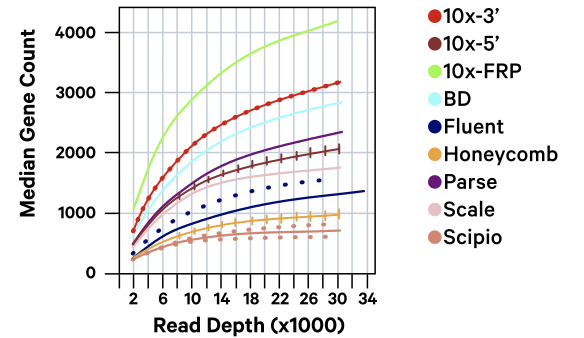
\includegraphics[width=0.9\textwidth]{./figures/sequal.png}
  \caption{The number of genes detected per reads for different single-cell technologies.}
  \label{fig:sequal}
\end{figure}

It might be solved by new technologies, indeed we now have technologies like VASA-seq \cite{salmenHighthroughputTotalRNA2022}, 10X's Flex \cite{llora-batlle10xGenomicsGene2024}, and smart-seq 3 \cite{hagemann-jensenSinglecellRNACounting2020} that promise unparalleled definition for a given sequencing budget. The number of genes they can discover per cell, which is a measure of quality of the sequencing has increased by 50\% compared to 10x v3. 

Another issue is the set of cells that can be assessed and their fidelity to what was initially sent for sequencing. 10x's Xenium, BGI's STEREO-seq, and expansion-based in situ method~ \cite{alonExpansionSequencingSpatially2021} are promising for sequencing RNAs in their original 2D or even 3D context within sub-cellular locations for millions of cells at once. Without manupulating the cells and creating droplets. Solving many issues of current technologies. But we will also have to be smarter in how we select cells to sequence. 

\section{Multi modality \& perturbations}

Indeed, these two modalities and their tradeoffs exist within a range of other techniques often needed to make sense of RNA biology itself.

Interventional data is also required for the model to learn causality, especially when assessed at multiple fine-grained timescales and in higher-quality cellular models such as organoids. Imaging-based methods can also achieve higher throughput, lower prices without destroying the cells.

\begin{figure}[ht]
  \centering
  \includegraphics[width=0.9\textwidth]{./figures/minibrains.png}
  \caption{Image of brain organoids from the Broad Institute}
  \label{fig:organoids}
\end{figure}

But the search space remains unfathomable. it is not just every genes that one would want to perturb, it is the hundreds of millions of locations that might create a specific effect. It is not just in one cell but in the many possible cell states. It is not just one element but multiple at a time, not just one time point but many, not just one readout. Tools like digital microfluidics \cite{yuFieldProgrammableDigital2023} might allow us to solve some of these problems by providing precise control over which cells receive specific perturbations and obtain particular readouts, instead of pooling experiments and sequencing budgets randomly. If paired with AI models and online active learning, we might some day, have a shot at creating a true AI-virtual cell.

\section{The AI virtual cell}

We have seen barely glimpses of the idea of an AI-based virtual cell modeling in this thesis. But it is undeniably through the above-mentioned techniques that more work will be needed. Indeed, the goal of an virtual cell is to be able to predict the state of a cell through time, as it interacts with and gets perturbed by its environment. With the advent of \gls{CRISPR}-screens, and drug-seq, a focus has been put on predicting the effect of a drug on a dissociated cell after a given period of time. this can be on: its survival, its morphology or its expression profile. Many big projects have been launched such as DepMap \cite{DepMapPanCancerBiomarker} and Recursion's RxRx database \cite{fayRxRx3PhenomicsMap2023}. More recently, the Arc Virtual Cell Challenge \cite{bunneHowBuildVirtual2024}, also highlighted how limited our current technology and benchmarks are, with AI models achieving poor performances, the limited usability of cross-lab data and metrics that were easily gamed.

But most data is and will remain generated through the thousands of labs across the world. Most of the time siloed. Training on these public noisy, static and poorly labelled datasets is often called pretraining. While the above-mentionned techniques could be seen as reinforcement learning with active feedback (RLAF). Such an AI-VC model would have been pretrained on most of the available biological data, using foundation models of single-cell multimodalities, tissues, molecules, and protein-RNA-DNA sequences, pooled together in the kind of approaches we described in Chapter 2. LLMs could allow rich reasoning across these representations, results, and the breadth of written human knowledge.

Finally, the hope is to drive experiments in the lab and perform hypothesis generations that could be transfered from cheap in silico experiments to more expensive in vitro experiments on dissociated cells, organoids and finally to in vivo models. This loop of pretraining, RLAF, and hypothesis generation is what we call the lab in the loop approach to cellular modeling (Figure \ref{fig:labinloop}).

\begin{figure}[ht]
  \centering
  \includegraphics[width=0.9\textwidth]{./figures/lab-in-the-loop.jpg}
  \caption{overview of the lab in the loop approach to cellular modeling. from the AIVC perspective paper \cite{bunneHowBuildVirtual2024}.}
  \label{fig:labinloop}
\end{figure}

Many challenges remain in bridging fields such as data engineering, machine learning, material engineering, microelectronics, molecular biology, and cell biology, but the rewards are tremendous, as many diseases won't be solved by brute force approach or by targeting one specific gene, whether cancer or other complex multi-cellular aging diseases.

\newpage\thispagestyle{empty}

\fancyhead{} % clear all header fields
\fancyhead[OL]{\textsc{Conclusion}}
\chapter{Conclusion} % Main chapter title
%\addcontentsline{toc}{chapter}{Conclusion générale}  
%\startcontents[chapters]
%\pagestyle{plain} % remove headers/footers from the chapt\markboth{Left}{Right}

%\pagestyle{fancy}
%\renewcommand{\chaptermark}[1]{\markboth{Chapter \thechapter. #1}{}}
%\renewcommand{\sectionmark}[1]{\markright{\thesection\ #1}}

Single-cell Foundation Models while in their infancy, have the power to change the way we do biology and medicine.

\vspace{13pt}

During this Thesis, we have shown that:

\begin{itemize}[label=\textbullet]%[label=$\ast$]
        \item We can use the internal workings of scFMs to predict meaningful gene interactions.
        \item We can update their training tasks, data, losses, as well as their architectures to better capture the underlying biology of the cell.
        \item We can use them to perform a variety of single cell tasks in a zero-shot of few-shot manner, from cell annotations, denoising, imputation, embeddings generation, batch correction, cross-species integration and counterfactual reasoning
        \item We can use multiple techniques at inference and fine-tuning time to improve their performance.
        \item We can leverage the other foundation models pretrained on other modalities to improve their performance.
\end{itemize}

\vspace{13pt}

In conclusion, the follow-up of these studies should allow to multiply the use-cases of single-cell transcriptomics in clinical applications, creating better benchmarks of models and in turn better models. It would be to integrate other modalities like sequences, epigenetics, proteomics, spatial, and imaging via multi-scale architecture and fine-tuning. But also allow these models to reason by integrating them to LLMs. Finally one will need to gather more data from novel species, patient contexts and across perturbations. To the later point especially we will want to use active learning to guide the experiments and eventually reach the grand goal of cellular modeling.


%----------------------------------------------------------------------------------------
%	BIBLIOGRAPHY
%----------------------------------------------------------------------------------------
%\printbibliography %Prints bibliography
\fancyhead{} % clear all header fields
\fancyhead[OL]{\textsc{Bibliography}}
\printbibliography[
heading=bibintoc,
title={Bibliography}]

%----------------------------------------------------------------------------------------
\fancyhead{} % clear all header fields
\fancyhead[OL]{\textsc{Appendices}}


\includepdf[pages=-]{chapters/supplementary_scprint.pdf}
\label{sec:suppscprint}

% The following file is missing:
% \includepdf[pages=-]{chapters/supplementary_scprint2.pdf}
% \label{sec:suppscprint2}

\end{document}
